% !TeX spellcheck = fr_FR
% Fichier hdr.tex
% Auteur : Luiz Angelo Steffenel
% CReSTIC SysCom, Université de Reims, France
% Date de création : 17 janvier 2014
% Dernière mise à jour : 17 janvier 2014

%+++++++++++++++++++++++++++++++++++++++++++++++++++++++++++++++++++++++++++++
%+++++++++++++++++++++++++++++++++++++++++++++++++++++++++++++++++++++++++++++
%
%+++++++++++++++++++++++++++++++++++++++++++++++++++++++++++++++++++++++++++++
%+++++++++++++++++++++++++++++++++++++++++++++++++++++++++++++++++++++++++++++

\documentclass[final,twoside]{hdr} % final
%\documentclass[preliminary,nodate,oneside]{hdr}
\usepackage{times}
\usepackage[T1]{fontenc}
\usepackage[utf8]{inputenc}
\usepackage[english,frenchb]{babel}
\usepackage{listings}
\usepackage{hyperref}
\usepackage{subfigure}
\lstset{language=c,frame=LBtr,extendedchars=true}
%\usepackage{prog}
\usepackage{url}
%\usepackage{isolatin1}


\usepackage{amsmath}
\usepackage{amsfonts,amssymb}
\usepackage[boxed]{algorithm}
\usepackage{algorithmic}
\usepackage[]{graphics}
\usepackage{rotating}
\usepackage{multirow}

\usepackage{fancybox}
%%%%%%%%%%%%%%%%%%%%%%%%%%%%%%%%%%%%%%%%%%%%%%%%%%%%%%%%%%%%%%%%%%%
% redefinition des commandes du package algorithm & algorithmic

\renewcommand{\algorithmicif}{{\bf SI}}
\renewcommand{\algorithmicthen}{{\bf ALORS}}
\renewcommand{\algorithmicelse}{{\bf SINON}}
\renewcommand{\algorithmicend}{{\bf FIN}}
\renewcommand{\algorithmicwhile}{{\bf TANTQUE}}
\renewcommand{\algorithmicfor}{{\bf POUR}}
\renewcommand{\algorithmicforall}{{\bf POUR TOUT}}
\renewcommand{\algorithmicdo}{{\bf FAIRE}}
\renewcommand{\algorithmicelsif}{{\bf SINON SI}}

\floatname{algorithm}{Algorithme}
\renewcommand{\listalgorithmname}{Liste des algorithmes}

%%%%%%%%%%%%%%%%%%%%%%%%%%%%%%%%%%%%%%%%%%%%%%%%%%%%%%%%%%%%%%%%%%%%%

%\newtheorem{definition}{Définition}
\newenvironment{definition}
  {\vspace{.5em} \noindent {\bf Définition : }}
  {\vspace{.5em}}

\newenvironment{remarque}
  {\vspace{.5em} \noindent {\bf Remarque : }}
  {\vspace{.5em}}

\newenvironment{lemme}
  {\vspace{.5em} \noindent {\bf Lemme : }}
  {\vspace{.5em}}

\newtheorem{corollaire}{Corollaire}
%\newtheorem{lemme}{Lemme}
\newtheorem{theoreme}{Théorème}
\newtheorem{proposition}{Proposition}
\newtheorem{propriete}{Propriété}
%\newtheorem{remarque}{Remarque}
\newcommand{\thethm}{} 

\newenvironment{resume}{%
  \noindent\rule{\linewidth}{.1pt}\par\nobreak\vskip-1em%
  \vspace{1em}\noindent\textbf{Résumé}\par\nobreak\vskip1em%
  \noindent\itshape}%
 {\par\nobreak\noindent\rule{\linewidth}{.1pt}}

%\pagestyle{myheadings}
\renewcommand{\soutname}{Soutenue publiquement le }


%\let\urlorig\url
%\renewcommand{\url}[1]{
%	\begin{otherlanguage}{english}\urlorig{#1}\end{otherlanguage}
%}

\def\imagetop#1{\vtop{\null\hbox{#1}}}

\usepackage{pstricks}
\usepackage{colortab}
\usepackage{verbatim}
\usepackage{verbatimbox}

\begin{document}

\title{Contributions à la Gestion de l'Hétérogénéité dans les Environnements Distribués \\et Pervasifs}
\author{Luiz Angelo STEFFENEL}
\date{8 décembre 2017}

\jury{
     {\em Président du jury} :                
                                        & Carine \fsc{Souveyet} &
                                        Professeur à l'Université Paris 1 Panthéon-Sorbonne\\
{\em Rapporteurs} :          &  Christophe \fsc{Cérin} &
                                        Professeur à l'Université Paris 13 - IUT Villetaneuse\\
                                        &  Emmanuel \fsc{Jeannot} & 
										Directeur de Recherche, INRIA Bordeaux Sud-Ouest\\
                                        & Philippe \fsc{Roose}   &
										Maître de Conférences HDR à l'Université de Bayonne\\
{\em Examinateurs}:         & Massimo \fsc{Villari} &
                                        Professeur à l'Università degli Studi di Messina, Italie\\
                                         & Michaël \fsc{Krajecki}   &
                                        Professeur à l'Université de Reims Champagne-Ardenne\\
	{\em Directeur} :           & Olivier \fsc{Flauzac}        & 
                                        Professeur à l'Université de Reims Champagne-Ardenne\\
                                        }
\maketitle

\begin{dedication}
à Manuele.
\end{dedication}

\begin{thanks}
{Je tiens à exprimer mes remerciements et toute ma gratitude à :}

%\item Franck Cappelo, qui m'a fait l'honneur de bien vouloir présider
%  le jury.
%
%\item P. Felber, H. Guyennet et I. Lavallée, qui ont tous trois accepté de
%  rapporter cette habilitation.
%
%\item Merci à V. Villain qui après m'avoir << initié >> à la recherche
%  il y a quelques années, a accepté de particier à mon jury.
%
%\item Je remercie A. Bui, directeur de l'équipe de recherche LICA. Son
%  soutien sans faille depuis mon arrivée à Reims, ainsi que les
%  conseils avisés qu'il m'a prodigués ont contribué à la préparation de
%  cette habilitation, ainsi qu'au développement de différents projets.
%
%\item Merci à l'ensemble de l'équipe LICA, et plus particulièrement à
%  M. Krajecki et P.-P. Mérel, avec lesquels << l'aventure >> CONFIIT a
%  été initiée et se poursuit, ainsi qu'à H.~Fouchal.
%
\item Je remercie les étudiants qui m'ont fait confiance pour
%  l'encadrement de leurs travaux de doctorat : T.~Bernard et C.~Rabat.
%
%\item Pour finir ces remerciements, je n'oublie pas ma famille, mon
%  épouse Hélène dont le soutien au quotidien à contribué à l'ensemble
%  du travail réalisé, à Michelle dont les premiers pas et les joyeux
%  << gazouillis >> ont rythmé la rédaction de cette habilitation, sans
%  oublier mon père qui a toujours cru en moi et m'a toujours soutenu,
%  et ma mère, pour laquelle j'ai une pensée particulière.
\end{thanks}

\tableofcontents

\Bigchapter{Introduction}

% !TeX spellcheck = fr_FR

La définition du mot \textbf{hétérogénéité} donné par le Dictionnaire Larousse ("\textit{Manque d'unité, composé d'éléments de nature diverse}") n'est pas suffisamment développée pour qualifier les différents défis liés à l'hétérogénéité dans les systèmes et applications distribués. Afin de mieux comprendre ces défis, il est important d'identifier et de cataloguer les différents mécanismes liés à l'hétérogénéité.

Une première catégorie est issue directement de la définition simple ci-dessus, et représente les variations des équipements composant un système informatique. Sous cette optique, l'hétérogénéité se présente comme une conséquence de la différente construction des dispositifs qui composent le système, notamment leur composition matérielle (processeurs, mémoire) et leur capacité de calcul. Ainsi, un système distribué composé d'équipements identiques (caractérisé par l'absence d'hétérogénéité matérielle) peut supposer un traitement uniforme des tâches de calcul et de traitement de données, et donc simplifier la gestion des applications qu'y tournent. Au contraire, un système composé par des équipements hétérogènes, même partiellement, doit être conscient de cette différence et prévoir des mécanismes pour garantir l'exécution des applications : synchronisation des tâches dépendantes, ordonnancement selon les capacités des équipements, équilibrage et migration de charge, etc.  Même étant très réductrice, \textit{l'hétérogénéité matérielle} est souvent utilisée pour qualifier des équipements : machines parallèles (symétriques), clusters (grappes d'ordinateurs), grids (grilles de calcul), cloud, réseaux ad-hoc et P2P, etc.

À l'hétérogénéité matérielle s'ajoute le problème de l'\textit{hétérogénéité des communications}, qui peut être causé autant par la diversité matérielle (par exemple, en utilisant différentes technologies réseau) ou par la distance géographique (qui impacte les temps de communication). On retrouve l'hétérogénéité des communications surtout dans les systèmes distribués à grande échelle (grids, réseaux P2P) où le temps de communication devient un facteur non négligeable. La prise en charge de l'hétérogénéité des communications se fait notamment par l'optimisation des dépendances : limitation des communications sur les grandes distances,  recouvrement des communications par de calculs, ordonnancement basé sur la topologie du réseau, etc. Toutefois, cette prise en charge ne peut pas se faire sans une connaissance des facteurs impactant la communication, d'où la nécessité de mesurer et modéliser les communications. 

Il est claire que la diversité matérielle et la diversité des communications (matérielle ou spatiale) constituent les facteurs les plus importants liés à l'hétérogénéité à un moment donné de l'exécution d'une application, toutefois ce ne sont pas les seuls éléments impactant le déroulement de son exécution. Plus qu'assurer des bonnes conditions à un moment ou opération précis, nous devons garantir le fonctionnement d'un système distribué malgré les variations qu'il subit pendant la durée de son fonctionnement. Cette forme d'hétérogénéité "\textit{temporelle}" est issue de la dynamicité de l'opération d'un système. Plus exactement, les systèmes distribués peuvent être impactés par le départ ou l'arrivé de ressources, mais aussi par leur changement d'état ou de capacité. De ce fait, la prise en compte de ces facteurs devient essentiel pour le bon fonctionnement d'un système et d'une application. La prise en charge de la dynamicité implique plusieurs éléments : la surveillance des ressources et la détection des pannes/états invalides, le suivi et la récupération des tâches attribuées à des éléments disparus et aussi le rééquilibrage de charge dans le cas d'une augmentation des ressources disponibles. En effet, la dynamicité affecte l'utilisation des ressources, car même sans une défaillance un système doit pouvoir être amené à gérer plusieurs tâches indépendantes, chacune avec des besoins propres.

D'un point de vue applicatif, nous pouvons aussi rencontrer des difficultés avec une tout autres catégorie d'hétérogénéité, transversale aux trois précédentes :\textit{ l'hétérogénéité des données}. En effet, le développement d'une application est souvent guidé par la manière dont on accède aux données, et le \textit{big data} a mis en évidence le besoin de gérer non seulement des grandes volumes de données mais surtout leur variété. Les données peuvent se présenter sous des abstractions bien connues comme par exemple les objets dans la mémoire, les fichiers, les URIs ou les requêtes distantes (RPC, web services, etc.). Toutefois, il est rare qu'une application dispose d'un accès uniforme à tout type de donnée, ce qui implicitement introduit de l'hétérogénéité au niveau de l'accès aux données et à leur traitement. 

Mon travail de recherche s'inscrit donc dans la gestion de l'hétérogénéité, sous ses différentes facettes. En navigant entre ces aspects, j'ai pu travailler à la fois sur la tolérance aux fautes, la modélisation des performances, l'adaptation au contexte et l'ordonnancement, et même la spécification et développement d'intergiciels (\textit{middlewares}) pour le calcul distribué. Bien souvent j'ai pu profiter des collaborations et projets dont j'ai été membre ou responsable pour introduire ou explorer des éléments liés à la gestion de l'hétérogénéité, tout comme dans les thèses de doctorat que j'ai co-encadré. 

Ce mémoire présente une partie de ces contributions, toutes ayant fait l'objet de publications dans des journaux et conférences internationaux, mais aussi d'autres communications qui se trouvent sur la liste récapitulative à la fin de cet ouvrage. Le mémoire est organisé en cinq parties, dans lesquelles j'expose les différents aspects de mes travaux de recherche visant la gestion de d'hétérogénéité :
\begin{description}
	\item[i] l'évaluation et la modélisation des performances de communication dans les grids; 
	\item [ii] la parallélisation et la gestion de l'hétérogénéité des tâches ;
	\item [iii] l'adaptation à la dynamicité des ressources de calcul ;
	\item [iv] la spécification d'une plate-forme pair-à-pair visant l'accès à différentes sources de données ;
	\item [v] la conception et le développement d'un intergiciel pair-à-pair pour le calcul distribué dans des environnements hétérogènes tels que le \textit{fog computing} et l'Internet des Objets.
\end{description}


Dans la première partie, je présente des algorithmes originaux issus des travaux menés à la fin de ma thèse et dans les trois années subséquentes. Ces travaux visaient notamment la compréhension des facteurs impactant les opérations de communication collective dans les grids de calcul, et dont le but ultime était à la fois d'optimiser ces opérations mais aussi de pouvoir estimer leur performance avec haute précision.  J'exploite ainsi des méthodes de mesure de performance et de découverte de la topologie réseau afin de représenter correctement les environnements et pouvoir extraire des indicateurs aidant à choisir les algorithmes de communication collective les plus adaptés à chaque situation. 

Dans la deuxième partie j'illustre les efforts pour la parallélisation et la gestion de l'exécution distribuée d'une application métier en biochimie. Ce travail a été développé dans le cadre du co-encadrement de thèse de doctorat de Romain Vasseur (thèse CIFRE en collaboration avec le Laboratoire MeDyC - Matrice Extracellulaire et Dynamique Cellulaire - UMR CNRS 7369 et la compagnie Bull-Atos), et visait le développement de stratégies HPC pour le \textit{docking inversé}, une technique de simulation des interactions biomoléculaires. Comme il n'était pas envisageable de paralléliser le code source de l'application, nous avons opté par le développement de stratégies visant à découper convenablement l'espace de recherche et permettre le traitement parallèle des tâches de calcul. Ceci a été accompagné par le développement d'une plate-forme de déploiement capable de gérer l'exécution des tâches distribuées sur plusieurs n{\oe}uds ou bien de tirer profit des gestionnaires de tâches présents sur la plupart des clusters HPC. 

La troisième partie de ce mémoire s'attaque à la dynamicité des ressources et aux stratégies pour s'adapter à ces changements. Plus exactement, on reprend une partie des travaux effectués pendant le projet STIC-AmSud PER-MARE dans lequel nous avons apporté des améliorations à la plate-forme \textit{big data} Apache Hadoop afin de la rendre compatible avec des environnements hétérogènes et dynamiques (environnements pervasifs). Grâce à un mécanisme de collecte d'informations sur le contexte des ressources de calcul, nous avons modifié l'ordonnanceur de Hadoop afin d'adapter le lancement de tâches aux ressources disponibles à chaque instant. Outre la présentation du mécanisme de collecte de contexte et des stratégies d'intégration à Hadoop, cette partie inclut des \textit{benchmarks} démontrant l'efficacité des solutions proposées. 

La quatrième partie présente la spécification d'une plate-forme distribuée pour la gestion universelle de données, résultat do co-encadrement de la thèse de doctorat de Thierno Ahmadou Diallo (thèse en co-tutelle avec l'Université Cheikh Anta Diop, Sénégal). La motivation pour ce travail a été celle de créer une base documentaire indépendante de la nature des données (fichiers, flux, bases de données, etc.) et qui pourrait être utilisée par les universités et écoles de l'Afrique, dans lesquelles l'accès au cloud n'est pas toujours évident à cause des vitesses d'interconnexion. Dans ce travail je présente seulement la partie dédiée à la spécification de la plate-forme GRAPP\&S, le cas d'usage retenu pendant la thèse (utilisation de la plate-forme pour pour le \textit{e-learning}) n'étant pas d'intérêt direct pour ce mémoire. 

Finalement, la cinquième partie introduit la plate-forme de calcul distribué CloudFIT. Développée initialement dans le cadre du projet STIC-AmSud PER-MARE, CloudFIT s'est révélé une excellente plate-forme expérimentale pour le prototypage et le test de techniques pour le \textit{fog computing} et l'Internet des Objets. Dans un premier moment nous présentons l'architecture et les mécanismes de communication et de gestion des n{oe}uds. Par la suite, on introduit des stratégies pour l'ordonnancement adapté au contexte nécessaires au support à des ressources de calcul très hétérogènes, allant des dispositifs IoT aux datacenters et cloud. Cette variété de ressources et un élément clé du \textit{fog computing}, que nous embrassons en proposant des stratégies pour la structuration multi-échelle du réseau ou bien de techniques pour renforcer la \textit{data-locality}. Cette partie se termine par la présentation de deux travaux où CloudFIT a été utilisé en tant que plate-forme de calcul. Dans le premier cas, il s'agit de l'exécution d'une application \textit{big data} bien connue. Dans le deuxième cas, nous présentons la spécification et l'implémentation d'une application en physique de l'atmosphère destinée à la surveillance d'événements liés à la couche d'Ozone Antarctique. 

Je conclurai enfin ce document en présentant les perspectives de recherche que j'espère pouvoir développer dans un avenir proche.


 



\chapter{L'Hétérogénéité des Communications}

\begin{resume}
Dans l'ensemble des éléments qui composent les systèmes informatiques, les réseaux informatiques sont parmi les éléments qui sont les plus exposés et impactés par l'hétérogénéité. Cette hétérogénéité peut se présenter sous différéntes formes : diversité d'équipements et de technologies, variations de performance et disponibilité (volatilité), limitations liées aux caractéristiques physiques ou à la capacité des ressources, etc. 

Si cette hétérogénéité doit être prise en compte lors du développement de systèmes et applications, il s'avère souvent que les solutions se limitent à pallier les éventuels problèmes. Les travaux que j'ai mené dans le domaine de l'hétérogénéité des réseaux visent la compréhension des facteurs liés à l'hétérogénéité, leur caractérisation et aussi l'optimisation de l'usage des ressources afin de rendre les systèmes et applications plus performants et fiables.

L'une des premières étapes dans l'étude de l'hétérogénéité requiert l'observation et l'analyse des communications réseau afin de modéliser leur fonctionnement et ainsi permettre une estimation de leurs performances. Cette étude cache néanmoins une grande complexité car même sur un petit ensemble de ressources la variation de certains facteurs peut créer un nombre important de situations, chacune avec un modèle de communication différent. Afin de permettre l'application pratique de cette modélisation de performance nous devons non seulement être en mesure de découvrir la topologie du réseau, mais aussi de pouvoir quantifier les différents facteurs et émettre des hypothèses sur les modèles de communication observés. 

Un mécanisme très utile dans la réduction de la complexité de la modélisation des communications réside dans la classification et catégorisation des ressources observées. Non seulement cela permet de se concentrer sur des modèles "type" qui représentent convenablement des ensembles de ressources, comme aussi on ouvre la possibilité d'utiliser ces informations dans le but d'optimiser les échanges entre les applications.

Dans certains cas, cependant, juste la connaissance des profils de performance peut s'avérer insuffisante, notamment lorsque les applications ont des besoins de fiabilité accrus. Ainsi, l'hétérogénéité dans les réseaux doit aussi s'intéresser à l'observation des ressources afin de détecter des éventuelles défaillances, et de les signaler aux applications et systèmes, qui pourront ainsi réagir et prendre des mesures nécessaires pour assurer ses engagements de fiabilité. 

Dans cette première partie, la Section \ref{sec:reseaux-model} présente les travaux qui ont été menés sur la modélisation et l'évaluation des performances de communication des réseaux. La Section \ref{sec:reseaux-topo} présente les travaux sur la découverte de la topologie et la subséquente classification des ressources. Finalement, la Section \ref{sec:reseaux-defaillances} présente les travaux sur la détection de défaillances. Tous ces éléments sont connectés aux travaux qui seront présentés dans les chapitres suivants.  
%Cette première partie regroupe les travaux que j'ai menés sur la
%structuration des systèmes distribués à l'aide de marches
%aléatoires. Ils constituent la continuité de ceux menés durant ma
%thèse.
%
%J'exploite les marches aléatoires selon deux axes. Le premier consiste
%à n'utiliser que la circulation, sans collecte d'informations au cours
%du déplacement. Le second consiste à combiner les concepts de marche
%aléatoire et de mot circulant, afin d'exploiter l'historique des
%déplacements du jeton.
%
%La première approche m'a permis de définir un algorithme rapide de
%construction et de maintenance d'un arbre couvrant sur un système
%distribué. Cette construction est auto-stabili\-sante, et garantit
%donc la tolérance aux fautes transitoires qui peuvent affecter le
%système.
%
%Dans la seconde approche, l'historique des déplacements est conservé
%dans le jeton, mais n'a aucun impact sur la circulation qui reste
%aléatoire sans mémoire. Le contenu du jeton est analysé et exploité,
%afin de permettre la construction d'arbres couvrants sur chaque
%site. Je propose différents algorithmes auto-stabilisants de gestion
%et de correction du contenu du jeton et de sa circulation. Je dérive
%de cette circulation un algorithme auto-stabilisant garantissant la
%$k-$exclusion mutuelle.
%
%La majorité des travaux présentés dans cette partie, ont été réalisés
%en collaboration avec Alain Bui, professeur à l'université de Reims
%Champagne-Ardenne, et Thibault Bernard, dont je co-encadre une partie
%des travaux de thèse avec Alain Bui.

\end{resume}

\section{Modélisation des Performances d'un Réseau\label{sec:reseaux-model}}

%Dans le contexte de la modélisation de performance, nous appelons
%modèle la description formelle de l'exécution d'un programme sur une
%ou plusieurs machines, de manière à ce que cette description peut
%être utilisée pour comprendre, voire décrire, la performance de tel
%programme.

Une des meilleures manières de comprendre le fonctionnement des algorithmes
distribués et d'évaluer leur efficacité est de modéliser la performance
de ces algorithmes. Si d'un côté il existent certains facteurs non
déterministes qui influencent la performance des applications,
comme par exemple la congestion des ressources, pour la plupart du
temps leur impact sur le temps d'exécution est suffisamment
limité \cite{Grove03}. Ainsi, la plus grande difficulté pour la modélisation
des performances est la correcte représentation des facteurs liés
à la communication entre les processus répartis. Pour cette raison,
la plupart des modèles de performance préfèrent décrire les systèmes
de la manière la plus simple possible ; la perte de précision est
compensée par la simplicité et par la portabilité des solutions à
travers diverses situations et environnements. 

Si les principes de la modélisation de performance peuvent être trouvés
dans des travaux pionniers des années 60 et 70 \cite{Peterson81},
la modélisation de performance a connu une importante attention à
partir des années 80, où des efforts importants ont été faits pour
identifier des modèles de performance adaptés aux technologies et
paradigmes qui ont surgi depuis la décennie précédente. Pour cette
raison, dans ce chapitre nous voulons identifier les modèles qui ont les caractéristiques
les plus adaptées à la modélisation réaliste des communications.


\subsection{Exécution dans les systèmes distribués}

Un système distribué est classiquement défini comme un ensemble
d'unités de traitement ou de calcul indépendantes, reliées entre elles
par des liens de communications. Ces unités de traitement contribuent
au calcul d'un résultat en effectuant leurs exécutions de façon
concurrente.

Un réseau d'interconnexion {\cal R}, aussi appelé système distribué,
est représenté par un graphe $G =(V,E)$, dans lequel $V$ est
l'ensemble des n{\oe}uds et $E$ l'ensemble des arêtes. Les n{\oe}uds
du graphe représentent les sites du réseau, les arêtes du graphe les
liens, ou canaux de communication du réseau.

Par la suite, on parlera indifféremment de n{\oe}ud, de site, de
processus ou de processeur pour définir un n{\oe}ud du réseau. De
même, on parlera indifféremment de canaux ou de liens de communication
pour définir les supports de la communication qu'utilise le réseau.

L'écriture d'un algorithme, ainsi que l'évaluation de ses
performances, ne peut se faire que si l'on a, au préalable, défini un
modèle d'exécution. La modélisation sert à imposer les contraintes
permettant de se rapprocher de la réalité. Les algorithmes distribués
sont écrits selon trois modèles principaux : le modèle à états, le
modèle à registres et le modèle à passage de messages.

Le modèle à états a été défini par Dijkstra \cite{Dij74}. Les sites ne
communiquent pas par l'intermédiaire d'échanges de messages, mais par
leur capacité à lire l'état de la mémoire de leurs voisins. Un site
accède en lecture et en écriture à l'ensemble de son environnement et
aux variables qu'il détient, mais il accède uniquement en lecture à
l'environnement de ses voisins.

Le modèle à registres partagés représente les liens de communication
comme des registres attachés à chaque site. Un lien $l_{ij}$ reliant
les sites $i$ et $j$ "porte" donc un registre $R_{ij}$ dans lequel
le site $i$ écrit les informations à transmettre au site $j$. De même,
il existe un registre $R_{ji}$ utilisé par le site $j$ pour
transmettre des informations au site $j$.

Le modèle à passage de messages définit des canaux de communication
par lesquels transitent les messages. Il nécessite de poser des
hypothèses sur les propriétés des canaux de communication : taille,
délais de transmission, caractéristiques des échanges...

Les différents modèles permettent une approche progressive des
communications dans les systèmes distribués. Lynch \cite{Lyn96}
propose toutefois des algorithmes et des méthodes permettant de
transformer un algorithme écrit pour un modèle à registres partagés en
un algorithme exploitant le modèle à passage de messages.

Dans notre cas spécifique, nous voulons explorer le modèle à passage de messages,
étudiant notamment les modèles de performance qui peuvent apporter à la fois une
représentation fidèle du comportement des communications mais aussi une 
utilisation simple, capable d'être appliquée sur des environnements hétérogènes.

%\subsection{Hockney}
%
%Le modèle de Hockney \cite{Hockney94} est un des plus utilisés pour
%décrire la communication point-à-point dans les machines parallèles
%à mémoire distribuée. Selon ce modèle, une communication entre deux
%noeuds est décrite par : 
%
%\[
%t=t_{0}+\frac{m}{r_{\infty}}\]
%
%
%où $t_{0}$ représente le temps nécessaire à l'envoi d'un message
%de taille zéro, \emph{m} est la taille du message (en octets) et $r_{\infty}$
%est le débit asymptotique en Moctets/s, i.e., le débit maximal obtenu
%quand la taille du message s'approche de l'infini. Dans ce raisonnement,
%$m/r_{\infty}$ représente le délai de transmission d'un message de
%\emph{m} octets à travers un réseau avec un débit asymptotique de
%$r_{\infty}$ Moctets/s.
%
%Ce modèle est souvent transformé dans l'équation affine 
%
%\[
%t=\alpha+\beta m\]
%
%
%où $\alpha$ correspond à la latence de transmission et $\beta$ est
%le temps de transfert d'un octet sur ce réseau \cite{Pjesivac-Grbovic05}.
%L'obtention des paramètres $\alpha$ et $\beta$ peut se faire à travers
%l'utilisation de certains outils comme NWS \cite{Wolski97}. 
%
%Toutefois, un inconvénient de ce modèle est qu'il assume que le temps
%de transfert est proportionnel à la taille du message. Dans des situations
%réelles, certains facteurs comme la taille de la mémoire tampon et
%la segmentation des messages en paquets font varier le temps de transfert
%$\beta$ selon la taille du message. 
%
%\subsection{Postal}
%
%À partir de l'observation qu'un des principaux paramètres pour la
%modélisation des algorithmes parallèles est le coût de communication
%entre les processus, Bar-Noy et Kipnis ont proposé le modèle Postal
%\cite{Bar-Noy94}. Le modèle Postal est fondé sur un paramètre $\lambda=t_{u}/t_{snd}$,
%où $t_{snd}$ est le temps nécessaire à un processus pour envoyer
%un message (la latence d'envoi), alors que $t_{u}$ représente le
%temps total nécessaire à la réception du message par le processus
%destinataire. Une des innovations du modèle Postal par rapport à ses
%prédécesseurs est que ce modèle permet des situations où un processus
%peut émettre plusieurs messages avant que le premier récepteur a reçu
%son message : cela est dû à une analogie avec l'envoi de lettres par
%la poste. 
%
%Prenons par exemple le cas d'une diffusion ou \emph{broadcast}. Par
%simplicité, il est considéré que $\lambda$ est une valeur entière
%et que le temps est mesuré en cycles, dont la durée est équivalente
%à la latence d'envoi d'un message. Dans le cas du \emph{Broadcast},
%la valeur de $\lambda$ influence la forme de l'arbre de diffusion
%qui permet la meilleure performance. C'est ainsi que la Figure \ref{Figure:Postal Model}
%compare deux arbres de diffusion différents, chacun contenant huit
%noeuds et $\lambda=2$. On observe que l'arbre binomial, (Figure \ref{Figure:Postal Model}a),
%malgré son optimalité quand $\lambda=1$, nécessite six étapes de
%communication pour compléter l'opération, alors que l'arbre représenté
%dans la Figure \ref{Figure:Postal Model}b nécessite seulement cinq
%étapes. En effet, la construction de l'arbre de diffusion pour \emph{P}
%processus avec le modèle Postal (un arbre-$\lambda$) est fondée sur
%la fonction de Fibonacci généralisée :
%
%\[
%N_{\lambda}(t)=\left\{ \begin{array}{c}
%\begin{array}{cc}
%N_{\lambda}(t-1)+N_{\lambda}(t-\lambda) & \:\:\:\:\:\:\:\:\:\:\:\:\:\:\:\:\:\:\:\:\: si\: t\geq\lambda,\\
%1 & dans\: le\: cas\: contraire\end{array}\end{array}\right.\]
%
%
%Dans ce cas, $N_{\lambda}(t)$ représente le nombre maximum de noeuds
%qui peuvent être contactés à l'instant \emph{t} sur une architecture
%réseau \emph{1-port}. Si $t<\lambda$, seul le noeud source peut détenir
%le message à l'instant \emph{t}. Par contre, si $t\geq\lambda$, le
%nombre de noeuds contactés est la somme de deux éléments. Le premier
%élément, $N_{\lambda}(t-1)$, indique le nombre de noeuds qui ont
%été contactés jusqu'à l'instant précédent. Le deuxième facteur, $N_{\lambda}(t-\lambda)$,
%indique le nombre maximum de noeuds qui peuvent être contactés à l'instant
%\emph{t}. 
%
%%
%\begin{figure}[h]
%\begin{centering}
%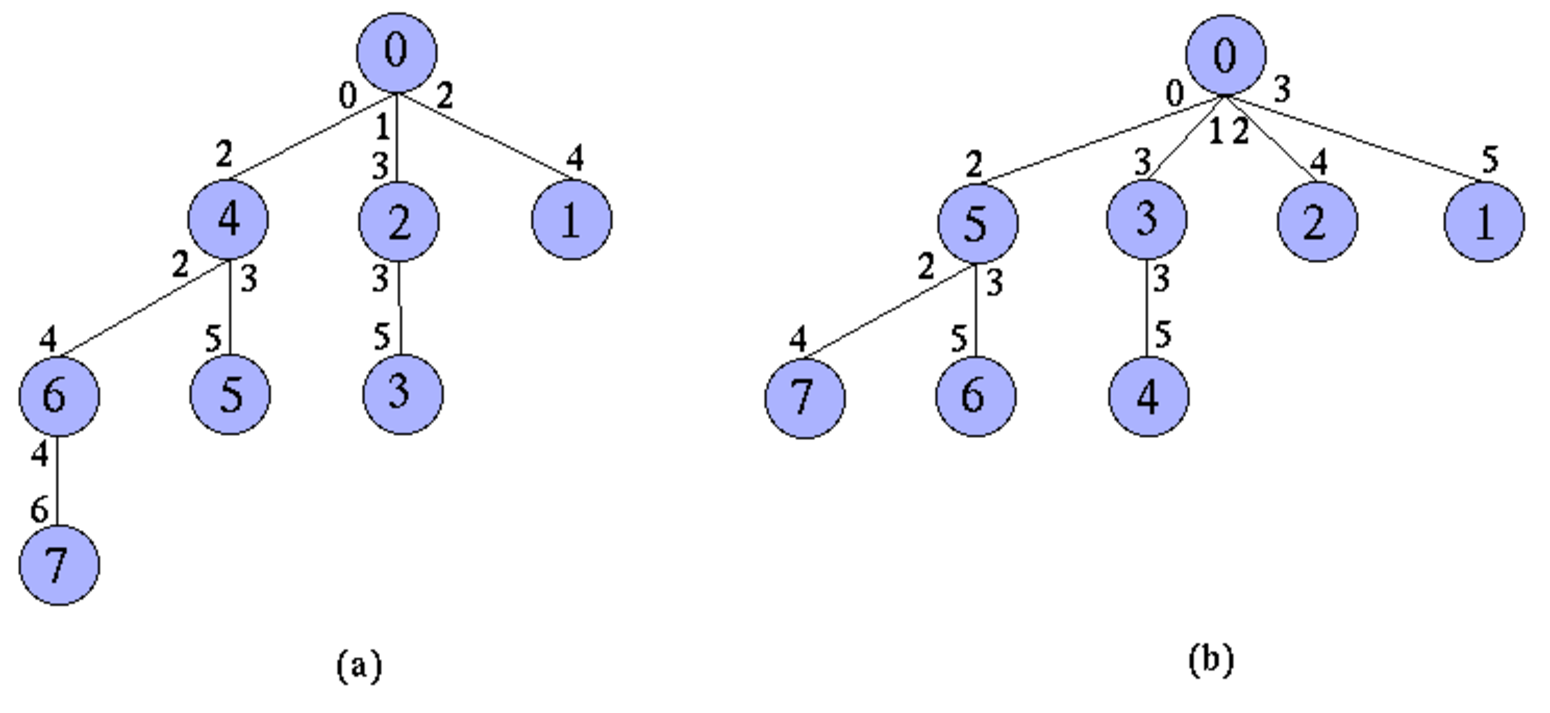
\includegraphics[width=0.85\linewidth]{images/p2p/postal-bcast}
%\par\end{centering}
%
%\caption{\label{Figure:Postal Model}Broadcast avec $\lambda=2$:arbre binomial
%et arbre-$\lambda$}
%
%\end{figure}
%


\subsection{Modélisation des Communications}

Malgré le développement de processeurs et de réseaux plus efficaces,
la communication efficace entre ces deux éléments a toujours été un
obstacle à l'obtention de meilleures performances. En effet, l'augmentation
du nombre de processeurs ne permet pas nécessairement que le temps
d'une application soit réduit proportionnellement : en dehors des
limitations dues au grain des tâches, le coût de communication entre
les différents processeurs est l'un des plus importants obstacles.

Le modèle de Hockney \cite{Hockney94} est un des plus utilisés pour
décrire la communication point-à-point dans les machines parallèles
à mémoire distribuée. Selon ce modèle, une communication entre deux
noeuds est décrite par : 

\[
t=t_{0}+\frac{m}{r_{\infty}}\]


où $t_{0}$ représente le temps nécessaire à l'envoi d'un message
de taille zéro, \emph{m} est la taille du message (en octets) et $r_{\infty}$
est le débit asymptotique en Moctets/s, i.e., le débit maximal obtenu
quand la taille du message s'approche de l'infini. Dans ce raisonnement,
$m/r_{\infty}$ représente le délai de transmission d'un message de
\emph{m} octets à travers un réseau avec un débit asymptotique de
$r_{\infty}$ Moctets/s.

Ce modèle est souvent transformé dans l'équation affine 

\[
t=\alpha+\beta m\]


où $\alpha$ correspond à la latence de transmission et $\beta$ est
le temps de transfert d'un octet sur ce réseau \cite{Pjesivac-Grbovic05}.
L'obtention des paramètres $\alpha$ et $\beta$ peut se faire à travers
l'utilisation de certains outils comme NWS \cite{Wolski97}. 

Toutefois, un inconvénient de ce modèle est qu'il assume que le temps
de transfert est proportionnel à la taille du message. Dans des situations
réelles, certains facteurs comme la taille de la mémoire tampon et
la segmentation des messages en paquets font varier le temps de transfert
$\beta$ selon la taille du message. 

À partir de l'observation qu'un des principaux paramètres pour la
modélisation des algorithmes parallèles est le coût de communication
entre les processus, Bar-Noy et Kipnis ont proposé le modèle Postal
\cite{Bar-Noy94}. Le modèle Postal est fondé sur un paramètre $\lambda=t_{u}/t_{snd}$,
où $t_{snd}$ est le temps nécessaire à un processus pour envoyer
un message (la latence d'envoi), alors que $t_{u}$ représente le
temps total nécessaire à la réception du message par le processus
destinataire. Une des innovations du modèle Postal par rapport à ses
prédécesseurs est que ce modèle permet des situations où un processus
peut émettre plusieurs messages avant que le premier récepteur a reçu
son message : cela est dû à une analogie avec l'envoi de lettres par
la poste. 

%Ces deux modèles pêchent toutefois par le fait qu'ils considèrent un coût de transmission linéaire par rapport aux tailles des messages, ce qui n'est pas exact. 
%
Dans une tentative de spécifier un modèle de calcul plus réaliste,
Culler \emph{et al.} \cite{Culler96} ont proposé le modèle de coût
LogP afin de permettre la spécification du surcoût d'envoi, qui
est normalement très significatif pour la performance d'un système.
L'importance de ce paramètre est notamment observée sur des expériences
en machines réelles et, surtout, dans le cas des grappes d'ordinateurs. 

%Une autre caractéristique du modèle LogP est son comportement asynchrone. En effet, le modèle LogP ne
%requiert ni barrière de synchronisation, ni super-pas. Quand un processus
%finit l'exécution d'un groupe de tâches et de communications, il peut
%automatiquement avancer vers le prochain groupe de tâches, même s'ils
%existent encore des processeurs travaillant sur une tâche précédente.
%En contraste, le modèle BSP forçait le processeur à rester à l'attente
%de la barrière de synchronisation. Ainsi, ce comportement asynchrone
%du modèle LogP peut être considéré comme un avantage, notamment si
%l'application permet l'avancement asynchrone des différentes lignes
%d'exécution. 

Bien sûr, LogP reste un modèle simplifié des architectures parallèles,
dont certains aspects de la topologie du réseau, comme par exemple
la congestion, ne sont pas directement considérés. Les paramètres LogP qui caractérisent
la communication entre les processus sont les suivants : 

\begin{description}
\item [{L}] - représente la latence de communication entre deux processus
distincts,
\item [{o}] - le surcoût d'initialisation associée à l'envoi/réception
d'un message,
\item [{g}] - aussi appellé "\textit{gap}", cette valeur correspond au temps minimal nécessaire entre deux événements consécutifs
d'envoi ou de réception,
\item [{P}] - le nombre de processus.
\end{description}
Sous cette représentation, le modèle Postal de Bar-Noy et Kipnis devient
un cas spécial du modèle LogP (avec $g=1$ et $o=0$). 

Dans le cas du modèle LogP, le nombre maximum de messages en transit
entre deux processus est de $\lceil L/g\rceil$. La latence maximale
d'un réseau est la distance moyenne asymptotique entre les processus
; toutefois, dans le cas des réseaux fortement hétérogènes, la définition
de ces limites est bien plus complexe. 

%Pour mieux illustrer l'utilisation des paramètres définis par LogP,
%nous présentons dans la Figure \ref{Figure: logp_culler} l'exemple
%proposé par Culler où LogP est utilisé pour décrire le broadcast optimal
%sur un réseau avec $P=8$, $L=6$, $g=4$ et $o=2$. Dans cet exemple,
%nous observons qu'une communication isolée nécessite $o+L+o$ unités
%de temps pour être reçue; cependant, la transmission consécutive de
%deux messages implique un surcoût équivalent à $(g-o)$, car on n'est
%pas autorisé à transmettre deux messages consécutives en moins de
%$g$ unités de temps. En effet, le temps $o$ correspond au temps
%nécessaire au traitement du message pour la transmission (encapsulation,
%mise en mémoire tampon, etc.), alors que le gap $g$ correspond à
%l'intervalle où le réseau reste occupé par la transmission du message.
%
%%
%\begin{figure}[h]
%\begin{centering}
%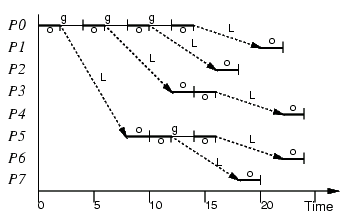
\includegraphics[width=0.6\linewidth]{images/p2p/LogP-optimal}
%\par\end{centering}
%
%\caption{\label{Figure: logp_culler}Diffusion en LogP avec P=8, L=6, g=4 et
%0=2 \cite{Culler96}}
%
%\end{figure}
%


%\subsection{LogGP}
%
%Comme le comportement asynchrone de plusieurs machines parallèles
%et le surcoût de communication sont représentés par le modèle LogP,
%ce modèle est bien plus complet que les modèles précédents. Cependant,
%la faiblesse de ce modèle est que ses paramètres sont établis de façon
%absolue : les valeurs de \emph{g} et \emph{o} sont les mêmes pour
%n'importe quelle taille de message envoyé. Des expériences pratiques
%démontrent que l'utilisation de LogP n'est précise que pour des messages
%de petite taille, dont \emph{g} et \emph{o} ne varient pas trop.
%
%Pour permettre l'utilisation du modèle LogP avec des messages plus
%grands, Alexandrov \emph{et al.} \cite{Alexandrov95} ont présenté
%LogGP, une extension du modèle LogP qui établit le paramètre \emph{G},
%qui représente une valeur de \emph{gap} par octet transmis. À travers
%ce nouveau paramètre, LogGP permet la prédiction du temps de transmission
%d'un message de taille \emph{m} entre deux noeuds avec l'expression
%:
%
%\[
%L+2\times o+(m-1)\times G\]
%
%

\subsection{pLogP}

Le modèle pLogP (\emph{parameterised LogP}) est une extension
du modèle LogP présenté par Kielmann \emph{et al.} \cite{Kielmann01}. Son objectif est de 
mieux représenter à la fois des petits et des grands messages sous un modèle unifié. 

Comme ses prédécesseurs, le modèle pLogP est défini à travers des
paramètres qui représentent la latence, les surcoûts d'initialisation,
le \emph{gap} et le nombre de processus. La première différence est
l'utilisation de valeurs distinctes, $o_{r}$ et $o_{s}$, pour représenter
le surcoût d'envoi et le surcoût de réception d'un message. Toutefois,
la principale caractéristique du modèle pLogP est que les paramètres
qui représentent le \emph{gap} et les surcoûts sont paramétrés selon
la taille du message envoyé. Cela est spécialement important pour
modéliser les communications avec des tailles de messages variables,
une fois que, comme déjà observé par Alexandrov \cite{Alexandrov95},
la performance des communications n'est pas linéaire par rapport à
la taille des messages.

D'autres aspects sont aussi différents, par rapport aux modèles précédents.
En effet, les notions de la latence et du \emph{gap} sont légèrement
différentes de celles utilisées par le modèle LogP. Dans le
cas du modèle pLogP, la latence inclut tous les facteurs qui peuvent
retarder la communication entre deux processus, comme par exemple
la copie de données en mémoire tampon vers les interfaces réseaux,
qui s'ajoutent au temps de transfert des messages déjà considéré par
LogP. Ainsi, dans le cas d'un réseau local, le paramètre \emph{gap}
est défini comme l'intervalle minimale entre deux transmissions ou
réceptions consécutives, ce qui implique que $g(m)\geq os(m)$ et
$g(m)\geq or(m)$ tient toujours. La relation entre ces différents
paramètres est illustrée dans la Figure \ref{Figure: pLogP}. 

%
\begin{figure}[h]
\centering
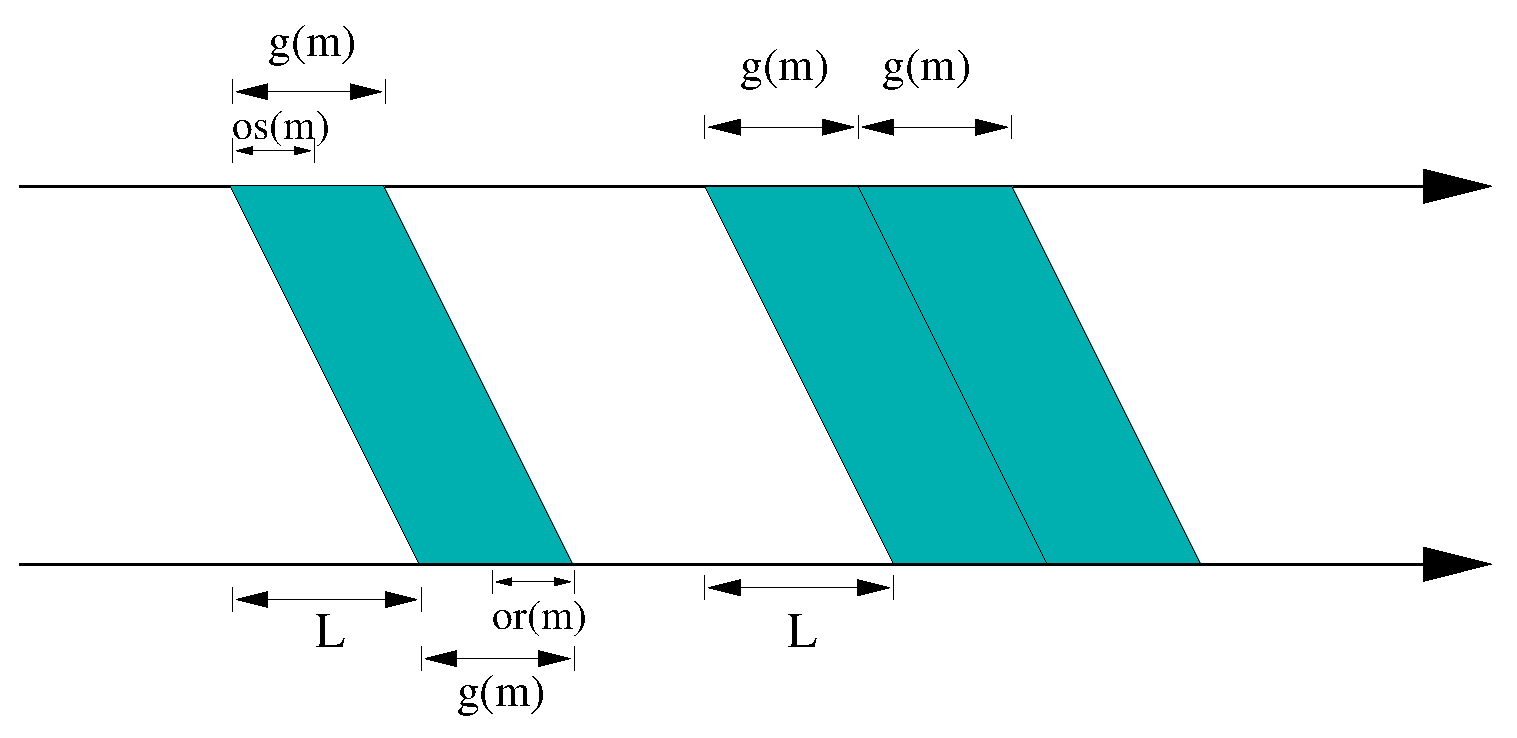
\includegraphics[width=0.7\linewidth]{images/p2p/plogp-struct}

\caption{\label{Figure: pLogP}Représentation d'une communication avec pLogP}

\end{figure}


En conséquence de cette nouvelle interprétation du \emph{gap}, les
paramètres $o_{s}$ et $o_{r}$ ont une importance moins évidente,
une fois que leur coût dans un réseau local est souvent recouvert
par celui du gap.  Ainsi, pour représenter le temps nécessaire à la transmission d'un
message de taille \emph{m} entre deux noeuds avec des primitives de
communication bloquante, le modèle pLogP utilise l'expression $L+g(m)$,
au lieu de $L+g+2o$ comme dans le modèle LogP. 


La variation des paramètres vis-à-vis de la taille des messages et des politiques d'émission est mise en évidence en Figure \ref{Figure: logp x hockney}, où on affiche les différents temps de communication mesurés avec la bibliothèque applicative LAM-MPI \cite{LAM04}. On observe un
changement de politique d'acquittement quand la taille des messages dépasse les 64 Ko, de manière à ce que le coût du gap dépend à la fois
de la saturation de la fenêtre TCP et de la politique d'acquittement.

%
\begin{figure}
\centering
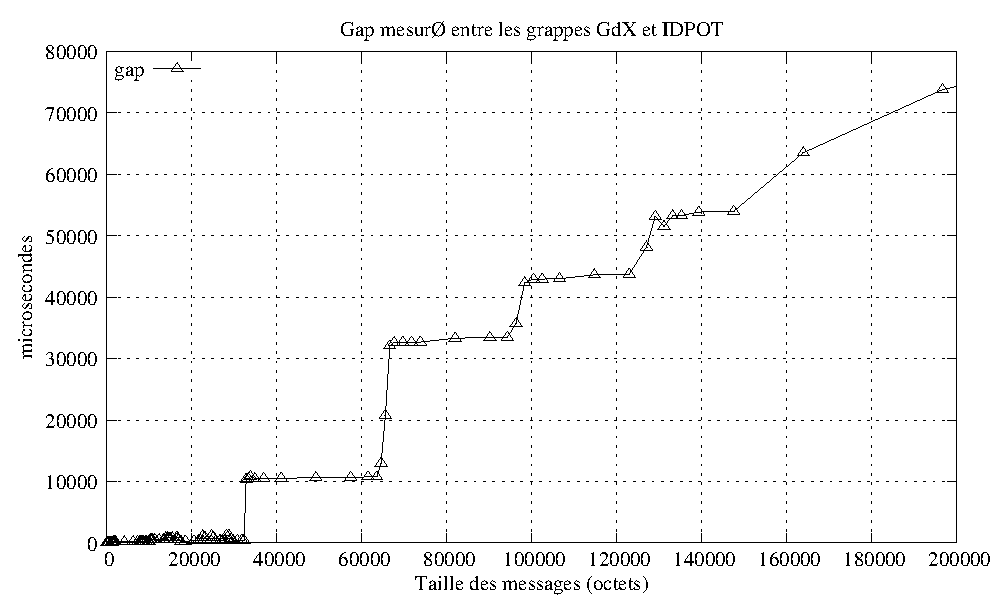
\includegraphics[width=0.7\linewidth]{images/p2p/hockney-logp1}

\caption{\label{Figure: logp x hockney}Valeurs de gap mesurés entre deux grappes
distantes (GdX et IDPOT)}

\end{figure}

\subsection{\label{sec:Broadcast}Exemple d'utilisation: modélisation d'un Broadcast\emph{: MPI\_Bcast}}

Une opération de \emph{Broadcast} s'effectue quand un seul processus,
appelé \emph{racine,} envoie le même message de taille \emph{m} à
tous les autres $(P-1)$ processus. 


L'approche classique pour implémenter l'opération \emph{Broadcast} utilise
des arbres qui sont décrits par deux paramètres, \emph{d} et \emph{h},
où \emph{d} est le nombre maximum de successeurs qu'un noeud peut
avoir, et \emph{h} est la hauteur de cet arbre, le chemin le plus
long qui relie la racine et les feuilles de cet arbre. Plus généralement,
des arbres de diffusion avec différents degrés \emph{d} et \emph{h}
peuvent être générés à partir d'un algorithme de type \emph{arbre-alpha}
(\emph{alpha-tree} en anglais) suggéré par Bernaschi et Ianello \cite{Bernaschi98}.
À l'aide de cet algorithme et des paramètres du réseau, un arbre optimal
peut être construit à partir des paramètres du réseau et avec \emph{d,
	h $\in$}{[}1...\emph{P}-1] tel que $\sum_{i=o}^{h}d^{i}\geq P$ soit
respecté. %Cependant, pour une question de simplicité, la plupart des
%implémentations MPI utilisent des formes fixes telles que les arbres
%plats ou les arbres binomiaux. 

La performance des différentes formes fixes dépend surtout des paramètres
du réseau, notamment le \emph{gap}, la latence et le nombre de noeuds.
Par conséquent, un réseau avec une latence faible par rapport au \emph{gap}
favorise les algorithmes de type Arbre Binaire et Arbre Binomial,
qui cherchent à minimiser le temps de communication par la multiplication
des sources de transmission. Au contraire, si la latence est trop
élevée par rapport au \emph{gap}, les algorithmes de type Arbre Plat
sont favorisés, où un seul processus envoie des messages à tous les
autres. 

%De ce fait, la plupart des implémentations MPI utilisent deux formes
%fixes, un Arbre Plat pour un nombre réduit de noeuds (jusqu'à 3 noeuds),
%et un Arbre Binomial pour un plus grand nombre de noeuds. Cela est
%dû au fait que généralement les arbres Binomiaux sont optimaux pour
%les réseaux homogènes locaux (dont une faible latence) ; l'utilisation
%des arbres Plats ne se fait que pour un nombre très réduit de processus,
%et cela seulement pour minimiser le coût de construction de l'arbre
%de diffusion.

À la diversité de formes fixes s'ajoutent aussi différentes techniques
d'implémentation. En effet, certaines techniques peuvent s'appliquer
à des situations spécifiques, comme par exemple, l'envoi de messages
avec des tailles plus importantes ; dans ce cas, un message de \emph{rendez-vous} est
envoyé préalablement pour préparer le récepteur, réduisant ainsi le
stockage des messages dans des buffers temporaires. Autre technique
souvent employée est l'utilisation des primitives de communication
non bloquantes pour permettre le recouvrement des communications et
du calcul. Il faut néanmoins compter que ces techniques apportent
un coût supplémentaire aux opérations : alors que le \emph{rendez-vous}
ajoute une étape de communication de plus, la communication non bloquante
est obtenue à partir de la copie des données vers des buffers intermédiaires.
Dans le premier cas le surcoût est constant et correspond à l'envoi
de deux messages de taille zéro, tandis que le deuxième cas a un coût
qui dépend de la taille du message, et qui correspond à $o_{s}$.

À partir des modèles de coût LogP \cite{Culler96} et pLogP \cite{Kielmann01}
et de travaux comme ceux de Huse \cite{Huse99}, Vadhiyar \cite{Vadhiyar00}
et autres, nous avons déduit les formules qui représentent différentes
stratégies de communication évaluées dans ce travail, comme indiqué
dans le Tableau \ref{table:bcast_models_classique}. Certaines de
ces stratégies sont clairement inefficaces, comme par exemple le broadcast
en Chaîne, qui exécute $P-1$ communications en série. D'autres stratégies,
comme les variantes \emph{rendez-vous}, ne sont utilisées qu'à partir
d'une taille de message suffisamment grande, ce qui minimise l'impact
des étapes de communication supplémentaires dues au \emph{rendez-vous}.
%Ainsi, nous avons choisi les stratégies d'Arbre Plat et d'Arbre Binomial
%pour représenter les algorithmes classiques, après avoir vérifié que
%ceux-ci sont les deux stratégies utilisées par défaut dans l'implémentation
%LAM-MPI \cite{LAM04}. Ces stratégies seront analysées dans la section
%\ref{sub:Broadcast_Practical}, où les modèles de communication seront
%validés à travers des résultats issus des expérimentations pratiques.

%
\begin{table}[h]
	\centering
		\begin{tabular}{|c|c|}
			\hline 
			\textbf{\small Stratégie} & \textbf{\small Modèle de Communication}\tabularnewline
			\hline
			\hline 
			{\small Arbre Plat} & {\small $L+(P-1)\times g(m)$}\tabularnewline
			\hline 
			{\small Arbre Plat Rendez-vous} & {\small $3\times L+(P-1)\times g(m)+2\times g(1)$}\tabularnewline
			\hline 
			{\small Chaîne} & {\small $(P-1)\times(g(m)+L)$}\tabularnewline
			\hline 
			{\small Chaîne Rendez-vous} & {\small $(P-1)\times(g(m)+2\times g(1)+3\ \times L)$}\tabularnewline
			\hline 
			{\small Arbre Binaire} & {\small $\leq\lceil log_{2}P\rceil\times(2\times g(m)+L)$}\tabularnewline
			\hline 
			{\small Arbre Binomial} & {\small $\lceil log_{2}P\rceil\times L+\lfloor log_{2}P\rfloor\times g(m)$}\tabularnewline
			\hline 
			{\small Arbre Binomial Rendez-vous} & {\small $\lceil log_{2}P\rceil\times(2\times g(1)+3\times L)+\lfloor log_{2}P\rfloor\times g(m)$}\tabularnewline
			\hline
		\end{tabular}
		
	
	\caption{\label{table:bcast_models_classique}Modèles de communication pour
		le \emph{Broadcast}}
	
\end{table}

%\subsubsection{\label{sub: approches par segmentation}Approches par segmentation}

Une autre possibilité de construire un \emph{Broadcast} est la composition
des chaînes de retransmission \cite{Barnett96}. Cette stratégie,
possible grâce à la segmentation des messages, présente des avantages
importants, comme l'indiquent \cite{Kielmann01}\cite{Thakur03}\cite{Beaumont04a}.
Dans un \emph{Broadcast} Segmentée, la transmission des messages en
segments permet le recouvrement de la transmission d'un segment \emph{k}
et la réception du segment \emph{k}+1, minimisant le \emph{gap}.

Dans ce cas, nous considérons que le segment de taille \emph{s} d'un
message \emph{m} est un multiple de la taille du type basique de données
qui est transmis, divisant alors le message initial \emph{m} en \emph{k}
segments. Par conséquent, \emph{g(s)} représente le \emph{gap} d'un
segment de taille \emph{s}. Toutefois, le choix de la taille des segments
reste dépendant des caractéristiques du réseau. En effet, l'utilisation
de segments trop petits a un surcoût non-négligeable dû à l'en-tête
du message, alors que l'utilisation des segments trop grands ne permet
pas l'exploitation intégrale du débit du réseau. 

La recherche de la taille de segment \emph{s} qui minimise le temps
de communication se fait à l'aide des modèles de communication présentés
dans le Tableau \ref{table:bcast_models_seg}. D'abord, on cherche
une taille de segment \emph{s} qui minimise le temps de communication
parmi $s=m/2^{i}\;\mathrm{pour}\; i\in[0\ldots log_{2}m]$. Ensuite,
on peut affiner la recherche de la taille optimale avec l'aide d'heuristiques
comme le \emph{\og local hill-climbing} \fg{} \cite{Kielmann01}.

%
\begin{table}[h]
	\centering
		\begin{tabular}{|c|c|}
			\hline 
			\textbf{\small Stratégie} & \textbf{\small Modèle de Communication}\tabularnewline
			\hline
			\hline 
			{\small Arbre Plat Segmenté} & {\small $L+(P-1)\times(g(s)\times k)$}\tabularnewline
			\hline 
			{\small Chaîne Segmentée (Pipeline)} & {\small $(P-1)\times(g(s)+L)+(g(s)\times(k-1))$}\tabularnewline
			\hline 
			{\small Arbre Binomial Segmenté} & {\small $\lceil log_{2}P\rceil\times L+\lfloor log_{2}P\rfloor\times g(s)\times k$}\tabularnewline
			\hline
			{\small Pieuvre avec un degré }\emph{\small d} & {\small $(d+\lceil\frac{P-(2^{d}+1)}{(2^{d}+1)}\rceil)\times(g(s)+L)+(g(s)\times(k-1))$}\tabularnewline
			\hline
			{\small Scatter/Collection \cite{Thakur03}} & {\small $(log_{2}P+P-1)\times L+2\times(\frac{p-1}{p})\times g(m)$}\tabularnewline
			\hline
		\end{tabular}
	
	\caption{\label{table:bcast_models_seg}Modèles de communication segmentée
		pour le \emph{Broadcast}}
	
\end{table}

%
%Dans les pages suivantes nous décrivons les stratégies qui utilisent
%la segmentation.
%
%
%\subsubsection*{Chaîne segmentée}
%
%La stratégie la plus simple de broadcast segmenté est la Chaîne Segmentée,
%appelée aussi \emph{pipeline}, présentée dans la Figure \ref{Figure: Chaine et segmentation}.
%La Chaîne Segmentée présente des performances assez avantageuses quand
%la taille des messages est considérablement grande, et surtout si
%la latence est réduite. Malgré ces performances, une implémentation
%en Chaîne Segmentée est sujette à certaines instabilités dues à la
%variation de performance des différents processus qui composent la
%chaîne. En effet, il suffit qu'un processus retarde la transmission
%des segments pour que l'exécution du broadcast soit perturbée. 
%
%%
%\begin{figure}[h]
%	\centering
%	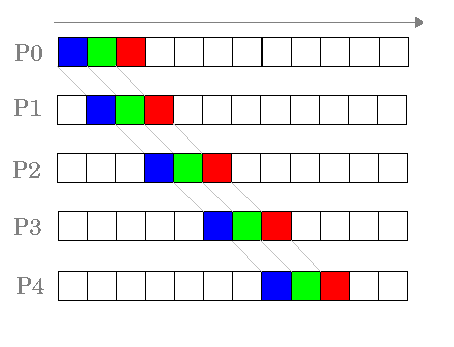
\includegraphics[width=0.45\linewidth]{images/modeles/definitions/chainseg}
%	\caption{\label{Figure: Chaine et segmentation}Structure de communication
%		d'une Chaîne Segmentée}
%	
%\end{figure}
%
%
%
%\subsubsection*{Pieuvre}
%
%Si une chaîne est trop sensible à l'accumulation des retards des processus,
%une alternative suffisamment efficace est l'implémentation d'une stratégie
%hybride, qui mélange à la fois un Arbre Plat ou Binomial et des chaînes
%segmentées. Cette stratégie, appelée \emph{pieuvre} (ou \emph{k-chain}
%en anglais \cite{Pjesivac-Grbovic05}, Figure \ref{Figure: k-chain}) utilise
%un petit \og coeur \fg{} en forme d'arbre plat ou binomial, dont
%les processus donnent à leur tour naissance à plusieurs chaînes. 
%
%%
%\begin{figure}[h]
%	\centering
%		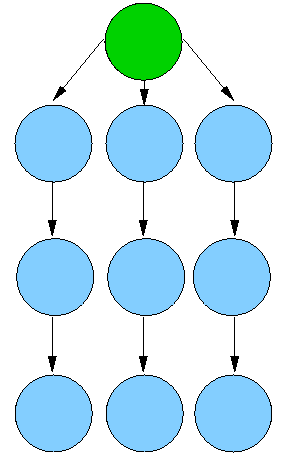
\includegraphics[width=0.25\linewidth]{images/modeles/definitions/bcastkchain}
%		
%	\caption{\label{Figure: k-chain}Structure de fonctionnement d'un arbre \emph{pieuvre}}
%	
%\end{figure}
%
%
%En conséquence, les chaînes formées sont plus courtes et plus nombreuses
%; les effets dus au retard d'un processus affectent seulement un groupe
%de processus, et le retard accumulé sera moins répandu dans les chaînes
%de diffusion. Ceci dit, un désavantage de cette stratégie par rapport
%à la Chaîne Segmentée classique est que le nombre de processus doit
%être suffisamment grand pour que l'accumulation des latences compense
%le coût initial des arbres de diffusion. Dans les expériences effectuées
%dans le cadre de ce travail, la performance de la pieuvre n'a pas
%pu dépasser celle de la chaîne segmentée, malgré un léger gain de
%performance par rapport à l'arbre binomial. Pour cette raison, et
%à cause de sa complexité, nous avons préféré l'étude de la chaîne
%segmentée, technique déjà utilisée pour la distribution de données
%à large échelle. 
%
%
%%\subsubsection*{Scatter/Collection}
%%
%%L'algorithme en arbre binomial est adéquat aux petits messages à cause
%%de son coût de latence logarithmique, tandis qu'un algorithme de type
%%Chaîne Segmentée peut s'avérer efficace pour les grands messages.
%%Cependant, l'algorithme en Chaîne Segmentée requiert une performance
%%uniforme de tous les processus, sinon sa performance est trop sujette
%%à des variations. 
%%
%%Une alternative plus sûre pour la diffusion de grands messages est
%%l'algorithme Scatter-Collection, proposé par Van de Geijn et \emph{al.}
%%\cite{Barnett96}. Dans cet algorithme, le message est d'abord partagé
%%entre les processus à l'aide d'une opération similaire à MPI\_Scatter
%%; ensuite, les données sont regroupées avec une opération similaire
%%à MPI\_Allgather. Le temps d'exécution est alors la somme du temps
%%d'exécution du \emph{Scatter} et du \emph{Allgather}. 
%%
%%En effet, Thakur \emph{et al.} \cite{Thakur03} utilisent cette technique
%%pour l'implémentation de MPI\_Bcast adaptée aux grands messages, où
%%un algorithme binomial est utilisé pour le \emph{Scatter} et un algorithme
%%en anneau pour le \emph{Allgather}.
%%
%%
%\subsubsection*{Segmentation et arbres de diffusion}
%
%Si dans certains cas la segmentation peut augmenter la performance
%de certaines stratégies de diffusion, cela ne s'applique pas à toutes
%les stratégies de communication. Par exemple, l'apport de l'utilisation
%conjointe de la segmentation de messages et des stratégies de broadcast
%en arbre Plat ou Binomial dépend surtout des paramètres de communication
%(\emph{L} et \emph{g}), une fois que ces stratégies obligent une interdépendance
%entre processus par rapport à la distribution des données. Pour mieux
%illustrer cette situation, la Figure \ref{Figure: Arbre Binomial et Segmentation}
%représentent le schéma de communication pour l'algorithme en arbre
%binomial avec $L=1$ et $g=1$. Nous observons que la structure de
%cet algorithme oblige un flux de données qui n'est pas adapté à l'enchaînement
%des communications, comme c'était le cas avec la chaîne segmentée
%\ref{Figure: Chaine et segmentation}. 
%
%
%
%\begin{figure}[t]
%	\centering
%		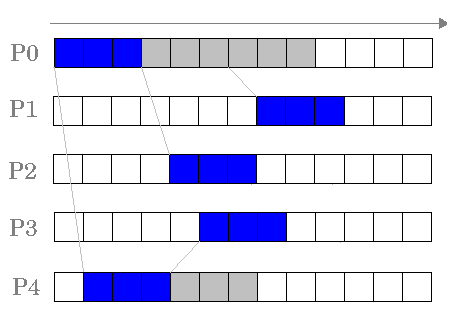
\includegraphics[width=0.45\linewidth]{images/modeles/definitions/binomialtrad} 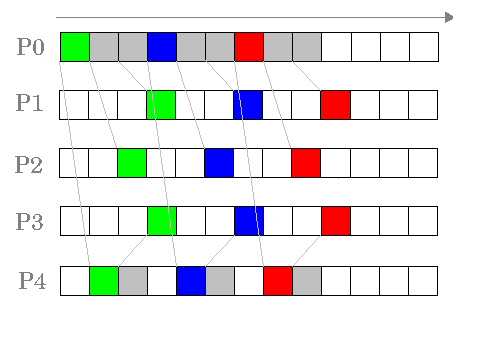
\includegraphics[width=0.45\linewidth]{images/modeles/definitions/binomialseg}
%	\caption{\label{Figure: Arbre Binomial et Segmentation}La stratégie en Arbre
%		Binomial sans et avec segmentation avec L=1 et g=1}
%	
%\end{figure}
%
%
%En effet, pour des valeurs de $g\geq L$, la chaîne segmentée est
%la forme optimale; seulement si $g\leq L$ les autres formes d'arbre
%deviennent plus intéressantes, car elles rendent possible le recouvrement
%de la latence de communication par des émissions successives.


\subsection{\label{sub:Broadcast_Practical}Validation des modèles}

Pour valider ces modèles de communication, nous avons choisi la comparaison
entre les prédictions des modèles et les résultats réels obtenus à
partir d'expérimentations sur différentes plates-formes réseaux. Pour
illustrer notre approche, nous avons comparé des implémentations de
MPI\_Bcast selon les stratégies Arbre Plat, Arbre Binomial et Chaîne
Segmentée. 
%Dans les prochaines pages nous présentons l'analyse des
%expérimentations effectuées sur chaque plate-forme réseau différente. 


\subsubsection*{Réseau Fast Ethernet}

Comme nous pouvons observer dans les Figures \ref{Figure:Comparison-Bcast_Flat_FEth},
\ref{Figure:Comparison-Bcast_Bin_FEth} et \ref{Figure:Comparison-Bcast-Chain_FEth},
les prédictions des trois stratégies d'implémentation représentent presque
fidèlement les résultats expérimentaux obtenus sur un cluster.
%le réseau Fast Ethernet. 

Plus spécifiquement, des différences entre les prédictions et les
valeurs réelles sont observées surtout dans le cas de la stratégie
en Arbre Binomial, où le temps mesuré pour l'envoi de petits messages
est plus élevé que celui prévu, et ne suit pas un comportement linéaire
par rapport à la taille des messages. Cette variation de performance,
observée aussi dans des expériences avec d'autres réseaux,
%le réseau Giga Ethernet,
a été l'objet d'analyses précédentes (cette discussion peut être retrouvée
dans les articles \cite{Steffenel04a} et \cite{Steffenel04c}) et dont l'origine des retards
est due à l'implémentation des politiques d'acquittement TCP sur Linux, qui retarde
des messages même si l'option \emph{socket} TCP\_NODELAY est activée. 

En effet, parfois un seul message
à chaque \emph{n} messages transmis n'est pas acquitté comme il le
faut. Cette défaillance du protocole d'acquittement induit un temps supplémentaire
nécessaire à la retransmission du message et à son acquittement.  

%
\begin{figure}[h]
	\centering
		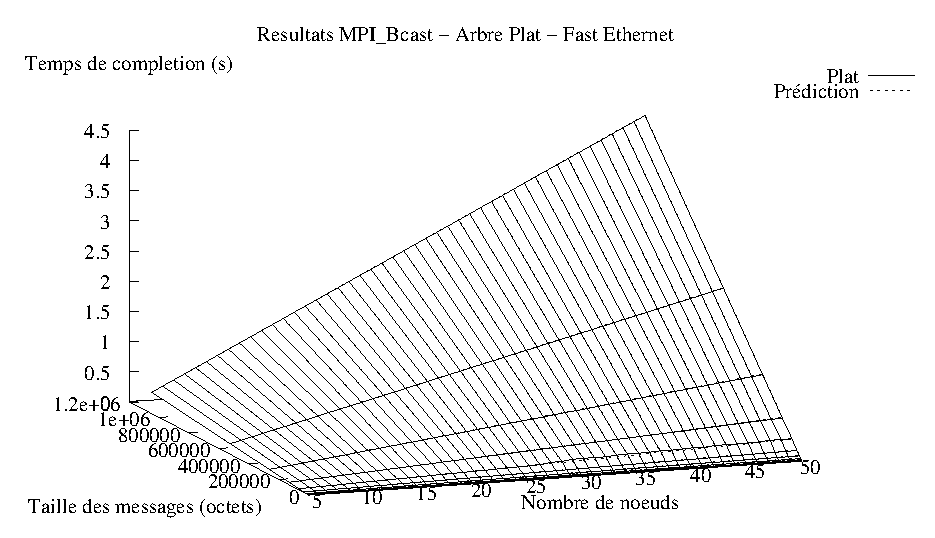
\includegraphics[width=0.6\linewidth]{images/modeles/FEth/Bcast/comp_Flat}
		
	\caption{\label{Figure:Comparison-Bcast_Flat_FEth}Les performances réelles
		et prédites pour l'Arbre Plat avec un réseau Fast Ethernet}
	
\end{figure}


%
\begin{figure}[h]
	\centering
		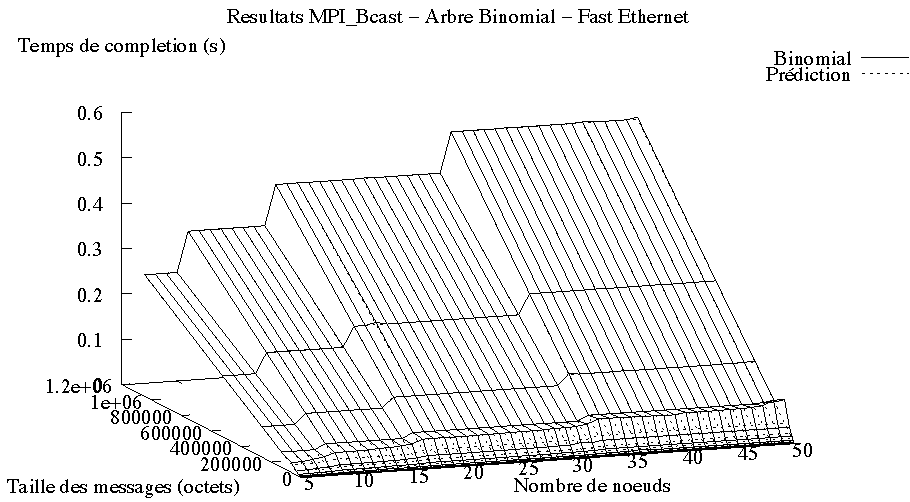
\includegraphics[width=0.6\linewidth]{images/modeles/FEth/Bcast/comp_Binomial}
	
	\caption{\label{Figure:Comparison-Bcast_Bin_FEth}Les performances réelles
		et prédites pour l'Arbre Binomial avec un réseau Fast Ethernet}
	
\end{figure}


%
\begin{figure}[h]
	\centering
		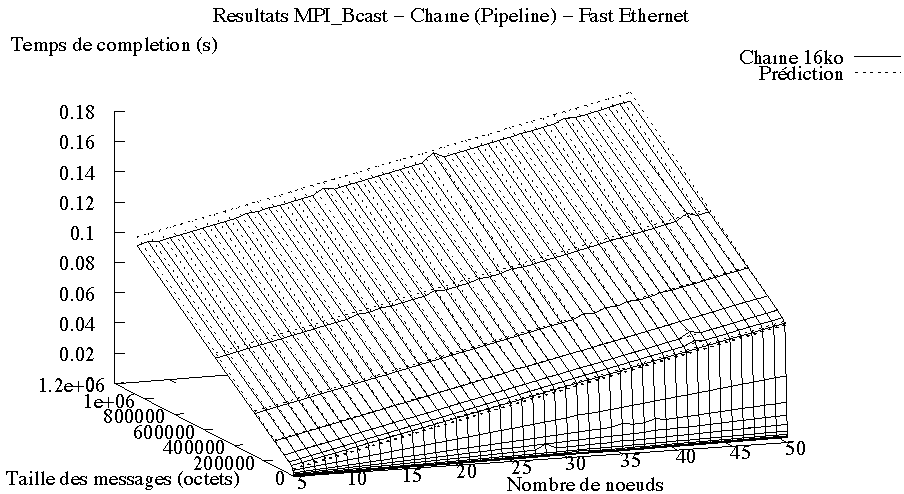
\includegraphics[width=0.6\linewidth]{images/modeles/FEth/Bcast/comp_Chain_16384}
	
	\caption{\label{Figure:Comparison-Bcast-Chain_FEth}Les performances réelles
		et prédites pour la Chaîne Segmentée avec un réseau Fast Ethernet}
	
\end{figure}

%
%Nous pouvons également observer dans la Figure \ref{Figure:Comparison-between-models Bcast FEth}
%le comportement des trois stratégies et leurs prédictions lorsque
%varie le nombre de processus. Nous observons que la stratégie en Arbre
%Plat est beaucoup moins performante que les deux autres stratégies,
%et sa performance décroît avec l'augmentation du nombre de processus
%communicants, alors que les autres stratégies sont beaucoup plus stables
%par rapport au nombre de processus. Cela est du au modèle de communication
%employé par la stratégie en Arbre Plat, qui la rend directement dépendante
%du nombre de processus et du surcoût d'envoi des messages (\emph{gap}).
%Les stratégies en Arbre Binomial et en Chaîne Segmentée sont moins
%sensibles à l'augmentation du nombre de processus car la première
%stratégie a un coût logarithmique, alors que la deuxième est linéairement
%dépendante de la latence, qui a une valeur bien plus réduite. 
%
%%
%\begin{figure}[h]
%	\centering
%		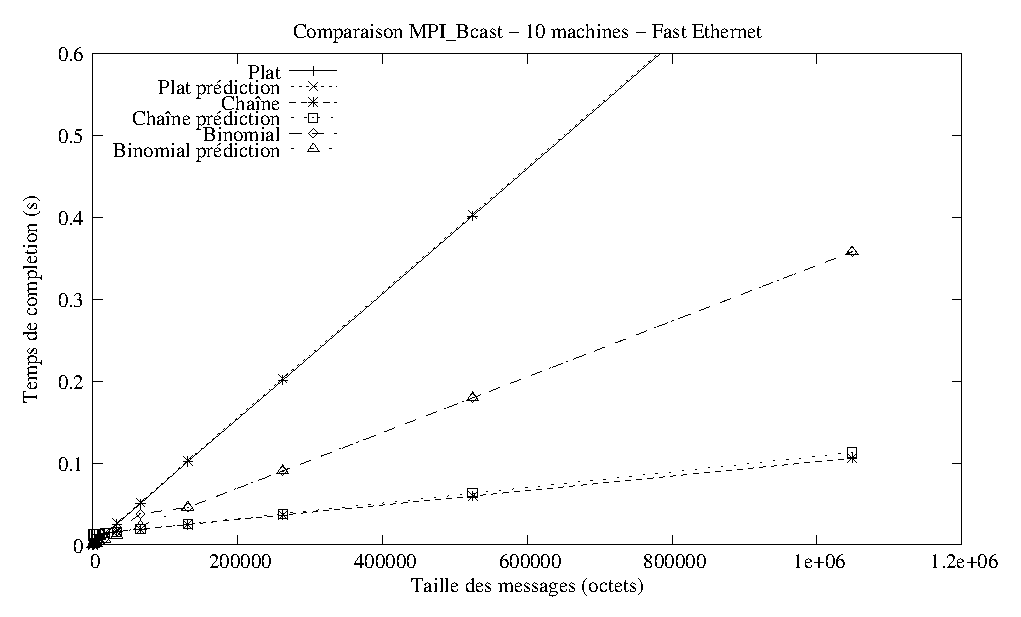
\includegraphics[width=0.6\linewidth]{images/modeles/FEth/Bcast/comp10}
%		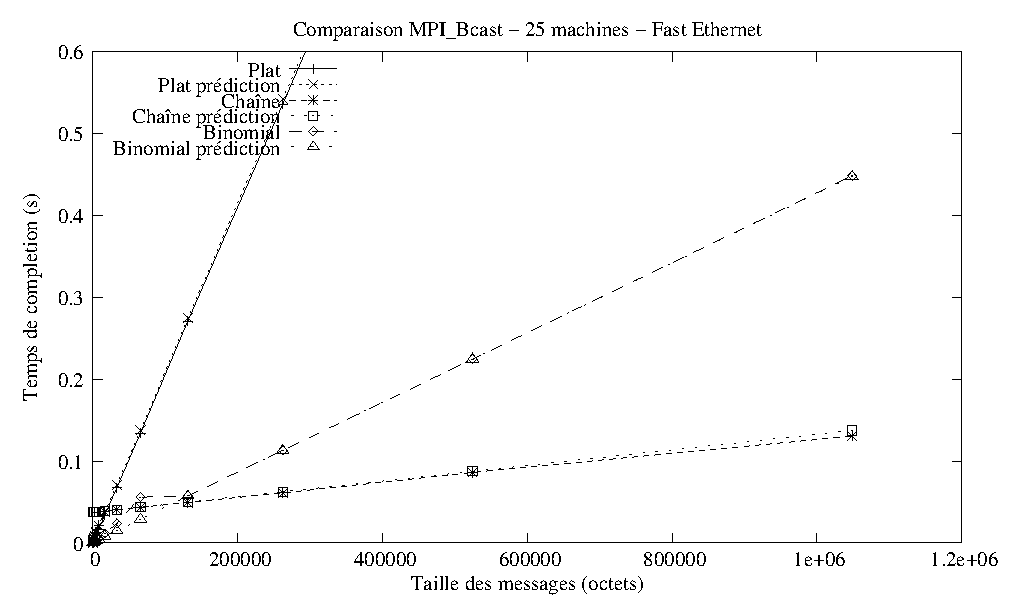
\includegraphics[width=0.6\linewidth]{images/modeles/FEth/Bcast/comp25}
%		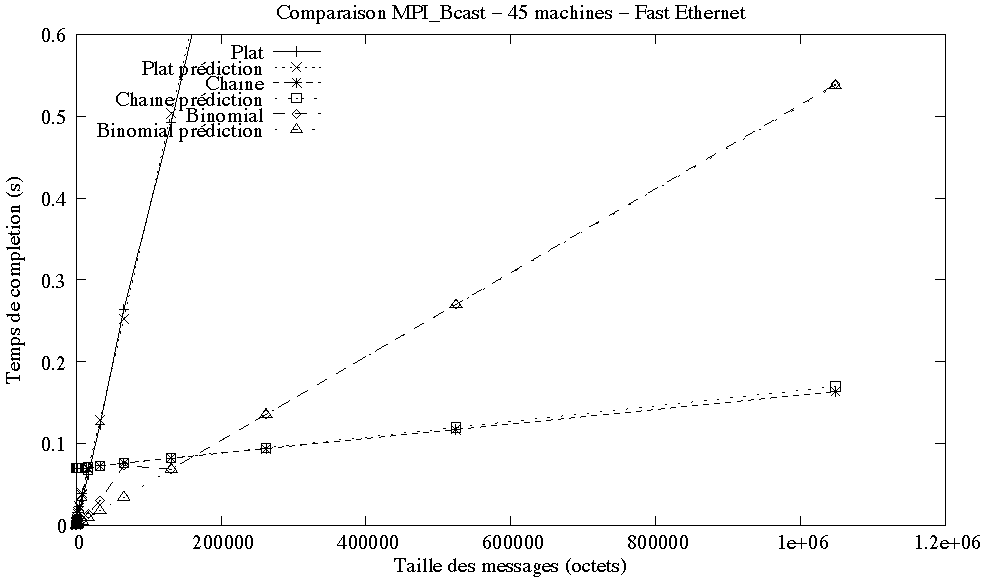
\includegraphics[width=0.6\linewidth]{images/modeles/FEth/Bcast/comp45}
%	
%	\caption{\label{Figure:Comparison-between-models Bcast FEth}Comparaison entre
%		les résultats réels et prédits pour des groupes de 10, 25 et 45 machines
%		dans un réseau Fast Ethernet}
%	
%\end{figure}


Les variations de performance observées dans le cas de la stratégie
en Arbre Binomial sont plus visibles dans la Figure \ref{Figure:Erreur-Bcast-FEth}.
Ici, nous observons que les résultats réels, normalement très proches
des prédictions (à une marge de 10\% maximum), s'écartent des prédictions
jusqu'à 90\% pour des messages autour de 128 Ko. Néanmoins, ces variations
affectent des communications où la différence absolue n'est que de
quelques millisecondes, ce qui n'empêche pas l'utilisation des modèles
de communication pour choisir la meilleure stratégie de communication. 

%
\begin{figure}[h]
	\centering
			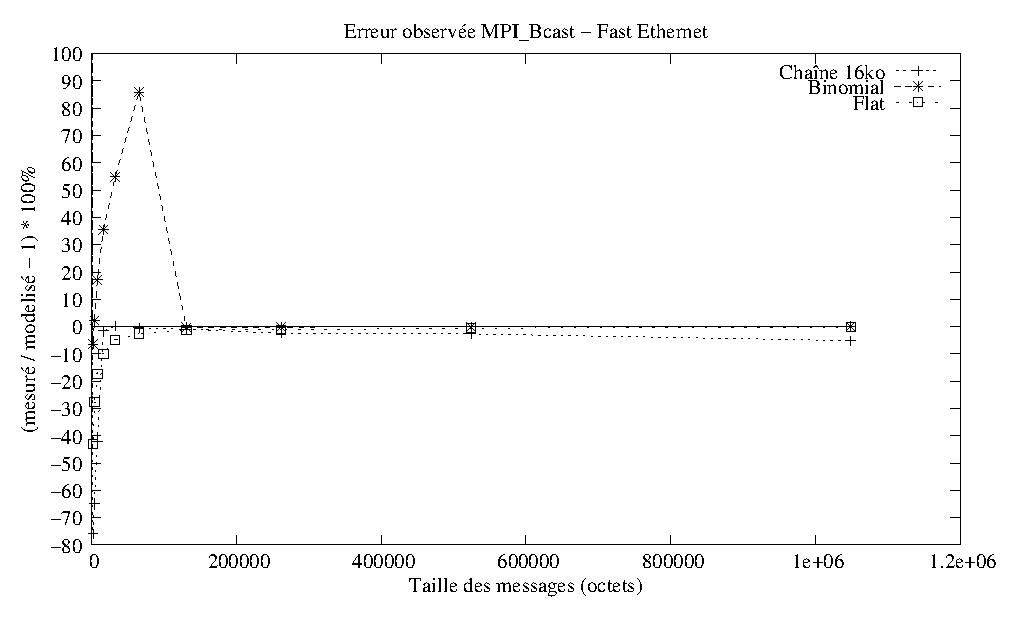
\includegraphics[width=0.6\linewidth]{images/modeles/FEth/Bcast/error}
		
	
	\caption{\label{Figure:Erreur-Bcast-FEth}L'erreur des prédictions par rapport
		aux valeurs mesurées, dans un réseau Fast Ethernet}
	
\end{figure}



%\subsubsection*{Réseau Giga Ethernet}
%
%Les résultats des expérimentations effectuées sur le réseau Giga Ethernet
%de la grappe \emph{Grid eXplorer} sont présentés dans les Figures
%\ref{Figure:Comparison-Bcast_Flat_GEth}, \ref{Figure:Comparison-Bcast_Bin_GEth}
%et \ref{Figure:Comparison-Bcast-Chain_GEth}. Si les prédictions pour
%la stratégie en Arbre Plat suivent fidèlement les résultats pratiques,
%nous observons des variations importantes dans les cas des stratégies
%en Arbre Binomial et en Chaîne Segmentée. Dans les deux cas, le temps
%des communications a subi une forte augmentation quand l'application
%utilise plus de 24 processus. Si l'origine de cette augmentation nécessite
%une investigation plus approfondie, nous considérons fortement la
%possibilité d'une surcharge du commutateur. En effet, la stratégie
%en Arbre Plat limite les communications à la capacité d'envoi du processus
%\emph{racine}, alors que les autres stratégies favorisent l'envoi
%simultané de messages par différents processus, ce qui peut surcharger
%le commutateur.
%
%%
%\begin{figure}[h]
%	\centering
%		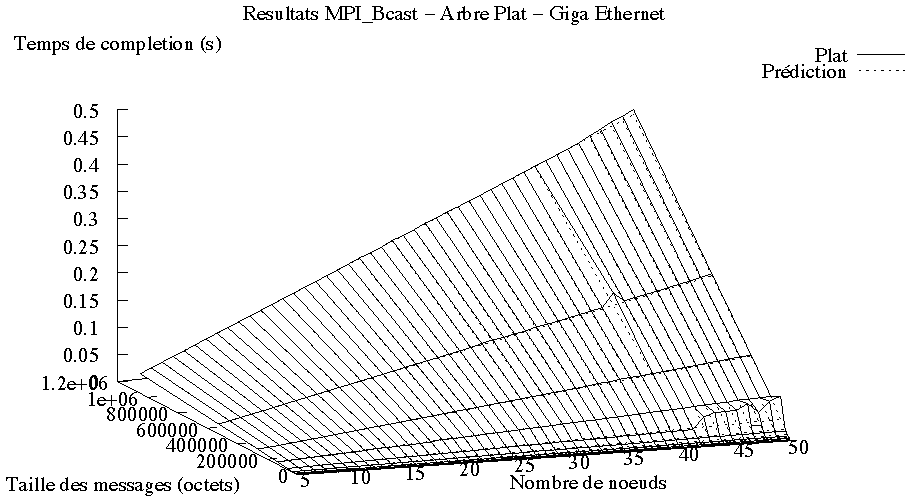
\includegraphics[width=0.6\linewidth]{images/modeles/GEth/Bcast/comp_Flat}
%	\caption{\label{Figure:Comparison-Bcast_Flat_GEth}Les performances réelles
%		et prédites pour l'Arbre Plat avec un réseau Giga Ethernet}
%	
%\end{figure}
%%
%\begin{figure}[h]
%	\centering
%		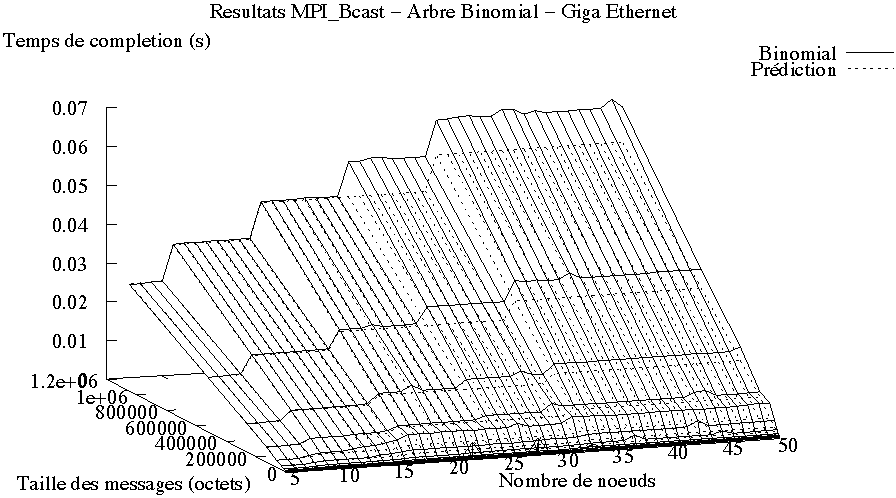
\includegraphics[width=0.6\linewidth]{images/modeles/GEth/Bcast/comp_Binomial}
%	
%	\caption{\label{Figure:Comparison-Bcast_Bin_GEth}Les performances réelles
%		et prédites pour l'Arbre Binomial avec un réseau Giga Ethernet}
%	
%\end{figure}
%
%
%%
%\begin{figure}[h]
%	\centering
%		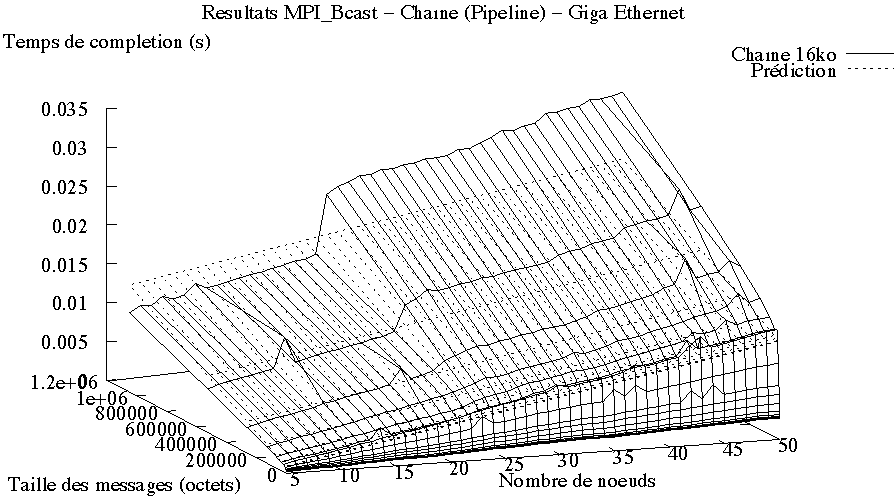
\includegraphics[width=0.6\linewidth]{images/modeles/GEth/Bcast/comp_Chain_16384}
%	
%	\caption{\label{Figure:Comparison-Bcast-Chain_GEth}Les performances réelles
%		et prédites pour la Chaîne Segmentée avec un réseau Giga Ethernet}
%	
%\end{figure}
%
%
%Toutefois, nous pouvons observer dans la Figure \ref{Figure:Comparison-between-models Bcast GEth}
%que si les prédictions ne correspondent pas exactement aux résultats
%réels, au moins elles suivent le comportement général des trois stratégies
%d'implémentation. Plus exactement, si nous considérons seulement le
%cas des 10 processus (et que par conséquent sont exemptés des effets
%dûs au commutateur), les prédictions sont très similaires aux résultats
%réels, comme atteste la Figure \ref{Figure:Comparison-between-models Bcast GEth}(a). 
%
%Dans tous les cas, nous observons que la stratégie en Arbre Plat est
%beaucoup moins performante que les deux autres stratégies, et que
%la Chaîne Segmentée présente la meilleure performance pour les grands
%messages (la meilleure stratégie pour l'envoi de petits messages dépend
%surtout du nombre de processus).
%
%%
%\begin{figure}[h]
%	\centering
%		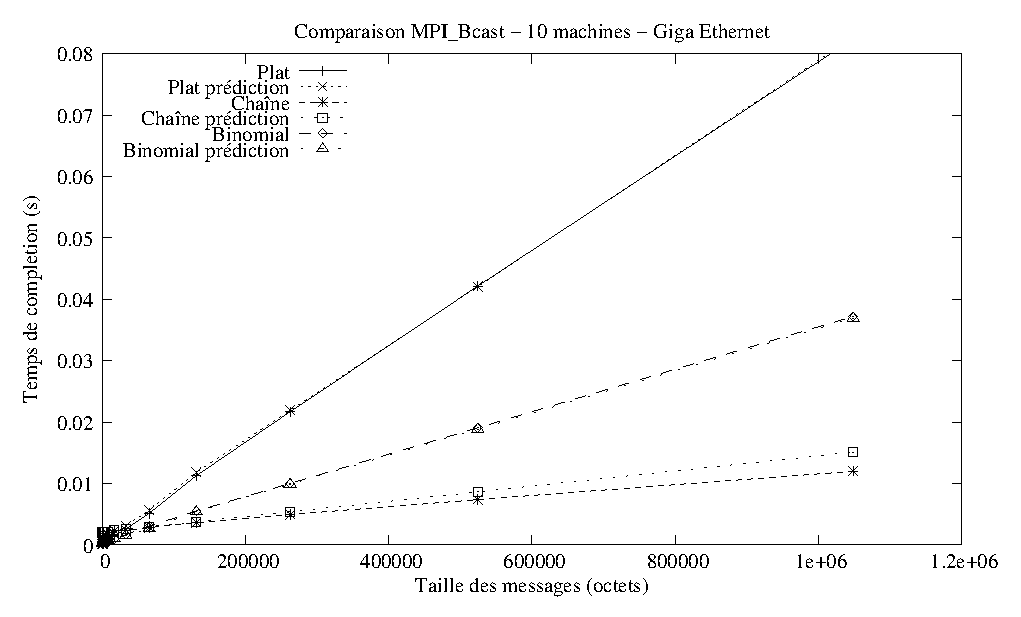
\includegraphics[width=0.6\linewidth]{images/modeles/GEth/Bcast/comp10}\\
%		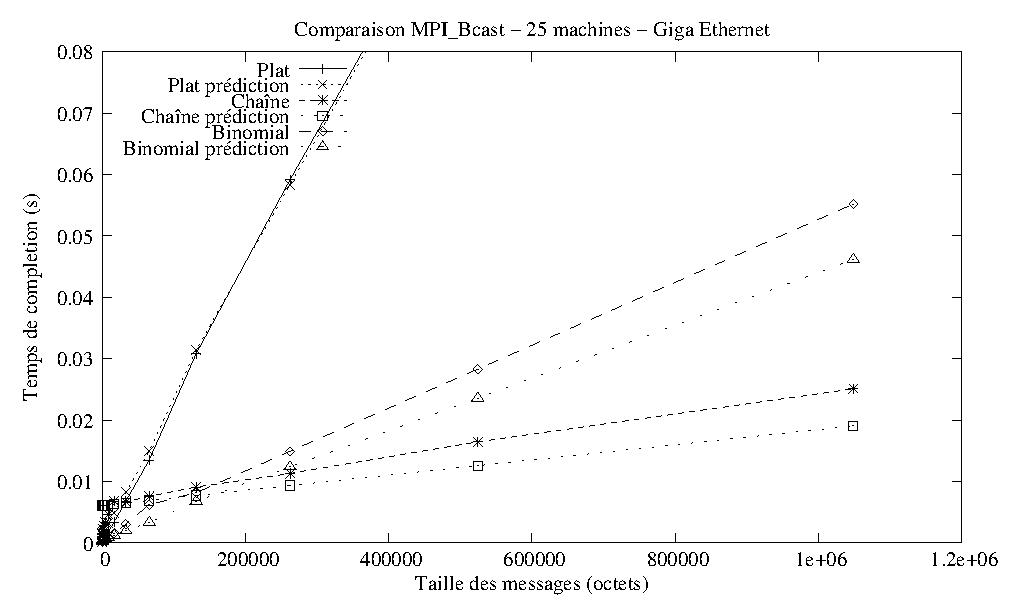
\includegraphics[width=0.6\linewidth]{images/modeles/GEth/Bcast/comp25}\\
%		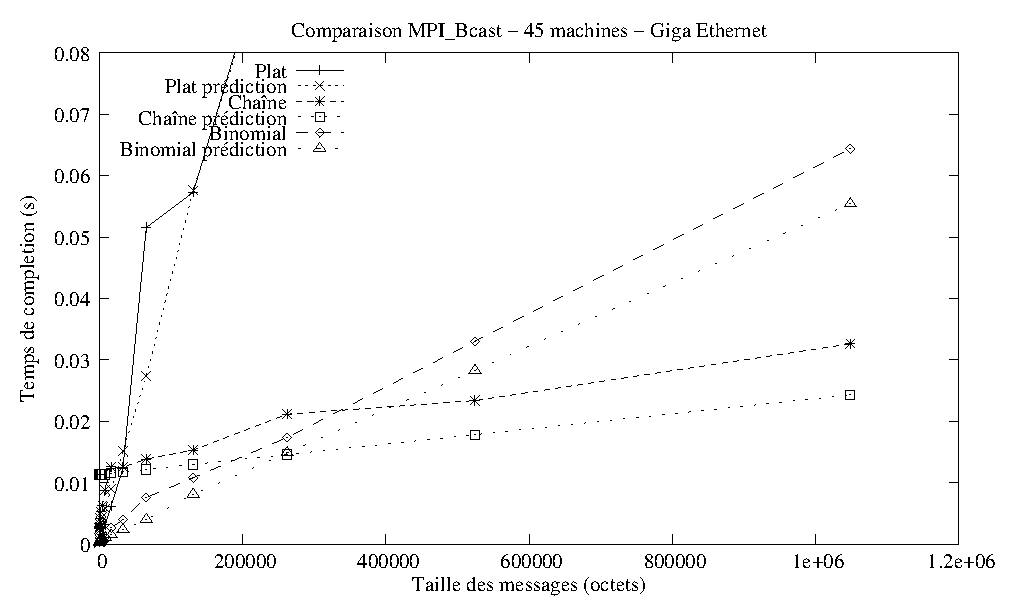
\includegraphics[width=0.6\linewidth]{images/modeles/GEth/Bcast/comp45}
%	\caption{\label{Figure:Comparison-between-models Bcast GEth}Comparaison entre
%		les résultats réels et prédits pour des groupes de 10, 25 et 45 machines
%		dans un réseau Giga Ethernet}
%	
%\end{figure}
%
%
%Étant donné que le surcout dû à la surcharge du commutateur est un
%facteur difficile à prédire, nous avons concentré l'analyse de l'erreur
%relative des prédictions au groupe de processus qui n'étaient pas
%sous l'influence du commutateur surchargé. Ainsi, nous pouvons observer
%dans la Figure \ref{Figure:Erreur_Bcast_GEth} que les prédictions
%sont suffisamment proches des résultats expérimentaux, avec une erreur
%généralement inférieure à 10\%. Nous pouvons aussi constater que l'approche
%en Arbre Binomial subit les mêmes variations déjà observées dans le
%cas du réseau Fast Ethernet avec des petits messages, ce qui corrobore
%l'hypothèse que l'implémentation du protocole TCP sous Linux occasionne
%arbitrairement des retards importants pour certains messages.
%
%%
%\begin{figure}[h]
%	\begin{centering}
%		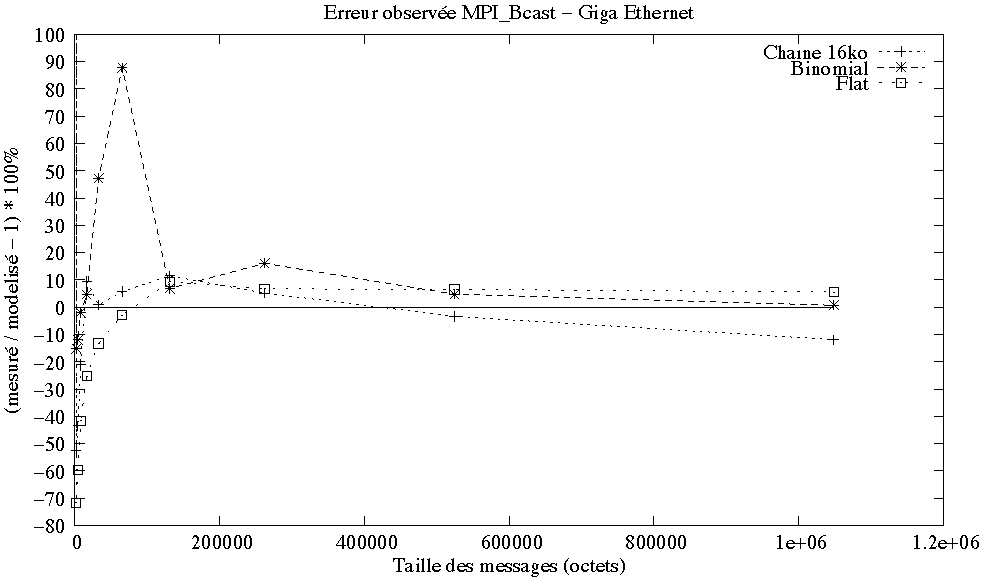
\includegraphics[width=0.6\linewidth]{images/modeles/GEth/Bcast/error}
%	\end{centering}
%	
%	\caption{\label{Figure:Erreur_Bcast_GEth}L'erreur des prédictions par rapport
%		aux valeurs mesurées, dans un réseau Giga Ethernet}
%	
%\end{figure}
%
%
%
%%\subsubsection*{Réseau Myrinet}
%%
%%
%%Les expériences conduites sur le réseau Myrinet de la grappe \emph{icluster-2}
%%sont présentées dans les Figures \ref{Figure:Comparison-Bcast_Flat_Myri},
%%\ref{Figure:Comparison-Bcast_Bin_Myri} et \ref{Figure:Comparison-Bcast-Chain_Myri}.
%%Similairement à ce qui a déjà été observé pour les réseaux Fast Ethernet
%%et Giga Ethernet, les modèles de communication des stratégies en Arbre
%%Plat et Arbre Binomial reproduisent fidèlement le comportement des
%%expériences pratiques. 
%%
%%%
%%\begin{figure}[h]
%%	\begin{centering}
%%		\begin{tabular}{c}
%%			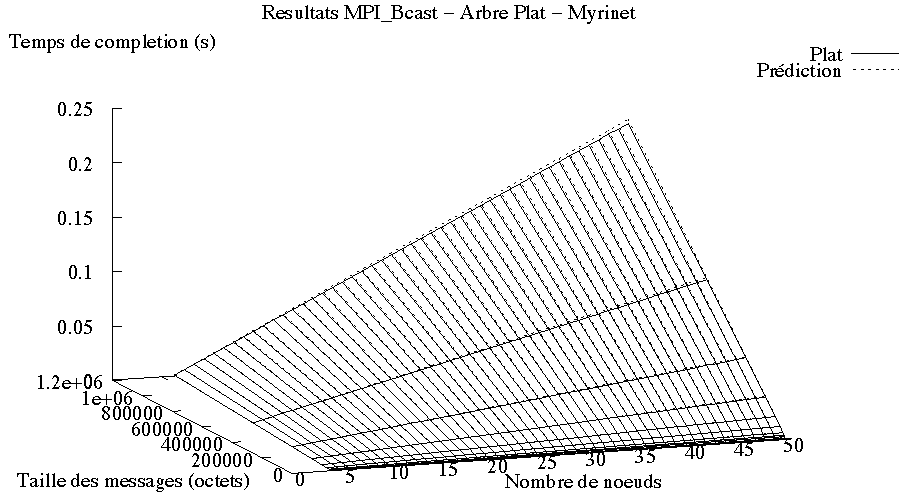
\includegraphics[width=0.6\linewidth]{images/modeles/Myrinet/Bcast/comp_Flat}\tabularnewline
%%		\end{tabular}\vspace{-0.5cm}
%%		\par\end{centering}
%%	
%%	\caption{\label{Figure:Comparison-Bcast_Flat_Myri}Les performances réelles
%%		et prédites pour l'Arbre Plat avec un réseau Myrinet}
%%	
%%\end{figure}
%%
%%
%%%
%%\begin{figure}[h]
%%	\begin{centering}
%%		\begin{tabular}{c}
%%			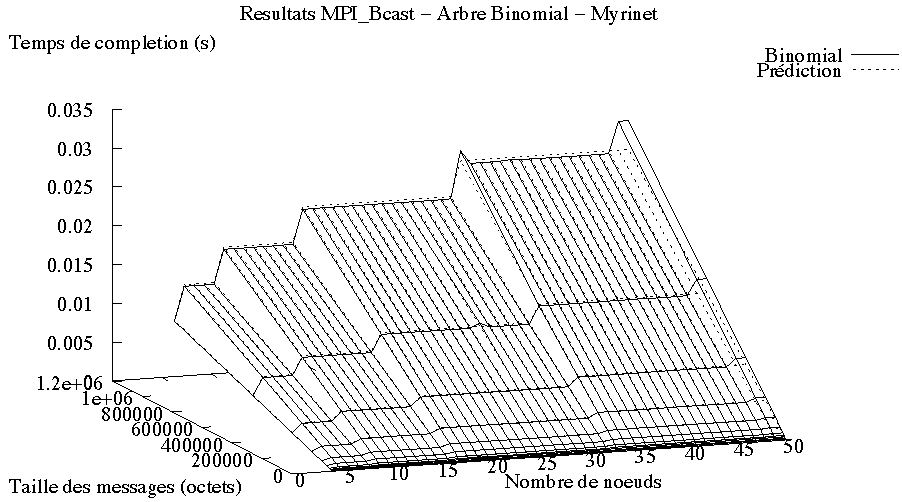
\includegraphics[width=0.6\linewidth]{images/modeles/Myrinet/Bcast/comp_Binomial}\tabularnewline
%%		\end{tabular}\vspace{-0.5cm}
%%		\par\end{centering}
%%	
%%	\caption{\label{Figure:Comparison-Bcast_Bin_Myri}Les performances réelles
%%		et prédites pour l'Arbre Binomial avec un réseau Myrinet}
%%	
%%\end{figure}
%%
%%
%%%
%%\begin{figure}[h]
%%	\begin{centering}
%%		\begin{tabular}{c}
%%			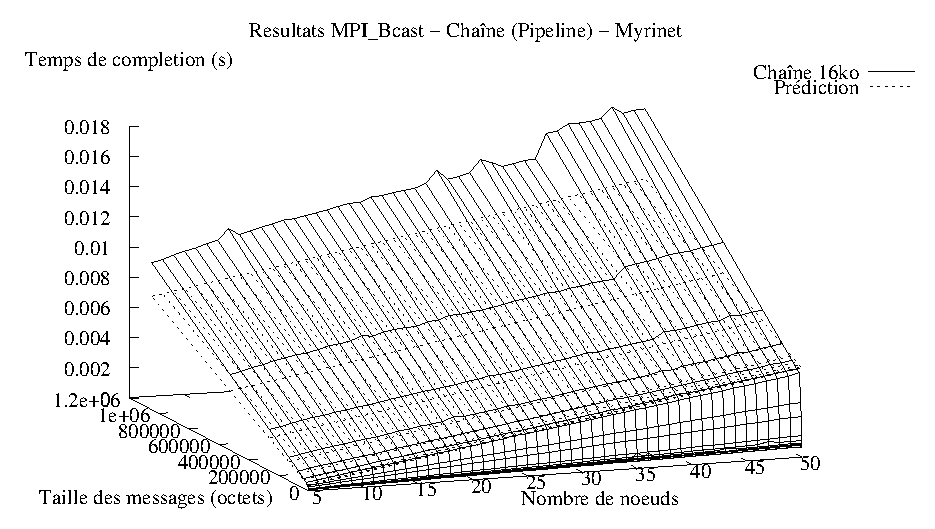
\includegraphics[width=0.6\linewidth]{images/modeles/Myrinet/Bcast/comp_Chain_16384}\tabularnewline
%%		\end{tabular}\vspace{-0.5cm}
%%		\par\end{centering}
%%	
%%	\caption{\label{Figure:Comparison-Bcast-Chain_Myri}Les performances réelles
%%		et prédites pour la Chaîne Segmentée avec un réseau Myrinet}
%%	
%%\end{figure}
%%
%%
%%Dans le cas de la Chaîne Segmentée toutefois les prédictions sous-estiment
%%le temps nécessaire à l'exécution du broadcast. Nous croyons que l'erreur
%%observée est liée au coût de la manipulation des segments. Ce coût,
%%qui normalement représente une petite partie du temps total d'exécution,
%%devient plus important quand l'environnement réseau utilisé est suffisamment
%%rapide, à l'exemple du réseau Myrinet, où la latence et le \emph{gap}
%%sont très faibles par rapport aux autres architectures réseau utilisées.
%%Pour vérifier si cette erreur est réellement due à la manipulation
%%des segments et pas au mauvais choix du segment, nous avons effectué
%%l'expérience avec d'autres tailles de segment, 32Ko et 64Ko (Figures
%%\ref{Figure:Comparison-Bcast-Chain_Myri_outrosseg}a et \ref{Figure:Comparison-Bcast-Chain_Myri_outrosseg}b).
%%Celles ci montrent d'un côté que le surcoût par rapport à la prédiction
%%reste importante, mais aussi que l'utilisation de segments plus grands
%%n'a pas permis la réduction du temps de communication.
%%
%%%
%%\begin{figure}[h]
%%	\begin{centering}
%%		\begin{tabular}{c}
%%			\subfigure[Chaîne segmentée avec 32Ko]{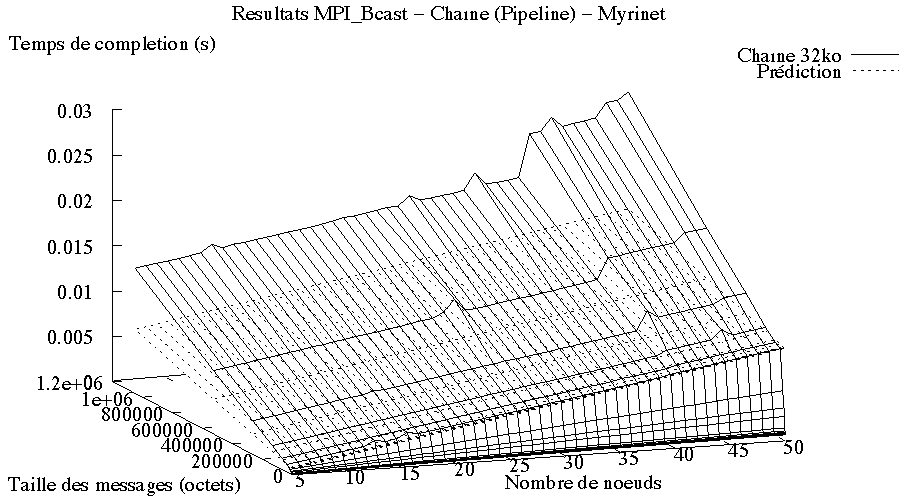
\includegraphics[width=0.6\linewidth]{images/modeles/Myrinet/Bcast/comp_Chain_32768}}\tabularnewline
%%		\end{tabular}\vspace{-0.5cm}\\
%%		\begin{tabular}{c}
%%			\subfigure[Chaîne segmentée avec 64Ko]{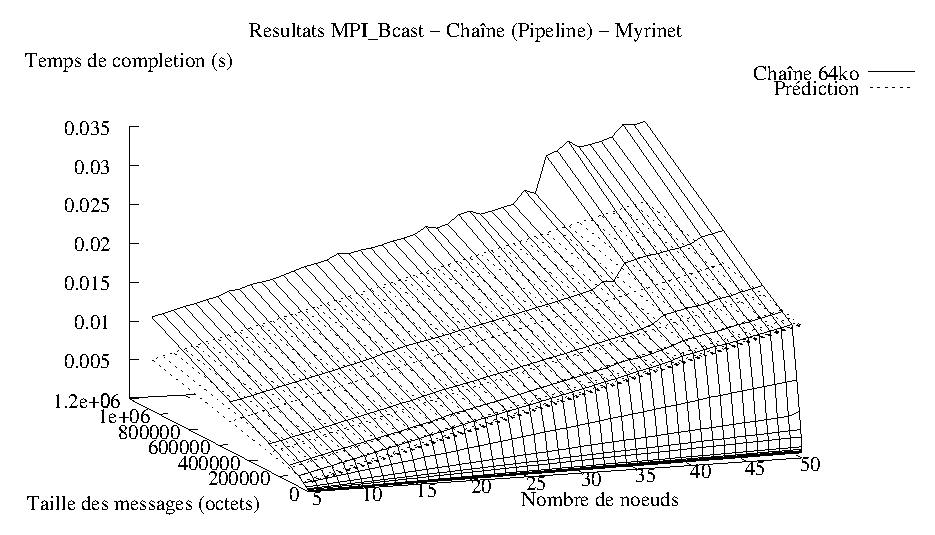
\includegraphics[width=0.6\linewidth]{images/modeles/Myrinet/Bcast/comp_Chain_65536}}\tabularnewline
%%		\end{tabular}\vspace{-0.5cm}
%%		\par\end{centering}
%%	
%%	\caption{\label{Figure:Comparison-Bcast-Chain_Myri_outrosseg}Les performances
%%		réelles et prédites pour la Chaîne Segmentée sur un réseau Myrinet
%%		avec différentes tailles de segment}
%%	
%%\end{figure}
%%
%%
%%Bien que les prédictions pour la Chaîne Segmentée ont une marge d'erreur
%%plus importante, nous pouvons observer dans la Figure \ref{Figure:Comparison-between-models Bcast Myri}
%%que les prédictions de cette stratégie sont encore suffisamment proches
%%pour permettre le choix de la meilleure stratégie à utiliser. Cependant,
%%avec le développement et la démocratisation d'architectures réseau
%%plus rapides, on peut envisager l'intégration de ce coût aux modèles
%%de communication, à l'exemple de l'approche proposée pour le patron
%%de communication \emph{Plusieurs vers Plusieurs Personnalisé}, décrite
%%dans la section \ref{sec:Alltoall}.
%%
%%%
%%\begin{figure}[h]
%%	\begin{centering}
%%		\vspace{-0.5cm}\begin{tabular}{c}
%%			\subfigure[10 machines]{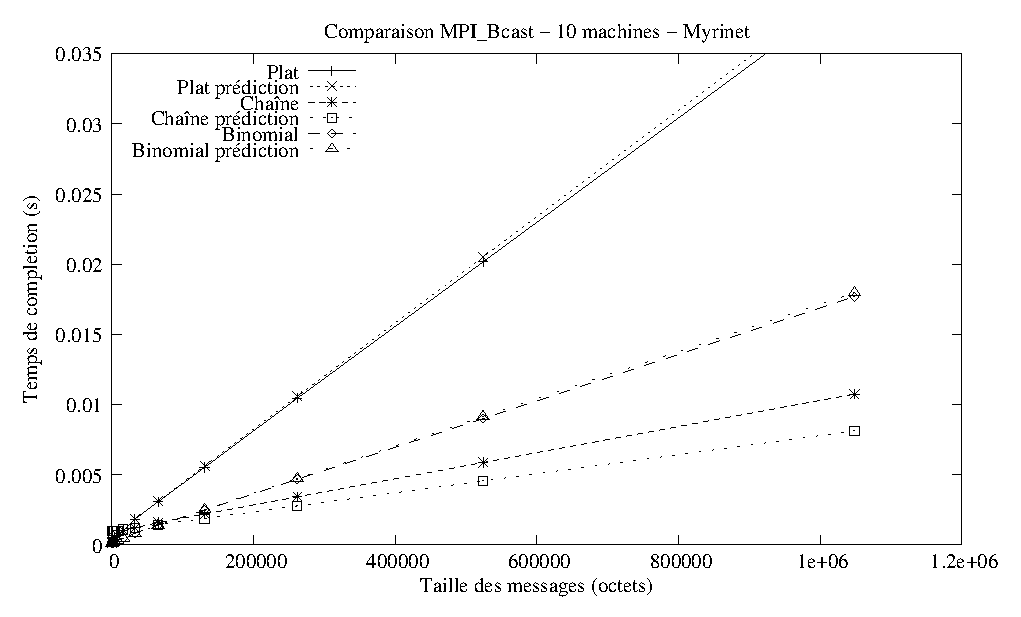
\includegraphics[width=0.6\linewidth]{images/modeles/Myrinet/Bcast/comp10}}\tabularnewline
%%		\end{tabular}\\
%%		\vspace{-0.5cm}
%%		\par\end{centering}
%%	
%%	\begin{centering}
%%		\begin{tabular}{c}
%%			\subfigure[25 machines]{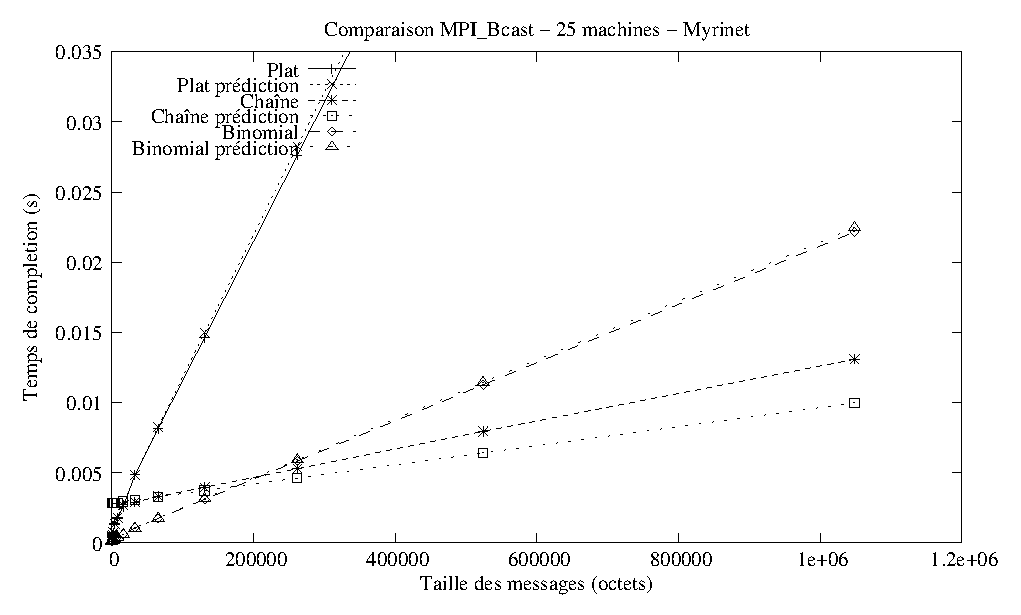
\includegraphics[width=0.6\linewidth]{images/modeles/Myrinet/Bcast/comp25}}\tabularnewline
%%		\end{tabular}\vspace{-0.5cm}
%%		\par\end{centering}
%%	
%%	\begin{centering}
%%		\begin{tabular}{c}
%%			\subfigure[45 machines]{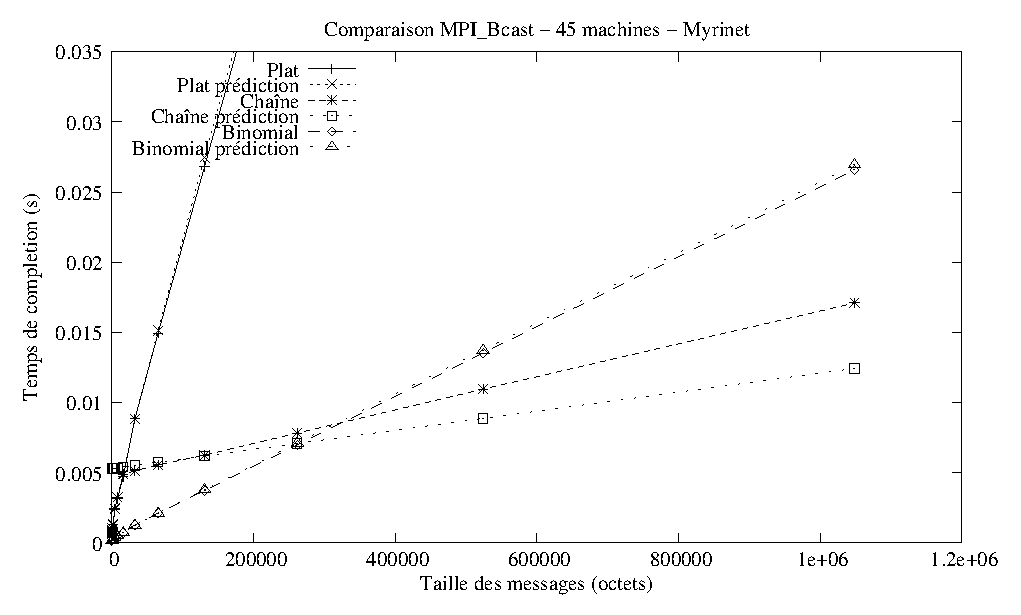
\includegraphics[width=0.6\linewidth]{images/modeles/Myrinet/Bcast/comp45}}\tabularnewline
%%		\end{tabular}\vspace{-0.5cm}
%%		\par\end{centering}
%%	
%%	\caption{\label{Figure:Comparison-between-models Bcast Myri}Comparaison entre
%%		les résultats réels et prédits pour des groupes de 10, 25 et 45 machines
%%		dans un réseau Myrinet}
%%	
%%\end{figure}
%%
%%
%%L'impact du coût dû à la segmentation des messages sur l'approche
%%Chaîne Segmentée peut être mieux observé à travers l'analyse de l'erreur
%%présentée dans la Figure \ref{Figure:Erreur Bcast Myri}. Alors que
%%les autres stratégies de communication ont une erreur insignifiante,
%%l'erreur des prédictions pour la Chaîne Segmentée peut dépasser les
%%30\% selon la taille de segment utilisée, mais se stabilise avec l'augmentation
%%de la taille des messages envoyés.
%%
%%%
%%\begin{figure}[h]
%%	\begin{centering}
%%		\begin{tabular}{c}
%%			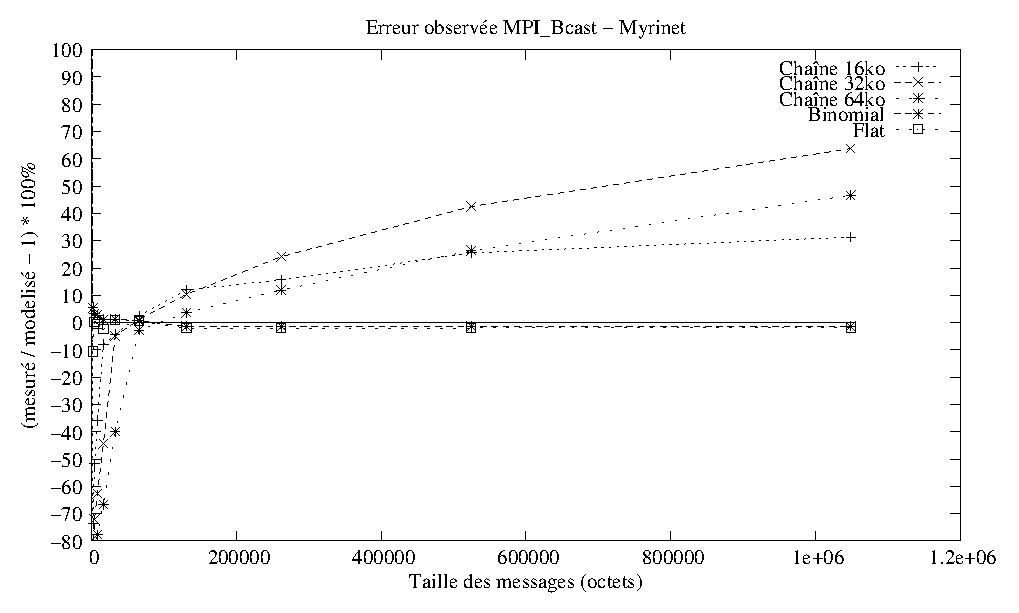
\includegraphics[width=0.6\linewidth]{images/modeles/Myrinet/Bcast/error}\tabularnewline
%%		\end{tabular}\vspace{-0.5cm}
%%		\par\end{centering}
%%	
%%	\caption{\label{Figure:Erreur Bcast Myri}L'erreur des prédictions par rapport
%%		aux valeurs mesurées, dans un réseau Myrinet}
%%	
%%\end{figure}
%%
%%
%%
%%
%%
%%
%%
%\section{Découverte de Topologie et Classification des Ressources \label{sec:reseaux-topo}}
%
%La connaissance de la topologie du réseau est un atout indispensable
%pour la distribution efficace des applications, et pour l'optimisation
%des communications entre les processus parallèles. Une utilisation
%de la connaissance de la topologie est le placement des processus
%parallèles, selon leur nombre et leurs besoins en ressources de calcul
%\cite{Park03}. Cependant, quand les ressources nécessaires ne sont
%plus contraintes à une seule grappe, le simple placement des processus
%ne suffit pas pour garantir la performance de l'application, spécialement
%si les applications échangent intensivement des messages.
%
%Afin d'assurer une performance de communication compatible avec le
%nombre de ressources employées, nous nous intéressons à la découverte
%de topologie comme un outil pour augmenter la connaissance du réseau,
%afin de faciliter la construction des primitives de communication
%collective adaptées aux environnements de type grille de calcul. Puisque
%les environnements de grille sont intrinsèquement hétérogènes et comptent
%un nombre important de composants, l'optimisation des communications
%collectives ne permet plus l'utilisation de stratégies exhaustives
%comme celles proposées par Bhat \cite{Bhat03} ou Vadhiyar\cite{Vadhiyar00}.
%En effet, ces propositions considèrent soit la génération d'arbres
%de communication à partir des données d'interconnexion de tous les
%noeuds, soit l'expérimentation pratique pour déterminer les meilleurs
%paramètres d'utilisation. 
%
%%Une solution adoptée par plusieurs auteurs pour réduire la complexité
%%des optimisations est la sous-division du réseau en différentes couches
%%de communication. Ainsi, l'approche la plus simple est d'établir une
%%séparation entre les communications de courte et longue distance,
%%ce qui permet, par exemple, l'optimisation des communications entre
%%deux grappes distantes, normalement plus lentes que les communications
%%à l'intérieur des grappes. Un autre avantage de cette stratégie est
%%que les ressources à l'intérieur d'une grappe sont normalement homogènes,
%%ce qui facilite la modélisation des communications et par conséquent,
%%réduit la complexité des optimisations. Quelques exemples de cette
%%approche en \og deux couches \fg{} sont les systèmes ECO \cite{Lowekamp96,Lowekamp00}
%%et MagPIe \cite{Kielmann99b}. On observe toutefois que le découpage en plus de deux couches n'est pas une
%%pratique courante, malgré les résultats présentés par Karonis \cite{Karonis00,Karonis02}
%%qui démontrent la possibilité d'augmenter la performance des communications
%%collectives par l'utilisation de plusieurs couches de communications,
%%adaptées à la topologie du réseau et au coût des communications à
%%l'intérieur des grappes. 
%
%L'approche suivie par ce travail est celle des multiples couches de
%communication. En effet, nous utilisons des outils de découverte de
%topologie pour identifier au milieu de la grappe des \og îlots d'homogénéité \fg{}
%ou \emph{grappes logiques}. Associée à l'obtention de paramètres précis
%d'interconnexion du réseau, la découverte de topologie permet alors
%le découpage virtuel du réseau et la réorganisation des couches de
%communication pour augmenter l'efficacité des communications collectives.
%
%
%\subsection{\label{sub:Topologie-recherch=0000E9e}Caractéristiques recherchées}
%
%Nous nous intéressons à la découverte automatique de la topologie
%effective du réseau, en particulier les temps de communications entre
%les noeuds au niveau applicatif, et non à une vue précise et détaillée
%du réseau tel que le schéma de câblage physique ou le matériel de
%routage. Notre but est de permettre le regroupement des noeuds connectivement
%proches en îlots d'homogénéité (des grappes logiques). Dû à la diversité
%des patrons de communication, les opérations de communication collective
%ne sont pas nécessairement structurées comme des arbres avec une racine
%unique ; dans ce cas-là la connaissance des performances du réseau
%de bout en bout (\emph{end-to-end}) entre tous les noeuds est nécessaire.
%À cela s'ajoute le besoin de connaissance des performances au niveau
%de l'application, notamment entre processus distribués sur les
%noeuds de la grille.
%
%Par conséquent, la découverte de topologie dans le cadre de notre
%travail doit satisfaire les trois contraintes suivantes :
%
%\begin{description}
%\item [{Précision~au~niveau~de~l'application.}] L'environnement de
%l'application comporte normalement des services qui peuvent influencer
%la connectivité entre les noeuds. L'outil de découverte de topologie
%doit s'adapter à de tels environnements, et délivrer des informations
%adaptées à l'application. 
%\item [{Minimisation~du~nombre~de~mesures.}] Dû au grand nombre de
%noeuds qui composent une grille, la réalisation des tests de bout-en-bout
%entre tous les noeuds s'avère une tâche longue et intrusive. Afin
%de réduire les perturbations induites sur la grille, il faut limiter
%le nombre de tests. Par exemple, il suffit de mesurer la connectivité
%entre une paire de machines pour déduire celle de toutes les machines
%(similaires) sur un réseau local. 
%\item [{Exhaustivité.}] Pour toutes paires de machines, si aucun test direct
%n'est réalisé entre elles, le système doit pouvoir estimer leur connectivité
%par agrégation d'autres tests.
%\end{description}
%
%
%
%
%\subsection{Découverte de topologie et la structure du réseau}
%
%Le modèle de réseau OSI (\emph{Open Systems Interconnection} - interconnexion
%de systèmes ouverts) est constitué de sept couches. % % (cf. Figure \ref{Figure: Mod=0000E8le OSI}).
%Chaque couche offre une vision différente du réseau, donc le niveau
%considéré pour la découverte du réseau influe à la fois la topologie,
%la façon de la découvrir et les informations recueillies. Généralement,
%les niveaux 2 et 3 sont les plus couramment utilisés pour la découverte
%de topologie. 
%%La couche 2 est nommée "liaison de données", et correspond
%%aux protocoles spécifiques de chaque environnement réseau, par exemple,
%%le protocole Ethernet. Par contre, la couche 3, nommée "réseau",
%%correspond aux protocoles tels que le protocole internet (Internet
%%Protocol - IP). La couche 2 est plus proche des liens physiques que
%%la couche réseau et peut être utilisée pour obtenir des informations
%%à propos des routeurs non disponibles depuis le niveau 3. En revanche,
%%la couche 3 est plus proche de la vision que les applications ont
%%du réseau. 
%
%Il existent toutefois des situations où, selon les spécificités de l'application,
%il faut regarder les couches supérieures pour mieux représenter la
%connectivité entre les noeuds et/ou les processus. Il est donc nécessaire de tenir compte
%de tels mécanismes lors de l'établissement de méthodes de cartographie
%automatique du réseau, et la façon la plus fiable est d'utiliser directement
%les couches supérieures du modèle OSI pour obtenir la topologie effective
%du réseau, telle comme elle est perçue par l'application.
%
%Dans les prochaines sections nous présentons quelques approches utilisées pour la découverte de topologie, suivies d'une analyse de
%leurs avantages et inconvénients par rapport à nos objectifs. 
%
%
%\subsubsection{Topologie fournie par l'utilisateur}
%
%Certains outils et bibliothèques de communication adaptés aux environnements
%de grille (\emph{grid-aware}) organisent leurs communications à partir
%des informations de topologie fournies par l'utilisateur, comme dans
%le cas de MagPIe \cite{Kielmann99b} et MPICH-G2 \cite{Karonis03}. 
%
%Malgré sa simplicité, les topologies fondées sur la localité
%des machines ne sont pas suffisantes pour garantir la précision des
%modèles de communication et en particulier la construction de communications
%à plusieurs niveaux. Plus exactement, des paramètres d'évaluation
%de type "sous-réseau IP" ne peuvent pas représenter la topologie
%effective du réseau, et par conséquent, peuvent cacher des hétérogénéités
%qui ne sont alors pas prises en compte par les modèles de communication. 
%
%Si les informations sur la topologie ne sont pas adaptées à la modélisation
%des communications collectives, cela n'exclut pas l'utilisation de
%données de localisation pour orienter la découverte de la topologie,
%qui doit néanmoins extraire des informations qui représentent les
%interconnexions effectives du réseau ou de la grille.
%
%
%\subsubsection{Protocoles de gestion du réseau - SNMP}
%
%La couche 2 du modèle OSI est celle qui définit les réseaux locaux
%(LAN). Il serait donc possible de consulter directement les composants
%du réseau en utilisant le protocole SNMP (\emph{Simple Network Management
%Protocol} - protocole simple de gestion du réseau \cite{Bierman00}) et d'en extraire des informations topologiques.
%Ainsi, plusieurs travaux comme ceux de Bejerano \cite{Bejerano03}
%et Breitbart \cite{Breitbart00} utilisent SNMP pour construire la
%topologie des réseaux.
%
%Malheureusement, pour que cette approche soit efficace, il faut que
%les administrateurs configurent correctement les dispositifs réseau
%et permettent l'accès à ces informations. En effet, la plupart des requêtes SNMP sont bloquées pour raison de sécurité. Effectivement, il est rare d'obtenir
%le droit d'utiliser SNMP sur les réseaux d'organisations dont on ne
%fait pas partie. Même si les plates-formes classiques de grilles impliquent
%le plus souvent plusieurs organisations bien établies telles que des
%universités, obtenir l'autorisation d'effectuer des opérations non
%classiques telles que l'accès aux protocoles de la couche liaison
%peut devenir très coûteuse en temps et en efforts en raison de facteurs
%humains. 
%
%
%\subsubsection{Méthodes tomographiques }
%
%La tomographie est une méthode utilisée par exemple en imagerie médicale
%et consistant à reconstruire une vision tridimensionnelle d'un objet
%à partir de plusieurs vues bidimensionnelles. De manière comparable,
%différentes solutions existent pour reconstruire la topologie du réseau
%à partir d'informations collectées depuis différentes machines. Ces
%méthodes diffèrent principalement par la façon de collecter les visions
%locales de chaque machine. 
%
%	\subsubsection*{ping}
%	Le programme \emph{ping} est traditionnellement utilisé pour mesurer la connectivité et le
%	temps d'aller-retour (\emph{Round Trip Time} - RTT) d'un paquet entre
%	deux hôtes sur le réseau. Ce programme exploite l'utilisation des messages de service ICMP, dont les valeurs obtenues sont parfois trop éloignées des paramètres au niveau des applications et donc peu utiles pour les modèles de performance.
%	\subsubsection*{traceroute}
%	L'outil \emph{traceroute} traditionnement exploite un autre type de message de services ICMP, celui du TTL (time-to-live) expiré. Traceroute est largement utilisé par certains projets de cartographie automatique tels que TopoMon \cite{Burger02} et GIAS
%	\cite{Li01}, que l'utilisent pour déterminer les interactions de
%	flux de données à travers l'analyse des routes partagées entre différents
%	noeuds. Tout comme \textit{ping}, les résultats obtenus avec traceroute sont parfois très eloignés de ceux observés au niveau des applications. 
%	\subsubsection*{NWS}
%	Le Network Weather Service \cite{Wolski97} est un système distribué basé sur des capteurs logiciels
%	permettant de regrouper des informations sur l'état actuel du réseau
%	et des machines d'une plate-forme. Il est ainsi possible d'obtenir
%	le débit et la latence de chaque lien TCP reliant deux hôtes abritant
%	des capteurs NWS. De même, la charge processeur, les espaces mémoire
%	et disque disponibles ou le nombre de processeurs de chaque hôte peuvent
%	être mesurés. 
%	
%	NWS peut mesurer les performances en termes de bande passante et latence
%	pour tout lien TCP/IP entre deux de ses capteurs. La latence est définie
%	par le temps d'aller-retour (\emph{Round-Trip Time}) d'un paquet de
%	très petite taille : la machine souhaitant mesurer la latence chronomètre
%	le temps nécessaire pour que la machine cible lui renvoie le paquet
%	de quatre octets qu'elle lui a envoyé, selon Figure \ref{fig:NWS}. 
%	
%	%
%	\begin{figure}[h]
%		\begin{centering}
%			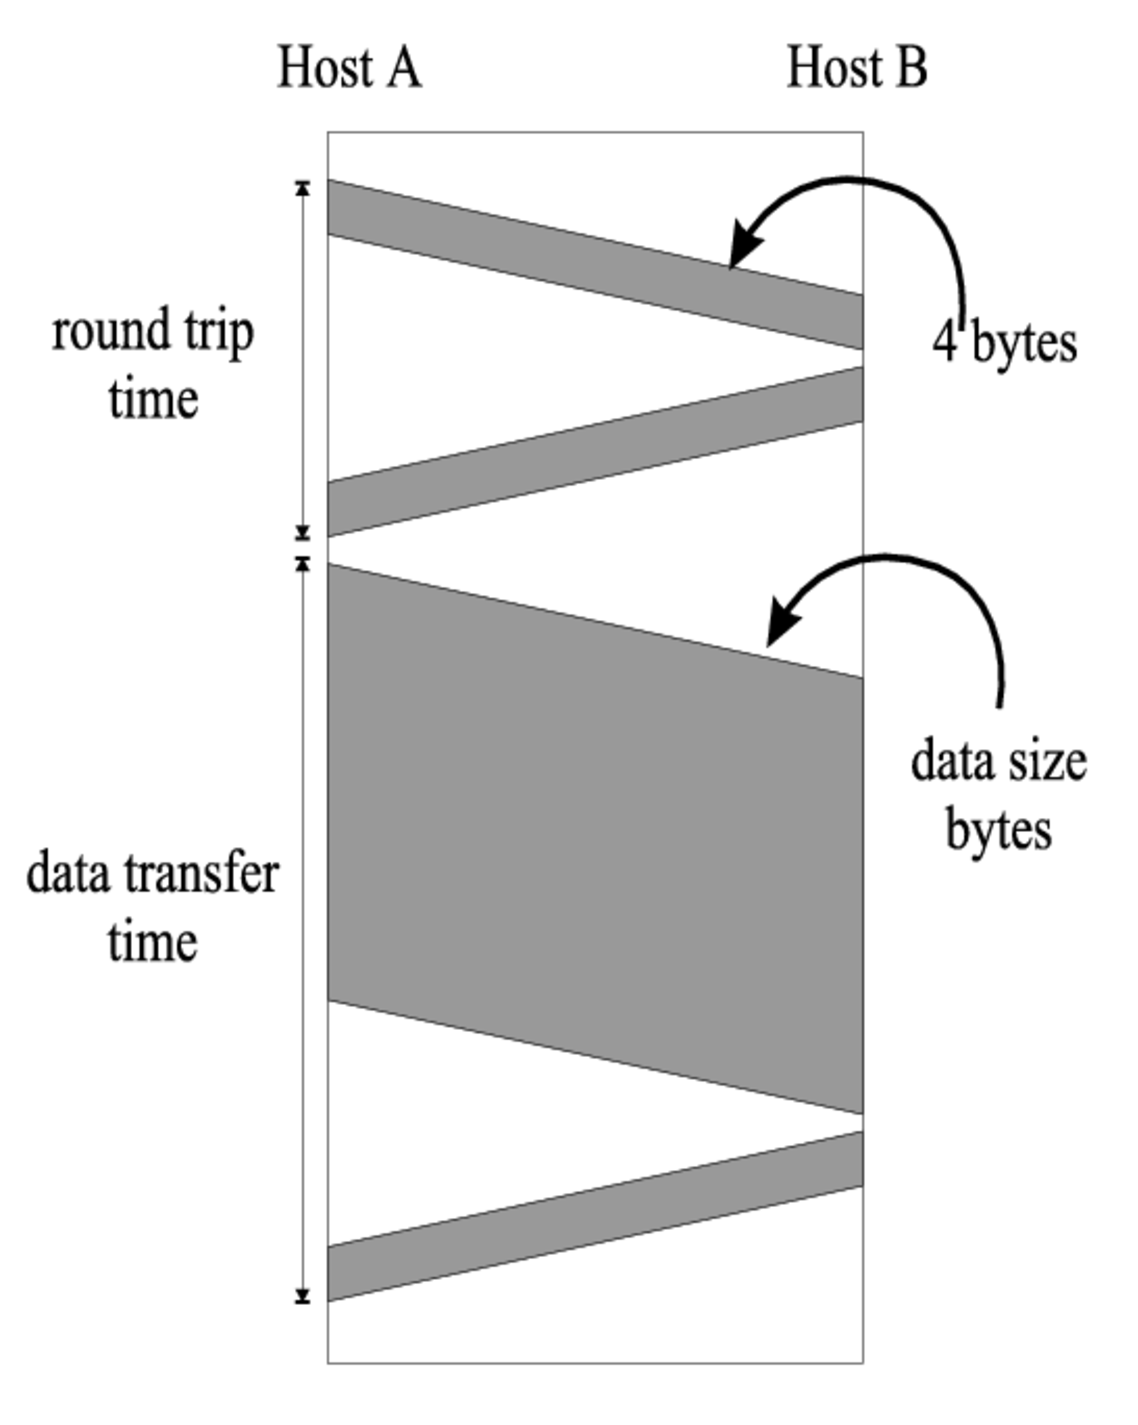
\includegraphics[width=0.5\linewidth]{images/topologie/NWS}
%			\par\end{centering}
%		
%		\caption{\label{fig:NWS}Procédure de NWS pour l'obtention de la latence et
%			du débit}
%		
%	\end{figure}
%	
%	
%	Le débit, par contre, est estimé en chronométrant le temps nécessaire
%	à l'envoi des paquets de plus grande taille (par exemple 64 Ko) et
%	en retirant le temps relatif à la latence de transmission des messages.
%	Le choix de la valeur des paquets de grande taille permet de mesurer
%	un réseau local classique tout en limitant l'intrusivité des expérimentations. 
%	
%	Il reste toutefois la contrainte que les mesures de NWS sont limitées
%	par l'utilisation d'un seul \emph{socket} sur une seule machine. En
%	effet, cette approche n'est pas adaptée aux réseaux de très haut débit. Par conséquence, NWS détecte une bande passante
%	maximale de l'ordre de 100 Mb/s sur VTHD, alors que ce réseau est capable d'atendre 2,5Gb/s \cite{Quinson03}, même en
%	réglant convenablement les paramètres des tests. Ceci indique clairement
%	que le capteurs NWS a atteint le maximum de bande passante qu'une application
%	utilisant un seul \emph{socket} réussit à occuper. 
%	
%	Il est aussi important de s'assurer qu'un même lien n'est jamais utilisé
%	par deux tests de bande passante concurrents au même instant. Dans
%	ce cas de collision entre deux mesures, les flux se partageraient
%	la bande passante disponible sur le lien, ce qui fausserait les résultats
%	(chaque test pourrait donner un résultat égal à la moitié de la valeur
%	réelle). Pour éviter ce problème, NWS introduit la notion de \textit{clique}
%	: tous les hôtes appartenant à une même \textit{clique} sont réputés partager
%	une ressource réseau, et NWS s'assure que les tests menés entre ces
%	liens n'entrent pas en collision. Un algorithme d'élection de leader
%	par passage de jeton est utilisé pour cela, et seul l'hôte en possession
%	du jeton à un instant donné est autorisé à initier un test réseau.
%	
%
%%
%%\subsubsection{Détection d'interférences}
%%
%%
%%\subsubsection*{TopoMon}
%%
%%Malgré la possibilité d'éviter la collision entre deux mesures par
%%l'utilisation des \textit{cliques}, NWS n'est pas capable d'assurer que les
%%différentes cliques ne partagent pas des liens en commun. La détection
%%de possibles interférences est alors une nécessité, d'autant plus
%%que le routage WAN n'est pas facilement connu.
%%
%%Dans le but d'identifier les liens partagés par différents noeuds,
%%et de cette manière automatiser le déploiement de NWS, l'outil TopoMon
%%\cite{Burger02} utilise \emph{traceroute}. Par évaluation des routes,
%%TopoMon détecte les machines groupées sous le même réseau, et peut
%%ainsi fournir à NWS des informations plus précises pour la disposition
%%des cliques.
%%
%%
%%\subsubsection*{ENV - Effective Network View}
%%
%%Le projet Effective Network View (ENV \cite{Shao99}) a pour principe
%%de mesurer directement les interférences entre les flux de données.
%%Pour cela, la bande passante normale entre deux machines données est
%%comparée à celle obtenue lorsqu'un autre lien (entre deux autres machines)
%%est saturé. Une variation indique que les deux liens partagent des
%%ressources réseau, et cette information est utilisée pour construire
%%la topologie d'interconnexion des machines. ENV utilise uniquement
%%des expérimentations de niveau applicatif, ne nécessitant donc pas
%%de privilèges ou d'outils spéciaux. En revanche, l'obtention de la
%%vue complète de la topologie requiert une grande quantité d'expériences.
%%En effet, il faut tester les éventuelles interactions du lien connectant
%%chaque paire de machines avec chaque autre lien, ce qui conduit à
%%un algorithme en $O(n^{4})$ pour \emph{n} machines. De plus, chaque
%%expérience requiert que le réseau soit stabilisé, ce que ne permettrait
%%de faire que quelques expériences par minute. L'approche choisie pour
%%ENV alors est de représenter le réseau seulement du point de vue d'une
%%machine donnée, approche suffisante pour les applications qui suivent
%%le paradigme maître/esclave.
%%
%%
%%\subsubsection*{ALNeM - Application-Level Network Mapper}
%%
%%L'une des restrictions de ENV est qu'il ne permet pas d'obtenir la
%%topologie complète de la plate-forme, mais seulement une vue arborescente
%%enracinée en un point arbitraire du réseau. Il est donc impossible
%%d'obtenir par ce biais des informations sur les liens connectant des
%%machines (autres que le maître choisi) entre elles. Malheureusement,
%%certaines solutions de cartographie du réseau présentées précédemment
%%ne sont pas adaptées à un contexte de \emph{metacomputing}. Le projet
%%ALNeM (Application-Level Network Mapper - outil de découverte de la
%%topologie de niveau applicatif) \cite{Legrand03,Quinson03,Legrand04}
%%vise à l'identification des constituants de la grille et leur distribution
%%logique, obtenue à partir de leurs interactions réseau.
%%
%%Afin d'accélérer le processus de découverte du réseau, ALNeM mène
%%les expériences en parallèle en tirant parti de l'existence de liens
%%indépendants. Puisqu'ils n'interfèrent pas les uns sur les autres,
%%il est possible de saturer plusieurs de ces liens en parallèle, et
%%une enquête plus approfondie est menée seulement si une baisse de
%%performance est détectée lors des expérimentations de multiples liens
%%en parallèle. Afin de prédire les liens probablement indépendants
%%et guider l'algorithme de découverte du réseau, une étape préliminaire
%%fait une approximation de la topologie grâce à \emph{traceroute}. 
%%
%
%
%\subsection{\label{cha: topo MPI}Découverte de la Topologie}
%
%Dans les sections précédentes nous avons étudié quelques outils pour
%la découverte de topologie. En ce qui concerne la découverte de topologie
%pour les applications distribuées, nous considérons que le découpage
%du réseau doit se faire préférentiellement par rapport à l'environnement
%de l'application car celui-ci peut influencer
%les temps de communication. Les outils de surveillance du réseau présentés
%précédemment, malgré leur importance, n'ont pas pour objectif l'obtention
%de paramètres de communication précis pour la modélisation des communications,
%et donc ne peuvent pas assurer la précision nécessaire à notre travail. 
%
%En effet, la plupart de ces outils acquièrent des informations à des
%niveaux assez proches de la couche matérielle, qui parfois ne reflète
%pas l'environnement de l'application. D'autres outils, sont plus intéressés aux interactions
%des liens de communication, qui malgré son importance, ont pour désavantage
%le coût excessif des mesures et une forte intrusivité sur le réseau.
%De surcroît, les informations de connectivité varient d'un outil à
%l'autre, alors que nous aimerions des informations de connectivité
%qui puissent être directement utilisées pour nos modèles de performance. 
%
%Une autre préoccupation de notre travail est de limiter l'intrusivité
%des procédures de découverte de topologie. En effet, même si quelques
%outils ont déjà des stratégies pour limiter le nombre de messages
%échangés et la perturbation sur le réseau, la propriété de \textbf{l'Exhaustivité}
%exigée par notre travail et présentée en page \pageref{sub:Topologie-recherch=0000E9e}
%n'est pas toujours respectée.
%
%Dans ce travail, nous proposons une alternative mixte, adaptée à nos
%exigences pour la modélisation des performances de communication,
%mais avec une forte conscience sur la perturbation du réseau et la
%scalabilité des systèmes. Cette proposition, structurée comme un \emph{framework}
%\cite{Steffenel04b} dédié à la découverte automatique de la topologie
%du réseau, est utilisée dans l'objectif d'optimiser la modélisation
%des communications collectives et permettre la construction de primitives
%adaptées à l'environnement hétérogène des grilles de calcul. 
%
%Ainsi, nous proposons une approche mixte pour la découverte de topologie,
%qui se déroule en trois étapes : la première étape est responsable
%de la collecte des informations de connectivité des différents réseaux
%et de façon indépendante ; la deuxième étape, plus proche de l'application,
%sert à identifier la distribution des processus sur les machines,
%découper les réseaux en îlots de communication homogène (grappes logiques). 
%Finalement, une troisième étape nous permet d'obtenir les paramètres pLogP nécessaires aux modèles
%de communication. 
%
%Comme la première partie est indépendante de l'application, elle peut
%utiliser des informations fournies par d'autres outils de surveillance
%du réseau (par exemple, NWS \cite{Wolski97}) voir des informations
%fournies pour l'utilisateur ou le service de réservation des noeuds. Ces informations
%sont utilisées pour construire une matrice de distance qui servira
%de base à notre découverte de topologie. Pour une question de simplicité,
%nous considérons que cette matrice de distances est creuse, dans le
%sens que une grappe n'est pas obligée à surveiller ses interconnexions
%avec les autres grappes. Cette matrice peut contenir des différents
%paramètres de connectivité qui seront utilisés pour classifier les
%noeuds et les liens, notamment la latence et le débit.
%
%La matrice de distance obtenue dans la première partie est communiquée
%à l'application, son framework d'exécution ou bien à l'environnement de déploiement. Les processus sont alors organisés en sous-réseaux homogènes, et les paramètres d'interconnexion entre ceux sous-réseaux sont acquis. Parce que le
%réseau est structuré en sous-réseaux homogènes, l'obtention des paramètres
%se fait d'une manière optimisée, réduisant ainsi l'impact des mesures
%sur la performance du réseau et l'initialisation de l'application.
%
%De cette manière, à la fin du processus de découverte de topologie
%nous avons des grappes logiques composées de machines homogènes, et
%des paramètres d'interconnexion suffisamment précis pour permettre
%la construction des arbres d'interconnection qui optimisent à la fois
%les communications collectives à l'intérieur et à l'extérieur des
%grappes.
%
%
%\subsection{\label{sec:First-Phase:-Gathering}Première partie : collecte des
%informations topologiques}
%
%La plupart des travaux sur l'optimisation des communications collectives
%pour les environnements de grille considèrent, par simplicité, que
%les grappes sont définies par sa localisation physique ou le sous-réseau
%IP, et que toutes les machines à l'intérieur d'une grappe sont similaires.
%Or, cette hypothèse de localité n'est pas totalement adaptée aux systèmes
%réels, qui peuvent contenir des machines avec différentes performances
%de calcul et de communication. En effet, même les grappes avec des
%machines identiques présentent des performances différentes (nous
%croyons qu'il est pratiquement impossible d'avoir l'homogénéité de
%ressources dans une grappe avec quelques centaines de machines). Par
%conséquent, le choix de la topologie du réseau doit préférablement
%se faire par des aspects opérationnels, qui reflètent la performance
%réelle des machines et des liens.
%
%Comme expliqué dans le chapitre précédent, l'acquisition des informations
%de connectivité peut se faire à travers des outils de surveillance
%du réseau. Par simplicité, nous considérons que ces informations sont obtenues
%au niveau de l'utilisateur, avec des tests similaires à ceux de NWS.
%Nous avons choisi NWS par le fait qu'il est l'outil \emph{de facto}
%de la communauté grille, et qu'il peut fournir des diverses informations
%comme la latence, le débit, l'utilisation des CPUs et la mémoire disponible
%sur les machines. Nous sommes particulièrement intéressés pour les
%informations de latence et débit, plus utiles pour identifier les
%groupes de machines avec de paramètres de communication similaires. 
%
%L'objectif de cette première partie est de découvrir les hétérogénéités cachées
%à l'intérieur des grappes, et pour cela, chaque grappe peut utiliser
%son propre système de surveillance, sans avoir besoin de contacter
%les autres grappes. Ainsi, cette stratégie permet la réduction du
%nombre de messages échangés sur le réseau, mais aussi permet l'utilisation
%des informations des services de surveillance, généralement plus corrects
%que des observations ponctuelles. 
%
%Les données de connectivité des différentes grappes sont réunies dans
%une unique matrice de distance. Comme les grappes ne sont pas conscientes
%des autres grappes, les interconnexions "manquantes" clairement
%délimitent les frontières de chaque grappe, réduisant ainsi le coût
%du processus de partitionnement qui sera effectué dans la deuxième
%partie de notre découverte de topologie. 
%
%
%\subsection{\label{sec:Second-Phase:-Network}Deuxième partie : partitionnement}
%
%À partir des données d'interconnexion obtenues dans la partie précédente,
%notre objectif initial est de regrouper les noeuds en grappes logiques
%différentes. Pour cela, des algorithmes de partitionnement (\emph{clustering})
%se font nécessaires. 
%
%Le partitionnement des noeuds peut se faire à travers l'organisation
%hiérarchique des noeuds, ou alors à travers le simple découpage en
%groupes isolés (bulles). Un exemple de la première approche est présenté
%par \cite{Jain91}, et le résultat est une arborescence où les noeuds
%proches sont regroupés sous les mêmes branches de l'arbre. Le désavantage
%de cette méthode est qu'elle présente une structure figée, qui n'est
%pas nécessairement adaptée à l'ensemble de communications collectives
%existantes.
%
%L'autre approche, au contraire, se limite à regrouper les noeuds qui
%ont une différence $\rho$ préalablement définie. Pour cela, on considère
%un graphe $G=(V,E)$, composé de $V=\{1,2,\ldots,|V|\}$ noeuds et
%des arcs $\{i,j\}$, chacun avec un poids $E_{j,i}$. La matrice de
%distances \emph{M} est définie comme\[
%M=\left\{ \begin{array}{c}
%\begin{array}{cc}
%E_{i,j} & \:\:\:\:\:\:\:\:\:\:\:\:\:\:\:\:\:\:\:\:\: si\: existe\: un\: lien\: local\: entre\:\{i,j\}\\
%0 & dans\: le\: cas\: contraire\end{array}\end{array}\right.\]
%
%
%Par exemple, si on considère que \emph{$E(x,y)$} est la latence entre
%deux noeuds \emph{x} et \emph{y}, et $\rho$ est la différence maximale
%entre deux noeuds qui font partie du même groupe, l'algorithme le
%plus général pour cette approche considère que :
%
%\[
%\forall x,\forall y\in S,x\neq y,\; a\in S\Rightarrow\left|E(a,x)-E(x,y)\right|\leq\rho\]
%
%
%Le problème de cette approche est que pour chaque nouveau noeud, il
%faut comparer sa distance avec tous les autres noeuds qui sont à l'intérieur
%d'un groupe.
%
%Une approche moins complexe est présentée par Lowekamp \cite{Lowekamp00}
%et utilisée dans la bibliothèque ECO (Algorithme \ref{cap:ECO-algorithm-for}).
%En effet, ECO utilise un algorithme glouton qui considère que :
%
%\[
%\forall x,\forall y\in S,x\neq y,\; a\in S\Rightarrow\left|E(a,x)-min(E(x,y))\right|\leq\rho\]
%
%
%%
%\begin{algorithm}[h]
%\caption{\label{cap:ECO-algorithm-for}Algorithme de Lowekamp \cite{Lowekamp00}
%pour le partitionnement du réseau ($\rho=20$\%)}
%
%
%\texttt{\scriptsize initialize subnets to empty}{\scriptsize \par}
%
%\texttt{\scriptsize for all nodes}{\scriptsize \par}
%
%\texttt{\scriptsize ~~node.min\_edge = minimum cost edge incident
%on node}{\scriptsize \par}
%
%\texttt{\scriptsize sort edges by nondecreasing cost}{\scriptsize \par}
%
%\texttt{\scriptsize for all edges (a,b)}{\scriptsize \par}
%
%\texttt{\scriptsize ~~if a and b are in the same subnet}{\scriptsize \par}
%
%\texttt{\scriptsize ~~~~continue}{\scriptsize \par}
%
%\texttt{\scriptsize ~~if edge.weight>1.20 {*} node(a).min\_edge
%or edge.weight>1.20 {*} node(b).min\_edge}{\scriptsize \par}
%
%\texttt{\scriptsize ~~~~continue}{\scriptsize \par}
%
%\texttt{\scriptsize ~~if node (a) in a subnet}{\scriptsize \par}
%
%\texttt{\scriptsize ~~~~if (edge.weight>1.20 {*} node(a).subnet\_min\_edge)}{\scriptsize \par}
%
%\texttt{\scriptsize ~~~~~~continue}{\scriptsize \par}
%
%\texttt{\scriptsize ~~if node (b) in a subnet}{\scriptsize \par}
%
%\texttt{\scriptsize ~~~~if (edge.weight>1.20 {*} node(b).subnet\_min\_edge)}{\scriptsize \par}
%
%\texttt{\scriptsize ~~~~~~continue}{\scriptsize \par}
%
%\texttt{\scriptsize ~~merge node(a).subnet and node(b).subnet}{\scriptsize \par}
%
%\texttt{\scriptsize ~~set subnet\_min\_edge to min(edge,node(a).subnet\_min\_edge,
%node(b).subnet\_min\_edge)}
%\end{algorithm}
%
%
%Dans cette approche, chaque sous-réseau garde la valeur du plus petit
%arc à l'intérieur du groupe. Chaque nouvel arc est comparé avec cette
%valeur minimum, réduisant ainsi le nombre de comparaison à effectuer.
%
%La contrepartie de l'algorithme de Lowekamp est qu'il permet certaines
%situations où des sous-réseaux hétérogènes sont formés. La Figure
%\ref{Fig:ECOwrong} présente un exemple de ce problème, où des noeuds
%hétérogènes sont incorrectement regroupés. 
%
%%
%\begin{figure}[h]
%\begin{centering}
%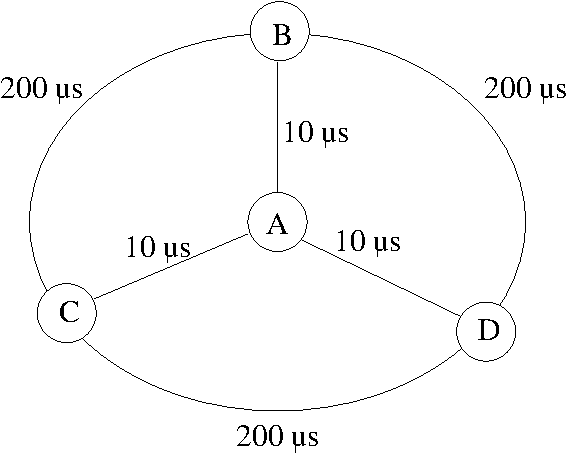
\includegraphics[scale=0.5]{images/topologie/Lowkamp-mistake}
%\par\end{centering}
%
%\caption{\label{Fig:ECOwrong}Contre-exemple à l'algorithme de Lowekamp}
%
%\end{figure}
%
%
%En effet, nous pouvons observer que le noeud A est le seul connecté
%aux autres avec une petite latence. Or, dans ce cas, un groupe \{A,
%B, C, D\} est possible, malgré le fait que l'interconnexion entre
%les noeuds B, C et D est beaucoup plus lente. Dans ce cas, l'hétérogénéité
%des connexions à l'intérieur du groupe peut influencer fortement les
%communications (par exemple, si B devient le coordinateur), sans que
%les modèles de communication soient capables de représenter les performances
%obtenues. Cependant, telles situations sont suffisamment rares pour
%permettre l'utilisation de l'algorithme de Lowekamp dans notre outil
%de découverte de topologie. 
%
%
%\subsection{\label{sec:Getting-pLogP-data}Troisième partie : acquisition efficace
%des paramètres d'interconnexion}
%
%Même si les grappes logiques identifiées par notre \emph{framework}
%présentent la structure effective du réseau, nous ne sommes pas encore
%en mesure de modéliser les communications avec précision. La première
%raison est que la matrice de distances n'est pas totalement remplie.
%Comme expliqué dans la section \ref{sec:First-Phase:-Gathering},
%l'obtention des informations de connectivité se fait localement à
%chaque grappe, et les connexions entre les grappes ne sont pas encore
%établies. 
%
%Une autre raison est que les données obtenues par les outils de surveillance
%du réseau ne sont pas adaptées à nos modèles de communication. Par
%exemple, la latence est obtenue de façon différente par les outils
%NWS \cite{Wolski97} et LogP-MPI \cite{Kielmann00}. Dans le cas de
%NWS, la latence est obtenue directement à partir du temps d'aller-retour
%d'un message. L'outil LogP-MPI, par contre, décompose le temps d'aller-retour
%en deux composants, la latence et le \emph{gap}, comme illustré dans
%la Figure \ref{Figure:Differences-between-NWS}. Les différences entre
%les deux stratégies d'obtention de la latence sont suffisamment grandes
%pour interférer sur la précision des modèles de communication. 
%
%%
%\begin{figure}[h]
%\begin{centering}
%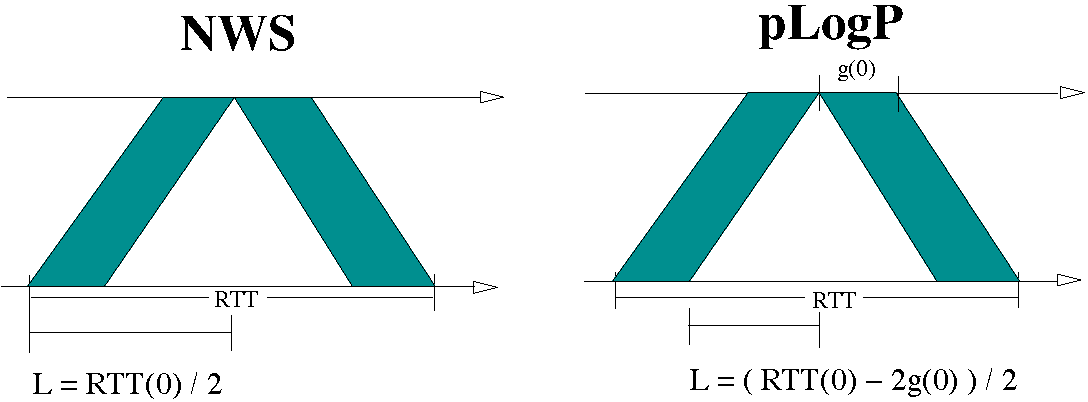
\includegraphics[width=0.9\linewidth,keepaspectratio]{images/topologie/NWSxpLogP}
%\par\end{centering}
%
%\caption{\label{Figure:Differences-between-NWS}Différence entre la latence
%de NWS et de pLogP}
%
%\end{figure}
%
%
%Heureusement, nous n'avons plus besoin d'exécuter $n(n-1)$ mesures,
%une pour chaque interconnexion possible. En effet, l'homogénéité des
%grappes logiques permet qu'une seule mesure des paramètres d'interconnexion
%à l'intérieur de chaque grappe soit suffisante pour représenter toutes
%les communications à l'intérieur cette grappe. De même, il suffirait
%de mesurer une connexion entre chaque grappe pour représenter toutes
%les connexions distantes possibles. 
%
%Finalement, nous pouvons encore réduire le nombre de mesures par moitié,
%si nous considérons que les liens de connexion sont symétriques $a\rightarrow b=b\rightarrow a$.
%Ainsi, se le nombre de grappes logiques identifiées précédemment est
%C, la quantité de mesures est réduite à :
%
%\[
%\frac{C\times(C-1)}{2}+C\]
%
%
%\subsubsection*{Obtention des paramètres}
%
%Comme pLogP est le modèle le plus souple pour représenter les différents algorithmes
%de communication collective, il est aussi important
%de bien obtenir les paramètres nécessaires à ce modèle.
%
%Pour cela, nous avons utilisé la méthode proposée et implantée par
%Kielmann \cite{Kielmann00}. L'avantage de cette méthode par rapport
%à des techniques précédentes comme celles de Culler \cite{Culler96b}
%et Ianello \cite{Ianello97} réside dans l'obtention du paramètre
%\emph{gap}. En effet, les méthodes décrits par Culler et Ianello utilisent
%des grands messages pour saturer le réseau, afin que le débit du lien
%(représenté par le \emph{gap}) soit mesuré. Cependant, cette technique
%est très intrusive et nécessite un temps assez élevé pour mesurer
%le gap dans les réseaux à très haut débit.
%
%Dans l'approche proposé par Kielmann, par contre, le gap est obtenu
%à partir de l'envoi de petits messages de taille zéro. Ainsi, pour
%mesurer \emph{g(0)}, la méthode proposé mesure le temps d'aller-retour
%d'un message de taille zéro - $RTT_{1}(0)$ - entre deux processus,
%\emph{measure} et \emph{mirror}. Ensuite, le nombre de messages envoyés
%simultanés est augmenté, de manière à ce que le temps $RTT_{n}(0)$
%indique le temps nécessaire à l'envoi de \emph{n} messages vers le
%\emph{mirror} suivies d'une unique réponse d'acquittement vers le
%\emph{measure}. Le nombre de messages \emph{n} est doublé jusqu'à
%ce que le \emph{gap} par message ne varie que de d'une marge d'erreur
%$\epsilon$. À ce point, $RTT_{n}(0)$ est considéré comme équivalent
%à \emph{$n\times g(0)$} et la valeur de \emph{$g(0)$} peut être
%facilement obtenue. 
%
%En effet, un premier échange envoie un message de \emph{m} octets,
%qui est répondu par un message de taille zéro (c'est équivalent à
%faire $RTT_{1}(m)$). À partir de $RTT_{1}(m)$, les valeurs de $g(m)$
%et \emph{L} peuvent être déduites directement à partir des équations
%présentées dans le Tableau \ref{Tableau:pLogp_Equations}.
%
%%
%\begin{table}[h]
%	\caption{\label{Tableau:pLogp_Equations}Équations pour l'obtention de $g(m)$
%		avec pLogP \cite{Kielmann00}}
%	
%	
%	\begin{centering}
%		\begin{tabular}{|c|}
%			\hline 
%			$RTT_{1}(0)=2\times(L+g(0))$\tabularnewline
%			$L=(RTT_{1}(0)-2\times g(0))/2$\tabularnewline
%			$RTT_{1}(m)=L+g(m)+L+g(0)$\tabularnewline
%			$g(m)=RTT_{1}(m)-RTT_{1}(0)+g(0)$\tabularnewline
%			\hline
%		\end{tabular}
%		\par\end{centering}
%\end{table}
%
%
%Pour obtenir les autres paramètres comme $o_{s}(m)$ et $o_{r}(m)$,
%nous utilisons la procédure représentée dans la Figure \ref{Figure: pLogP_acquisition}.
%Dans un premier moment, le paramètre $o_{s}(m)$ est obtenu à partir
%de la mesure du temps de l'envoi simple (sans attendre une réponse).
%Dans le deuxième échange de messages, le processus \emph{measure}
%envoie un message de taille zéro et attend pendant un temps $\Delta>RTT_{1}(m)$
%avant de recevoir un message de \emph{m} octets. Cet échange permet
%l'obtention de $o_{r}(m)$, car après le temps $\Delta>RTT_{1}(m)$
%le processus \emph{measure} est certain que le message envoyé par
%\emph{mirror} est déjà disponible dans la mémoire tampon de son interface
%réseau. Il faut observer cependant que cette mesure de $o_{r}(m)$
%n'est correcte que si la communication entre les deux noeuds \emph{measure}
%et \emph{mirror} est symétrique. Si le débit entre \emph{mirror} et
%\emph{measure} est moins important que celui entre \emph{measure}
%et \emph{mirror}, cela peut donner des valeurs de $o_{r}(m)$ plus
%grands que $g(m)$. Ainsi, une manière d'éviter cette situation serait
%de mesurer $o_{r}(m)$ dans une communication \emph{measure-measure},
%si $o_{r}(m)$ est un paramètre essentiel aux modèles étudiés.
%
%%
%\begin{figure}[h]
%	\begin{centering}
%		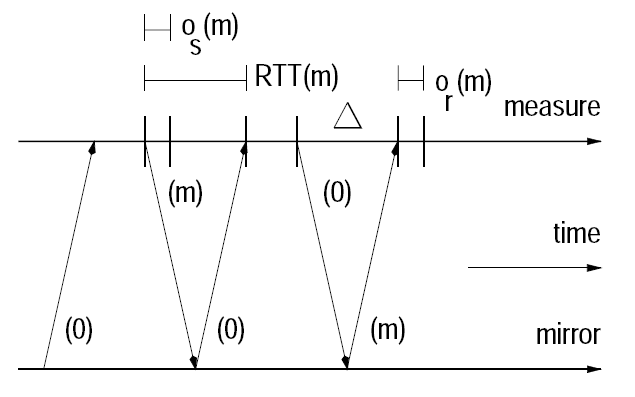
\includegraphics[width=0.55\linewidth]{images/p2p/pLogP_acquiring}
%		\par\end{centering}
%	
%	\caption{\label{Figure: pLogP_acquisition}Méthode d'obtention des paramètres
%		pLogP \cite{Kielmann00}}
%	
%\end{figure}
%
%
%Répété avec différentes valeurs de \emph{m}, cette procédure permet
%l'obtention de $g(m)$, $o_{s}(m)$ et $o_{r}(m)$ à partir d'un tableau
%contenant une liste d'échantillons, comme présenté dans la Figure
%\ref{Figure:exemple fichier pLogP}. Ces échantillons sont obtenus
%de manière à ce que la détermination des valeurs pour une taille de
%message \emph{m} donnée soit faite à partir de l'interpolation des
%points de mesure les plus proches.
%
%%
%\begin{figure}[h]
%	\begin{centering}
%		{\footnotesize }\begin{tabular}{|l|}
%			\hline 
%			{\footnotesize \texttt{}\foreignlanguage{english}{{\footnotesize \#
%						LogP network performance data: logp\_test-Send-Recv}}{\footnotesize }}\tabularnewline
%			{\footnotesize \texttt{}\foreignlanguage{english}{{\footnotesize \#
%						Latency = 32.66}}{\footnotesize }}\tabularnewline
%			{\footnotesize \texttt{}\foreignlanguage{english}{{\footnotesize \#
%						time }\textbf{\footnotesize bytes}{\footnotesize{} os os\_min os\_cnfint
%						or or\_min or\_cnfint }\textbf{\footnotesize g}}{\footnotesize }}\tabularnewline
%			{\footnotesize \texttt{}\foreignlanguage{english}{{\footnotesize 1113829432
%					}\textbf{\footnotesize 0}{\footnotesize{} 0.0000053 0.0000043 0.0000004
%					0.0000024 0.0000014 0.0000009 }\textbf{\footnotesize 0.0000014}}{\footnotesize }}\tabularnewline
%		{\footnotesize \texttt{}\foreignlanguage{english}{{\footnotesize 1113829432
%				}\textbf{\footnotesize 1}{\footnotesize{} 0.0000056 0.0000043 0.0000005
%				0.0000036 0.0000024 0.0000004 }\textbf{\footnotesize 0.0000035}}{\footnotesize }}\tabularnewline
%	{\footnotesize \texttt{}\foreignlanguage{english}{{\footnotesize 1113829432
%			}\textbf{\footnotesize 2}{\footnotesize{} 0.0000058 0.0000043 0.0000004
%			0.0000038 0.0000033 0.0000010 }\textbf{\footnotesize 0.0000036}}{\footnotesize }}\tabularnewline
%{\footnotesize \texttt{...}}\tabularnewline
%{\footnotesize \texttt{}\foreignlanguage{english}{{\footnotesize 1113829432
%		}\textbf{\footnotesize 256}{\footnotesize{} 0.0000059 0.0000043 0.0000005
%		0.0000042 0.0000033 0.0000007 }\textbf{\footnotesize 0.0000090}}{\footnotesize }}\tabularnewline
%{\footnotesize \texttt{}\foreignlanguage{english}{{\footnotesize 1113829432
%		}\textbf{\footnotesize 512}{\footnotesize{} 0.0000061 0.0000045 0.0000011
%		0.0000041 0.0000033 0.0000009 }\textbf{\footnotesize 0.0000158}}{\footnotesize }}\tabularnewline
%{\footnotesize \texttt{}\foreignlanguage{english}{{\footnotesize 1113829432
%		}\textbf{\footnotesize 1024}{\footnotesize{} 0.0000063 0.0000052 0.0000010
%		0.0000044 0.0000033 0.0000004 }\textbf{\footnotesize 0.0000292}}{\footnotesize }}\tabularnewline
%{\footnotesize \texttt{...}}\tabularnewline
%{\footnotesize \texttt{}\foreignlanguage{english}{{\footnotesize 1113829432
%		}\textbf{\footnotesize 262144}{\footnotesize{} 0.0017727 0.0017314
%		0.0001001 0.0023521 0.0023274 0.0001276 }\textbf{\footnotesize 0.0023500}}{\footnotesize }}\tabularnewline
%{\footnotesize \texttt{}\foreignlanguage{english}{{\footnotesize 1113829433
%		}\textbf{\footnotesize 524288}{\footnotesize{} 0.0039728 0.0038664
%		0.0002125 0.0046024 0.0045595 0.0002578 }\textbf{\footnotesize 0.0045943}}{\footnotesize }}\tabularnewline
%{\footnotesize \texttt{}\foreignlanguage{english}{{\footnotesize 1113829433
%		}\textbf{\footnotesize 1048576}{\footnotesize{} 0.0085095 0.0084665
%		0.0002588 0.0090407 0.0090144 0.0001601 }\textbf{\footnotesize 0.0091020}}{\footnotesize }}\tabularnewline
%{\footnotesize \texttt{...}}\tabularnewline
%\hline
%\end{tabular}{\footnotesize{} }
%\par\end{centering}{\footnotesize \par}
%
%\caption{\label{Figure:exemple fichier pLogP}Exemple d'un tableau avec les
%	paramètres pLogP pour des tailles de message différentes (1 octet
%	jusqu'à 1Mo)}
%
%\end{figure}
%
%
%
%\subsection{\label{sec:Practical Results}Évaluation pratique}
%
%Pour évaluer l'utilisation de notre \emph{framework}, nous avons intégré
%les trois parties de découverte de topologie dans la bibliothèque
%LaPIe, une bibliothèque MPI conçue pour optimiser pour les communications collectives (broadcast, gather, scatter, all-to-all, etc.) dans les environnments de type grille hétérogène. Les deux premières parties du framework sont implantées en une application
%indépendante, alors que la troisième partie est implantée directement dans les
%procédures d'initialisation du MPI.
%
%\subsubsection{Clusterisation}
%
%En effet, les étapes de collecte d'informations et de partitionnement
%des machines ont été regroupées en une application indépendante, exécutée
%par l'utilisateur avant le déploiement de son application, et qui
%fournit un fichier de description des grappes homogènes. Nous avons
%profité des fonctionnalités de la bibliothèque MagPIe, dont nous sommes
%inspirés, pour fournir à l'application une description de la répartition
%des machines qui sera utilisée ensuite pour la construction de la
%topologie des processus. Seule différence, notre bibliothèque a permis
%l'automatisation de la génération de ce fichier de description, ce
%qui est notamment avantageux du point de vue des heuristiques d'optimisation
%qui utilisent cette description.
%
%La troisième partie a été intégrée à la fonction \emph{MPI\_Init},
%appelée à l'initialisation de chaque application MPI. Nous avons intégré
%les fonctions d'obtention des paramètres d'interconnexion aux fonctions
%de description de la topologie. Cela permet notamment la prise en
%charge des coûts de communication réels de l'application.
%
%Pour illustrer notre approche de découverte de topologie, notamment
%la première et la deuxième partie, nous présentons deux expériences,
%l'une sur la grappe IDPOT à Grenoble, et l'autre sur une grille de 78 machines
%réparties entre les sites d'Orsay, Toulouse, Sophia-Antipolis et Grenoble
%(IDPOT). 
%
%La grappe IDPOT était constituée de machines Intel Xeon biprocesseur
%dont une partie des machines utilise des cartes réseau Broadcom Giga
%Ethernet et l'autre partie utilise des cartes réseau Intel Giga Ethernet.
%L'interaction entre les différentes cartes réseau occasionne une forte
%variation de performance des communications, ce qui est très intéressante
%pour les expériences de découverte du réseau (conformément à ce que
%nous avons présenté en \cite{Steffenel04b}). 
%
%À partir de la procédure de découverte de topologie présentée précédemment,
%nous avons pu repartir les machines IDPOT en trois groupes homogènes,
%comme indique la Figure \ref{Figure:exemplefichermagpie_idpot}.
%
%%
%\begin{figure}[h]
%\begin{centering}
%{\footnotesize }\begin{tabular}{|l|}
%\hline 
%{\footnotesize \texttt{cluster 0 }}\tabularnewline
%{\footnotesize \texttt{process 0 1 2 3 6 7 8 9 11 12 17}}\tabularnewline
%{\footnotesize \texttt{cluster 1 }}\tabularnewline
%{\footnotesize \texttt{process 4 5}}\tabularnewline
%{\footnotesize \texttt{cluster 2 }}\tabularnewline
%{\footnotesize \texttt{process 10 13 14 15 16}}\tabularnewline
%{\footnotesize \texttt{\# Min edge 0-0 = 35.524368}}\tabularnewline
%{\footnotesize \texttt{\# Min edge 0-1 = 59.962273}}\tabularnewline
%{\footnotesize \texttt{\# Min edge 0-2 = 59.962273}}\tabularnewline
%{\footnotesize \texttt{\# Min edge 1-1 = 60.439110 }}\tabularnewline
%{\footnotesize \texttt{\# Min edge 1-2 = 122.54715 }}\tabularnewline
%{\footnotesize \texttt{\# Min edge 2-2 = 60.081482 }}\tabularnewline
%\hline
%\end{tabular}{\footnotesize{} }
%\par\end{centering}{\footnotesize \par}
%
%\caption{\label{Figure:exemplefichermagpie_idpot}Fichier de description de
%grappes logique homogènes pour le réseau IDPOT, avec la latence entre
%les grappes (microsecondes)}
%
%\end{figure}
%
%
%Cette différence entre les machines IDPOT se reflète aussi sur le
%gap, comme indiqué dans le Tableau \ref{Tableau :Gap-IDPOT}, malgré
%le fait que les machines appartiennent toutes au même sous-réseau
%IP, technique normalement utilisée pour regrouper les machines. 
%
%En effet, une telle variation des valeurs des paramètres d'interconnexion
%(le gap et la latence) ne permet pas une prédiction de performance
%très précise, car les modèles de performance considèrent que le réseau
%est uniforme, c'est-à-dire, une valeur unique de gap et latence pour
%tout le réseau. À l'aide de notre outil pour la découverte de topologie
%nous pouvons alors identifier les sous-réseaux homogènes et les traiter
%séparément, de manière, par exemple, à réorganiser les communications
%selon les heuristiques présentées dans le chapitre \ref{cha:Comm sur grille}.
%En conséquence, l'identification des sous-réseaux homogènes rend possible
%une meilleure modélisation du réseau réel que le simple regroupement
%des noeuds par localisation ou sous-réseau IP.
%
%%
%\begin{table}
%\caption{\label{Tableau :Gap-IDPOT}Gap pour un message de 1Mo sur les sous-réseaux
%IDPOT, en millisecondes}
%
%
%\begin{centering}
%\begin{tabular}{|c||c|c|c|}
%\hline 
% & sous-réseau 0 & sous-réseau 1 & sous-réseau 2\tabularnewline
%\hline
%\hline 
%sous-réseau 0 & 9,0906 & 19,7898 & 16,4515\tabularnewline
%\hline 
%sous-réseau 1 & 19,7898 & 25,0942 & 25,2701\tabularnewline
%\hline 
%sous-réseau 2 & 16,4515 & 25,2701 & 26,1203\tabularnewline
%\hline
%\end{tabular}
%\par\end{centering}
%\end{table}
%
%
%La deuxième expérience réalisée considère une grille de 78 machines,
%dont 20 machines de la grappe GdX d'Orsay, 20 machines de la grappe
%de Toulouse, 19 machines de la grappe de Sophia-Antipolis et 17 machines
%de la grappe IDPOT.
%
%À l'aide de notre application de découverte de topologie (appelée
%\emph{subnets}), nous pouvons obtenir un fichier de description de
%la topologie similaire à celui présenté dans la Figure \ref{Figure:exemplefichermagpie_clusters}.
%
%%
%\begin{figure}[h]
%\begin{centering}
%{\footnotesize }\begin{tabular}{|l|}
%\hline 
%{\footnotesize \texttt{cluster 0 }}\tabularnewline
%{\footnotesize \texttt{process 0 1 2 3 4 5 6 7 8 9 10 11 12 13 14
%15 16 17 18 19 }}\tabularnewline
%{\footnotesize \texttt{cluster 1 }}\tabularnewline
%{\footnotesize \texttt{process 20 21 22 23 26 28 29 30 32 33 38 }}\tabularnewline
%{\footnotesize \texttt{cluster 2 }}\tabularnewline
%{\footnotesize \texttt{process 24 25 27 31 34 35 37 }}\tabularnewline
%{\footnotesize \texttt{cluster 3 }}\tabularnewline
%{\footnotesize \texttt{process 36 }}\tabularnewline
%{\footnotesize \texttt{cluster 4 }}\tabularnewline
%{\footnotesize \texttt{process 39 40 41 42 43 44 45 46 47 48 49 50
%51 52 53 54 55 56 57 58 }}\tabularnewline
%{\footnotesize \texttt{cluster 5}}\tabularnewline
%{\footnotesize \texttt{process 59 60 61 62 63 64 65 66 67 68 69 70
%71 72 73 74 75 76 77 }}\tabularnewline
%\hline
%\end{tabular}{\footnotesize{} }
%\par\end{centering}{\footnotesize \par}
%
%\caption{\label{Figure:exemplefichermagpie_clusters}Fichier de description
%de grappes logique homogènes}
%
%\end{figure}
%
%
%Il faut noter que les machines sont identifiées par le rang du processus
%MPI ; pour mieux identifier l'appartenance de chaque machine, nous
%présentons dans la Figure \ref{Figure: Topo Grille 78 machines} la
%distribution des six grappes homogènes par rapport à la localisation
%de ces machines.
%
%%
%\begin{figure}[h]
%\begin{centering}
%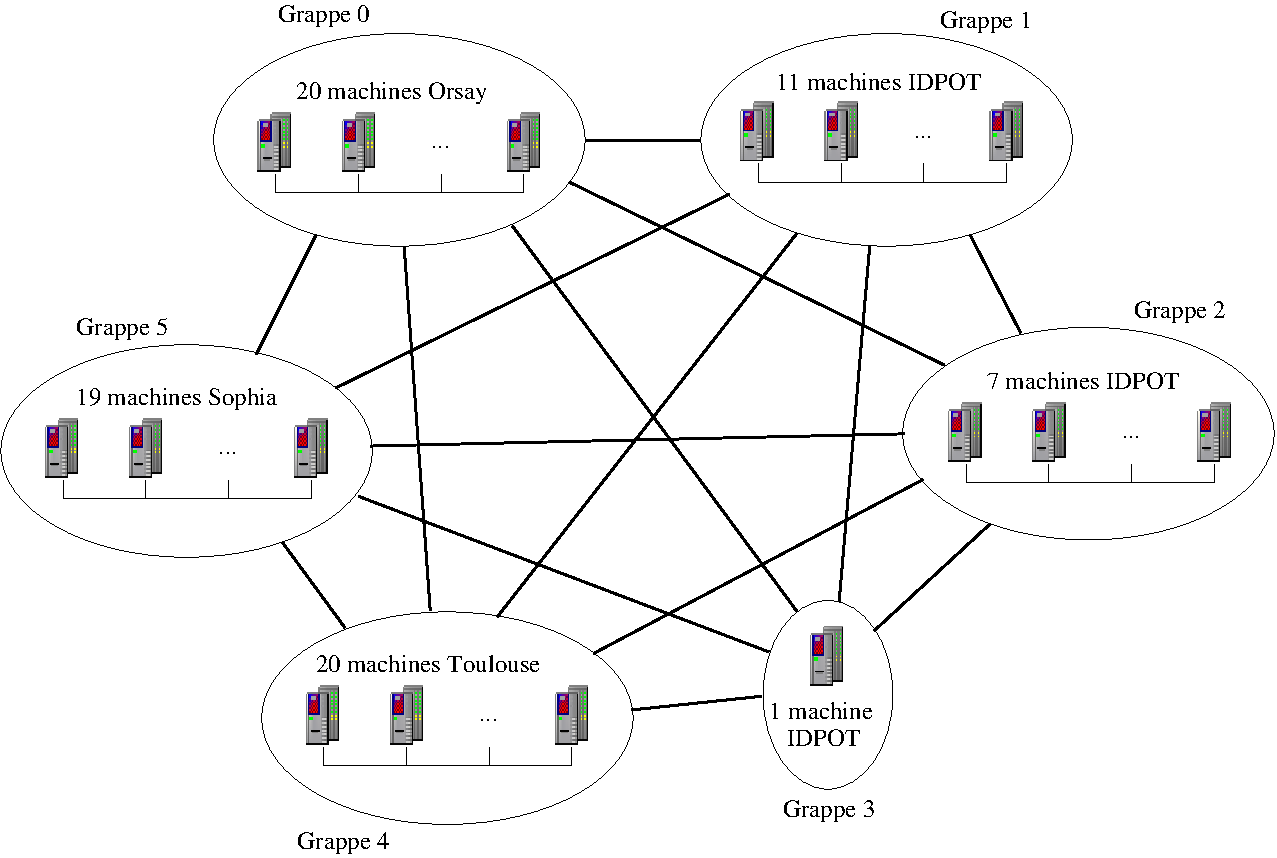
\includegraphics[width=0.75\linewidth]{images/Grid/Bcast/case2/grappe-case2}
%\par\end{centering}
%
%\caption{\label{Figure: Topo Grille 78 machines}Répartition des grappes homogènes
%dans une grille de 78 machines }
%
%\end{figure}
%
%
%Dans cet environnement, l'hétérogénéité est majoritairement due au
%facteur géographique. Cependant, le facteur matériel est aussi important,
%comme illustré par les machines du réseau IDPOT. Dans ce cas, nous
%observons que certaines machines peuvent être regroupées en grappes
%différentes malgré leur proximité géographique. Ainsi, les latences
%d'interconnexion entre les différents sites sont présentées dans le
%Tableau \ref{Tableau: topo case 2 latences}. On observe que malgré
%le seuil de tolérance de 30\% utilisée par l'algorithme de partitionnement,
%la différence entre les machines IDPOT est suffisamment élevée pour
%forcer le regroupement des machines en différentes grappes.
%
%%
%\begin{table}[h]
%\caption{\label{Tableau: topo case 2 latences}Latence entre les différents
%sites (en microsecondes)}
%
%
%\begin{centering}
%{\footnotesize }\begin{tabular}{|c||c|c|c|c|c|c|}
%\hline 
% & {\footnotesize Grappe 0} & {\footnotesize Grappe 1} & {\footnotesize Grappe 2} & {\footnotesize Grappe 3} & {\footnotesize Grappe 4} & {\footnotesize Grappe 5}\tabularnewline
%\hline 
% & {\footnotesize 20 x Orsay} & {\footnotesize 11 x IDPOT} & {\footnotesize 7 x IDPOT} & {\footnotesize 1 x IDPOT} & {\footnotesize 20 x Toulouse} & {\footnotesize 19 x Sophia}\tabularnewline
%\hline
%\hline 
%{\footnotesize Grappe 0} & {\footnotesize 48.39} & {\footnotesize 6577.49} & {\footnotesize 6586.49} & {\footnotesize 6592.51} & {\footnotesize 5211.94} & {\footnotesize 8602.73}\tabularnewline
%\hline 
%{\footnotesize Grappe 1} & {\footnotesize 6577.49} & {\footnotesize 35.52} & {\footnotesize 59.96} & {\footnotesize 59.96} & {\footnotesize 5387.48} & {\footnotesize 2736.56}\tabularnewline
%\hline 
%{\footnotesize Grappe 2} & {\footnotesize 6586.49} & {\footnotesize 59.96} & {\footnotesize 60.08} & {\footnotesize 79.51} & {\footnotesize 5393.98} & {\footnotesize 2740.26}\tabularnewline
%\hline 
%{\footnotesize Grappe 3} & {\footnotesize 6592.51} & {\footnotesize 59.96} & {\footnotesize 79.51} & {\footnotesize 0$^{*}$} & {\footnotesize 5405.78} & {\footnotesize 2745.98}\tabularnewline
%\hline 
%{\footnotesize Grappe 4} & {\footnotesize 5211.94} & {\footnotesize 5387.48} & {\footnotesize 5393.98} & {\footnotesize 5405.78} & {\footnotesize 26.94} & {\footnotesize 3630.51}\tabularnewline
%\hline 
%{\footnotesize Grappe 5} & {\footnotesize 8602.73} & {\footnotesize 2736.56} & {\footnotesize 2740.26} & {\footnotesize 2745.98} & {\footnotesize 3630.51} & {\footnotesize 35.04}\tabularnewline
%\hline
%\end{tabular}
%\par\end{centering}{\footnotesize \par}
%
%\begin{centering}
%{\footnotesize {*} cette grappe contient une seule machine.}
%\par\end{centering}
%\end{table}
%
%
%La dernière partie de notre \emph{framework} de découverte de topologie
%est dédiée à l'obtention des paramètres d'interconnexion, nécessaires
%à la modélisation des communications. Cette partie est exécutée à
%l'initialisation de l'application, à partir des informations préliminaires
%fournies par le fichier de description de la topologie du réseau obtenu
%précédemment. Comme la procédure de mesure des paramètres peut demander
%un temps non négligeable, nous avons l'intérêt en minimiser le temps
%d'obtention des paramètres pour ne pas trop gêner l'utilisateur. À
%l'aide de notre \emph{framework} de découverte de topologie, le nombre
%de mesures est naturellement réduit grâce au regroupement des machines
%en grappes logique homogènes. Dans le cas de notre exemple, le nombre
%de mesures nécessaires est seulement 21 ($(C\times(C-1))/2+C$), ce
%qui représente moins de 1\% du nombre total d'interconnexions ($n\times(n-1)/2$).
%En plus, nous utilisons un algorithme d'ordonnancement pour que ces
%21 mesures soient effectuées, dans la mesure du possible, de manière
%parallèle. 

\section{Modélisation de MPI\_Broadcast dans une Grille}

%Plusieurs travaux récents visent l'implémentation des opérations de
%communication collective adaptées aux systèmes à grande échelle, notamment
%les grilles. Dans ces environnements, l'hétérogénéité est un facteur
%prépondérant qui doit obligatoirement être pris en compte, comme nous
%l'avons déjà observé \cite{Barchet04b}. Cette hétérogénéité représente
%néanmoins un vrai défi pour la prédiction des performances, car les
%facteurs qui influencent les communications ont des origines très
%variées, comme la distribution des processus (par exemple, sur une
%grappe de machines multiprocesseurs), la distance entre les machines
%et/ou les grappes, le taux d'utilisation du matériel (surtout la congestion
%du réseau) et la variation de performance du matériel. En effet, les
%grilles de calcul combinent, la plupart du temps, différentes machines
%et réseaux.
%
%L'hétérogénéité inhérente à ces environnements, associée à la volatilité
%des noeuds dans les grilles de calcul, empêche la création d'opérations
%spécifiques pour ces environnements, comme en attestent \cite{Bhat03}
%et \cite{Vadhiyar00}. Pour simplifier cette modélisation, la plupart
%des solutions considèrent les grilles comme l'interconnexion d'îlots
%de grappes homogènes. Dans ce contexte, la majorité des systèmes concentre
%l'optimisation au niveau des communications entre les grappes, puisque
%ces liaisons sont généralement plus lentes que celles intérieures
%à la grappe. Quelques exemples de cette approche en deux couches incluent
%les bibliothèques ECO \cite{Lowekamp96}, MagPIe \cite{Kielmann99b}\cite{Kielmann01},
%et même la bibliothèque LAM-MPI 7 \cite{LAM04}, qui considère les
%machines SMP comme des îlots de communication rapide. Il reste néanmoins
%la nécessité de régler les paramètres de communication pour avoir
%des performances optimales. Pour cela, la prédiction des performances
%à travers des modèles de communications est un choix très avantageux.
%
%Il existe toutefois la possibilité d'organiser les communications
%en un plus grand nombre de couches. En effet, le travail de Karonis
%et \emph{al.} \cite{Karonis00}\cite{Karonis02} a démontré que le
%découpage en plusieurs couches de communication peut conduire à des
%réductions du temps d'exécution plus importantes qu'un découpage en
%deux couches. Cependant, il est nécessaire de connaître \emph{a priori}
%le coût de communication interne à chaque grappe. Dans ce cas, le
%calcul de la distribution et de la hiérarchie des communications dépend
%des temps de communication à l'intérieur des grappes. Ces temps varient
%selon l'opération de communication collective, le nombre de noeuds
%et les caractéristiques du réseau de chaque grappe. 
%
%
%\subsubsection{État de l'art}

L'opération \emph{Broadcast} est une des plus simples opérations de
communication collective : initialement, seul le processus \emph{racine}
détient le message qui doit être diffusé ; à la fin de l'opération,
une copie de ce message est déposée dans chaque processus du groupe.
La détermination du meilleur arbre de diffusion pour un environnement
homogène est une tâche relativement facile : le choix de l'arbre dépend
surtout des paramètres d'interconnexion.

Cependant, dans le cas d'un réseau hétérogène, ce problème devient
bien plus difficile : en effet, l'identification du meilleur arbre
de diffusion est un problème NP-complet \cite{Bhat99}\cite{Beaumont04c,Beaumont05b}\cite{PangfengLiu04}.

%En raison de ces restrictions, plusieurs travaux s'intéressent au
%développement de techniques d'approximation qui soient suffisamment
%efficaces pour être utilisées dans un système réel. Parmi ces travaux
%on note celui de Beaumont \emph{et al.} \cite{Beaumont04c,Beaumont05b},
%Banikazemi \cite{Banikazemi98}, Bhat \cite{Bhat99,Bhat03}, Liu \cite{Liu03},
%Park \cite{Park96}, Mateescu \cite{Mateescu05}, Miled \cite{Miled98}
%et Vorakosit \cite{Vorakosit03}. L'approche de Beaumont utilise des
%algorithmes de type \og \emph{prunning} \fg{} pour identifier le
%meilleur arbre de diffusion possible à l'intérieur d'un réseau, alors
%que la plupart des travaux font la construction d'un arbre de diffusion
%à partir d'une source donnée. L'approche \emph{\og prunning \fg{}}
%est plus adaptée à une diffusion en régime continu, comme par exemple
%la transmission d'un flux multimédia. Leurs efforts sont alors concentrés
%sur l'optimisation du débit maximal atteint. 
%
%L'approche la plus générale, utilisée par les autres auteurs cités
%ci-dessus (Banikazemi, Bhat, Vorakosit, etc.), utilise comme processus
%racine un processus indiqué par l'utilisateur. Cette approche est
%plutôt orientée vers des diffusions occasionnelles où la source du
%broadcast peut changer d'un appel à l'autre. Ce modèle correspond
%plus exactement au format de l'appel MPI\_Bcast.

La plupart des travaux dédiés à l'optimisation des communications
collectives dans des environnements hétérogènes font référence aux
processus communicants. C'est-à-dire, les optimisations sont faites
en tenant compte du coût d'interconnexion entre chaque paire de processus
concernée par le broadcast. C'est le cas de Banikazemi \cite{Banikazemi98},
Bhat \cite{Bhat99,Bhat03} et Mateescu \cite{Mateescu05}, qui utilisent
différentes stratégies pour construire des arbres de diffusion optimisés.

Cependant, l'environnement de type grille est normalement caractérisé
par un grand nombre de processus communicants, résultat de l'association
des différentes grappes de calcul. Dans ce cas, la complexité de la
tâche d'optimisation est bien plus importante, et des simplifications
s'imposent afin de permettre l'utilisation de telles méthodes dans
la pratique. Une de ces simplifications est le regroupement des processus
selon leurs performances relatives (par exemple, par rapport à la
communication), de manière à ce que toute une classe de processus
puisse être traitée comme une entité unique. De cette manière, l'augmentation
massive du nombre de processus dans une grille de calcul peut être
encore facilement abordable par les méthodes d'optimisation classiques, i.e., la division des communications en deux couches, l'\textit{inter-grappes} et l'\textit{intra-grappes}. 

%Toutefois, cette simplification au niveau de l'optimisation requiert
%en contrepartie l'organisation des différentes classes de processus
%autour d'un ou plusieurs \og coordinateurs \fg{}. Ces derniers sont
%des processus responsables de la communication avec les autres grappes
%et de la diffusion à l'intérieur du groupe de processus. Cette organisation
%des processus assume tout naturellement une disposition hiérarchique,
%où les messages sont diffusés d'abord entre les coordinateurs des
%groupes, et finalement vers les autres processus.
%
%L'un des premiers travaux à adresser ce problème pour les grilles
%est celui de Lowekamp \cite{Lowekamp96,Lowekamp00}, où les machines
%sont regroupées selon leur localisation dans le réseau. Le même principe
%est suivi par la bibliothèque MagPIe \cite{Kielmann99b}, de manière
%à ce que les échanges de messages à travers les liens plus lents (ceux
%qui connectent les différentes grappes) soient réduits au minimum. 
%
%Une caractéristique commune à ces deux travaux est que la communication
%se fait en deux couches, l'\emph{inter-grappes} et l'\emph{intra-grappes}.
%Si cette disposition permet la minimisation du trafic sur les liens
%les plus lents, elle ne tire pas partie des caractéristiques du Broadcast
%comme la multiplication des sources de diffusion, principe de base
%du Broadcast en systèmes homogènes. Karonis \cite{Karonis00,Karonis02}
%a adressé ce problème en établissant des communications à plusieurs
%niveaux, de manière à permettre le recouvrement des communications
%des différentes grappes et à minimiser le temps de diffusion inter-grappes.
%Cependant, l'approche de Karonis est purement orientée par la latence
%de communication, et comme l'atteste Lacour \cite{Lacour01}, l'implémentation
%de MPICH-G2 identifie les différents niveaux selon leurs latences
%relatives (cf. Tableau \ref{Tableau: niveaux mpichg2}). De cette
%manière, la communication entre différentes grappes (niveaux 0 et
%1) est établie de façon similaire au modèle en deux couches, ce qui
%ne permet pas une véritable amélioration par rapport au modèle de
%MagPIe.

%%
%\begin{table}[h]
%	\caption{\label{Tableau: niveaux mpichg2}Ordre des niveaux selon la latence
%		des protocoles de communication \cite{Lacour01}}
%	
%	
%	\begin{centering}
%		\begin{tabular}{|c|c|c|c|}
%			\hline 
%			Niveau 0 > & Niveau 1 > & Niveau 2 > & Niveau 3, 4, ...\tabularnewline
%			\hline
%			\hline 
%			&  &  & mémoire partagée\tabularnewline
%			WAN-TCP & LAN-TCP & localhost-TCP & Myrinet\tabularnewline
%			&  &  & MPI fabricants\tabularnewline
%			\hline
%		\end{tabular}
%		\par\end{centering}
%\end{table}


Cependant, à défaut de leur apport aux algorithmes de Broadcast, ces
techniques peuvent être améliorées. En effet, les travaux précédents
ont été établis dans un contexte où les communications de longue distance
étaient plusieurs ordres plus lentes que celles à l'intérieur des
réseaux locaux, et la réduction des communications inter-grappes permettait
la minimisation de la congestion sur les liens les plus lents. Si
cela est encore vrai en ce qui concerne la latence entre les noeuds,
il n'est plus exact pour le débit d'un lien de longue distance. D'autre
part, le faible coût du matériel informatique permet aujourd'hui que
les grappes regroupent des centaines de noeuds. Or, plus le coût de
diffusion \og intra-grappes \fg{} devient important, plus son influence
sur la performance sera importante au moment de définir l'ordonnancement
des communications.

C'est exactement ce qui différencie les heuristiques traitant (ou
ne traitant pas) la communication à l'intérieur des groupes : les
heuristiques \og traditionnelles \fg{} et celle appelées \og heuristiques
sensibles au contexte des grilles de calcul \fg{} (\og \emph{grid-aware} \fg{}
en anglais). Dans le premier cas, l'optimisation ne tient compte que
des communications entre les différents coordinateurs, alors que le
deuxième cas s'occupe aussi de la diffusion à l'intérieur des grappes. 

%Afin de permettre une optimisation moins centrée sur la latence, et
%qui fait aussi usage des autres paramètres de connexion dont nous
%disposons, nous avons étudié certaines heuristiques proposées par
%Banikazemi \cite{Banikazemi98}, Bhat \cite{Bhat03} et Liu \cite{Liu02},
%proposées initialement dans le cadre des réseaux hétérogènes. Ces
%heuristiques ont pour objectif la construction d'arbres de diffusion
%(à travers l'ordonnancement des communications) qui minimisent le
%temps de complétion du Broadcast. Alors que ces heuristiques peuvent
%être utilisées pour la construction d'un arbre de diffusion complet,
%cela implique une augmentation de la complexité des optimisations
%qui parfois n'est pas justifiée, comme par exemple dans le cas des
%réseaux homogènes, dont nous connaissons déjà la meilleure stratégie
%de diffusion (conformément à ce qui a été présenté en chapitre \ref{cha:Mod=0000E9lisation des comms collectives}).
%C'est pour cette raison que nous avons utilisé ces heuristiques seulement
%pour structurer la communication inter-grappes, intrinsèquement hétérogène.

Les prochaines sections présentent les différentes heuristiques étudiées
pour l'optimisation des communications de type MPI\_Bcast. Certaines
de ces heuristiques sont la simple application des méthodes pour les
réseaux hétérogènes dans le contexte des grappes hiérarchisées. Dans
ce travail nous proposons trois nouvelles méthodes, qui au contraire
des techniques précédentes, considèrent autant les communications
entre les coordinateurs que les temps nécessaires à la diffusion des
messages à l'intérieur des grappes.


\subsubsection*{Formalisme utilisé}

Pour décrire les heuristiques présentées dans cette section, nous
utilisons un formalisme de groupes similaire à celui de Bhat \cite{Bhat03}.
Dans ce formalisme, les grappes sont séparées en deux groupes, \textbf{A}
et \textbf{B}. Le groupe \textbf{A} contient les grappes qui ont déjà
reçu le message (la réception du message par le coordinateur de la
grappe est suffisante). Le groupe \textbf{B} contient les grappes
qui devront recevoir le message. De cette manière, le groupe \textbf{A}
contient initialement la grappe du processus \emph{source} ou \emph{racine},
tandis que le groupe \textbf{B} contient toutes les autres grappes
du réseau.

À chaque étape, un émetteur appartenant au groupe \textbf{A} et un
récepteur appartenant au groupe \textbf{B} sont choisis. Après la
communication entre ces deux grappes (plus exactement, leurs coordinateurs),
la grappe réceptrice est transférée au groupe \textbf{A}. 

L'implémentation de ces communications est faite de manière à rendre
prioritaires les communications entre les grappes. En effet, les coordinateurs
diffusent le message à l'intérieur de ses grappes seulement après
la fin des communications inter-grappes. Cette stratégie favorise
la multiplication des sources disponibles et l'application des heuristiques,
ainsi que la prédiction du temps total d'exécution du Broadcast.


\subsubsection*{Diffusion en Arbre Plat (Flat)}

L'heuristique en \emph{Arbre Plat} (approche utilisée par la bibliothèque
MagPIe), découpe la communication en deux niveaux, \emph{inter-grappes}
et \emph{intra-grappes}. 

Dans le premier niveau, le processus \emph{racine} envoie le message
à tous les coordinateurs des différentes grappes. L'ordre d'envoi
suit le \og rang \fg{} des différentes grappes, prédéfini à l'initialisation
de MagPIe (normalement, à travers le fichier \emph{magpie\_clusters}).
Formellement, cela veut dire qu'à chaque étape, le processus \emph{racine}
choisi comme récepteur la première grappe du groupe \textbf{B}. Dans
cette \og heuristique \fg{}, le processus émetteur est toujours
le même (le processus \emph{racine}), malgré le fait que les grappes
qui ont déjà reçu le message font désormais partie du groupe \textbf{A}.
Dans le deuxième niveau de diffusion, exécuté à l'intérieur de chaque
grappe, les coordinateurs exécutent un \emph{broadcast} en arbre binomial.

Même si cette heuristique est très simple à implanter, elle est toutefois
très peu optimisée. En effet, la diffusion des données ne tient pas
compte des performances des différentes grappes, ni les vitesses d'interconnexion
entre les \emph{coordinateurs}. Même si l'utilisateur organise le
fichier de description des grappes de manière à favoriser les communications
émises d'une certaine grappe, celles-ci restent soumises à une structure
de diffusion \emph{plate}. 


\subsubsection*{Fastest Node First - FNF}

L'heuristique \emph{Fastest Node First} (le noeud le plus rapide d'abord)
a été proposée par Banikazemi \emph{et al.} \cite{Banikazemi98}.
Dans leur modèle de communication, le réseau est composé d'un certain
nombre de noeuds \emph{$P$}. À chaque noeud \emph{$P_{\textrm{i}}$}
on associe un coût d'envoi \emph{$C_{\textrm{i}}$}. Ce coût \emph{$C_{\textrm{i}}$}
est indépendant de la destination et de la taille du message, et indique
seulement la différence de vitesse entre les noeuds.

L'heuristique proposée par Banikazemi \emph{et al.} nécessite $P-1$
itérations, où à chaque étape l'heuristique définie un émetteur et
un récepteur. Le récepteur est choisi parmi les possibles récepteurs
du groupe \textbf{B} dont le coût \emph{$C_{\textrm{i}}$} est le
plus petit. L'émetteur est le processus du groupe \textbf{A} qui peut
finir la communication le plus rapidement possible. Cela dit, cette
stratégie choisit l'émetteur le plus rapide et le récepteur qui pourrait
retransmettre les messages le plus rapidement possible, à son tour.

L'efficacité de l'heuristique FNF dans le cadre des environnements
homogènes a été démontrée par Liu \cite{PangfengLiu00b}, qui a prouvé que
l'heuristique FNF produit des ordonnancements avec au plus deux fois
le temps optimal.

Cependant, des environnements homogènes comme ceux considérés par
Banikazemi sont assez rares dans les grilles, ce qui rend cette heuristique
très limitée par rapport à la modélisation des communications. En
effet, le modèle de coût unique $C_{\textrm{i}}$ n'est pas suffisant
pour représenter l'hétérogénéité d'un réseau d'interconnexion, comme
indiqué par Bhat \cite{Bhat03}. 


\subsubsection*{Fastest Edge First - FEF}

Proposée par Bhat \emph{et al.} \cite{Bhat03}, l'heuristique \emph{Fastest
	Edge First} (l'arête la plus rapide d'abord) est un algorithme glouton
qui fait partie d'une collection d'heuristiques proposées comme alternative
à l'heuristique FNF. 

Assez simple, cette heuristique est très similaire à l'heuristique
FNF. Seulement, au lieu d'un coût de communication unique $C_{\textrm{i}}$,
l'heuristique évalue le poids de chaque lien de communication $L_{i,j}$
entre deux noeuds différents (les arêtes), correspondants à la latence
de communication entre les deux processus. 

Pour identifier l'ordonnancement des communications nécessaire à l'exécution
de l'opération de Broadcast, l'algorithme FEF, ordonne les processus
du groupe A selon leurs arêtes les plus rapides. Cela permet le choix
du lien le plus rapide parmi toutes les possibilités, et en même temps,
sert à définir l'émetteur et le récepteur, déterminés implicitement
par l'arête choisie. Une fois que le récepteur est désigné, celui-ci
est transféré du groupe \textbf{B} vers le groupe \textbf{A}. À cet
instant, les arêtes minimales doivent être recalculées.

Le raisonnement de cette heuristique est que le choix des liens les
plus rapides permet d'augmenter rapidement le nombre d'émetteurs.
À leur tour, ces émetteurs pourront disséminer le message vers les
processus les plus éloignés, tout en choisissant le lien le moins
coûteux.


\subsubsection*{Early Completion Edge First - ECEF}

Selon les heuristiques précédentes, une fois que le récepteur était
assigné, celui-ci était immédiatement transféré vers le groupe des
émetteurs, le groupe \textbf{A}. Toutefois, à cause des délais de
communication, il est possible que ce récepteur n'ait pas encore reçu
le message et qu'il soit choisi pour le retransmettre à un deuxième
processus. La communication subira un retard supplémentaire, alors
qu'une autre arête, moins rapide, pourrait finir la transmission plus
vite si son émetteur a déjà le message. 

Pour tenir compte des retards dus à la transmission des données, l'heuristique
\emph{Early Completion Edge First} (arête qui finit le plus tôt) considère
aussi dans son évaluation l'instant où les émetteurs ont les données
disponibles pour l'envoi. Ainsi, la \emph{disponibilité} $RT_{i}$
du processus émetteur (\emph{Ready Time} en anglais) est alors utilisée
conjointement avec le temps nécessaire à la transmission du message
entre les processus (le gap plus la latence) de manière à choisir
le couple émetteur-récepteur qui minimise le temps : 

\[
RT_{i}+g_{i,j}(m)+L_{i,j}\]


Ainsi, l'objectif de cette heuristique est d'augmenter le nombre de
processus qui peuvent \emph{effectivement} transmettre les messages
aux autres processus.


\subsubsection*{Early Completion Edge First with lookahead - ECEF-LA}

Pour augmenter l'efficacité de l'heuristique précédente, la dernière
heuristique proposée par Bhat \emph{et al.} \cite{Bhat03} propose
une recherche plus approfondie sur les possibles choix. En effet,
si l'objectif des heuristiques précédentes était la multiplication
des sources disponibles, cela suppose que ces sources pourront, à
leur tour, retransmettre les messages de manière efficace.

C'est ainsi que Bhat a proposé l'utilisation d'une fonction de \emph{lookahead}
(recherche en avant) pour évaluer si le choix d'un récepteur est réellement
bon. De cette manière, l'algorithme calcule préalablement la fonction
de \emph{lookahead} $F_{j}$ pour tous les processus dans le groupe
\textbf{B}, et la paire émetteur-récepteur est celle qui minimise
la somme :

\[
RT_{i}+g_{i,j}(m)+L_{i,j}+F_{j}\]


Cette fonction de \emph{lookahead} peut être définie de plusieurs
façons. Bhat \cite{Bhat03} propose, par exemple, le coût minimal
pour que le processus \emph{j} transmette à d'autres processus encore
dans le groupe \textbf{B}. Cette fonction est alors la suivante :

\begin{eqnarray*}
	F_{j} & = & \min_{P_{k}\in B}\,(g_{j,k}(m)+L_{j,k})\end{eqnarray*}


Intuitivement, cette fonction indique l'utilité du processus $P_{j}$
si à son tour il est transféré vers le groupe \textbf{A}. D'ailleurs,
Bhat a proposé d'autres fonctions de \emph{lookahead}, dont par exemple
la moyenne de la latence entre $P_{j}$ et les autres processus en
\textbf{B}, ou alors la latence moyenne entre les émetteurs et les
récepteurs, si on considère que $P_{j}$ est transféré vers le groupe
\textbf{A}. 


\subsection*{Heuristiques "sensibles au contexte des grilles de calcul"}

Si parmi les heuristiques présentées précédemment nous avons déjà
hiérarchisé les communications en deux niveaux - \emph{inter-grappes}
et \emph{intra-grappes} - , jusqu'à présent les fonctions d'évaluation
ne tiennent compte que des coûts de transmission entre les coordinateurs
des différentes grappes du réseau.

Cependant, comme nous l'avons déjà exposé, le coût d'une communication
hiérarchique ne dépend pas seulement des latences entre les différentes
grappes, mais aussi du temps nécessaire à la diffusion des messages
à l'intérieur de ces grappes. Ce coût de diffusion intra-grappes devient
encore plus important avec l'augmentation du nombre de noeuds à l'intérieur
des grappes, qui aujourd'hui dépasse facilement la centaine de machines.
Par exemple, l'envoi d'un message de 1Mo entre les grappes \emph{Grid
	eXplorer} et \emph{icluster-2} requiert 349 millisecondes, alors que
le broadcast de ce même message entre 50 noeuds de la grappe \emph{icluster-2}
peut nécessiter jusqu'à 3 secondes selon le réseau et l'algorithme
utilisé. Si ce temps n'est pas pris en compte lors de la modélisation
des communications, l'ordonnancement des communications risque d'être
sous-optimal.

Plus exactement, le temps de diffusion intra-grappes, appelé $T_{k}$,
correspond aux prédictions des modèles de communication. Ce temps
est obtenu grâce aux modèles présentés en chapitre \ref{cha:Mod=0000E9lisation des comms collectives}.
Cette notation $T_{k}$ est équivalente à une notation où un noeud
fictif $k'$ est associé à chaque coordinateur $k$, dont :

\[
L_{k,k'}+g_{k,k'}=\left\{ \begin{array}{c}
\begin{array}{cc}
T_{k} & si\: k'\, est\, associe\, a\, k\\
\infty & \,\,\,\,\,\,\,\,\,\,\,\,\, pour\, tout\, autre\, processus\, j\neq k\end{array}\end{array}\right.\]


Alors que les deux notations sont équivalentes, chacune a des avantages
: l'adjonction d'un noeud fictif permet l'utilisation des heuristiques
précédentes sans la nécessité d'une modification des algorithmes,
notamment le ECEF. L'utilisation de $T_{k}$ permet une implémentation
plus simple des algorithmes, qui n'ont pas besoin de garder les deux
identités \emph{k} et \emph{k'} associées à une grappe \emph{k}. Si
ces deux notations sont facilement transformées, nous avons gardé
toutefois la description séparée \emph{L}, \emph{g} et \emph{T}, afin
de permettre une identification plus facile des facteurs évalués.

Dans ce sens, nous présentons deux nouvelles stratégies d'évaluation
dites \og sensibles au contexte des grilles de calcul \fg{}, où
le temps de diffusion \emph{intra-grappe} est aussi considéré lors
de la construction des arbres de diffusion. Pour mieux analyser l'efficacité
de ces stratégies, nous avons aussi développé une version de l'heuristique
ECEF-LA où le temps intra-grappes est pris en compte. Cette version
sert de comparaison par rapport aux heuristiques de Bhat, présentées
précédemment. 


\subsubsection*{ECEF-LA\emph{t}}

L'heuristique ECEF-LA\emph{t} est l'évolution naturelle de l'heuristique
ECEF-LA où nous utilisons une fonction de \emph{lookahead} adaptée
à la représentation du coût de communication intra-grappes $T_{k}$. 

Ainsi, l'heuristique ECEF-LA\emph{t} cherche à minimiser le coût total
de transmission et le temps nécessaire à la diffusion d'un message
dans une grappe distante (en effet, le \og petit \emph{t} \fg{}
du nom de cette heuristique indique qu'on cherche le minimum des temps).
Pour cela, elle utilise une fonction d'évaluation :

\begin{eqnarray*}
	F_{j} & = & \min_{P_{k}\in B}\,(g_{j,k}(m)+L_{j,k}+T_{k})\end{eqnarray*}


À l'instar de l'heuristique ECEF-LA, le but de cette stratégie est
que le récepteur soit choisi parmi les grappes qui peuvent retransmettre
le message le plus vite possible à d'autres grappes. L'adjonction
du temps $T_{k}$ dans la fonction d'évaluation implique aussi que
le choix d'un interlocuteur minimisera le temps de complétion des
grappes contactées dans le futur. 


\subsubsection*{ECEF-LA\emph{T}}

Une contrepartie de la technique précédente est que cette stratégie
a tendance à favoriser les grappes rapides, ce qui peut entraîner
des retards supplémentaires aux grappes plus lentes, reléguées aux
dernières places. Pour éviter une telle situation, nous proposons
une nouvelle fonction de \emph{lookahead}, où le choix des grappes
considère le maximum du temps nécessaire à la transmission et à la
diffusion d'un message : 

\begin{eqnarray*}
	F_{j} & = & \max_{P_{k}\in B}\,(g_{j,k}(m)+L_{j,k}+T_{k})\end{eqnarray*}


Malgré sa similarité avec l'heuristique précédente, cette nouvelle
fonction d'évaluation cherche à équilibrer le temps de communication
vers les différentes grappes, lentes ou rapides. En effet, nous cherchons
dans un premier instant la grappe la plus lente qu'il reste à contacter
(la fonction de \emph{lookahead}), et parmi les choix d'émetteurs
disponibles, nous choisissons celui qui peut la contacter le plus
rapidement possible (fonction d'évaluation \emph{min} de l'heuristique
ECEF).

Le raisonnement de cette heuristique est que si les grappes les plus
distantes ou les plus lentes (dans le sens où la diffusion des messages
prend plus de temps) sont contactées en dernière place, leur diffusion
prendra encore plus de retard, ce qui augmentera le temps d'exécution
du Broadcast. Avec la fonction de \emph{lookahead} de ECEF-LA\emph{T},
nous choisissons comme récepteur la grappe qui prendra le moins de
temps possible pour contacter la grappe la plus lente : cela garantit
que si besoin est, les grappes les plus lentes seront contactées dans
le minimum de temps possible.


\subsubsection*{BottomUp}

La troisième heuristique proposée dans ce travail utilise une logique
d'optimisation différente de celle utilisée par Bhat. En effet, l'approche
de Bhat vise toujours la minimisation des facteurs liés à la transmission
des messages et à sa diffusion, ce qui généralement finit par donner
priorité aux grappes les plus rapides. Cependant, nous considérons
que le temps d'exécution d'un Broadcast hiérarchique dépend surtout
des grappes les plus lentes.

À partir des heuristiques précédentes, nous observons que, malgré
l'utilisation de différentes fonctions de \emph{lookahead}, les heuristiques
de type ECEF-LA suivent toujours l'approche \emph{min-max} ou \emph{min-min}.
Or, l'heuristique ECEF-LA\emph{T} considère que parfois il est plus
intéressant d'envoyer les messages d'abord aux grappes les plus lentes,
pour ne pas retarder encore plus leur diffusion. D'autre part, il
est aussi vrai qu'un grand nombre d'émetteurs favorise la conclusion
rapide du Broadcast, et que l'envoi à des grappes plus lentes n'aide
guère à augmenter le nombre d'émetteurs. Si ces deux raisonnements
sont a priori opposés, ils ne sont pas incompatibles. En effet, les
deux approches peuvent être combinées si des règles précises sont
déterminées.

C'est ainsi que dans l'heuristique BottomUp nous définissons initialement
une approche de type \emph{max-min}, où l'émetteur est choisi parmi
les grappes qui pourront contacter le plus rapidement possible la
grappe la plus lente du réseau :

\[
\max_{P_{j}\in B}\,(\min_{P_{i}\in A}\,(g_{i,j}(m)+L_{i,j}+T_{j}))\]


En effet, cette approche permet que les grappes les plus lentes soient
contactées dans le plus petit temps possible, ce qui peut minimiser
le retard imputé à ces grappes. Toutefois, cette technique n'offre
aucune garantie sur l'efficacité future des grappes émettrices. Pour
cela, il serait peut-être intéressant d'ajouter une fonction de \emph{lookahead},
à l'exemple des heuristiques de type ECEF-LA.


\subsection{Évaluation pratique}

Les différentes heuristiques ont été implantées sur une version modifiée
de la bibliothèque MagPIe que nous avons adapté pour l'acquisition
et la manipulation des paramètres de communication entre les grappes.
Pour cela, nous utilisons la procédure de découverte de topologie,
présentée dans le chapitre \ref{cha: topo MPI}. Cette procédure de
découverte de topologie permet non seulement le regroupement des noeuds
en grappes logiques homogènes (plus adaptées à la modélisation de
performance), mais aussi fait automatiquement l'acquisition des paramètres
pLogP correspondant à chaque sous-réseau homogène. Ces paramètres
pLogP, une fois chargés en mémoire, sont associés à la structure hiérarchique
du réseau décrite par la bibliothèque MagPIe. Ils sont utilisés pour
prédire la performance des communications et pour choisir les meilleures
stratégies selon les caractéristiques des réseaux.

Pour cette validation nous avons utilisé 88 machines réparties entre les sites
d'Orsay, Toulouse et Grenoble (IDPOT). Nous avons utilisé 60 machines
de la grappe GdX d'Orsay, 20 machines de la grappe de Toulouse et
8 machines de la grappe IDPOT. À l'aide de notre outil de découverte
de topologie \emph{subnets}, ces machines ont été regroupées en 6
grappes homogènes différentes comme indiqué par le Tableau \ref{Tableau: Latence grid 1}. 
%La disposition des grappes, représentée
%dans la Figure \ref{Figure: Bcast Grille 88 machines}, est fournie
%à la bibliothèque MagPIe à travers le fichier d'entrée \emph{magpie\_clusters},
%et utilisé pour établir la répartition des processus sur différentes
%grappes.

%%
%\begin{figure}[h]
%	\begin{centering}
%		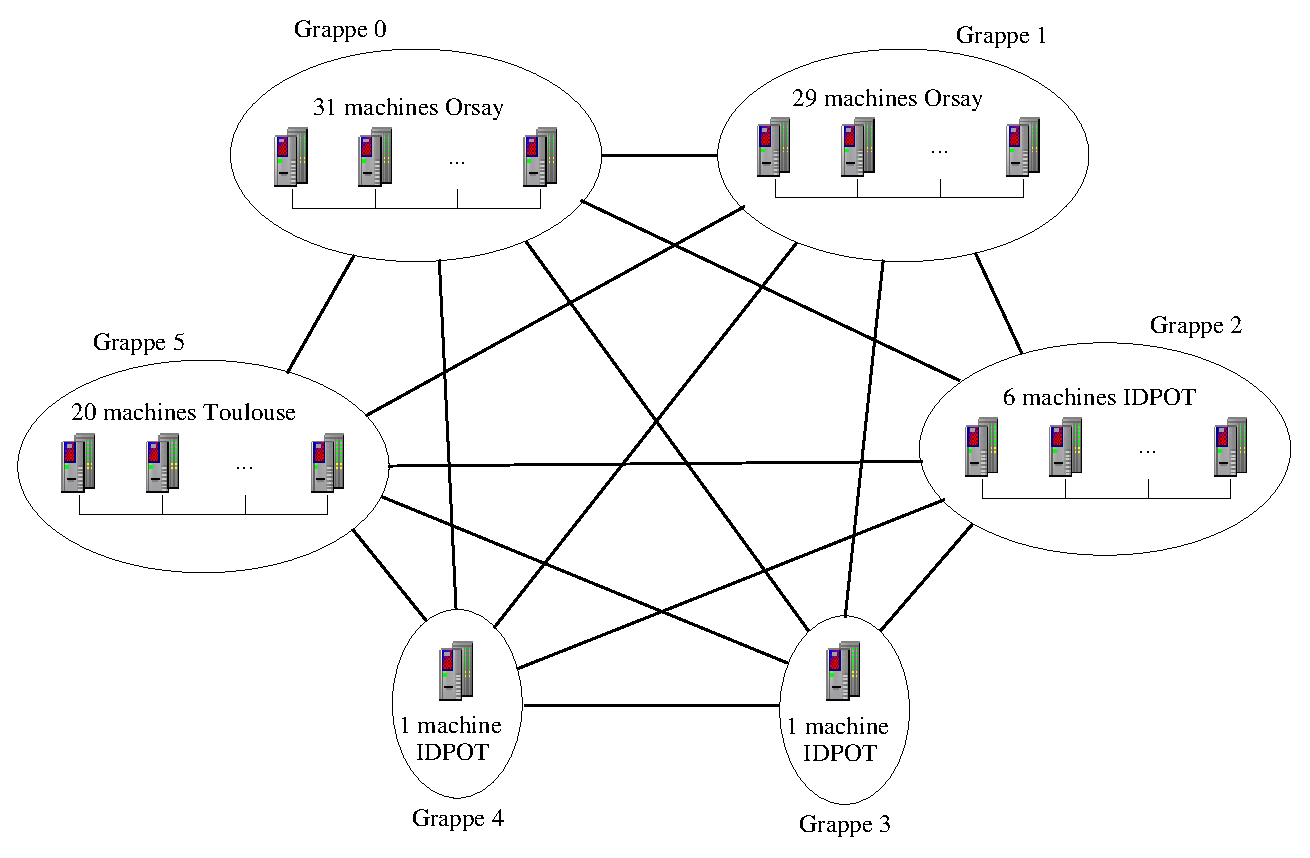
\includegraphics[width=0.75\linewidth]{images/Grid/Bcast/case1/grappe-case1}
%		\par\end{centering}
%	
%	\caption{\label{Figure: Bcast Grille 88 machines}Grille de 88 machines utilisée
%		dans les expérimentations pratiques}
%	
%\end{figure}
%

%Pour obtenir cette répartition des machines, on a utilisé l'algorithme
%de Lowekamp avec une tolérance de 30\%. Alors que le Tableau \ref{Tableau: Latence grid 1}
%indique la latence entre deux sites différents ou entre deux machines
%d'un même site (à part les grappes qui ont une seule machine), nous
%constatons des variations importantes de performance pour le réseau
%IDPOT. En effet, la latence d'interconnexion entre les machines IDPOT
%varie entre de $35\,\mu s$ et $242\,\mu s$, selon les machines.
%Ces variations sont dues surtout à l'utilisation de deux types différents
%de carte réseau, qui ont des performances distinctes, conformément
%à ce que nous avons indiqué dans \cite{Barchet04b}.

%
\begin{table}
	\caption{\label{Tableau: Latence grid 1}Latence entre les différents sites
		(en microsecondes)}
	
	
	\begin{centering}
		{\footnotesize }\begin{tabular}{|c||c|c|c|c|c|c|}
			\hline 
			& {\footnotesize Grappe 0} & {\footnotesize Grappe 1} & {\footnotesize Grappe 2} & {\footnotesize Grappe 3} & {\footnotesize Grappe 4} & {\footnotesize Grappe 5}\tabularnewline
			\hline 
			& {\footnotesize 31 x Orsay} & {\footnotesize 29 x Orsay} & {\footnotesize 6 x IDPOT} & {\footnotesize 1 x IDPOT} & {\footnotesize 1 x IDPOT} & {\footnotesize 20 x Toulouse}\tabularnewline
			\hline
			\hline 
			{\footnotesize Grappe 0} & {\footnotesize 47.56} & {\footnotesize 62.10} & {\footnotesize 12181.52} & {\footnotesize 12187.24} & {\footnotesize 12197.49} & {\footnotesize 5210.99}\tabularnewline
			\hline 
			{\footnotesize Grappe 1} & {\footnotesize 62.10} & {\footnotesize 47.92} & {\footnotesize 12181.52} & {\footnotesize 12198.03} & {\footnotesize 12195.22} & {\footnotesize 5211.47}\tabularnewline
			\hline 
			{\footnotesize Grappe 2} & {\footnotesize 12181.52} & {\footnotesize 12181.52} & {\footnotesize 35.52} & {\footnotesize 60.08} & {\footnotesize 60.08} & {\footnotesize 5388.49}\tabularnewline
			\hline 
			{\footnotesize Grappe 3} & {\footnotesize 12187.24} & {\footnotesize 12198.03} & {\footnotesize 60.08} & {\footnotesize 0$^{*}$} & {\footnotesize 242.47} & {\footnotesize 5393.98}\tabularnewline
			\hline 
			{\footnotesize Grappe 4} & {\footnotesize 12197.49} & {\footnotesize 12195.22} & {\footnotesize 60.08} & {\footnotesize 242.47} & {\footnotesize 0$^{*}$} & {\footnotesize 5394.10}\tabularnewline
			\hline 
			{\footnotesize Grappe 5} & {\footnotesize 5210.99} & {\footnotesize 5211.47} & {\footnotesize 5388.49} & {\footnotesize 5393.98} & {\footnotesize 5394.10} & {\footnotesize 27.53}\tabularnewline
			\hline
		\end{tabular}
		\par\end{centering}{\footnotesize \par}
	
	\begin{centering}
		{\footnotesize {*} cette grappe contient une seule machine.}
		\par\end{centering}
\end{table}


%Les mesures ont été effectuées en utilisant un processus de la grappe
%0 comme racine, et leur résultat est présenté dans la Figure \ref{Figure: Bcast - Case1 - Mesure}.
%On a comparé ces résultats avec l'implémentation \og pure \fg{} MPI,
%qui utilise des arbres binomiaux, comme décrit dans le chapitre \ref{cha:Mod=0000E9lisation des comms collectives}.
%Les prédictions de performance ont utilisé les valeurs de \emph{gap}
%et \emph{latence} (conformément au modèle pLogP) mesurées lors de
%l'initialisation de l'application, à travers la procédure de découverte
%de topologie décrite dans le chapitre \ref{cha: topo MPI}. Cependant,
%afin de permettre une meilleure compréhension de l'interconnexion
%entre les grappes, nous présentons les mesures des paramètres pLogP
%entre chaque grappe dans l'Annexe \ref{Annexe_A}.

Le premier résultat à noter est la faible performance de la stratégie
Flat, même par rapport à l'implémentation par défaut de LAM-MPI. Cela
ne veut pas dire que la stratégie Flat est toujours moins performante
que les autres stratégies, mais indique que cette stratégie est trop
dépendante de la configuration du réseau, de l'ordre de représentation
des grappes et du processus racine.

Dans le cas des autres heuristiques, on observe des gains de performance
déjà très importants. L'heuristique BottomUp %, comme prévu par lessimulations, 
n'est pas aussi efficace que les autres heuristiques,
qui de leur côté, se comportent de manière très similaire.

%
\begin{figure}[h]
	\begin{centering}
		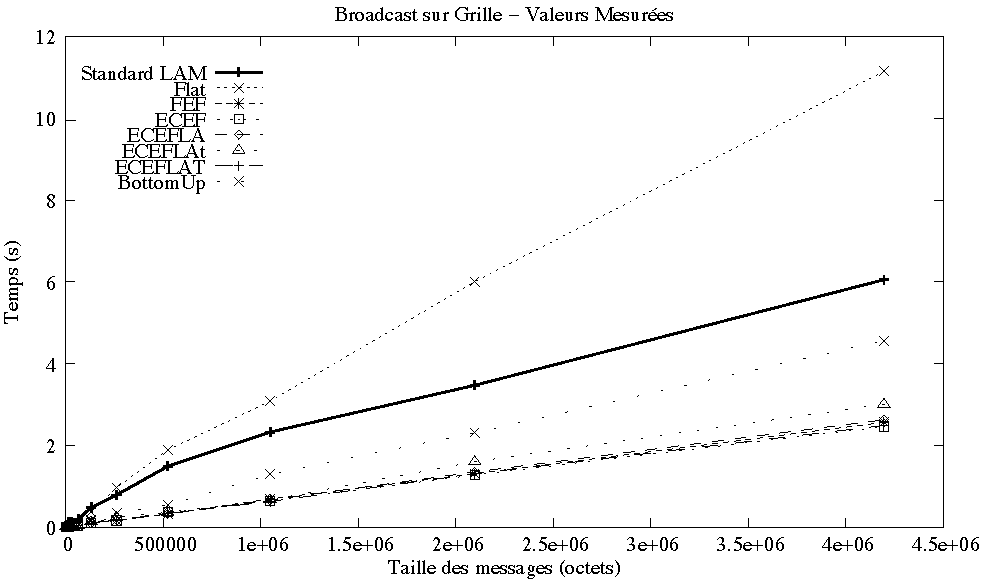
\includegraphics[width=0.8\linewidth]{images/Grid/Bcast/case1/comp}
		\par\end{centering}
	
	\caption{\label{Figure: Bcast - Case1 - Mesure}Performance du Broadcast sur
		une grille de 88 machines }
	
\end{figure}


Le faible écart observé entre les prédictions des heuristiques de
type FEF et ECEF-{*} est justifié surtout par le nombre réduit de
grappes, qui réduit le nombre de combinaisons possibles et fait converger
les résultats des différentes heuristiques. 

Pour mieux valider les résultats des expériences, la Figure \ref{Figure: Bcast case 1 predictions}
présente les temps prévus des différentes heuristiques. Ces temps,
calculés automatiquement par les heuristiques d'ordonnancement des
communications, donnent une meilleure indication de la fiabilité des
modèles par rapport aux résultats pratiques. Dans ce cas, nous observons
que les heuristiques de type FEF et ECEF-{*} ont des résultats très
rapprochés, certainement parce qu'elles ont obtenu le même ordonnancement
des communications. D'un autre côté, l'écart entre ces prédictions
et les résultats réels sont bien plus importants pour les heuristiques
FEF et ECEF-{*} que pour le BottomUp ou le Flat. Cela indique que
le coût du calcul de l'ordonnancement et le coût de la mise en oeuvre
de ces communications sont les facteurs les plus importants, et reflètent
l'augmentation de complexité d'une communication à couches multiples.

%
\begin{figure}[h]
	\begin{centering}
		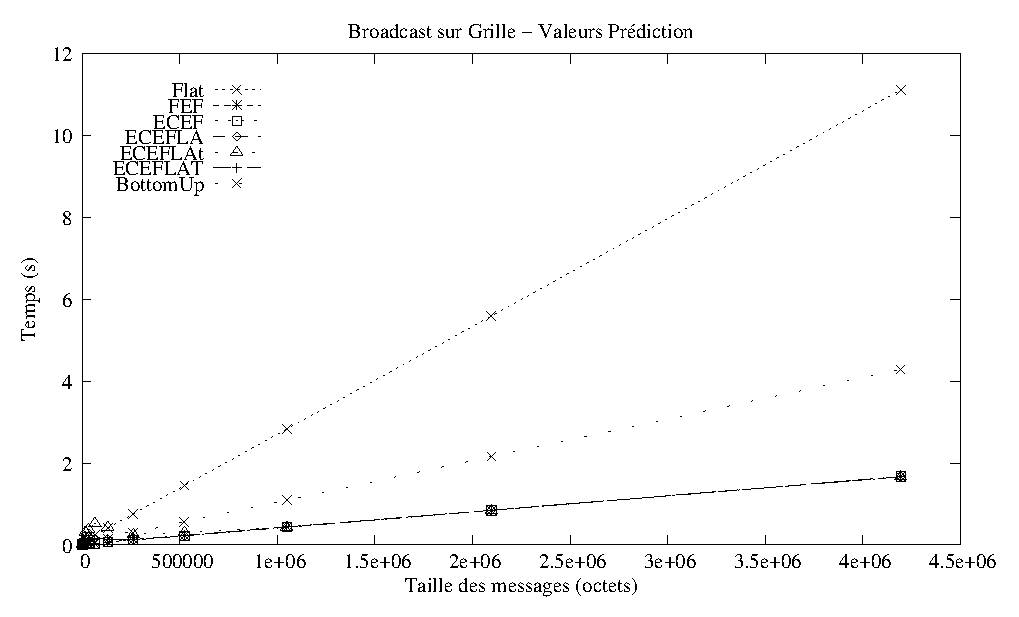
\includegraphics[width=0.8\linewidth]{images/Grid/Bcast/case1/simul}
		\par\end{centering}
	
	\caption{\label{Figure: Bcast case 1 predictions}Prédictions pour une grille
		avec 88 machines}
	
\end{figure}


%
%\subsubsection*{Cas No. 2}
%
%La deuxième expérience utilise 78 machines réparties entre les sites
%d'Orsay, Toulouse, Sophia-Antipolis et Grenoble (IDPOT). Alors que
%dans le cas précédent la majorité des machines appartenait à une seule
%grappe (Orsay), cette fois-ci nous avons utilisé des grappes plus
%équilibrées. En effet, nous avons utilisé 20 machines de la grappe
%GdX d'Orsay, 20 machines de la grappe de Toulouse, 19 machines de
%la grappe de Sophia-Antipolis et 17 machines de la grappe IDPOT.
%
%Comme dans le cas précédent, ces machines ont été regroupées en 6
%grappes homogènes différentes à l'aide de notre outil de découverte
%de topologie, qui implante l'algorithme de \emph{clustering} de Lowekamp.
%La disposition des grappes, représentée dans la Figure \ref{Figure: Bcast Grille 78 machines},
%est utilisée par la bibliothèque MagPIe pour établir la répartition
%des processus sur différentes grappes.
%
%%
%\begin{figure}[h]
%	\begin{centering}
%		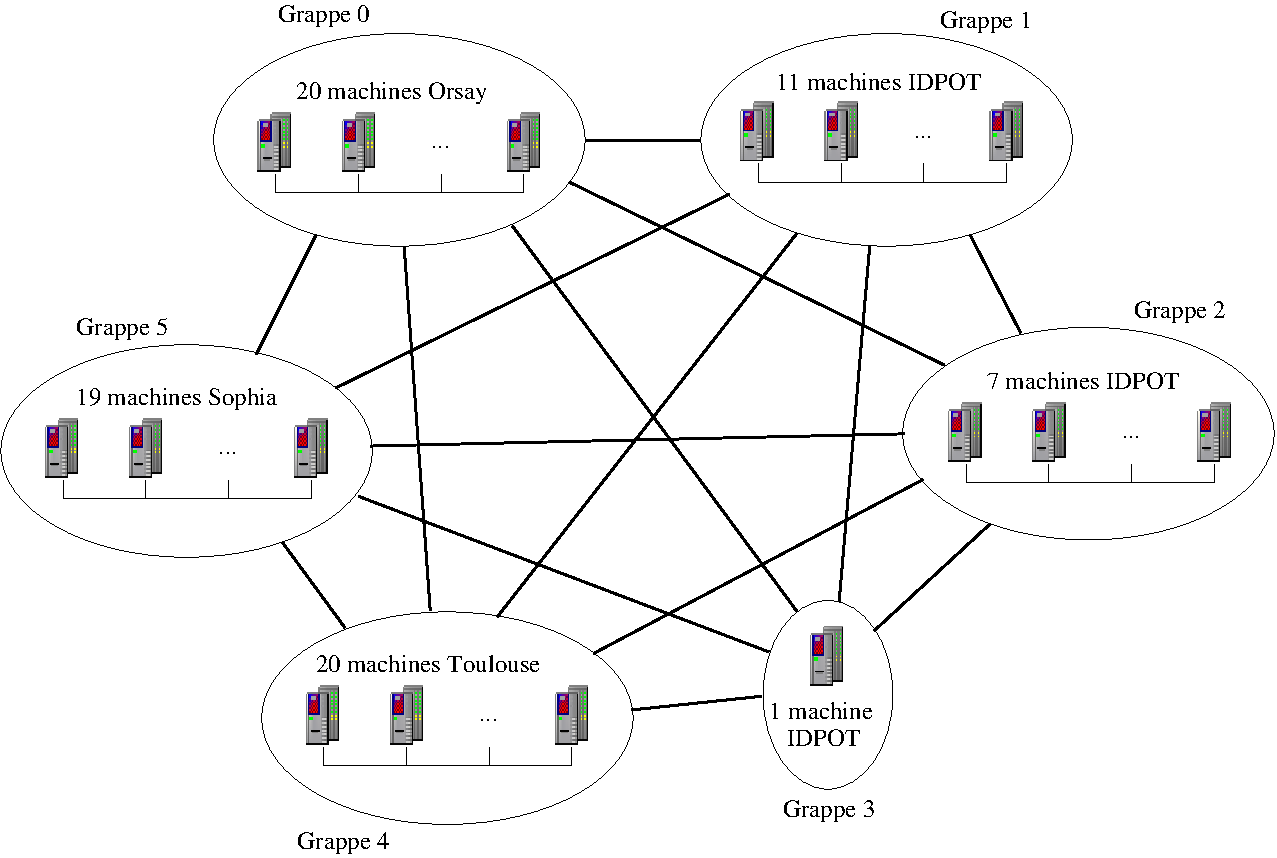
\includegraphics[width=0.75\linewidth]{images/Grid/Bcast/case2/grappe-case2}
%		\par\end{centering}
%	
%	\caption{\label{Figure: Bcast Grille 78 machines}Grille de 78 machines}
%	
%\end{figure}
%
%
%Les latences d'interconnexion entre les différents sites sont présentées
%dans le Tableau \ref{Tableau: bcast case 2 latences}. On observe
%que malgré la tolérance de 30\% utilisée par l'algorithme de \emph{clustering},
%la différence entre les machines IDPOT est suffisamment élevée pour
%forcer le regroupement des machines en plusieurs grappes.
%
%%
%\begin{table}
%	\caption{\label{Tableau: bcast case 2 latences}Latence entre les différents
%		sites (en microsecondes)}
%	
%	
%	\begin{centering}
%		{\footnotesize }\begin{tabular}{|c||c|c|c|c|c|c|}
%			\hline 
%			& {\footnotesize Grappe 0} & {\footnotesize Grappe 1} & {\footnotesize Grappe 2} & {\footnotesize Grappe 3} & {\footnotesize Grappe 4} & {\footnotesize Grappe 5}\tabularnewline
%			\hline 
%			& {\footnotesize 20 x Orsay} & {\footnotesize 11 x IDPOT} & {\footnotesize 7 x IDPOT} & {\footnotesize 1 x IDPOT} & {\footnotesize 20 x Toulouse} & {\footnotesize 19 x Sophia}\tabularnewline
%			\hline
%			\hline 
%			{\footnotesize Grappe 0} & {\footnotesize 48.39} & {\footnotesize 6577.49} & {\footnotesize 6586.49} & {\footnotesize 6592.51} & {\footnotesize 5211.94} & {\footnotesize 8602.73}\tabularnewline
%			\hline 
%			{\footnotesize Grappe 1} & {\footnotesize 6577.49} & {\footnotesize 35.52} & {\footnotesize 59.96} & {\footnotesize 59.96} & {\footnotesize 5387.48} & {\footnotesize 2736.56}\tabularnewline
%			\hline 
%			{\footnotesize Grappe 2} & {\footnotesize 6586.49} & {\footnotesize 59.96} & {\footnotesize 60.08} & {\footnotesize 79.51} & {\footnotesize 5393.98} & {\footnotesize 2740.26}\tabularnewline
%			\hline 
%			{\footnotesize Grappe 3} & {\footnotesize 6592.51} & {\footnotesize 59.96} & {\footnotesize 79.51} & {\footnotesize 0$^{*}$} & {\footnotesize 5405.78} & {\footnotesize 2745.98}\tabularnewline
%			\hline 
%			{\footnotesize Grappe 4} & {\footnotesize 5211.94} & {\footnotesize 5387.48} & {\footnotesize 5393.98} & {\footnotesize 5405.78} & {\footnotesize 26.94} & {\footnotesize 3630.51}\tabularnewline
%			\hline 
%			{\footnotesize Grappe 5} & {\footnotesize 8602.73} & {\footnotesize 2736.56} & {\footnotesize 2740.26} & {\footnotesize 2745.98} & {\footnotesize 3630.51} & {\footnotesize 35.04}\tabularnewline
%			\hline
%		\end{tabular}
%		\par\end{centering}{\footnotesize \par}
%	
%	\begin{centering}
%		{\footnotesize {*} cette grappe contient une seule machine.}
%		\par\end{centering}
%\end{table}
%
%
%Le résultat des mesures effectuées est présenté dans la Figure \ref{Figure: Bcast - case 2 - mesure}.
%On a comparé ces résultats avec l'implémentation \og pure \fg{} MPI,
%qui utilise des arbres binomiaux. Cette fois-ci, la disposition des
%grappes dans le fichier d'entrée de MagPIe a favorisé la stratégie
%Flat, qui a obtenu des performances similaires à celle des heuristiques
%plus élaborées. 
%
%%
%\begin{figure}[h]
%	\begin{centering}
%		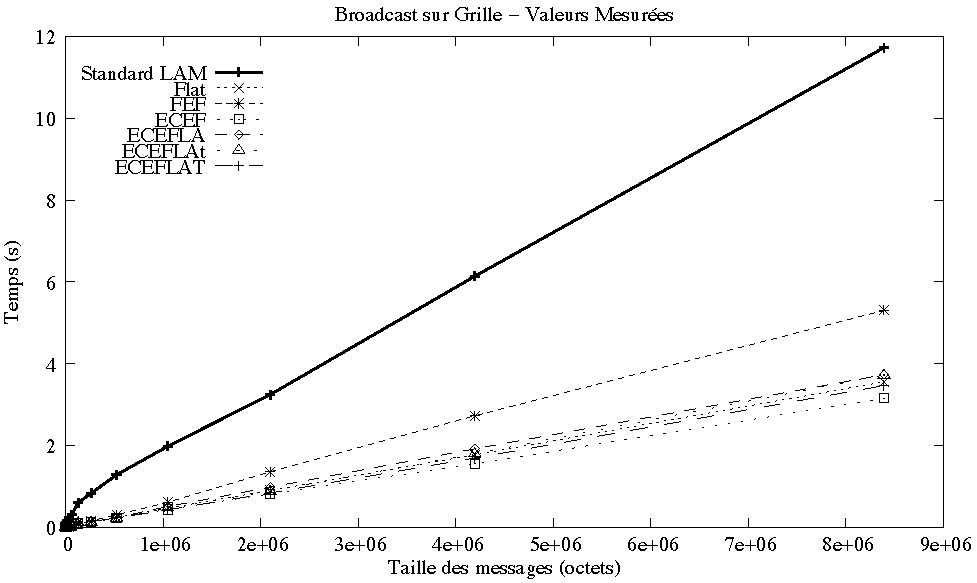
\includegraphics[width=0.8\linewidth]{images/Grid/Bcast/case3/comptipo3}
%		\par\end{centering}
%	
%	\caption{\label{Figure: Bcast - case 2 - mesure}Performance du Broadcast sur
%		une grille de 78 machines }
%	
%\end{figure}
%
%
%Dans un premier temps, l'analyse de la Figure \ref{Figure: Bcast - Case2 - zoom}
%indique que les heuristiques permettent un gain de performances important
%par rapport à l'algorithme en arbre binomial de la bibliothèque LAM-MPI.
%Parmi ces heuristiques, nous observons que les stratégies qui considèrent
%seulement la vitesse des liens, à l'instar de l'heuristique FEF, n'atteignent
%pas la meilleure performance. En effet, celle-ci est atteinte par
%les heuristiques de type ECEF, qui considèrent la disponibilité des
%processus, et non seulement la vitesse des liens. 
%
%Une remarque importante est que dans ce cas la stratégie Flat a obtenu
%des résultats similaires à ceux des meilleures heuristiques. Cela
%ne veut pas dire que l'heuristique Flat est optimale, mais seulement
%qu'elle est adaptée à l'ordre des grappes et au processus racine utilisé
%dans cette expérience. 
%
%%
%\begin{figure}[h]
%	\begin{centering}
%		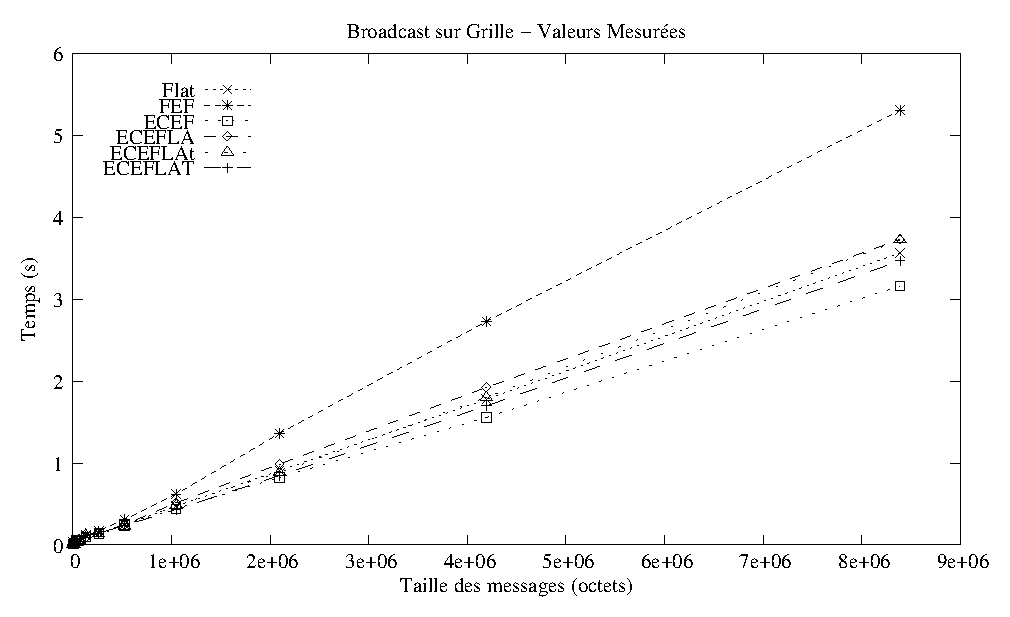
\includegraphics[width=0.8\linewidth]{images/Grid/Bcast/case3/comptipo3-zoom}
%		\par\end{centering}
%	
%	\caption{\label{Figure: Bcast - Case2 - zoom}Détails des performances des
%		heuristiques pour le Broadcast}
%	
%\end{figure}
%
%

\subsection{Considérations sur l'opération MPI\_Bcast }

Si dans un premier temps l'analyse des trois cas d'étude permet la
validation des certaines prédictions faites à travers la simulation
de différents environnements réseau, son apport le plus important
est l'observation du comportement des implémentations des heuristiques. 

Les trois situations étudiées ont notamment mis en évidence l'importance
du processus racine et de la répartition des processus sur des différentes
grappes sur la performance des stratégies plus simples. En effet,
la performance de la stratégie Flat est fortement liée à l'ordre de
représentation des grappes répartition, généralement fournie par l'utilisateur.
De surcroît, la stratégie Flat utilise toujours le même ordre de diffusion,
indépendamment du rang du processus racine. Au contraire, les heuristiques
les plus élaborées construisent des arbres de diffusion adaptés à
chaque situation, ce qui rend possible un gain de performance plus
important, surtout quand le rôle de \emph{racine} est alterné entre
plusieurs processus.

D'ailleurs, les simulations indiquent que la performance des stratégies
simples, comme le Flat, supportent très mal l'augmentation du nombre
de grappes interconnectées. Ceci met en cause l'efficacité de ces
stratégies dans un futur proche. Ainsi, nous croyons que, même si
la grille compte un nombre réduit de grappes, l'utilisation d'une
heuristique un peu plus élaborée, comme par exemple l'heuristique
ECEFLA-T, offre le meilleur rapport coût-bénéfice-robustesse.




\section{Bilan et Perspectives}

Dans ce chapitre nous avons présenté une stratégie efficace pour identifier
et découper les réseaux en grappes logiques homogènes. La présence
des hétérogénéités réduit la précision des modèles de communication
utilisés pour optimiser les communications collectives. Le \emph{framework}
proposé réussi à obtenir des paramètres de connectivité par un coût
très faible, à partir du regroupement d'informations obtenues indépendamment
dans chaque grappe. Notre approche, validée par des tests pratiques,
démontre que la découverte de topologie peut se faire de façon rapide
et précise. Associé à des modèles de prédiction de performance, le
découpage des grappes s'avère essentiel à l'optimisation des primitives
de communication collective, spécialement pour celles structurées
en multiples couches. De plus, ce \emph{framework} peut être étendu,
de manière à détecter aussi la présence de machines multiprocesseur,
information importante pour l'optimisation des communications.

Toutefois, la découverte de topologie a aussi des applications avec
d'autres domaines que le calcul parallèle. En effet, nous avons travaillé
au début de cette thèse avec l'application de la topologie sur les
algorithmes repartis comme la Diffusion Totalement Ordonnée. Ainsi,
l'Annexe \ref{cha:topo FT} montre comme la connaissance de la topologie
du réseau peut être utilisée pour augmenter la performance des algorithmes
repartis, réputés peu performants.




\chapter{L'hétérogénéité des Données}

% !TeX spellcheck = fr_FR
\begin{resume}

Le \textit{big data} a remis en évidence plusieurs défis pour les systèmes distribués, notamment les fameux "\textit{big V's}" : volume, variété, vitesse. Alors que le volume de données est plus ou moins simple d'être géré et que la vitesse dépend à la fois des ressources et des algorithmes, la variété des données est devenue l'un des points clé dans l'intégration des systèmes d'information\footnote{{\scriptsize \url{http://sloanreview.mit.edu/article/variety-not-volume-is-driving-big-data-initiatives/}}}. S'attaquer à cette hétérogénéité des données devient de plus en plus un défi pour le développement d'applications. 

Sans avoir l'ambition de proposer des solutions nouvelles pour la gestion de la variété de données, ce chapitre présente nos efforts visant à spécifier une plateforme documentaire garantissant un accès transparent à différentes sources d'information, indépendamment de la nature des données (fichiers, flux, bases de données, etc.). Cette spécification repose sur un ensemble d'éléments dédiés à l'indexation, à la recherche et à l'accès aux données. Également, la spécification s'occupe des mécanismes d'interconnexion et de coordination entre les éléments de la plateforme. Grâce à une organisation hiérarchique, cette plateforme a l'avantage de pouvoir être déployée sur une grande variété d'infrastructures.  

La majorité des travaux présentés dans cette partie résultent du travail de thèse de Thierno Ahmadou Diallo, effectuée sous la co-direction de Olivier Flauzac (Université de Reims Champagne Ardenne), de Samba Ndiaye (Université Cheikh Anta Diop, Sénégal) et moi-même. Ces travaux on fait l'objet de publication de deux journaux (\cite{Steffenel2015-Grappes,Steffenel12f}) et quatre conférences (\cite{Steffenel2014-CARI,Steffenel13a,Steffenel13c,Steffenel12d}).



\end{resume}

\section{Introduction}

La gestion de données à grande échelle est un problème récurrent autant dans les domaines scientifiques que dans le monde de l'entreprise. Malgré les constantes avancées en matière de capacité des mémoires et disques, l'utilisation d'un seul dispositif de stockage n'est plus une option vu que l'accès concurrent, la fiabilité, la consommation énergétique et le coût sont des obstacles au développement des systèmes. C'est pour cette raison que les chercheurs et développeurs se sont tournés depuis longtemps vers le développement de solutions de stockage distribué, afin de contourner ces limitations.

Dans les cas où les données peuvent être représentés sous la forme de fichiers, les solutions de type NAS/SAN, réseaux P2P et aussi le stockage dans des infrastructures de type (\textit{clouds}) représentent des choix technologiques capables d'offrir un stockage à grande échelle pour un coût raisonnable. Ces choix concernent aussi les bases de données de type relationnelle ou NoSQL, mais dans ce cas l'accès aux données requiert toujours une entité (pseudo)centralisée capable d'agréger et de présenter les données (ce qui n'exclut pas le traitement parallèle des requêtes). 

À travers différentes stratégies, ces solutions distribuées proposent des solutions transparentes à l'augmentation des besoins de stockage, tout en offrant suffisamment de garanties pour assurer la consistance et la pérennité des données. Aujourd'hui, l'utilisation de solutions de stockage de fichiers sur un NAS/SAN ou sur le \textit{cloud} est devenue aussi courante que l'utilisation de disques ou clés USB, une fois que les ressources potentiellement illimités offerts par les réseaux P2P ou les infrastructures de type \textit{cloud} présentent plusieurs avantages en ce qui concerne le coût, la disponibilité et l'utilisation des ressources physiques. Cependant, ces solutions peuvent aussi présenter des inconvénients liés à la vitesse d'accès et à la sécurité des données ; la solution à ces inconvénients est encore loin d'être garantie et dépend majoritairement des solutions propriétaires proposées par les fournisseurs des services de stockage. Un autre aspect à considérer est la compatibilité entre les systèmes : si certaines APIs rendent la manipulation des fichiers relativement simple, l'intégration d'autres représentations de données est moins évidente. Nous considérons qu'un système de gestion de données doit être capable aussi d'accéder à des requêtes sur une base de données, des flux de données ou encore faire appel à des Web services, le tout d'une manière uniforme et transparente pour l'utilisateur.

C'est dans le but de proposer une architecture unifiée pour les données et les services que nous avons présenté la spécification de la plateforme GRAPP\&S (\textit{GRid Applications and Services}), une architecture générique pour l'agrégation de données et services. Ce framework a été conçu de manière à intégrer de manière transparente les données de type fichier mais aussi les bases de données, les flux (audio, vidéo, données de capteurs et de l'Internet des Objets), les services Web et le calcul distribué. À travers une structuration hiérarchique basée autour du concept de "communautés", GRAPP\&S rend possible l'intégration de sources de d'information disposant de protocoles d'accès hétérogènes et des règles de sécurité variés.

\section{L'Architecture GRAPP\&S \label{SEC:GRAPPES}}

\subsection{Définitions\label{sec:Definitions}}
Pour la définition de l'architecture GRAPP\&S nous considérons un modèle de communication représenté par un  graphe non orienté  et connexe $G = (V, E)$, où $V$  désigne  l'ensemble  des  n{\oe}uds  du système et $E$ désigne l'ensemble des liens de communications qui existent entre les n{\oe}uds. Le modèle utilisé pour notre système est étudié dans \cite{Chalopin06}. Deux n{\oe}uds $u$ et $v$ sont dits adjacents ou voisins si et seulement si ${u, v}$ est un lien de communication de $G$. ${u_i, v_j} \in E$ est un canal bidirectionnel connecté au port $i$ pour $u$ et au port $j$ pour $v$. Donc les n{\oe}uds $u$ et $v$ peuvent mutuellement envoyer ou recevoir des messages en mode asynchrone. 

Un message $m$ en transit est noté $m(id(u), m', id(v))$ où  $id(u)$  est  l'identifiant du n{\oe}ud qui envoie le message, $id(v)$ est  l'identifiant du n{\oe}ud de réception, $m'$ indique le contenu du message. Chaque n{\oe}ud $u$ du système a un identifiant unique $id$ et  dispose de deux primitives : \texttt{send(message)} et \texttt{receive(message)}. Par soucis de clarté, nous introduisons quelques définitions.

%\newdef{definition}{Definition}
\begin{definition}Un n{\oe}ud  est  défini  comme  étant une  capacité de calcul, de stockage, avec  des moyens et des canaux de communications.\end{definition}

\begin{definition}Une donnée  brute  est  un flux  d'octets qui peut être  sous  différentes formes : une base de données objets ou  relationnelle, un fichier (texte et hypertexte, XML), un flux (vidéo, audio, VoIP),  des  requêtes  de  base  de données ou des résultats issus d'un calcul/service.\end{definition}

\subsection{Communication et les Réseaux \textit{Overlay}}
Le modèle de communication présenté en Section \ref{sec:Definitions} est suffisamment générique pour ne pas inférer sur la manière dont les messages sont effectivement livrés, se limitant uniquement à la définition des propriétés de communication bidirectionnelles entre deux vertex. Pour cette raison, l'architecture de GRAPP\&S peut s'appuyer sur n'importe quel un réseau de communication \textit{overlay} qui garantit une communication bidirectionnelle fiable et qui permet d'explorer différents chemins de communication pour chaque arête dirigée (réseau routé). Ceci donne une plus grande liberté d'implémentation et d'adaptation à l'environnement d'exécution, vu que les opérations send/receive peuvent être implémentées de différentes façons, selon les capacités de communication des n{\oe}uds. Dans ce cas, trois scénarios principaux peuvent être considérés : 
\begin{itemize}
	\item \texttt{Push}, où l'émetteur est capable d'envoyer un message directement au destinataire ;
	\item\texttt{Pull}, où le récepteur cherche régulièrement des messages en attente (ce modèle est fréquemment utilisé dans le cas des réseaux derrière un NAT/pare-feu) ; et 
	\item\texttt{Proxy}, où les voisins doivent passer par un n{\oe}ud intermédiaire afin d'échanger des messages (par exemple, grâce à un \textit{middleware} \textit{publisher/subscriber}). 
\end{itemize}
Dans ces trois scénarios, il est toujours possible d'établir un voisinage direct ou partiel entre les processus, ce qui est compatible avec le modèle par graphes connectes dirigés et qui répond donc aux besoins de l'architecture GRAPP\&S. 


\subsection{Éléments de l'Architecture GRAPP\&S}

Afin de présenter notre architecture, nous introduisons dans un premier temps quelques notations. Une communauté ($C_i$) est une entité autonome, qui regroupe des n{\oe}uds qui peuvent se communiquer et qui partagent une propriété définie : même localisation, même autorité d'administration (des serveurs distants appartenant à la même entreprise, par exemple) ou même domaine d'application (base de données métier, par exemple). Une communauté contient un seul processus \textit{Communicator} ($c$) et au moins un processus \textit{Ressource Manager} ($RM$) et un \textit{Data Manager} ($DM$) et ces processus sont organisés de façon hiérarchique dans une communauté. L'interconnexion entre différentes communautés C se fait grâce à des liens de voisinage point-à-point entre les processus Communicator.

\subsubsection*{Communicator (\textit{c})}
Le n{\oe}ud \textit{Communicator} (\textit{c}) joue un rôle essentiellement lié au transport d'informations et à l'interconnexion entre différentes communautés, comme par exemple lors du passage de messages à travers des pare-feu. C'est le point d'entrée de la communauté, et il assure sa sécurité vis-à-vis de l'extérieur, grâce à l'établissement de \textit{Service-Level Agreements} (SLAs) avec les autres communautés. De même, le communicateur coordonne la sécurité intérieure de la communauté, et peut modifier ses politiques d'accès grâce à des décisions prises au sein de la communauté \cite{Steffenel12a}. Un n{\oe}ud \textit{c} dispose d'un identifiant unique (ID) à partir duquel on construit les identités des autres n{\oe}uds de la communauté. Ce n{\oe}ud ne stocke pas de données et ne fait pas d'indexation.

\subsubsection*{Ressource manager (\textit{RM})} 
Les processus \textit{Ressource Manager (\textit{RM})} assure l'indexation et l'organisation des données et services dans la communauté. Ils reçoivent les requêtes des utilisateurs et assurent leur prétraitement. Les n{\oe}uds \textit{RM} participent à la recherche de données dans la communauté. Pour des fins de tolérance aux fautes et performance, les informations indexées par les \textit{RM} peuvent être redondantes et/ou partiellement distribuées (DHTs, par exemple). Afin de rendre plus performante la coordination des RMs, nous préconisons l'élection d'un RM désigné (voir section \ref{SEC:Community}).

\subsubsection*{Data manager (\textit{DM})} 
Les processus \textit{Data Manager (\textit{DM})} interagissent avec les sources de données, qui peuvent être dans différents supports tels que les bases de données (objet ou relationnelle), les documents (texte/XML/multimédia), des flux (vidéo, audio, VoIP), des données issues de capteurs ou encore une service hébergé dans le \textit{cloud}. 
Un n{\oe}ud DM est un service qui dispose des composants suivants : 
\begin{enumerate}
	\item[\textit{(i)}] une interface (proxy) adaptée aux différentes sources de données (disque dur, serveur WebDAV, FTP, base de données, stockage sur \textit{cloud} type Dropbox, etc.) et reliée à ceux-ci par un protocole de connexion spécifique au type de donnée, par exemple JDBC, ODBC, FTP, etc ;
	\item[\textit{(ii)}] un gestionnaire de requêtes qui permet d'exprimer des requêtes locales ou globales ; et 
	\item[\textit{(iii)}] un gestionnaire de communication qui permet au n{\oe}ud \textit{DM} de communiquer avec le n{\oe}ud \textit{RM} auquel il est connecté. 
\end{enumerate}

\section{Gestion de la Communauté\label{SEC:Community}}

GRAPP\&S peut être déployé dans plusieurs types d'architecture selon le placement des n{\oe}uds. Dans le modèle de placement (\textit{i}), les n{\oe}uds peuvent être regroupés dans une seule machine physique (voir Figure \ref{fig:noeuds}a). C'est l'exemple typique d'une machine d'un particulier, qui souhaite héberger une communauté de l'architecture. Le placement des n{\oe}uds sous cette forme peut être justifié par sa simplicité à mettre en {\oe}uvre lors de sa phase d'implémentation, en utilisant les concepts d'héritage et de polymorphisme. Les n{\oe}uds sont interconnectés par des sockets, des solutions RPC pour qu'ils puissent communiquer par message dans les deux sens entre deux n{\oe}uds. 

\begin{figure}
	\centering
	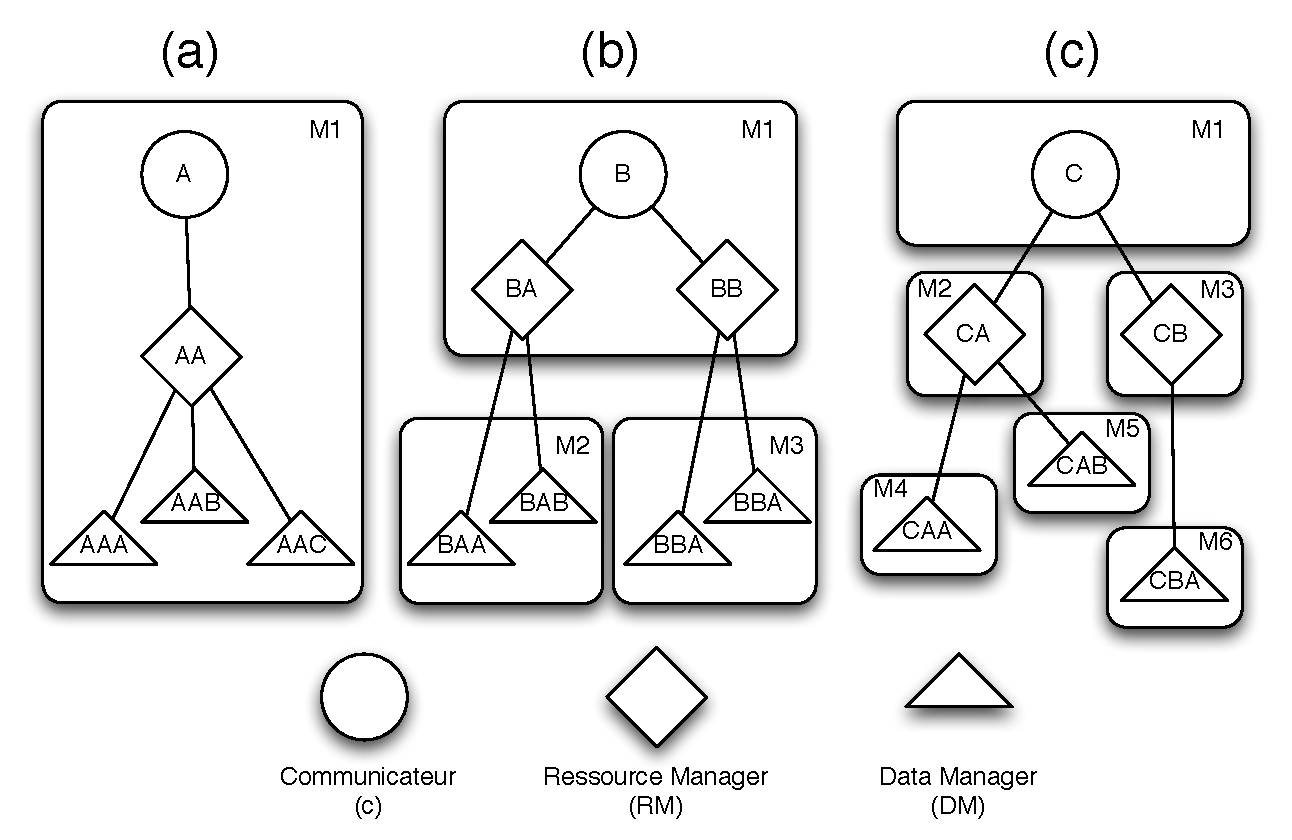
\includegraphics[width=0.85\linewidth]{img/noeuds.pdf} 
	\caption{Organisation des n{\oe}uds (a) dans une machine, (b) dans un \textit{cluster} et (c) dans un réseau\label{fig:noeuds}}
\end{figure}

Dans (\textit{ii}) les n{\oe}uds sont organisés dans une ferme de serveurs telle qu'un \textit{cluster}, ce qui est caractéristique des réseaux HPC (Figure \ref{fig:noeuds}b). Finalement, (\textit{iii}) les n{\oe}uds peuvent être regroupés s'ils partagent une même propriété de localisation ou d'administration (voir Figure \ref{fig:noeuds}c). Ceci est l'exemple d'un réseau formé par les n{\oe}uds d'une entreprise ou d'un laboratoire de recherche. 

Chaque n{\oe}ud de GRAPP\&S a un identifiant (ID) unique. Les adresses IP ou MAC ne sont pas des identifiants suffisamment précis car ils ne permettent pas d'identifier de manière unique les différents n{\oe}uds qui peuvent résider sur une même machine (par exemple, un $RM$ et plusieurs $DM$). De plus, l'utilisation des adresses IP ou MAC ne garantit pas une identité unique, vu que les adresses IP privés peuvent être réutilisées tout autant que les adresses MAC. En effet, l'utilisation massive de la virtualisation commence à poser des problèmes vis-à-vis de la réutilisation des adresses MAC, posant aussi des problèmes au niveau du le déploiement des réseaux IPv6\footnote{\url{http://tools.ietf.org/html/draft-gont-v6ops-slaac-issues-with-duplicate-macs-00}}. Ainsi, nous préconisons l'utilisation d'un mécanisme d'adressage inspiré par JXTA [8]. Dans le cas de GRAPP\&S, chaque n{\oe}ud dispose d'une chaîne unique $ID_{local}$ de 128bits, sous la forme "\texttt{urn:nom\_communaute:uuid:chaine-de-bit}". L'expression de l'adressage hiérarchique se fait par la concaténation des IDs sous forme de préfixe, c'est à dire., l'ID du n{\oe}ud $c_i$ est équivalent à son $ID_{local}$, l'ID du n{\oe}ud $RM_i$ est formé par $ID_{c_i}/ID_{RM_i}$, et l'ID du n{\oe}ud $DM_i$ présente la forme $ID_{c_i}/ID_{RM_i}/ID_{DM_i}$.

Un avantage de l'utilisation d'un modèle d'adressage propre à GRAPP\&S est que cela le rend indépendant du modèle d'adressage du réseau \textit{overlay} sur lequel GRAPP\&S est implémenté. Ainsi, deux communautés GRAPP\&S implémentées sur des \textit{middlewares} différents (FreePastry\footnote{\url{http://www.freepastry.org}} et Phex\footnote{\url{http://www.phex.org}}, par exemple) seront toujours compatibles, une fois la connexion établie entre leurs \textit{communicator}. 

\subsection{Gestion des N{\oe}uds}
La topologie du réseau change fréquemment à cause de la mobilité des n{\oe}uds. Nous travaillons dans l'hypothèse où les tout n{\oe}ud qui arrive dans le réseau est initialement un n{\oe}ud DM. Selon les conditions de l'environnement où ce n{\oe}ud se trouve, il peut se voir attribuer des rôles supplémentaires et "monter" dans la hiérarchie.

\subsubsection*{Connexion d'un n{\oe}ud}

Quand un n{\oe}ud $DM$ arrive dans le réseau, il dispose de deux moyens pour trouver un n{\oe}ud $RM$ sur lequel il peut se connecter :
\begin{itemize}
	\item Si le n{\oe}ud $DM_i$ connait un ou plusieurs n{\oe}uds $RM$, il envoie un message de diffusion \texttt{Hello()} et collecte toutes les identités des n{\oe}uds $RM$, qu'il garde dans un tableau ordonné par l'identifiant. Il peut ainsi se connecter au n{\oe}ud \textit{RM} qui a l'identifiant le plus grand. Si ce dernier se déconnecte, alors le $DM_i$ le supprime du tableau et se connecte au n{\oe}ud $RM$ suivant ; 
	\item Si par contre le n{\oe}ud $DM$ ne connait aucun n{\oe}ud $RM$, il doit effectuer une découverte sur le réseau local (par exemple, grâce à un multicast) ou contacter un service d'annuaire qui peut indiquer l'identifiant d'un n{\oe}ud $RM_i$. Comme la manière de trouver le n{\oe}ud $RM_i$ dépend de l'implémentation, elle n'est pas précisée dans notre architecture.
\end{itemize}
Finalement, si aucune tentative de connexion à un n{\oe}ud $RM$ (et par extension, un n{\oe}ud \textit{c}) ne réussit, le n{\oe}ud $DM$ a la possibilité de former sa propre communauté. Il assume ainsi les trois rôles $c$, $RM$ et $DM$, jusqu'à ce que d'autres n{\oe}uds le rejoignent. À ce moment, une élection pourra avoir lieu afin de redistribuer les rôles entre les n{\oe}uds.

\subsubsection*{Déconnexion d'un n{\oe}ud} 

Les n{\oe}uds peuvent subir des déconnexions volontaires ou des involontaires (pannes). Comme le cas des déconnexions volontaires est trivial, nous nous concentrons ici sur les déconnexions involontaires.

Entre deux niveaux hiérarchiques, les pannes peuvent être détectées soit par des messages périodiques de type \textit{Pull} (aussi connu comme \textit{heartbeat}), à la demande par des messages \textit{Push} (\textit{ping-pong}) \cite{Chandra96} ou encore en s'appuyant sur un mécanisme propre au \textit{middleware} \textit{overlay}. Pour les n{\oe}uds appartenant à un même niveau hiérarchique, la surveillance peut aussi se faire grâce à un mécanisme de passage de jetons "de service". Cela permet non seulement l'allégement du mécanisme de détection (il suffit de surveiller son prédécesseur et son successeur) comme permet la diffusion rapide des informations à l'ensemble des n{\oe}uds.

Pour la mise en place d'un mécanisme générique de détection de défaillances, nous préconisons une procédure en deux étapes. 
Tout d'abord, chaque n{\oe}ud dispose d'une liste de voisins \{$N_1,…,N_n$\} composée des n{\oe}uds en contact direct (par exemple, un $RM_i$ est en contact avec son $c$, ses $DMs$ et ses voisins $RM_{i-1}$ et $RM_{i+1}$. À cette liste de voisins est associé une liste de temporisateurs d'attente \{$ta_1,…,ta_n$\}. 

Lorsque aucun message du n{\oe}ud $N_k$ n'est reçu jusqu'à l'expiration du temps $ta_k$, une suspicion de défaillance est levée et doit être vérifiée auprès d'un deuxième n{\oe}ud qui est aussi en contact direct avec le n{\oe}ud suspect. Ainsi, si la suspicion concerne le n{\oe}ud $c$, un n{\oe}ud $RM_i$ interroge son voisin direct $RM_{i+1}$ avec un message jeton initialisé à \texttt{faux}. Si $RM_{i+1}$ a reçu un message du n{\oe}ud $c$ avant l'expiration de son temps d'attente $ta_c$, $RM_{i+1}$ modifie la valeur du jeton à \texttt{vrai} et retourne le message jeton à son émetteur $RM_i$. Ceci signifie (indirectement) que le n{\oe}ud $c$ n'est pas déconnecté et le n{\oe}ud $RM_i$ peut envoyer à nouveau un message au n{\oe}ud $c$. Si par contre $RM_{i+1}$ n'a pas été contacté récemment par $c$, il fera suivre un jeton la valeur \texttt{faux} qui, grâce au passage du jeton, alertera tous les n{\oe}uds $RM$ \{$RM_1,…,RM_n$\} de la défaillance de $c$.

De manière similaire, si un n{\oe}ud $c$ suspecte un n{\oe}ud $RM_k$, il peut demander confirmation à $RM_{k+1}$. Évidemment, cette procédure générique peut s'adapter aux différentes situations telles qu'un n{\oe}ud qui contient un $RM$ et plusieurs $DM$. Dans ce cas, le mécanisme de détection peut être allégé pour mieux répondre aux caractéristiques du n{\oe}ud. 

À la suite de la confirmation d'une défaillance, les n{\oe}uds concernés doivent \textit{(i)} mettre à jour leurs informations (liste de voisin, tableaux d'index, etc.) et éventuellement (\textit{ii}) procéder à l'élection d'un nouveau $RM$ (respectivement c) qui prendra en charge les éventuels $DM$ (ou $RM$) orphelins.  

\subsection{Coordination entre les N{\oe}uds}

Vu le caractère dynamique et volatile des réseaux informatiques, il est important de garantir la coordination entre les n{\oe}uds, notamment dans le cas des $RM$. Une manière simple et performante de faire ceci est de définir un n{\oe}ud avec des responsabilités étendues au sein de son groupe, ce choix étant fait par exemple grâce à une élection. 

L'élection d'un n{\oe}ud peut être nécessaire en deux situations : soit pour remplacer un n{\oe}ud défaillant et garantir la continuité du service (par exemple, lors de la panne d'un n{\oe}ud $c$), mais aussi pour simplifier la coordination entre les n{\oe}uds de même type, avec par exemple l'élection d'un $RM$ qui agirait comme "super-node" pour l'indexation de données et services. 

Il faut noter que la connaissance préalable des n{\oe}uds du niveau supérieur n'est pas obligatoire, vu que différentes techniques permettent d'obtenir les identifiants des autres n{\oe}uds. La méthode la plus simple consiste à utiliser directement le mécanisme d'adressage GRAPP\&S : étant indépendant du \textit{middleware} de communications, ce système d'adressage permet facilement de remonter la hiérarchie GRAPP\&S et de contacter d'autres n{\oe}uds (grâce au routage du réseau \textit{overlay}). Il suffit donc de remonter les niveaux de son propre identifiant ou de contacter d'autres n{\oe}uds dont on récolté les identifiants (ceux dont on a reçu des requêtes récemment, par exemple). Cette technique permet aussi de contacter d'autres \textit{communicators} $c_j$ et de réintégrer un réseau de communautés auprès la déconnexion involontaire de son \textit{communicator} $c_i$. En dernier recours, GRAPP\&S peut s'appuyer sur les éventuels mécanismes de découverte de topologie (broadcast/multicast) offerts par le propre \textit{overlay}.

Vu que le problème de la reconnexion au reste de la communauté peut être traité de manière plus ou moins simple au sein de la propre architecture GRAPP\&S, il est intéressant de se pencher sur les algorithmes d'élection eux-mêmes. Dans GRAPP\&S, nous préconisons un algorithme d'élection distribué inspiré des protocoles de routage OSPF et IS-IS \cite{rfc1142,rfc2328,ISISxOSPF}. En effet, les n{\oe}uds GRAPP\&S disposent d'un identifiant unique qui peut être utilisé de manière systématique par ces algorithmes d'élection. 

Le choix entre les algorithmes de IS-IS ou d'OSPF est plus lié aux préférences d'implémentation et à l'hétérogénéité des n{\oe}uds. En effet, l'algorithme d'élection de IS-IS est de type déterministe, où l'élu est toujours le n{\oe}ud avec le plus grand identifiant (appelé \textit{DIS - Designated IS}). Ce mécanisme est simple à implémenter et ne requiert pratiquement aucun échange d'informations car les n{\oe}uds disposent déjà d'une liste avec les identifiants de leurs voisins, il ne resterait que le coût associé à la prise de fonctions d'un n{\oe}ud élu à un rôle différent de celui qu'il occupait précédemment. L'inconvénient de cette technique est qu'un réseau avec un fort taux de volatilité peut occasionner des élections à répétition, soit lors de la déconnexion du leader, soit lors de la connexion d'un n{\oe}ud avec un identifiant prioritaire.

Dans les cas où la volatilité risque d'impacter la performance du réseau, il est possible d'utiliser un mécanisme non-déterministe comme celui d'OSPF \cite{ISISxOSPF}. Dans ce type d'algorithme, plus conservateur, le choix d'un leader (\textit{DR - Designated Router}) n'est nécessaire que si le leader actuellement en place disparaît. Ainsi, l'entrée de nouveaux n{\oe}uds dans la communauté a un impact moins important sur le fonctionnement du réseau.

 \section{Opérations dans GRAPP\&S\label{SEC:OPERATIONS}}

\subsection{Stockage et Indexation}

Le stockage de donnée dans le réseau GrAPP\&S fait intervenir les n{\oe}uds Data Manager $DM$, alors que les n{\oe}uds Ressource Manager $RM$ permettent d'indexer les données et les services. À la fin, chaque donnée est identifiée de manière unique grâce à l'identifiant du n{\oe}ud $DM$, auquel s'ajoute une extension contenant des informations et le type MIME des données. Ceci permet de franchir la barrière du simple "nom de fichier", et peut donc faire cohabiter des données statiques (fichiers), des données dynamiques (requêtes sur une base de données, résultats d'un calcul) et des données à caractère temporaire (flux voix ou vidéo, état d'un capteur, etc.). 

L'ajout d'une nouvelle donnée dans le réseau se fait ainsi : quand un n{\oe}ud $DM_i$ arrive dans le réseau, il se connecte à un n{\oe}ud $RM$ et publie les caractéristiques de ses données pour être indexées. Toute modification des données sur un $DM$ sont propagées au $RM$ auquel il est connecté, qui par la suite peut mettre à jour ces informations et les partager avec les autres $RM$. 

Cette propagation des informations peut prendre différentes formes selon les politiques utilisées lors de l'implémentation du réseau des $RM$. Une implémentation qui veut garder la simplicité pourra simplement garder un index local sur chaque $RM$, qui sera consulté lors d'une recherche. Au contraire, une implémentation souhaitant minimiser les échanges lors d'une recherche de données penchera sur l'utilisation d'un super-n{\oe}ud au sein des $RM$s ou d'un mécanisme de DHT. Il est aussi possible de favoriser la réplication des index et des données, ce qui exige une coordination entre les $RM$ afin de garder la cohérence des copies. Dans tous les cas, la surcharge des fonctionnalités d'un n{\oe}ud ("super-node") n'est pas une obligation dans notre structure mais simplement une spécificité pouvant être présente dans une implémentation donnée. 

\subsection{Recherche}
Quand un client cherche une donnée sur GRAPP\&S, il entre en contact avec un proxy $DM_i$, qui envoie une requête $Y$ contenant des informations qui identifient la donnée ou le service. Cette recherche dans une communauté de GrAPP\&S se fait par paliers, de manière à respecter l'organisation hiérarchique du réseau. La Figure \ref{fig:routage} illustre une partie de cette procédure de recherche : 
\begin{enumerate}
	\item Un n{\oe}ud $DM_i \in C_i$ envoie la requête a son n{\oe}ud $RM_i \in C_i$ ;
	\item $RM_i$ vérifie dans son indexe s'il y a parmi ses voisins un $DM$ qui contient la donnée recherchée ;
	\item Si oui, alors le n{\oe}ud $RM_i$ retourne au n{\oe}ud $DM_i$  une liste de n{\oe}uds $DM$ qui contiennent l'information recherchée ;
	\item Sinon, le n{\oe}ud $RM_i$ fait suivre la requête, soit directement aux voisins $RM_k \in C_i$ (si le mécanisme de communication le permet), soit à son n{\oe}ud $c_i \in C_i$ pour retransmission aux autres $RM_k \in C_i$ ;
	\item Quand un  n{\oe}ud $RM_k \in CM_i$ trouve la bonne réponse, alors la requête sera retournée au n{\oe}ud $DM_i$ émetteur en suivant le chemin inverse ;
	\item Si la donnée recherchée n'est pas dans la communauté $CM_i$, alors le $c_i$ fait suivre la requête vers d'autres communautés $CM_j$.  
\end{enumerate}

\begin{figure}
	\centering
	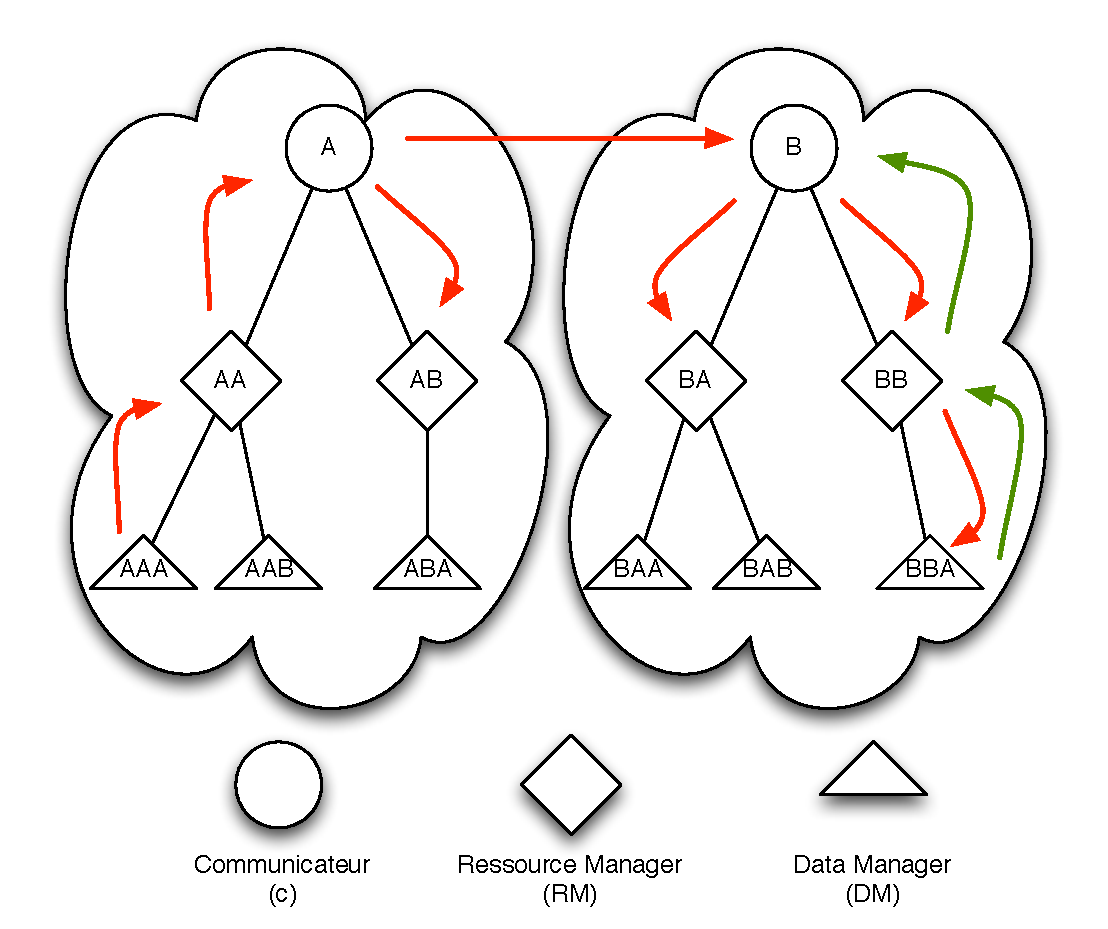
\includegraphics[width=0.8\linewidth]{img/Routage1.pdf} 
	\caption{Recherche d'une information dans GRAPP\&S et mécanisme de routage préfixé\label{fig:routage}}
\end{figure}

En cas de réussite, le client obtient l'identifiant du n{\oe}ud $DM_x$ responsable par la donnée. Dans ce cas, le client a deux possibilités pour accéder à la donnée, soit par connexion directe, soit par une connexion routée. Dans le cas de la connexion directe, le client fait une requête directe au n{\oe}ud $DM_x$ afin d'accéder à la  donnée. Comme le client peut se trouver dans un autre réseau qui ne permet pas l'accès directe à $DM_x$, la connexion peut se faire par routage interne dans GrAPP\&S. Cela se fait de la manière suivante :
\begin{itemize}
	\item Le client, par intermède d'un n{\oe}ud $DM_i$, envoie une requête \texttt{Req($id(DM_x, Y, id(c_i)$)} au n{\oe}ud communicateur $c_i$ ;
	\item  le n{\oe}ud $c_i$, par routage préfixé, envoie la requête \texttt{Req} vers le n{\oe}ud $RM$ qui a indexé la donnée ;
	\item  Ce dernier fait suivre la requête vers le n{\oe}ud $DM_x$ responsable de la donnée ;
	\item Une fois la donnée trouvée, le n{\oe}ud $DM_x$ retourne la bonne réponse au client en suivant le chemin inverse.
\end{itemize}   

Ce mécanisme de recherche hiérarchique empêche l'inondation des liens du réseau. La hiérarchisation permet de définir des chemins par lesquels transitent les requêtes et comme la connectivité logique de notre architecture est par définition de $(n-1)$, il suffit d'appliquer un algorithme de type PIF (\textit{Propagation of Information with Feedback} \cite{Seg83}) pour agréger les requêtes et réduire le nombre de messages d'une recherche.  


\section{Bilan et Perspectives}

Ce chapitre présente une spécification pour une plateforme distribuée basée sur les principes des réseaux hiérarchiques et visant l'établissement d'une base documentaire générique et extensible. Contrairement aux autres travaux que j'ai pu développer autour des systèmes distribués, l'objectif ici n'était pas celui de la distribution de tâches de calcul et leur gestion mais plutôt celui de l'indexation et de la recherche de documents et des sources d'information, le tout afin de minimiser l'hétérogénéité dans l'accès aux données. 

Bien que présente dans la spécification proposée, la coordination des n{\oe}uds fut d'abord conditionnée à la création et à la maintenance de réseaux de proximité pour cette gestion documentaire. La spécification de GRAPP\&S a aussi une qualité moins évidente, celle de l'indépendance vis-à-vis des technologies d'implémentation. De par sa propre organisation en "communautés", différentes instances de GRAPP\&S peuvent s'interconnecter et échanger des données, selon des politiques SLA définies par chaque partie.   

Également, la spécification de GRAPP\&S a permis une meilleure compréhension des différents mécanismes liés à la coordination et gestion des n{\oe}uds dans les réseaux hiérarchiques. En effet, la majorité de mes travaux repose sur une organisation uniforme du réseau où tous les n{\oe}uds possèdent les mêmes prérogatives ou au moins disposent de mécanismes de communication directe entre-eux. Dans le cas d'un réseau hiérarchique, les prérogatives dépendent du rôle joué par les n{\oe}uds, ce qui apporte des défis différents de ceux que je traite habituellement. 

Après avoir conclu la spécification de GRAPP\&S, les travaux de thèse de M Diallo se sont tournés vers la recherche et la description de scénarios d'application, comme par exemple dans le cas de l'\textit{e-learning}. Malheureusement, cela s'est fait au détriment de l'implémentation d'un prototype.  Certains concepts développées restent néanmoins présents dans les autres travaux que je développe, comme par exemple le concept de communautés. 

\chapter{L'hétérogénéité des Ressources de Calcul}

% !TeX spellcheck = fr_FR
\begin{resume}
La gestion de l'hétérogénéité des ressources peut être considérée sous plusieurs aspects. Les chapitres précédents ont donné des exemples de travaux dans lesquels l'hétérogénéité s'était concentrée sur les communications (Chapitre \ref{Chap:MPI}) ou sur le couple données-communication (Chapitre \ref{SEC:GRAPPES}). Dans ce chapitre nous nous concentrons sur un troisième socle, celui de l'hétérogénéité du calcul. Plus exactement, ce chapitre présente des travaux dont les contributions ont visé la prise en charge de l'hétérogénéité des ressources de calcul ou l'hétérogénéité des tâches de calcul, tous les deux résultant en une variabilité des temps d'exécution de tâches qui a dû être traitée et optimisée. Il est aussi important de remarquer que la communication et le stockage peuvent varier mais, dans ces cas, ils sont traités par des outils et mécanismes subjacents qui n'ont pas été la cible de nos travaux.

Ainsi, ce chapitre démarre avec la description d'une plate-forme de calcul destinée à l'exécution de problèmes d'amarrage moléculaire. Ce travail, développé dans le cadre de la codirection de thèse de Romain Vasseur, est un exemple d'application métier où l'environnement développée sert à déployer de manière distribuée une application déjà existante et dont le code source ne pourrait pas être facilement parallélisée. L'approche retenue a été composée d'une gestion distribuée d'instances de calcul sur un cluster, associée à un découpage plus fin du problème afin de multiplier les tâches de calcul et ainsi mieux utiliser les ressources disponibles.

La deuxième partie de ce chapitre décrit les efforts effectués dans le cadre du projet de collaboration international STIC-AmSud PER-MARE, dont l'un des objectifs a été de rendre la plateforme de calcul \textit{big data} Hadoop sensible au contexte et donc capable d'adapter la distribution des tâches de calcul en fonction des variations des ressources.

\end{resume}

\section{Hétérogénéité et Dynamicité des Ressources de Calcul} \label{sec:Guilherme}

La suite logicielle Apache Hadoop\footnote{\url{http://hadoop.apache.org/}} est très populaire dans le domaine du \textit{big data} et du calcul distribué. En effet, c'est l'un des outils pionniers dans le traitement de grandes masses de données grâce au support du paradigme de programmation \textit{MapReduce} \cite{Dean2008}. Bien que Apache Hadoop puisse être déployé sur des clusters composés de milliers de machines, ces ressources sont supposées être homogènes, sauf dans le cas d'une configuration spécifique de la part de l'administrateur. En effet, l'exécution des application \textit{MapReduce} dépend d'une bonne corrélation entre l'ordonnancement des tâches et les ressources alloués, or la présence de ressources hétérogènes ou dynamiques n'est pas suffisamment prise en charge par Hadoop. 

C'est pour cette raison que nous avons lancé le projet STIC-AmSud PER-MARE (Adaptive Deployment of MapReduce-based Applications over Pervasive and Desktop Grid Infrastructures - \cite{PER-MARE}) dont j'ai été l'idéalisateur et le coordinateur international. Le but de ce projet de collaboration international entre la France, le Brésil et l'Uruguay était de permettre le support aux applications \textit{big data} de type \textit{MapReduce} dans des environnements de type grid pervasif, c'est à dire, des environnements de calcul faiblement connexes marqués par l'hétérogénéité et par la volatilité des ressources \cite{3PGCIC}. Le projet PER-MARE était organisé autour de deux volets : d'un côté l'adaptation de la plate-forme Hadoop aux environnements pervasifs, et de l'autre le développement d'une solution de calcul distribué totalement répartie capable d'exécuter des applications de type \textit{MapReduce} (la plate-forme CloudFIT, traitée en section XXXX).
 %TODO mettre le lien vers la section cloudfit
 
Dans la suite de cette section on présentera donc l'architecture du framework Apache Hadoop et ses limitations concernant l'hétérogénéité des ressources. par la suite on verra les efforts effectués afin d'introduire des éléments liés au contexte dans l'ordonnancement des tâches, améliorant ainsi la performance et l'adaptabilité de la plate-forme. 



\section{Architecture et Ordonnancement dans Hadoop \label{subsec:ordoHadoop}}

Le framework Apache Hadoop est en réalité un écosystème assez important composé de presque une dizaine d'outils et services, allant de la gestion "bas niveau" des données et tâches de calcul à l'intégration avec des sources extérieures et le requêtage haut-niveau (parfois en imitant le langage SQL). Certains de ces outils ont été rajoutés au fil du temps grâce à des efforts de différents contributeurs (par exemple, le système de base de données HBASE développé initialement par Facebook). D'autres outils faisaient partie du projet dès son départ mais ont gagné un statut "projet" propre, comme par exemple le service ZooKeeper, responsable de la coordination distribuée fiable entre les n{\oe}uds et souvent au c{\oe}ur des efforts de tolérance aux fautes de Hadoop.

La plate-forme Hadoop elle aussi a subi des modifications au fil du temps. La version initiale (version 1.x) était extrêmement ancrée sur le paradigme \textit{MapReduce}, qui était le seul moyen d'utiliser la plate-forme. À partir de 2012 la version 2.x Hadoop devient une plate-forme plus générique, où l'on peut toujours exécuter des applications \textit{MapReduce} à côté d'autres applications. En effet, Hadoop devient surtout un gestionnaire de ressources qui aide à déployer et exécuter les tâches qui lui sont assignées.  

Au c{\oe}ur de la version 2.0 de Hadoop nous trouvons deux services principaux organisés chacun selon une architecture maître-esclave : le système de stockage distribué nommé HDFS (Hadoop Distributed File System) et le système de gestion des ressources nommé YARN (Yet Another Resource Negotiator). Les deux services présentent des composants jouant les rôles de maître ou esclave comme présenté en Figure \ref{fig:ArquiteturaHadoop} : les processus \textit{NameNode} et \textit{ResourceManager} correspondent aux rôles de maître dans HDFS et YARN, respectivement, et les processus \textit{DataNode} et \textit{NodeManager} correspondent aux parties esclaves. 

Nous pouvons observer aussi dans la Figure \ref{fig:ArquiteturaHadoop} la présence de deux autres composants appelés \textit{ApplicationMaster} et \textit{Containers} (conteneurs). L'\textit{ApplicationMaster} est un processus désigné pour effectuer l'ordonnancement des tâches de calcul d'une seule application, qui seront exécutées par des éléments \textit{Container} associés.  

\begin{figure}[!ht]
	\centering
	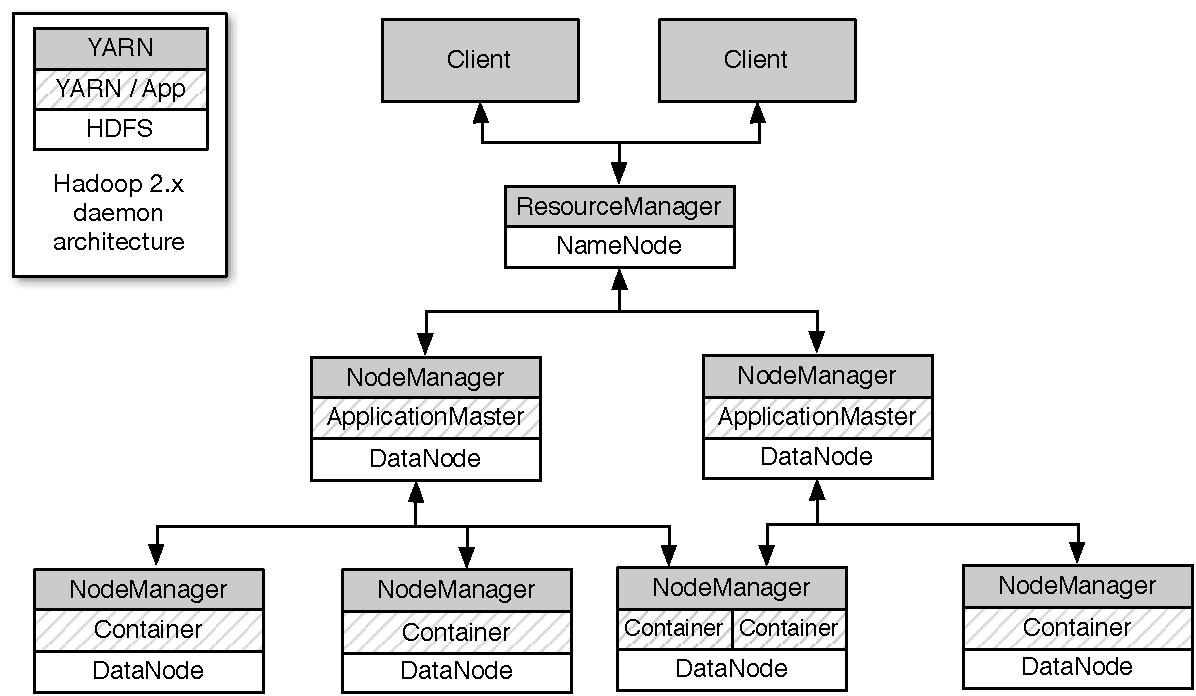
\includegraphics[width=0.85\linewidth]{img/HadoopArch.pdf}
	\caption{Architecture de base de Apache Hadoop 2.x}
	\label{fig:ArquiteturaHadoop}
\end{figure}


On observe donc que le framework Hadoop utilise deux niveaux d'ordonnancement. Les "jobs" représentent des instances avec une granularité plus grande, alors que les tâches représentent des instances de plus fin grain présentes au sein d'un job. 

L'ordonnancement au niveau des jobs est effectué par le \textit{ResourceManager}, la seule entité qui a une vue globale des ressources du système grâce aux informations envoyées par les \textit{NodeManager}. Grâce à ces informations, le \textit{ResourceManager} peut arbitrer la répartition des ressources entre les applications, en se basant sur différentes métriques telles que l'utilisation des ressources, l'équité, les contrats SLA, etc. Un \textit{ApplicationMaster} est ainsi détaché pour chaque application et devient responsable par l'ordonnancement et l'exécution des tâches de cette application par le biais des \textit{conteneurs}, des unités de calcul isolées et disposant d'un accès limité aux ressources (mémoire, CPU). 

Vu cette complexité, le \textit{ResourceManager} a été projeté de manière à pouvoir être optimisé selon contraintes et paramètres des utilisateurs, grâce à un mécanisme d'extensions. Toutefois, la plupart des utilisations répertoriées dans la littérature n'utilisent que les ordonnanceurs livrés avec Hadoop. Le plus simple de ces algorithmes d'ordonnancement est le \textit{Internal Scheduler}, une simple liste d'exécution où les jobs sont servis selon leur ordre d'arrivée (FIFO). Évidemment, cet algorithme n'est indiqué que pour les clusters où la compétition pour des ressources n'est pas un problème. 

Deux autres algorithmes sont souvent cités : l'algorithme \textit{Fair Scheduler} et l'algorithme \textit{Capacity Scheduler}. \textit{Fair Scheduler} utilise un mécanisme d'ordonnancement à deux niveaux pour effectuer un partage équitable entre des jobs de petite taille \cite{Hadoop}. \textit{Capacity Scheduler}, de son côté, a été créé pour l'utilisation de Hadoop dans un environnement où plusieurs partenaires contribuent afin de composer un grand cluster. En effet, le \textit{Capacity Scheduler} offre des garanties minimales d'accès aux ressources pour chaque partenaire, tout en permettant l'utilisation élargie du cluster lorsque des ressources se trouvent libres \cite{Hadoop}.

Les trois algorithmes cités ci-dessous illustrent des approches différentes pour la gestion des jobs, mais cela se fait uniquement par rapport à des facteurs tels que la disponibilité de ressources ou les politiques d'équité, sans jamais prendre en compte la dynamicité et l'hétérogénéité de l'environnement d'exécution. En effet, Hadoop considère que la gestion à grain fin de l'exécution incombe au  \textit{ApplicationMaster}, qui a une vue plus proche de l'application mais qui est aussi limité aux ressources que lui sont attribués au départ.

Malheureusement, le fonctionnement de l'\textit{ApplicationMaster} est peu documenté. Afin de combler ce manque d'information, nous avons analysé son code source et conduit des expériences pour comprendre ses politiques d'allocation des tâches (résultats publiés dans \cite{UBICOMM2014}). Ce que ressort est un simple mécanisme de remplissage des n{\oe}uds visant la proximité des tâches : on remplit un n{\oe}ud avec autant de conteneurs qu'il peut supporter, pour ensuite commencer re remplissage du prochain n{\oe}ud.   

Ceci nous a permis aussi d'observer que l'\textit{ApplicationMaster} se limite à répartir les conteneurs sans une véritable adéquation au contexte d'exécution. Toute connaissance sur la capacité des n{\oe}uds provient du \textit{ResourceManager}, la seule entité qui est alimentée avec ces informations. Ainsi, la modification des algorithmes d'ordonnancement dans le but d'inclure des informations de contexte doit se faire en étroite relation avec le \textit{ResourceManager}.



\section{Dynamicité des Ressources dans Hadoop} \label{sec:related}

La littérature propose différentes approches pour rendre Hadoop plus compatible avec les environnements hétérogènes. Des travaux comme \cite{Kumar2012}, \cite{Tian2009} ou \cite{Rasooli2012} assument que les applications \textit{MapReduce} sont exécutées régulièrement dans un environnement de "production", et que chacune des applications a des besoins spécifiques en CPU, mémoire, réseaux ou en stockage. Cette hypothèse considère donc la possibilité d'optimiser l'exécution des application en faisant la correspondance entre les besoins et les caractéristiques des ressources. De même, \cite{Isard2009} propose un algorithme d'ordonnancement où une fonction de coût basée sur un graphe "capacité-demande" permet l'ordonnancement des jobs.

Les travaux cités ci-dessus considèrent des ressources hétérogènes mais statiques et, une fois lancés, ces jobs ne sont plus "suivis" car l'environnement est supposé immuable. Une manière de rendre cet ordonnancement plus dynamique est d'incorporer des informations sur le déroulement des tâches. Par exemple, \cite{Zaharia2008} et \cite{Chen} essayent d'améliorer la distribution des tâches afin de réduire le temps de réponse dans des clusters de grande taille. Pour cela, \cite{Zaharia2008} utilise des heuristiques pour estimer la progression des tâches et ainsi décider s'il faut lancer des tâches spéculatives. Les tâches spéculatives sont des doublons (ré-soumissions) qui sont lancées lorsqu'il y a la soupçon qu'une tâche originale est retardée à cause d'un n{\oe}ud défaillant ou trop lent. Dans une ligne similaire, \cite{Chen} propose l'utilisation des traces historiques d'exécution afin d'aider cette décision. 


Une autre manière d'augmenter la performance passe par un meilleur placement des données et par l'utilisation de cette information pour le déploiement des jobs \cite{Xie2010}. En faisant un placement optimisé des données, on réduit les transferts de données occasionnés par le lancement de tâches spéculatives sur d'autres n{\oe}uds. Une approche similaire est présentée par \cite{Cavallo2015}, qui étudie les problèmes d'ordonnancement et répartition des données dans les clusters géographiquement distribués. Ainsi, ces auteurs présentent un mécanisme d'ordonnancement basé sur les ressources de calcul mais aussi sur le débit du réseau.  

Sans aucun paramètre supplémentaire, les mécanismes cités jusqu'à présent ont comme résultat un équilibrage de charge, obligeant les n{\oe}uds les plus rapides à travailler plus et les moins performants à exécuter moins de tâches. Une manière de rompre cette logique est utilisée par \cite{Sandholm2010},  qui permet d'influencer l'ordonnancement grâce à des profils d'exécution suggérés par l'utilisateur (par exemple, privilégier les n{\oe}uds lents si le job n'est pas prioritaire).  

Il faut observer cependant que la difficulté à adapter l'exécution de \textit{MapReduce} sur des environnements hétérogènes (et dynamiques) est en grand partie due à la conception même de la plate-forme Apache Hadoop, qui est très hiérarchique (voir Figure \ref{fig:ArquiteturaHadoop}). Certains travaux essayent de s'affranchir de ces barrières en développant d'autres plates-formes compatibles avec \textit{MapReduce} mais plus adaptées à l'a dynamicité des ressources.  L'utilisation de overlays P2P est ainsi un choix naturel, comme le montrent \cite{Marozzo2012} et \cite{Steffenel20151034}. Dans le système proposé par \cite{Marozzo2012}, les n{\oe}uds incarnent les différentes fonctions de l'architecture Apache Hadoop (NameNode, etc.) selon les besoins de l'application. Cependant, ce travail vise la tolérance aux fautes et n'explore pas les possibilités d'optimisation de l'ordonnancement des jobs et des tâches. 

L'approche adoptée par la plate-forme CloudFIT \cite{Steffenel20151034} est différente car même si elle repose aussi sur un overlay P2P, on n'essaye pas d'imiter le fonctionnement de Hadoop. CloudFIT est une plate-forme générique de calcul distribué, où des tâches Map et Reduce sont distribuées aux n{\oe}uds de façon opportuniste, selon un mécanisme "bag of tasks". Cette distribution est aussi guidée un ordonnancement guidé par le contexte des ressources et par des profils d'exécution fournis par les applications. Nous détaillerons le fonctionnement de CloudFIT dans le chapitre suivant.

Il faut aussi noter que, à l'exception de CloudFIT, les travaux cités précédemment ne tiennent pas compte de l'évolution des ressources au fil de l'exécution : les ressources sont décrites mais pas observées. Malgré la diversité de travaux sur l'importance de la prise en compte du contexte d'exécution \cite{Baldauf, Maamar, Ramakrishnan2014, Najar2015}, Hadoop reste essentiellement une plate-forme statique. Pour toutes ces raisons, une partie de notre travail au sein du projet STIC-AmSud PER-MARE a été d'intégrer les informations de contexte à l'exécution de Hadoop.

\section{Ordonnancement Orienté par le Contexte} \label{sec:desenv}

Comme indiqué dans la section \ref{subsec:ordoHadoop}, l'élément central de l'ordonnancement est le \textit{Resource Manager}. En effet, c'est grâce aux informations fournies par cet élément que les ordonnanceurs de Hadoop tels que le \textit{Capacity Scheduler} décident du démarrage et du placement des tâches. 

L'implémentation par défaut de Hadoop considère qu'un \textit{NodeManager} déclare ses ressources au \textit{ResourceManager} lors de sa connexion au réseau Hadoop, or la description de ces ressources est usuellement obtenue à partir de fichiers de configuration statiques. Afin de rendre cette information de contexte dynamique, nous devons mettre en place un mécanisme de capture de contexte et aussi permettre au \textit{NodeManager} de communiquer périodiquement ses ressources au \textit{ResourceManager}. 

Afin de modifier le moins possible le code de Hadoop, nous avons développé un module de capture de contexte qui peut être greffé à Hadoop et ainsi mettre à jour les informations sur les ressources disponibles. Les sous-sections suivantes détaillent le fonctionnement de ce module et aussi le mécanisme retenu pour son intégration à Hadoop.

\subsection{Le Collecteur de Contexte\label{sec:gestionnairecontexte}}
Par défaut, Hadoop obtient des informations sur les ressources des n{\oe}uds à partir de fichiers de configuration au format XML. Ces fichiers contiennent plusieurs paramètres, dont le nombre d'unités d'exécution (c{\oe}urs de calcul) et la capacité de la mémoire des n{\oe}uds. Une fois lues, ces informations ne sont pas mises à jour, sauf en cas de redémarrage du n{\oe}ud. Afin de rendre possible l'exécution de Hadoop dans un environnement pervasif, nous avons mis en place un mécanisme de collecte d'informations de contexte qui peut être utilisé pour ajourner la base de connaissances du \textit{ResourceManager}.

Ce collecteur de contexte a été développé dans le cadre du projet PER-MARE\cite{PER-MARE} et est structuré selon le diagramme de classes présenté en Figure \ref{fig:CollectorDiag} \cite{UBICOMM2014}. La capture des différents éléments de contexte se font grâce à l'API standard Java Monitoring API \cite{Oracle}, qui permet l'accès aux caractéristiques de la machine virtuelle Java et de la machine hôte. En effet, cela nous permet d'obtenir des informations de contexte telles que le nombre de processus (c{\oe}urs de calcul), la mémoire du système, ou la charge de ma machine. Le collecteur de contexte a été structuré avec un ensemble d'interfaces et de classes abstraites, ce qui permet de généraliser le processus de la collecte des données. De plus, en raison de sa conception, il est simple d'intégrer des nouveaux collecteurs et ainsi diversifier les informations de contexte.

\begin{figure}[!ht]
	\centering
	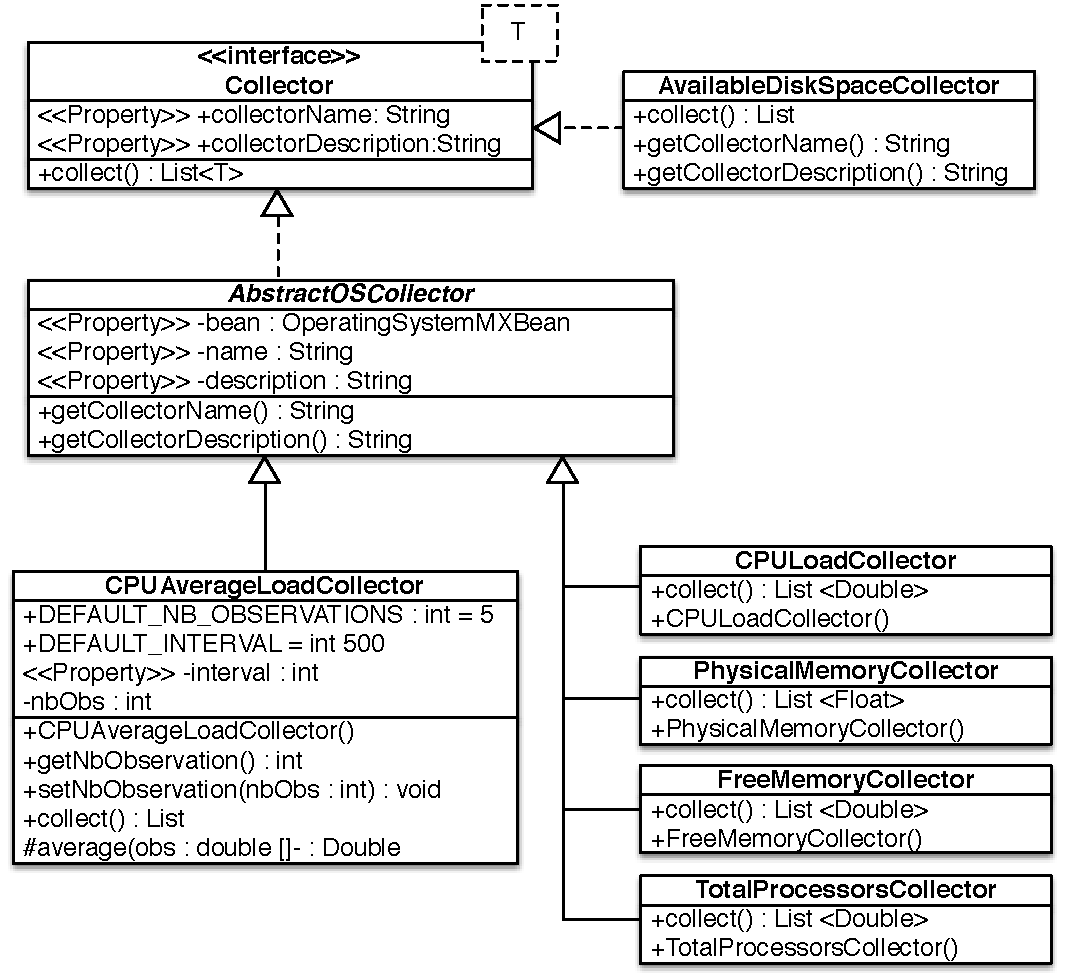
\includegraphics[width=0.75\linewidth]{img/CollectorUML2.pdf}
	\caption{Structure du collecteur de contexte}
	\label{fig:CollectorDiag}
\end{figure}

Cependant, il ne suffit pas de remplacer les fichiers de configuration XML par les informations du collecteur car ces informations resteraient statiques. Afin d'ajourner le \textit{ResourceManager}, il faut que le collecteur de contexte de chaque n{\oe}ud puisse communiquer son état au \textit{ResourceManager}, et cela à n'importe quel moment de l'exécution. Afin de rendre ceci possible, nous avons étendu les possibilités de communication entre le \textit{ResourceManager} et les \textit{NodeManager}, comme expliqué dans la section suivante.    

\subsection{Communication}
Dans l'architecture Hadoop, les informations de contexte collectées par les n{\oe}uds esclaves (\textit{NodeManager}) doivent être transmises au n{\oe}ud maître (\textit{ResourceManager}), qui sera en charge de l'ordonnancement. Au lieu de créer un mécanisme séparé, nous avons choisi d'intégrer cette communication au sein de l'API ZooKeeper \cite{Hunt2010}, qui fait partie de l'écosystème Hadoop. Dans notre cas, les services de ZooKeeper seront utilisés pour récupérer les informations de contexte et les rendre disponible auprès le \textit{ResourceManager}. 

\begin{figure}
	\centering
	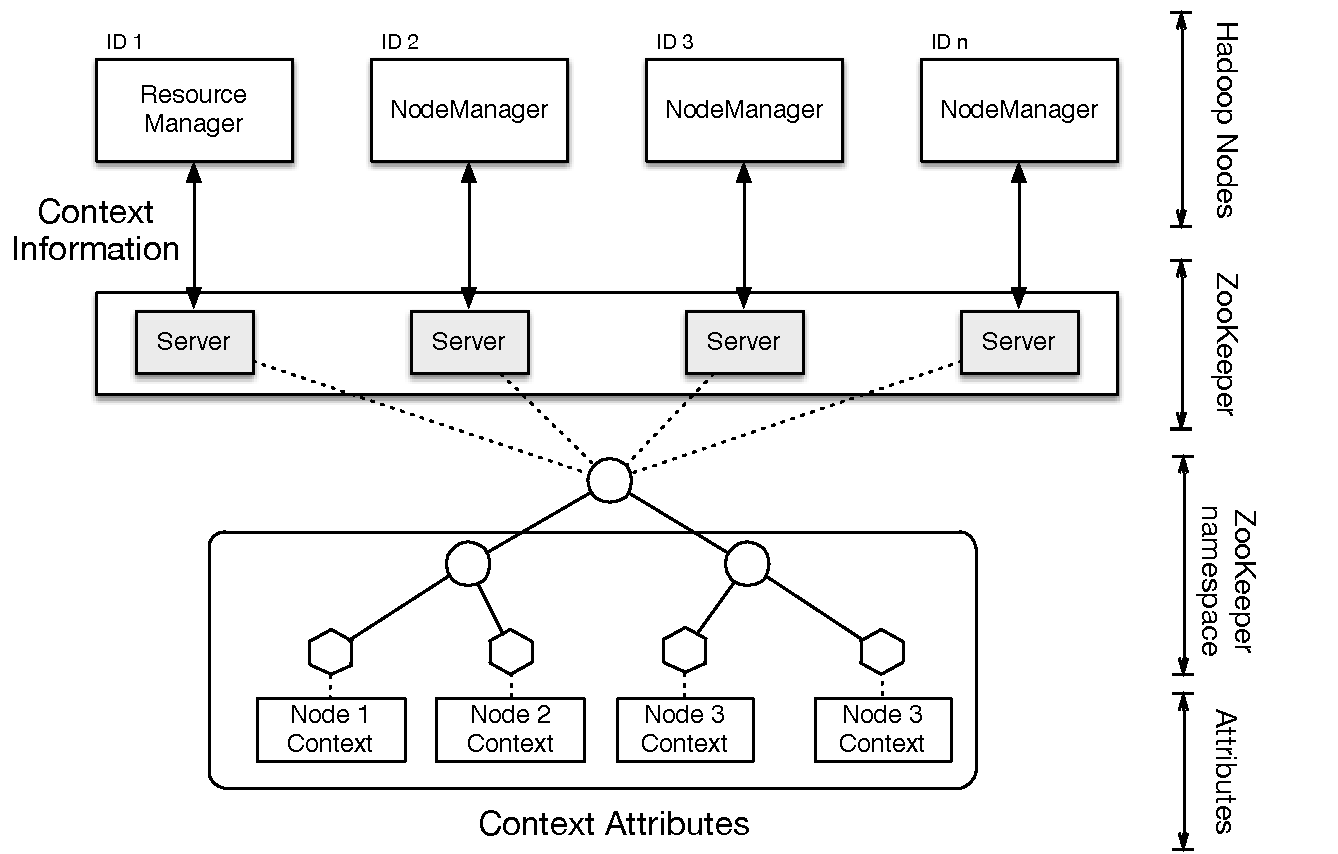
\includegraphics[width=1\linewidth]{img/Zookeeper} 
	\caption{Utilisation de ZooKeeper pour distribuer l'information de contexte\label{fig:zookeeper}}
\end{figure}


Comme illustré en Figure \ref{fig:zookeeper}, tous les esclaves (\textit{NodeManager}) exécutent une instance du service \textit{NodeStatusUpdater}, lequel collecte régulièrement les données sur la disponibilité des ressources (par exemple, à chaque 30 secondes). Si les ressources varient plus qu'un certain seuil/plafond, le tableau dans ZooKeeper sera mis à jour. Ce seuil/plafond est nécessaire car le système d'exploitation peut subir des légères variations des ressources (par exemple, la quantité de mémoire disponible) alors que ces variations n'ont pas un impact sur la capacité d'un n{\oe}ud. Ce mécanisme contribue aussi pour réduire la quantité d'informations échangées et évite trop d'événements qui pourrait impacter la performance de l'algorithme d'ordonnancement. 

De manière similaire, le maître (\textit{ResourceManager}) crée aussi un service pour surveiller les informations sur de ZooKeeper. Lorsque ZooKeeper détecte une modification des données, le maître sera notifié et pourra mettre à jour les informations utilisées par l'ordonnanceur. Les modifications apportées au code source du \textit{ResourceManager} et des \textit{NodeManager} est assez limitée, permettant son application sur différentes versions de Hadoop.

Dans la section suivante nous allons montrer les résultats de quelques expériences faites pour valider ce mécanisme.


\section{Évaluation Pratique} \label{sec:exper}

Afin d'évaluer l'impact de la prise en compte du contexte dans le cadre de l'ordonnancement des tâches, nous avons conduit une série d'expériences sur un petit cluster dédié. Cet environnement nous permet de contrôler les ressources disponibles et aussi ceux "observés" par le framework Hadoop, de manière à pouvoir mesurer l'impact d'une mauvaise détection et les avantages de l'adaptation au contexte. Dans les tests effectués, nous avons observé le comportement de Hadoop selon deux métriques, la ressource "mémoire disponible" et le nombre de c{\oe}urs de calcul (\textit{v-cores}). Ces paramètres sont toujours renseignés au \textit{ResourceManager} et font partie des principaux attributs utilisés par l'algorithme Capacity Scheduler. En effet, la mémoire totale disponible et le nombre de c{\oe}urs permettent la définition du nombre de tâches simultanées (conteneurs) qui peuvent être exécutées par un n{\oe}ud. Une mauvaise information peut donc créer une surcharge de la machine, affectant la performance.  

Pour la définition des scénarios d'exécution, nous avons travaillé avec l'hypothèse que la performance est dégradée si la mémoire disponible annoncée au gestionnaire de ressources est supérieure à celle réellement disponible. La situation contraire (plus de mémoire disponible que celle annoncée) n'impacte pas l'exécution d'une tâche. Ainsi, nous avons défini 4 situations d'exécution :

\begin{description}
	\item[Scénario A :] dans ce scénario "de contrôle" la mémoire disponible annoncée au gestionnaire de ressources correspond à la mémoire disponible. De même, le nombre de c{\oe}urs de calcul renseigné correspond au nombre de c{\oe}urs disponibles. Les ressources ne varient pas pendant l'exécution, ce qui peut être considéré comme le "best case". 
	\item[Scénario B :] dans ce cas, la mémoire disponible et le nombre de c{\oe}urs sont inférieurs à ceux annoncés. Cependant, elle ne sera pas mise à jour au niveau du gestionnaire de ressources, reproduisant ainsi le comportement par défaut de Hadoop. Comme l'ordonnanceur ne s'adapte pas, ceci peut être considéré comme un scénario "worst case".
	\item[Scénario C :] dans ce troisième cas, le collecteur de contexte est actif dès le départ et renseigne les ressources effectivement disponibles à chaque 30 secondes. Ainsi, quand l'application est lancée, l'ordonnanceur est au courant du contexte d'exécution et peut lancer les tâches conformément à ces ressources, sans surcharger les machines. 
	\item[Scénario D :] finalement, ce scénario représente une extension du Scénario C dans lequel l'exécution de l'application \textit{MapReduce} démarre avant la mise à jour du collecteur de contexte. De cette manière l'ordonnanceur est initialisé avec des informations incorrectes et doit s'adapter pendant l'exécution. Cette adaptation n'est pas immédiate car elle ne concerne que l'ordonnancement des tâches en attente, pas celle des tâches déjà en exécution.
\end{description}


\subsection{Benchmarks et Environnement de Tests}

Deux types différents d'application ont été utilisés comme benchmarks afin de vérifier l'impact de l'adaptation au contexte. Même si les applications \textit{big data} sont fortement dépendantes de l'accès mémoire, d'autres facteurs comme l'utilisation de la CPU ou les opérations d'entrée/sortie (I/O) sont aussi importantes. Pour cela, les deux applications choisies ont des profils différents par rapport à leurs besoins en mémoire, CPU et  I/O \cite{Benchmarks}, comme indiqué ci-dessous :
\begin{itemize}
	\item TeraSort: L'application TeraSort \cite{TeraSort2008} est une application destinée à effectuer le tri d'un grand ensemble de données. C'est un benchmark très populaire car les algorithmes de tri stressent la mémoire et la CPU au même temps qu'ils sollicitent l'I/O à cause des masses des données à trier ;
	\item TestDFSIO: Le benchmark TestDFSIO a été conçu spécifiquement pour étudier l'interaction de Hadoop avec HDFS, permettant la découverte de goulots d'étranglement au niveau du réseau d'interconnexion, du système d'exploitation et de la configuration Hadoop. Dans cette application, la mémoire et la CPU sont moins sollicitées.
\end{itemize}

Les deux benchmarks font partie de la plate-forme de tests HiBench \cite{HiBench}. Le tri TeraSort a été exécuté sur un ensemble de données de 15 GB, alors que TestDFSIO a été exécuté avec 90 fichiers de 250 MB chacun. Les différents scénarios ont été exécutés sur la plate-forme Grid'5000 \cite{g5k}. Nous avons configuré un réseau dédié avec 5 machines (dont une "maître" et quatre "esclaves"), chacune avec la configuration suivante : 2 Intel Xeon CPU E5420 @ 2.50 GHz (8 c{\oe}urs par n{\oe}ud) et 8 GB de mémoire RAM. Tous les n{\oe}uds exécutent Ubuntu-x64-12.04, avec JDK 1.7 et la distribution Apache Hadoop 2.5.1. 

L'analyse des performances se fait grâce à l'étude des fichiers de log de chaque tâche (conteneur), qui contiennent des informations sur le n{\oe}ud d'allocation, le moment de démarrage et le temps nécessaire pour l'exécution de chaque tâche. Nous avons choisi d'exécuter les tâches "maître" sur un n{\oe}ud séparé afin de ne pas surcharger les n{\oe}uds esclaves avec des activités de gestion de Hadoop. 

Finalement, afin d'émuler la réduction des ressources en mémoire et c{\oe}urs de calcul nécessaires aux scénarios B, C et D, nous avons choisi de réduire le nombre effectif de n{\oe}uds utilisés, une méthode drastique mais plus fiable que la limitation logicielle des ressources disponibles.

\subsection{Résultats\label{sec:5.4}} 

Les exécutions des benchmarks dans les différents scénarios sont représentées par les diagrammes de Gantt des Figures \ref{fig:gantts} et \ref{fig:DFSIO}, respectivement pour TeraSort et TestDFSIO. De même, les Tableaux \ref{tab:resumo} et \ref{tab:DFSIO} résument les données clés de ces expériences, avec le temps total d'exécution des tâches \textit{map}, le temps moyen d'exécution, l'écart type, le nombre de tâches \textit{map} et aussi le nombre de tâches spéculatives démarrées.  

\begin{figure*}[!ht]
	\centering
	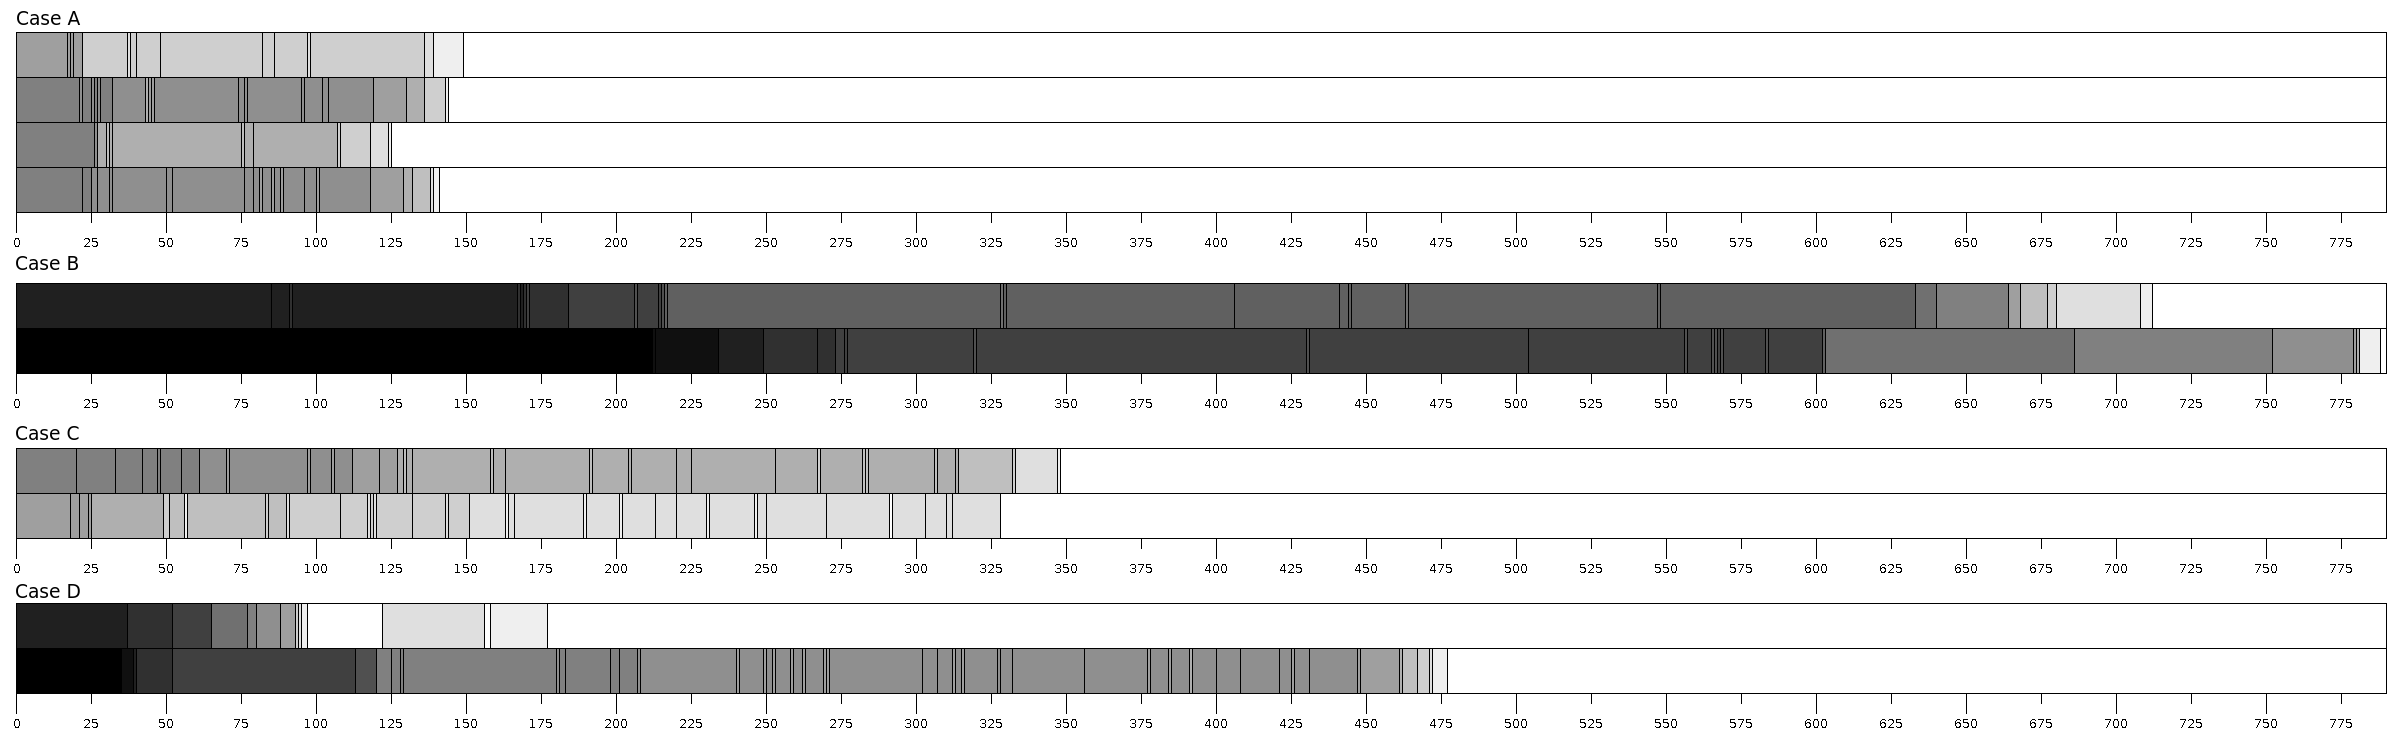
\includegraphics[width=1\textwidth]{img/todos}
	\caption{Diagramme de Gantt pour l'exécution de TeraSort}
	\label{fig:gantts}
\end{figure*}

\begin{figure*}[!ht]
	\centering
	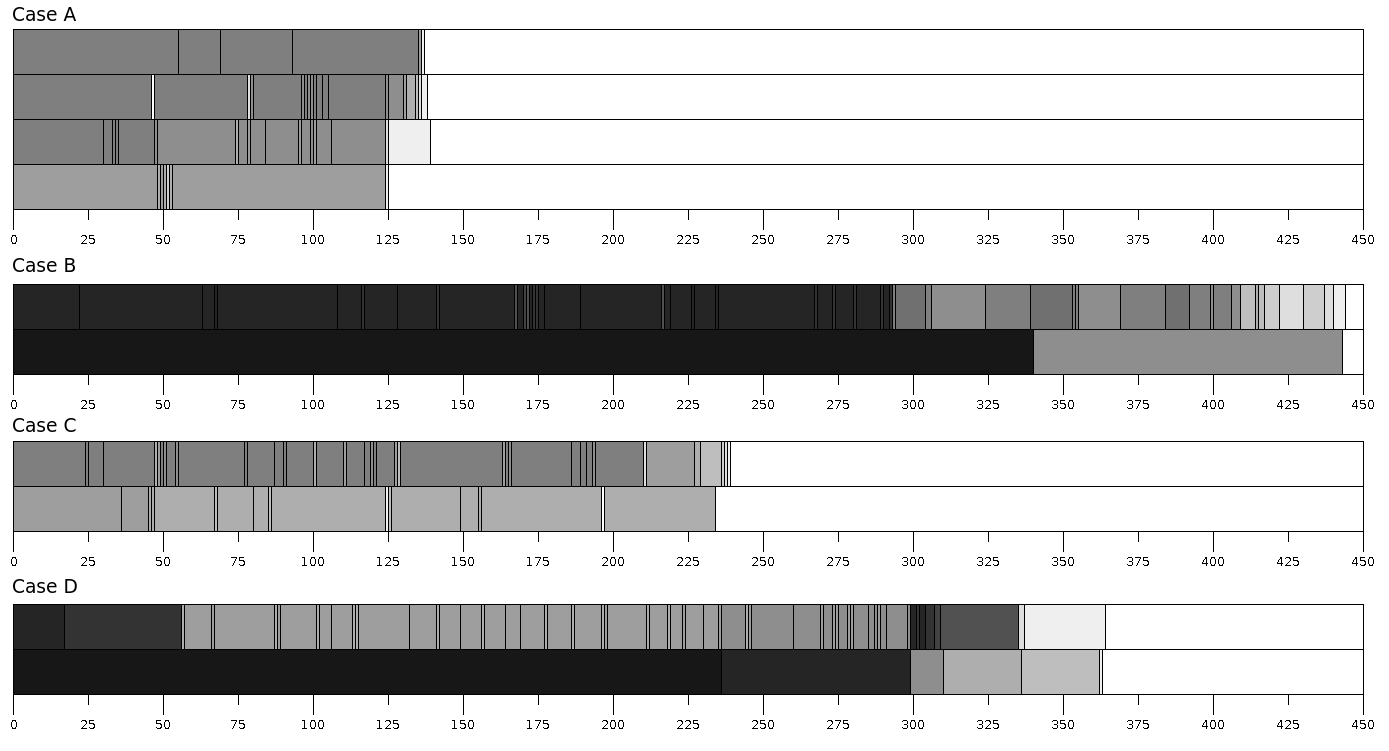
\includegraphics[width=1\textwidth]{img/todos-DFSIO}
	\caption{Diagramme de Gantt pour l'exécution de TestDFSIO}
	\label{fig:DFSIO}
\end{figure*}


\begin{table}
	\caption{Tableau récapitulatif de l'exécution de TeraSort} \label{tab:resumo}
	\centering
	\begin{tabular*}{0.6\hsize}{lllll} 
		\textbf{Scénario} & \textbf{A} & \textbf{B} & \textbf{C} & \textbf{D}\\
		\hline
		Temps total \textit{map} ({\it{s}}) & 149 & 788 & 348 & 477 \\
		Temps moyen ({\it{s}}) & 39.47 & 222.97 & 38.38 & 68.42 \\
		Écart type & 15.73 & 59.86 & 18.09 & 29.91 \\
		\# tâches \textit{map} & 76 & 76 & 76 & 76 \\
		\# tâches spéculatives & 2 & 1 & 3 & 1 \\
	\end{tabular*}
\end{table}

\begin{table}
	\caption{Tableau récapitulatif de l'exécution de TeraSort} \label{tab:DFSIO}
	\centering
	\begin{tabular*}{0.6\hsize}{lllll} 
		\textbf{Scénario} & \textbf{A} & \textbf{B} & \textbf{C} & \textbf{D}\\
		\hline
		Temps total \textit{map} ({\it{s}}) & 139 & 444 & 239 & 364 \\
		Temps moyen ({\it{s}}) & 38.95 & 85.01 & 32.20 & 81.62 \\
		Écart type  & 17.20 & 69.08 & 8.30 & 73.60 \\
		\# tâches \textit{map} & 90 & 90 & 90 & 90 \\
		\# tâches spéculatives & 0 & 9 & 0 & 1 \\
	\end{tabular*}
\end{table}


Pour les diagrammes de Gantt, chaque scénario est composé de 2 ou 4 lignes correspondant au nombre de n{\oe}uds utilisés. Comme indiqué précédemment, les scénarios B, C et D n'utilisent que la moitié des n{\oe}uds du scénario A afin de simuler la réduction des ressources. L'échelle de couleurs présent dans chaque ligne indique la surcharge des n{\oe}uds : plus sombre est le créneau, plus de conteneurs s'exécutent simultanément. De cette manière, un créneau "blanc" n'a aucun conteneur en exécution, alors qu'un créneau "noir" en contient 16 conteneurs (le double de la capacité d'un n{\oe}ud). Les séparations des créneaux indiquent soit le démarrage d'une tâche, soit une fin d'exécution, mais ne permettent pas de suivre le temps d'exécution d'une tâche précise. 

L'analyse des tableaux permet d'identifier certaines tendances. En effet, toutes les exécutions présentent un motif similaire quand on observe le temps total d'exécution : le scénario A est toujours le plus rapide, suivi de des cas C et D puis finalement  B. Nous observons aussi que les scénarios A et C ont les plus petits temps moyens et les plus petites variations de performance, indépendamment de l'application. Ceci s'explique par le fait que dans ces deux scénarios les n{\oe}uds ne sont jamais surchargés car l'ordonnanceur a des informations précises au moment du démarrage de l'application. Ceci s'observe aussi par la tonalité des créneaux, indiquant un nombre moins important de tâches en simultané. Le temps total d'exécution du scénario C est aussi deux fois plus important que celui du scénario A, une conséquence attendue à cause de la réduction des ressources. 

L'analyse du nombre de tâches spéculatives apporte aussi quelques renseignements. Dans le cas de TeraSort, tous les scénarios se comportent de manière similaire. Par contre, dans le cas de TestDFSIO le déploiement de tâches spéculatives ne se fait que lorsque le système est surchargé (notamment dans le scénario B). La raison pour cette différence vient des facteurs qui sont liés au lancement de tâches spéculatives : une tâche spéculative n'est lancée que seulement après le lancement de toute autre tâche "originale", et déclenchée seulement lorsque ces tâches sont en exécution depuis un certain temps (au moins une minute) et n'ont pas progressé autant que la moyenne des autres tâches du job. Dans le cas de TeraSort, les tâches dépendent autant de la mémoire que de la CPU et de l'I/O, et le recouvrement de ces besoins compense d'une certaine manière le manque d'une ressource. TestDFSIO, à l'opposé, s'appuie sur des ressources plus spécifiques et est donc plus enclin à la surcharge des n{\oe}uds. Et même dans les scénarios surchargés, l'utilisation d'un mécanisme de détection du contexte sur le scénario D permet à l'ordonnanceur de lisser la charge lors de la mise à jour des informations sur les ressources.

Il faut aussi pointer un détail concernant les diagrammes de Gantt. Dans tous les benchmarks il y a un n{\oe}ud qui semble moins chargé que les autres. Ceci n'est pas la faute à une mauvaise répartition de la charge mais plutôt à la présence de tâches \textit{reduce}, qui ne sont pas affichées dans les diagrammes. En effet, Hadoop permet le démarrage de tâches \textit{reduce} aussitôt un certain nombre de tâches \textit{map} a été complété, ce qui est le cas pour ces applications.

Le résultat de ces expériences démontre que l'utilisation d'un mécanisme de collecte et de mise à jour des informations de contexte permet l'adaptation de l'ordonnanceur Hadoop aux aléas d'une plate-forme d'exécution dynamique. La solution que nous avons proposé dans ce travail permet non seulement un gain de performance dans les scénarios avec risque de surcharge mais aussi impose très peu de modification au niveau du code source de Hadoop, rendant la solution suffisamment générique et intégrable aux différentes versions de ce framework. 


\section{Bilan et Perspectives} \label{sec:disc}

%TODO rajouter une note sur le travail avec Javier et Matias, après tout ça fait partie des choses faites avec Hadoop









\chapter{CloudFIT : un intergiciel pour le \textit{Fog Computing} et l'Internet des Objets\label{chap:CloudFIT}}

% !TeX spellcheck = fr_FR


\begin{resume}
	
\end{resume}

\section{Introduction}

Avec l'augmentation exponentielle du nombre de dispositifs informatiques de proximité (smartphones, tablettes, nano-ordinateurs, etc.),  il est important de comprendre comment organiser ces ressources et comment gérer l'information dans ces environnements pervasifs. 
En effet, notre vie quotidienne présente de plus en plus d'appareils connectés pour suivre notre santé et nos mouvements, la sécurité de nos maisons ou le stress hydrique de nos plantes et cultures. 

De nos jours, les limitations majeures pour une utilisation orchestrée de ces dispositifs ne se trouve pas en leur capacité calcul ou de communication (WiFi, Bluetooth, etc.), mais surtout à la difficulté d'exploiter et coordonner ces appareils. Heureusement, cette frontière est en train de tomber avec l'avènement de l'Internet des Objets (\textit{Internet of Things} - IoT). L'IoT représente une nouvelle tendance de l'industrie informatique où l'environnement physique est peuplé d'objets interconnectés et communicants, lesquels interagissent les uns avec les autres et avec l'environnement lui-même. La force de ce concept réside dans l'intégration transparente des capteurs, des actionneurs et d'autres dispositifs, ce qui permet la collecte et le traitement d'informations à grande échelle mais aussi la prise de décisions au plus proche des utilisateurs. À vrai dire, l'augmentation de la bande passante et de la puissance de calcul des appareils, couplés avec un coût décroissant de capteurs \cite{Jones2014}, nous permettent d'envisager des applications et stratégies de traitement de données bien différentes de celles développées jusqu'à aujourd'hui.


En effet, la plupart des applications courantes repose sur un modèle client-serveur. Dans le cas des premières solutions IoT sur le marché, l'agrégation et l'analyse des données sont effectuées principalement sur des infrastructures déportées de type \textit{cloud computing}. Plusieurs travaux \cite{Miorandi2012, Gubbi2013, Fazio2015} comptent sur ces infrastructures car elles offrent de la puissance de calcul  et de la flexibilité pour l'exécution de services et des applications \cite{Serrano2013}. Malgré ces avantages, les plates-formes de type \textit{cloud} ont aussi quelques inconvénients importants. En effet, le transfert de données peut prendre du temps et ralentir le traitement et la prise des décisions. En outre, les applications qui dépendent entièrement des services distants peuvent échouer si la connexion est défectueuse ou trop lente.

Par conséquent, nous devons repenser la façon de transmettre, de stocker et d'analyser les données dans ces environnements. Les architectures réseau traditionnelles ne sont pas préparées pour l'hétérogénéité qui caractérise l'IoT (à la fois sur les capacités de calcul, de mémoire, d'autonomie et de communication), ni sont préparées pour la nature spontanée de leurs interactions. Cette préoccupation a conduit les chercheurs à développer une série de solutions alternatives au \textit{cloud computing}, telles que les grids pervasifs \cite{Parashar2010}, le \textit{mobile edge computing} \cite {Dey2013,MEC,Satyanarayanan09}, le \textit{fog computing} \cite{Bonomi2012} ou bien le \textit{edge-centered computing} \cite{Lopez2015}. Toutes ces alternatives partagent un même objectif : utiliser la puissance de calcul des dispositifs environnants pour effectuer des tâches habituellement déléguées à une installation distante. 

La plate-forme CloudFIT a été développé afin de fournir un support logiciel à ce type de calcul distribué mais surtout dans le but d'offrir un cadre expérimental où nous pouvons intervenir sur toute la pile logicielle et tester différents concepts issus de nos recherches. En effet, l'expérience passée avec des plates-formes de calcul distribué tiers (CONFIIT \cite{Flauzac10}, Apache Hadoop \cite{Hadoop,Steffenel13b}, etc.) nous fait prendre conscience de la complexité de ces systèmes et des limitations à leur  extension ou modification. 
  
Dans les sections suivantes nous allons présenter %des solutions architecturales et pratiques à mettre en \oe{}uvre pour la création d'une plate-forme multi-échelle adaptée à l'IoT, en utilisant comme base une plateforme de dispositifs reliés par un réseau P2P.

\section{État de l'Art}

La diffusion des dispositifs de proximité avec des capacités de calcul non-négligeables (smartphones, tablettes, ordinateurs portables et nano-ordinateurs tels que le Raspberry Pi) encourage l'intégration de ces dispositifs dans le traitement des données, à l'opposé d'une approche purement "client-serveur" où tout le stockage et traitement des données se fait sur un ou plusieurs serveurs distants (serveurs, clusters, data-centers, cloud). C'est ainsi que des approches telles que les grids pervasifs \cite{Parashar2010}, le \textit{mobile edge computing} \cite {Dey2013,MEC,Satyanarayanan09}, le \textit{edge-centered computing} \cite{Lopez2015} ou bien le \textit{fog computing} \cite{Bonomi2012} ont été proposées dans le but de placer certaines applications et services au plus près de l'utilisateur final.

Les travaux sur l'\textit{edge computing} et le \textit{fog computing} partagent souvent les mêmes définitions \cite{Vermesan}. En effet, le \textit{fog computing} a été défini par CISCO \cite{FogCISCO} comme "un paradigme qui étend le \textit{cloud computing} et ses services à la périphérie du réseau", tandis que le \textit{(mobile) edge computing} vise à transformer les stations de base proches en "centres de services intelligents capables de fournir des services hautement personnalisés" \cite{Vermesan}. Des exemples de \textit{edge/fog} comprennent les services \textit{fog} \cite{Bonomi2012} et les \textit{cloudlets} \cite{Satyanarayanan09}, tous les deux proposant le déploiement des serveurs de proximité capables d'offrir des services avec une latence réduite. A quelques exceptions près, comme \cite{Dey2013}, ces travaux considèrent que les dispositifs IoT ne contribuent pas à l'effort de calcul, restant dépendants d'un service tiers (à proximité ou à distance).

Garcia Lopez et al. \cite{Lopez2015} explorent une autre facette de l'\textit{edge computing} en se concentrant sur le rôle de l'homme dans la boucle de contrôle. En effet, ces auteurs affirment la nécessité de recentrer le contrôle sur les équipements situés au bord du réseau, au lieu de simplement les considérer comme une première couche de calcul reliée à un réseau plus grand et plus puissant. %Ces auteurs donnent une attention particulière à l'interaction humaine, qui revient au centre des décisions. 
Malheureusement, dans cette définition les dispositifs IoT ne contribuent pas non plus aux efforts de calcul, étant considérés comme des capteurs/actionneurs pilotés par les interactions entre l'homme et l'\textit{edge}.

Bien que ces travaux préconisent la nécessité d'un environnement informatique de proximité, ils oublient souvent de détailler l'interconnexion ou les exigences de coordination entre les processus. Cela est particulièrement nécessaire dans l'optique de l'IoT, qui impose des défis importants pour l'évolutivité, la dynamicité et l'hétérogénéité des ressources. 

Dans la littérature nous trouvons aussi la notion de grid pervasif \cite{Parashar2010}, qui vise l'intégration des dispositifs de détection/d'actionnement ainsi que des systèmes de haute performance classiques. Ces grids reposent sur l'utilisation des ressources habituellement sous-utilisés, composant ainsi une plate-forme de calcul dynamique \cite{Steffenel2015Roma}. En effet, les grids pervasifs offrent la possibilité d'intégrer les différentes ressources disponibles allant des petits appareils de type Raspberry Pi jusqu'aux machines virtuelles déployées sur les infrastructures d'un data-center. Pour l'Internet des Objets, les grids pervasifs représentent une opportunité de déployer des tâches informatiques sur des ressources situées à proximité des dispositifs IoT, minimisant ainsi le transfert de données vers un réseau distant. De plus, selon les besoins, ces tâches peuvent être allouées aux ressources avec la capacité de calcul adéquate à chaque service, sans avoir à externaliser les données et les services.

Un autre avantage des grids pervasifs est son indépendance par rapport à des architectures et services opérateur. Malgré l'appel à la décentralisation et à l'affranchissement du "tout cloud" prôné par les premiers travaux sur l'\textit{edge computing} et le \textit{fog computing}, nous observons une appropriation de ces concepts par les grands opérateurs du marché télécom et cloud tels que Cisco, Intel ou Microsoft, réunis par exemple au sein de l'\textit{Open Fog Consortium}\footnote{\url{http://www.openfogconsortium.org/}} afin de créer une architecture de référence pour le \textit{fog computing}. Bien que de telles initiatives sont nécessaires pour la maturation d'une technologie, elles sont souvent source de contraintes au déploiement de plates-formes légères, ce qui est notre objectif principal.

Finalement, afin de répondre aux différents besoins des architectures et applications IoT, nous pouvons explorer le concept des systèmes multi-échelle. Les \textit {systèmes multi-échelles} sont des systèmes distribués où les services sont organisés en couches à travers une ou plusieurs dimensions (dispositifs, réseau, localisation géographique, etc.), chaque couche fournissant un niveau de service supplémentaire qui peut être consulté en fonction du contexte de l'appareil \cite{Rottenberg2012,Rottenberg2014}.  En vertu de cette approche, des actions primaires peuvent être décidées/interprétées à proximité, tandis qu'une analyse plus poussée de l'information peut être effectuée par des serveurs externes. Cette analyse stratifiée peut également être utilisée pour renforcer les aspects liés à la vie privée comme, par exemple, l'anonymisation des données qui seront externalisés. Nous croyons que ce concept offre la granularité et les modalités d'interconnexion nécessaires à l'autonomie des dispositifs IoT et permet des services plus réactifs et de meilleure qualité. Ceci est notamment utile dans des domaines tels que la domotique, où l'adaptation au contexte et le respect de la vie privée sont de facteurs clé.

La diversité de travaux autour du \textit{fog computing} n'est pas nécessairement suivie par une offre en outils et plate-formes pour sa mise en {\oe}uvre. En effet, la plupart des auteurs cherchent encore la meilleure manière de déployer et coordonner les n{\oe}uds dans des tels environnements. Bien que souvent cités, des approches basées sur la virtualisation \cite{Satyanarayanan09}, micro-clouds \cite{Elkhatib2017},  micro-services \cite{Villari2016} ou des workflows \cite{Hao2017} ne sont que des possibilités pour la mise en place du \textit{fog}. Comme remarqué par \textit{Yi et al.} \cite{Yi2015}, les challenges sont multiples et incluent aussi le réseau (overlays P2P ou SDN), le déploiement, l'orchestration, la migration de tâches/services, etc. L'absence de plates-formes vraiment dédiées au \textit{fog computing} peut s'expliquer par le manque de standardisation. Ceci pourra changer avec la publication des spécifications de l'\textit{Open Fog Consortium} (initialement prévue pour le début 2017 mais toujours pas publiées), mais dans pour le moment les initiatives sont rares et limitées. Parmi les rares plates-formes opérationnelles dédiées au \textit{fog} on peut citer IOx de Cisco \cite{IOx2017} et Paradrop \cite{Willis2014}. La plate-forme de Cisco repose sur l'hébergement de machines virtuelles sur des routeurs et switches compatibles, et pour cela les utilisateurs disposent de APIs et scripts pour créer et déployer leurs propres images et applications. Malheureusement le code source de IOx est fermé, empêchant toute extension ou étude plus poussée. ParaDrop, de son côté, se base sur un réseau de passerelles (installés par exemple sur les points d'accès WiFi ou sur les box Internet à la maison), mais celles-ci doivent se connecter à des serveur ParaDrop, ce qui empêche la décentralisation du \textit{fog}. 
 
À une moindre mesure, nous pouvons essayer d'utiliser des plates-formes existantes comme point de départ pour le développement d'un réseau \textit{fog computing}. Une plate-forme prometteuse serait celle du projet Apache Storm \cite{ApacheStorm} , basée sur un réseau P2P et permettant la soumission de services (topologies) dédiées au traitement de flux de données (\textit{streams}). Toutefois, la plate-forme Apache Storm a été développée pour un déploiement sur un cluster et donc a l'inconvénient de ne pas prendre en compte les caractéristiques des machines ni leur contexte d'exécution. De plus, c'est une plate-forme et en pleine mutation (elle vient de subir une mise à jour majeure) et assez complexe car riche en fonctionnalités tiers (authentification, RPC, APIs indépendantes du langage de programmation), ce qui rend plus difficile l'appropriation et l'insertion de fonctionnalités expérimentales. 


\section{De CONFIIT à CloudFIT}

CloudFIT est une plate-forme de calcul distribué que reprend et élargit le paradigme FIIT (\textit{Finite number of Independent and Irregular Tasks}) défini par Krajecki \cite{Kraj99}. Par définition, un problème FIIT peut être décomposé en un ensemble de tâches qui respectent les trois conditions suivantes :
\begin{enumerate}
	\item une tâche ne peut faire aucune hypothèse sur la résolution d'une autre ;
	\item le temps d'exécution d'une tâche n'est pas prévisible ;
	\item un algorithme unique est utilisé pour résoudre les tâches, seules les données en entrée changent. 
\end{enumerate}

Ce paradigme de computation permet la représentation de la plupart des problèmes de calcul parallèle qui ne requièrent pas une dépendance forte entre les tâches. Il faut noter que cette restriction peut être dépassée et donc supporter des applications plus complexes grâce à l'utilisation d'une synchronisation, à petit ou gros grain :

\begin{description}
\item [Synchronisation à gros grain] Avec une synchronisation à gros grain, deux jobs sont exécutés en séquence, ce qui permet la synchronisation à la fin de chaque exécution. Ce modèle correspond au modèle de programmation BSP (Bulk-Synchronous Parallel) \cite{Valiant90}, qui repose sur la succession de \textit{supersteps}. Un \textit{superstep} est défini comme une séquence d'opérations locales, suivies par une barrière globale de synchronisation, exactement ce que se produit à la fin de l'exécution d'un job FIIT. Comme dans BSP, aucune assomption n'est faite sur l'ordre d'exécution des tâches, la seule contrainte est que les données nécessaires au prochain superstep soient disponibles au moment de la barrière. La Figure \ref{fig:Superstep}  illustre l'exécution d'un superstep BSP dans lequel les n{\oe}uds exécutent leurs tâches et préparent les données pour le prochain superstep avant la barrière.

\item [Synchronisation à grain fin] La synchronisation à grain fin permet d'obtenir la dépendance entre les tâches, à l'instar des Directed Acyclic Graph (DAG). Pour cela, il suffit simplement de modifier l'ordonnanceur de tâches afin de prendre en compte l'état des tâches et une liste de dépendances : une tâche ne sera lancée que si les tâches dont elle dépend sont déjà terminées. Bien que ceci viole la première propriété du modèle FIIT (l'indépendance entre les tâches), son implémentation est simple et permet le déploiement d'autres types d'application.
\end{description}


\begin{figure}
	\centering
		%\vspace{-0.3cm}
		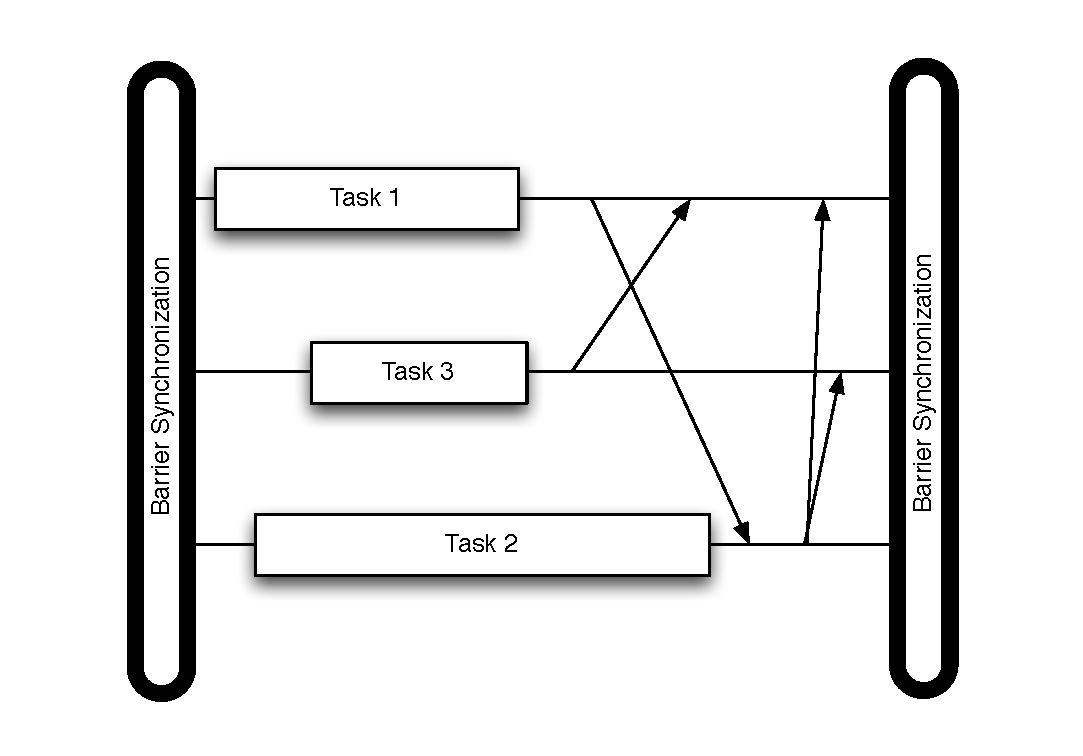
\includegraphics[width=0.5\linewidth]{img/BSP}
		%\vspace{-0.4cm}
		\caption{Un superstep dans le modèle BSP}\label{fig:Superstep}
\end{figure}

Une première implémentation du paradigme FIIT a vu le jour avec la plate-forme CONFIIT (Computation Over Network for FIIT) \cite{FKF03,Flauzac10}. CONFIIT a été développé en tant que middleware pour le calcul distribué, en s'appuyant sur un anneau logique (overlay) géré par le middleware et des échanges XML-RPC entre les n{\oe}uds. À la suite de sa version initiale, CONFIIT a été fortement modifié entre 2004 et 2006, avec l'addition de différents modes de calcul (distribué, centralisé), isolation (\textit{sandboxing}), observateurs extérieurs, etc. Ce développement a été fait notamment dans le cadre d'un projet supporté par l'agence ANVAR dans le but de créer une \textit{startup} dans le domaine du calcul distribué.
CONFIIT a été utilisé comme plate-forme de calcul pour plusieurs travaux, notamment lors de la résolution parallèle des instances L(2,23) et L(2,24) du problème de Langford \cite{JK04}.

Lors du démarrage du projet STIC-AmSud PER-MARE, nous avons voulu utiliser CONFIIT comme plate-forme pour l'exécution d'applications \textit{MapReduce}, mais nous avons rencontré plusieurs difficultés qui n'ont pas permis l'utilisation de CONFIIT pour la suite du projet. En effet, nous avons trouvé une faille dans la conception de l'anneau logique qui empêchait l'utilisation de CONFIIT pour les applications de type \textit{big data} : l'anneau était utilisé autant pour le passage des messages de service que pour la diffusion des données associées aux tâches. La transmission de masses de données plus importantes que quelques kilo-octets (ce qui était le cas avec Langford) occasionnait la congestion de l'anneau logique et empêchait la synchronisation des n{\oe}uds, causant ainsi leur déconnexion.

Après plusieurs tentatives, nous avons pris la décision de développer une nouvelle plate-forme, plus à jour et disposant de ressources capables de supporter aussi les applications de type \textit{big data}. Cette nouvelle implémentation, appelée CloudFIT, sera décrite dans les sections suivantes. 


\subsection{Spécification des besoins}

La décision d'implémenter une nouvelle plate-forme capable de supporter le paradigme FIIT (et ses variantes) dans un univers d'applications allant du calcul combinatoire au \textit{big data} a été suivie d'une liste d'exigences visant la généricité et la maintenance de la plate-forme :

\begin{description}
	\item [R1] CloudFIT doit être indépendant de l'overlay P2P. Ce choix rend possible le test de différents overlays P2P, afin de mieux s'adapter aux environnements et besoins des applications ;
	\item [R2] CloudFIT doit être modulable afin de supporter la composition et l'ajout de nouveaux modules, grâce à des interfaces et services bien définis. De plus, ceci doit permettre à l'utilisateur de composer "sa" pile logicielle sans avoir à modifier le code source, par exemple grâce à un fichier de configuration externe ;
	\item [R3] CloudFIT doit supporter le déploiement d'applications à la volée. Un utilisateur doit pouvoir soumettre ses propres classes applicatives à CloudFIT, qui les intégrera à la file d'exécution et les déploiera aux différents n{\oe}uds du réseau.
\end{description} 


L'objectif [R1] vient directement de l'expérience avec CONFIIT, où une dépendance trop forte par rapport au middleware P2P pourrait gêner l'évolution de la plate-forme. Comme les réseaux pervasifs présentent des grandes variations de performance et capacité, les couches les plus proches du réseau doivent pouvoir s'adapter à ces contraintes, comme par exemple l'impossibilité d'effectuer des diffusions, la présence de proxies et de passerelles NAT, voir même le support à des communications par mémoire partagée si l'environnement le supporte. Le respect à cet objectif a été très utile car l'overlay P2P initialement retenu (FreePastry\footnote{\url{http://www.freepastry.org/}}) s'est plus tard révélé peu performant et on a pu facilement migrer vers un nouvel overlay, TomP2P\footnote{\url{http://tomp2p.net}}. 

La règle [R2] est autant une prérogative visant l'évolution et la maintenance de la plate-forme qu'une manière de rendre plus simple l'expérimentation avec CloudFIT. De plus, le fait de reposer sur des interfaces permet une moindre dépendance entre les modules, demandant peu ou aucune modification de code en cas de remplacement d'un composant. 

Finalement, l'exigence [R3] garantit la scalabilité de la solution. En effet, il serait inconcevable d'avoir à distribuer l'application aux n{\oe}uds de calcul avant de lancer une application, comme c'était le cas avec CONFIIT. C'est bien le rôle de la plate-forme d'effectuer ce déploiement et d'assurer le lancement des applications selon des appels bien définis dans l'interface applicative. 

\subsection{Architecture}

L'architecture de CloudFIT a été conçue selon les objectifs cités précédemment. Afin de renforcer la modularité de la plate-forme, nous l'avons conçue sous la forme d'une pile logicielle, inspirée des modèles réseau TCP/IP et OSI. Ainsi, nous avons défini quatre couches représentant les différentes fonctionnalités de la plate-forme : \textbf{Network}, \textbf{Protocol}, \textbf{Service} et \textbf{Application}.

\begin{figure}
	\centering
		\includegraphics[width=0.65\linewidth]{img/CloudFITstack}
		\caption{Représentation simplifiée de la pile logicielle CloudFIT}\label{fig:cloudFitStack}
\end{figure}

Malgré son nom, la couche \textbf{Network} est responsable pour toute interaction avec les systèmes tiers sur lesquels CloudFIT s'appuie (overlay P2P, système  d'exploitation, systèmes de stockage). Par exemple, la classe \texttt{Network Adapter} exécute les opérations élémentaires d'encapsulation et décapsulation des messages, grâce à des primitives conçues selon les capacités des overlays P2P subjacents (\textit{send}, \textit{sendAll}, \textit{receive}, etc.). Le même principe s'applique à la classe \texttt{Storage Adapter}, où des primitives comme \textit{read}, \textit{write}, \textit{delete}, \textit{lookup} font l'interface avec les différentes solutions de stockage possibles (fichiers locaux, DHTs, bases de données, stockage sur le cloud). On y trouve finalement le \texttt{Context Collector}, déjà présenté dans le chapitre précédent en Section \ref{sec:gestionnairecontexte} et qui a été intégré à CloudFIT aussi.

La couche \textbf{Protocol} est responsable notamment par la gestion des messages et les ressources de calcul. Ainsi, le module \texttt{Core-ORB} (nommé ainsi car son rôle est comparable à celui d'un \textit{Object Request Broker}) stocke les messages reçus de la couche Network et délivre ces messages aux services adéquats de la couche supérieure. Grâce à un mécanisme \textit{publish-subscriber}, différents services peuvent s'enregistrer auprès le \texttt{Core-ORB}, obtenant ainsi un identifiant unique utilisé pour la réception des messages mais aussi pour des éventuelles communications entre les services dans le même n{\oe}ud. 

Le \texttt{Ressource Manager}, de son côté, puise dans les informations extraites par le collecteur de contexte pour vérifier si les ressources présentes dans la machine sont compatibles avec les besoins des applications. Ces besoins sont des propriétés fonctionnelles (mémoire disponible, espace disque, etc.) renseignées par l'application lors de sa soumission. Le \texttt{Ressource Manager} est aussi responsable pour la gestion du pool de \texttt{Workers}, qui sont alloués aux applications selon les demandes faites par les ordonnanceurs de tâches. 

La couche \textbf{Service}  contient les services nécessaires à l'exécution des applications distribuées. À cette couche appartient notamment la classe \texttt{Community}, une abstraction d'un groupe de machines qui gère le déploiement des applications et la gestion des événements liés aux n{\oe}uds (entrée, sortie, retransmission de messages, etc.). Chaque communauté est associée à un \texttt{JobScheduler}, qui gère la file d'applications soumises (jobs) et choisit lesquelles peuvent être lancées sur la machine, en croisant les contraintes des applications et les informations du \texttt{RessourceManager}.  Il faut remarquer que plusieurs communautés peuvent coexister sur un n{\oe}ud et dans le réseau, permettant ainsi la création de sous-ensembles de n{\oe}uds et le déploiement d'applications selon différents critères.

 D'autres services de cette couche incluent des interfaces de soumission ou de visualisation des résultats. Ces services sont notamment utiles dans l'interaction avec des dispositifs IoT qui n'ont pas la possibilité d'exécuter une instance de CloudFIT, comme par exemple les micro-contrôleurs Arduino. Dans ce cas, il suffit d'offrir un accès à un n{\oe}ud CloudFIT grâce à une interface REST ou JSON, comme suggère la Figure \ref{fig:cloudFitStackIoT}. Ces interfaces peuvent être utilisées autant pour le simple stockage de données que pour le déclenchement d'applications.

\begin{figure}
	\centering
		\includegraphics[width=0.65\linewidth]{img/CloudFITstack-IoT}
		\caption{Exemple d'interface IoT pour l'interaction avec CloudFIT}\label{fig:cloudFitStackIoT}
\end{figure}


Finalement, la couche \textbf{Application} contient les éléments nécessaires à l'exécution de l'application fournie par l'utilisateur. Cette couche spécifie l'interface applicative qui doit être implémentée par l'application utilisateur afin d'être exécutée par CloudFIT. L'interface applicative est assez simple et intuitive, suivant les principes du paradigme FIIT. Ainsi, le développeur n'a besoin que d'écrire les méthodes suivantes :
\begin{description}
	\item [numberOfBlocks()] méthode qui retourne le nombre de tâches à lancer. Cette méthode est appelée pendant la configuration du \texttt{TaskScheduler} ;
	\item [executeBlock(taskID, required{[]}) ] méthode qui démarre l'exécution proprement dite de la tâche, c'est le point d'accroche pour les \texttt{Workers}. Le \textit{taskID} permet à la tâche de personnaliser son exécution, et l'élément \textit{required[taskID]} indique les éventuelles dépendances de cette tâche. Ce paramètre est aussi utilisé par le \texttt{TaskScheduler} pour gérer l'ordre d'exécution afin de respecter les dépendances ;
	\item [finalizeApplication()] méthode optionnelle qui est exécutée par le \texttt{TaskScheduler} une fois que l'ensemble de tâches est terminé. Cette méthode permet l'agrégation des résultats, à l'instar d'une phase Reduce dans le paradigme \textit{MapReduce}.
\end{description}

On y trouve aussi la classe\texttt{ TaskScheduler}, un ordonnanceur associé à chaque job et responsable par la gestion des tâches et l'interaction avec le \texttt{RessourceManager} afin d'obtenir des \texttt{Workers} pour exécuter ces tâches. L'interaction entre le \texttt{TaskScheduler}, l'application et les autres éléments de la couche Service est présentée de manière simplifiée en Figure \ref{Figure:applayer}. 

\begin{figure}
	\centering
		\includegraphics[width=0.65\linewidth]{img/CloudFITstack-app}
		\caption{Diagramme simplifié de l'interaction entre les éléments lors du lancement d'un job et de ses tâches}\label{Figure:applayer}
\end{figure}

Il faut noter que la classe \texttt{TaskScheduler} est extensible et personnalisable. Par défaut CloudFIT fournit un ordonnanceur simple, mais celui-ci peut être remplacé par des ordonnanceurs plus élaborés. L'ordonnanceur par défaut fait juste une redistribution aléatoire des tâches, une technique simple qui réduit le risque de travail en doublon entre les n{\oe}uds. Parmi les exemples d'ordonnanceurs plus élabores on peut citer ceux qui prennent en charge les dépendances entre les tâches (dans le cas d'une application DAG) ou qui utilisent des éléments de contexte comme par exemple la localisation d'un n{\oe}ud pour minimiser le temps d'accès aux données. 




\subsection{Communication\label{subsec:commCloudFIT}}

La section précédente illustrait la structuration et l'interaction des modules dans une machine. Cependant, une plate-forme de calcul distribué se doit de garantir les échanges entre les différents n{\oe}uds sur le réseau. Dans le cas de CloudFIT, le choix d'utiliser un overlay P2P tiers simplifie les opérations de découverte de pairs, la gestion du réseau (entrées, sorties), routage des messages, etc. Nous pouvons ainsi nous concentrer sur la communication intrinsèque à la plate-forme, comme par exemple le déploiement des applications, le suivi de la progression de l'exécution et la distribution/récupération des résultats. 

Tout démarre par la soumission d'un job, effectué directement par un n{\oe}ud déjà connecté au réseau ou grâce à une interface de soumission. Cette soumission contient le code applicatif, le nom de la Community cible, ainsi qu'une liste de propriétés nécessaires à la bonne exécution du job. Ce message est envoyé à travers le réseau, grâce aux mécanismes de diffusion de l'overlay P2P ou, le cas échéant, grâce à une diffusion de type \textit{best-effort}.

Comme spécifie l'objectif [R3], nous devons garantir qu'une application sera déployée par la plate-forme elle-même car il serait très contraignant pour l'utilisateur de placer l'application sur chaque n{\oe}ud. Afin de répondre à ce besoin, nous avons choisi d'utiliser le stockage DHT habituellement associé aux overlays P2P. En effet, le DHT offre à tous les n{\oe}uds de l'overlay un accès réseau à des objets et fichiers, du moment où ces n{\oe}uds connaissent la clé des ressources. Ainsi, la soumission d'un job comprend l'enregistrement d'un fichier \textit{jar} contenant le code applicatif et la clé DHT de cette ressource. Au moment du lancement du job, le \texttt{JobScheduler} récupère ce fichier et extrait ses classes, qui seront chargés grâce à un \textit{classloader}. 

Le stockage DHT peut aussi être utilisé pour la mise à disposition de données d'entrée pour les applications, comme par exemple dans le cas d'une application \textit{big data}. Ceci n'est pas obligatoire, vu que les applications ont aussi la possibilité d'obtenir les données via des ressources extérieurs (URLs, stockage cloud, bases de données).

Lorsqu'un job démarre sur une machine, son statut passe de \textit{NEW} à \textit{STARTED}. À ce moment le \texttt{TaskScheduler} associé à ce job est démarré, et les tâches peuvent être lancées. Celles-ci ont 5 états possibles : \textit{NEW}, \textit{STARTED}, \textit{STARTED\_DISTANT}, \textit{COMPLETED} et \textit{DISTANT}. 

Lorsqu'une tâche est lancée, un message est envoyé aux n{\oe}uds de la \texttt{Community} indiquant le ID du job et de la tâche. Ceci permet aux \texttt{TaskScheduler} des autres n{\oe}uds de savoir cette tâche est traitée par une autre machine et ainsi réduire le travail en doublon : ces tâches "distantes" sont marquées comme \textit{STARTED\_DISTANT} et sont placées à la fin de la file d'exécution. Une tâche marquée ainsi ne sera exécutée que lorsque toutes les tâches \textit{NEW} ont été épuisées et, bien sûr, si aucun message n'est venu indiquer que la tâche a été complétée. En effet, le \texttt{TaskScheduler} envoie un deuxième message à la fin de l'exécution d'une tâche, indiquant le changement de son statut à \textit{COMPLETED} et aussi indiquant le résultat de son calcul (ou bien les coordonnées pour retrouver ce résultat, si stockés dans la DHT ou dans une ressource externe).

Si un n{\oe}ud finit l'exécution de toutes ses tâches \textit{NEW}, il peut démarrer l'exécution de tâches spéculatives parmi celles marquées \textit{STARTED\_DISTANT}. Ce mécanisme garantit la terminaison de toutes les tâches (si le n{\oe}ud original est défaillant) et permet même d'accélérer la terminaison du calcul si le n{\oe}ud original est trop lent.

En plus de mettre à jour les autres n{\oe}uds, ces échanges de messages ont aussi le rôle de mettre au courant un nouveau n{\oe}ud qui rejoint le réseau. En voyant passer des messages de type "task completed", les n{\oe}uds peuvent demander à un voisin de les transmettre le message avec la description du job. Son \texttt{TaskManager} va donc procéder à la récupération des tâches \textit{DISTANT} grâce à des requêtes spécifiques. Ce mécanisme permet ainsi de garantir l'intégration des n{\oe}uds dans un environnement volatile et d'assurer la pérennité des résultats. En effet, il suffit qu'une machine subsiste dans le réseau pour que les résultats restent accessibles.

À la fin de l'exécution de toutes les tâches, les \texttt{TaskManager} récupèrent l'ensemble des résultats locaux ou distants et le statut du job devient \textit{COMPLETED}. Ce job reste à la disposition de toute application ou n{\oe}ud qui souhaite récupérer ses résultats.


\section{Calcul Multi-échelle et le \textit{Fog Computing}}

Comme indiqué précédemment, la plupart des travaux sur le \textit{edge/fog computing} ont la tendance à faire une distinction entre l'utilisateur final (ou les périphériques finaux) et les dispositifs qui se trouvent à la frontière de l'Internet/\textit{cloud}. Dans de telles approches, les appareils IoT sont des simples clients des services déployés dans un voisinage proche, ce qui est d'une certaine manière contraire aux principes du \textit{fog computing}, où tous les dispositifs peuvent contribuer au calcul des tâches selon leurs propres capacités et ressources disponibles. 

Cependant, les réseaux P2P les plus connus organisent les n{\oe}uds indistinctement de leur emplacement réel, ce qui empêche l'établissement de services de proximité à faible latence. Pour contourner ces inconvénients, nous considérons que le réseau P2P de CloudFIT doit être enrichi par l'utilisation du concept du calcul multi-échelle \cite{Rottenberg2012,Rottenberg2014}  associé à des techniques de \textit{clustering}. En effet, le regroupement des ressources sous la forme de \textit{clusters} est une manière efficace pour organiser les couches de calcul multi-échelle et ainsi fournir une base de coordination pour le déploiement efficace des services.

\subsection{Clustering}

Plusieurs approches de clustering sont proposées dans la littérature \cite{Johnen2011} et utilisées, par exemple, pour  le routage des informations dans les réseaux de capteur sans fil. La plupart des algorithmes de clustering utilisent des paramètres simples comme la densité du réseau environnant, choisissant un \textit{cluster-head} en fonction de leurs identités uniques (ID). Malheureusement, ces métriques sont insuffisantes pour assurer le clustering dans un scénario hétérogène, vu qu'elles ne permettent pas d'exprimer les besoins du calcul multi-échelle. 

Dans notre cas, nous devons permettre le regroupement des n{\oe}uds selon différentes stratégies de manière à co-localiser les données et les ressources nécessaires pour les services de proximité mais aussi faire des ponts pour relier les dispositifs proches et ceux plus éloignés, même jusqu'au cloud. Ainsi, afin de s'adapter à l'hétérogénéité des environnements pervasifs et l'IoT, les métriques de clustering doivent inclure des informations de contexte telles que la proximité, les capacités informatiques et de stockage des appareils, la fiabilité et même le niveau d'autorisation/confiance des n{\oe}uds collaborateurs.
 
Dans le cas de CloudFIT, ce clustering peut être mis en {\oe}uvre grâce aux \textit{communautés}, en créant des sous-ensembles de n{\oe}uds qui peuvent être adressés séparément et donc utilisés pour répartir/cloisonner les opérations. Bien entendu, un n{\oe}ud peut appartenir à plusieurs communautés, permettant à des données et des tâches de circuler entre les différentes couches multi-échelle, comme illustrée en Figure \ref{fig:antennes}. Cette organisation à plusieurs niveaux en fonction du contexte des ressources disponibles permettrait de mieux coordonner la communication entre ces ressources et d'ainsi mieux gérer la variabilité d'échelle de ces environnements. 

 
 \begin{figure}[!ht]
 	%\renewcommand{\figurename}{Figura}
 	\centering
 	%\vspace{-0.3cm}
 	\includegraphics[width=0.6\linewidth]{img/antennes2.pdf}
 	%\vspace{-0.2cm}
 	\caption{Exemple de communautés interconnectées dans une plate-forme multi-échelle}
 	\label{fig:antennes}
 	%\vspace{-0.5cm}
 \end{figure}

\subsection{Optimisations pour le \textit{big data}}
%
Dans le cadre du traitement de données issus des dispositifs de l'IoT, un autre facteur à prendre en compte est celui de la performance liée à l'accès et à la gestion des données. En effet, la plupart des opérations impliquent la collecte, la transformation et l'analyse des données, et les plates-formes telles que Apache Hadoop se sont illustrées par leur capacité d'optimiser l'accès aux données en plaçant les tâches préférentiellement là où les données sont présentes (grâce au concept de la \textit{data locality}). 

Dans le passé \cite{Steffenel2015Roma} nous avons déjà mené des expérimentations avec CloudFIT démontrant que des performances similaires ou supérieures à celles de Apache Hadoop pourraient être atteintes avec un système P2P, comme illustré en Figure \ref{fig:Hadoop}. Bien que ces résultats aient été positifs, nous avons observé deux points qui pourraient être encore améliorés : la surcharge de gestion des données sur un n{\oe}ud et la prise en charge de la \textit{data locality}. 

\begin{figure}[!ht]
	%\renewcommand{\figurename}{Figura}
	\centering
	%\vspace{-0.3cm}
	\includegraphics[width=0.65\linewidth]{img/CloudFIT-mesures.pdf}
	%\vspace{-0.2cm}
	\caption{Comparaison des temps d'exécution de WordCount avec CloudFIT et Hadoop}
	\label{fig:Hadoop}
	%\vspace{-0.2cm}
\end{figure}

Dans le premier cas, nous avons constaté un fort écart de performances d'accès aux données lorsque nous déployons CloudFIT  dans un environnement hétérogène. Ces écarts de performance sont en effet une combinaison de la vitesse d'accès aux données et de la surcharge de gestion des systèmes de stockage (voir aussi les limitations physiques de stockage), et affectent notamment les dispositifs de faible capacité. Ainsi, par exemple, un Raspberry Pi est fortement pénalisé par la vitesse et la capacité de stockage de sa carte SD, malgré une capacité de calcul suffisante (notamment en utilisant tous ses c{\oe}urs de calcul).  

Afin de contourner cette limitation, nous avons modifié la couche de stockage de manière à ce que les n{\oe}uds puissent choisir d'agir seulement en tant que clients distants. Ces n{\oe}uds peuvent donc interroger le service de stockage DHT via le réseau mais ils ne sont plus obligés à gérer le stockage, réduisant leur surcharge et aussi leur utilisation du disque.

Pour ce qui est de la prise en charge de la \textit{data-locality}, cela est un problème plus général qui affecte la plupart des architectures de stockage P2P. En effet, les API de stockage P2P sont souvent basés sur les tables de hachage distribuées (DHT). Ces DHTs sont conçues de manière à répartir les données sur le réseau et les répliquer lorsque cela est possible, notamment afin d'éviter la perte de données en cas de désabonnement (\textit{churn}). Un inconvénient de cette procédure est qu'on observe une perte d'information concernant la localisation des données \cite{Wu2005}, rendant difficile l'optimisation des transferts réseau. Nous avons donc développé deux mécanismes distincts visant à contourner cette limitation. 

La première approche que nous avons développée peut facilement être mise à l'{\oe}uvre si on un accès à la bibliothèque DHT. Cette stratégie consiste à instruire l'ordonnanceur de tâches (\textit{TaskScheduler}) à vérifier préalablement quelles tâches seraient favorisées par la présence des données dans son cache DHT local. Même si c'est une opération de bas niveau, la plupart des DHT P2P offrent la possibilité d'effectuer un \textit{lookup} pour savoir si la ressource requise se trouve déjà dans le cache local ou s'il faut la chercher sur le réseau. En donnant la priorité aux tâches qui peuvent travailler avec des données locales, on peut espérer augmenter la performance globale de l'exécution.

Toutefois, il n'est pas toujours possible d'avoir des données en local dans un overlay P2P. En effet, dans une DHT les n{\oe}uds responsables par le stockage et indexation des ressources sont définis par la clé de hachage de la ressource. La Figure \ref{fig:pastry} illustre le cas du routage d'un message dans l'overlay Pastry \cite{Pastry01, Castro2002}, mais le même exemple peut être utilisé pour la localisation des ressources dans la DHT PAST \cite{Rowstron2001b} car dans ce système les clés des ressources et les clés des n{\oe}uds se superposent. Finalement, même avec de la réplication, il y a le risque que dans un grand réseau les ressources ne se trouvent sur aucun des n{\oe}uds de calcul. Ceci nous amène à l'élaboration d'une stratégie pour renforcer la proximité des données, grâce à un calcul personnalisé de la clé de localisation des ressources. 


\begin{figure}[!ht]
	%\renewcommand{\figurename}{Figura}
	\centering
	%\vspace{-0.3cm}
	\includegraphics[width=0.4\linewidth]{img/AnneauPastry.pdf}
	%\vspace{-0.2cm}
	\caption{Exemple de routage d'un message dans l'overlay Pastry \cite{Castro2002}}
	\label{fig:pastry}
	%\vspace{-0.2cm}
\end{figure}


Cette technique a été élaborée sur la base des spécificités de la DHT de TomP2P, et donc ne peut pas être facilement généralisée. Contrairement à la plupart des systèmes de P2P qui ont seulement une clé de hachage, TomP2P identifie les ressources par quatre clés différentes $\{k_l,k_d,k_c,k_v\}$, selon la hiérarchie suivante : 
\begin{itemize}
	\item \textit{$k_l$} - clé de localisation, utilisée pour la localisation d'une ressource dans la DHT ;
	\item \textit{$k_d$} - clé de domaine, fonctionne comme une clé d'authentification, permet la séparation des données ;
	\item \textit{$k_c$} - clé de contenu, permet d'identifier une ressource. Par défaut celle-ci est identique à la clé de localisation ;
	\item \textit{$k_v$} - clé de version, permet la gestion de versions multiples d'une ressource.
\end{itemize} 

La clé de localisation est celle qui s'approche le plus des clés DHT traditionnelles, ayant par fonction l'association d'une ressource (copie primaire ou index) au n{\oe}ud avec l'ID le plus proche. Sans aucune instruction supplémentaire, la clé de localisation et la clé de contenu sont les mêmes, mais peuvent être différentes par exemple pour résoudre les cas de collision de clés (deux ressources générant la même clé de localisation).

La clé de domaine est liée à un mécanisme d'authentification simple de TomP2P, son but étant de renforcer le cloisonnement des données des différents clients (cette authentification peut être renforcée par l'utilisation de la cryptographie afin de garantir une véritable confidentialité). Dans le cas de CloudFIT, la clé de domaine est utilisée comme un \textit{namespace} pour la séparation des données de différents communautés ou jobs de calcul. 

Finalement, la clé de version permet la coexistence de différentes versions d'une ressource, ce qui permet une meilleure gestion des données "mutables", avec par exemple un accès à l'historique des modifications ou l'écriture en parallèle d'une ressource par plusieurs n{\oe}uds. Cette clé de version est utilisée dans les nouvelles versions de l'application \textit{MapReduce} développée sur CloudFIT.

Ainsi, afin de renforcer la \textit{data locality}, nous avons travaillé sur le découplage entre la clé de localisation et la clé de contenu grâce à une double fonction de hachage. Dans un premier moment, la clé de contenu est obtenue avec une méthode de hachage classique. Ensuite, la clé de localisation est calculée en faisant une association limitée aux ID des n{\oe}uds d'une communauté. La Figure \ref{fig:hash} montre l'exemple de cette cartographie en calculant la clé de localisation d'une ressource $r_3$ par rapport à une communauté $Comm_1$.

\begin{figure}[!ht]
	%\renewcommand{\figurename}{Figura}
	\centering
	%\vspace{-0.3cm}
	\includegraphics[width=0.5\linewidth]{img/hashing.pdf}
	%\vspace{-0.2cm}
	\caption{Cartographie des ressources renforçant la data-locality}
	\label{fig:hash}
	%\vspace{-0.2cm}
\end{figure}

Comme la clé de localisation se trouvera parmi les n{\oe}uds de la communauté, on augmente la probabilité de trouver la copie primaire dans les n{\}oe}uds concernés. De plus, cette stratégie n'empêche pas la réplication des données sur d'autres n{\oe}uds, garantissant la persistance des données en cas de défaillances. Cette approche est aussi tolérante aux variations du nombre de membres de la communauté : en cas de disparition d'un n{\oe}ud, c'est une réplique qui prend le relais ; en cas d'un nouveau membre, celui-ci sera intégré à la fonction de hachage normalement.   

\section{Exemples d'Utilisation de CloudFIT}

En tant que plate-forme expérimentale pour le calcul distribué et le \textit{fog computing}, CloudFIT est en constante évolution. Cela n'empêche pas son utilisation comme plate-forme de calcul dans certains de nos projets, notamment ceux dont l'objectif est d'utiliser des réseaux avec des éléments volatiles ou avec des ressources hétérogènes. Le premier exemple ci-dessous illustre une utilisation "recherche" pour le projet STIC-AmSud PER-MARE, dans le but d'évaluer le comportement de CloudFIT en tant que plate-forme \textit{MapReduce} pour les environnements pervasifs. Le deuxième exemple démontre une utilisation "production", où CloudFIT a été utilisé pour exécuter un workflow destiné aux sciences de l'atmosphère. Ce dernier travail a servi de base  pour la proposition du projet de collaboration CAPES-Cofecub MESO. 


\subsection{L'application WordCount}

Le projet STIC-AmSud PER-MARE (\textit{Adaptive Deployment of MapReduce-based Applications over Pervasive and Desktop Grid Infrastructures}) avait pour but le développement de stratégies pour le déploiement d'applications \textit{MapReduce} sur des environnements pervasifs. Si l'un des volets du projet a été celui d'adapter Apache Hadoop (voir la Section \ref{sec:Guilherme}), l'autre volet consistait à utiliser CloudFIT en tant que plate-forme de calcul distribuée. Si dans l'article présenté à CLIoT 2015 \cite{Steffenel15Taormina} nous nous sommes concentrés sur la performance de CloudFIT (voir aussi la Figure \ref{fig:Hadoop}), le travail présenté à CN4IoT \cite{Steffenel2015Roma} analysait l'exécution de CloudFIT par rapport à la volatilité et l'hétérogénéité des ressources.

\subsubsection{Impact de la volatilité}

Cette première expérience illustre le déploiement d'une application \textit{MapReduce} simple (\texttt{WordCount}) sur un corpus de textes faisant 1 GB de données et réparti en blocs uniformes de 64 MB. Cette répartition vise à reproduire le comportement de Hadoop, qui lui aussi traite les données par blocs de 64 MB.  Aussi afin de rendre la visualisation des expériences plus simple, les n{\oe}uds sont identiques et ont été explicitement limités à une seule exécution simultanée (un seul \texttt{Worker}). 

Dans un premier moment et afin d'avoir un barème de comparaison, la Figure \ref{fig:regular} présente le diagramme de Gantt pour une exécution sans incidents.
Nous pouvons avoir un aperçu du mécanisme d'ordonnancement distribué par défaut de CloudFIT, déjà discuté en Section \ref{subsec:commCloudFIT}. En effet, lorsque la liste de tâches est reçue par le TaskScheduler, celle-ci est réordonnée de manière aléatoire. L'ordonnanceur choisit ainsi la première tâche disponible (marquée "\textit{NEW}") et avertit les autres n{\oe}uds que cette tâche est en exécution. De manière similaire, à la fin de son exécution son statut est diffusé pour annoncer la fin de la tâche. Si toutes les tâches "\textit{NEW}" ont déjà été prises, un n{\oe}ud peut lancer des tâches spéculatives parmi celles marquées "\textit{STARTED\_DISTANT}". 

Plus spécifiquement, nous pouvons observer le déploiement des tâches \textit{map} (lesquelles ont des temps d'exécution variable selon le nombre de mots dans les documents), plus une tâche \textit{reduce} qui s'exécute à la fin. Bien que l'exemple \texttt{WordCount} ne contienne qu'une tâche Reduce, celle-ci se trouve exécutée par tous les n{\oe}uds car si le premier n{\oe}ud a marqué la tâche comme "\textit{STARTED}" et prévient les autres, ceux-ci n'ont rien de plus dans leur file d'exécution et lancent le Reduce en tant que tâche spéculative. Ceci n'a aucun impact sur le résultat final de l'application car les n{\oe}uds vérifient la présence d'un fichier de sortie avant de l'écrire sur la DHT, empêchant tout écrasement ou corruption. 

\begin{figure}
	\centering
		\includegraphics[width=1\linewidth]{img/regular2}
		\caption{Exécution de WordCount sur un cluster uniforme (1 GB de données en blocs de 64MB)}\label{fig:regular}
\end{figure}




Grâce à ces échanges, il est aussi possible de compléter les tâches initiées par les n{\oe}uds en défaillance ou mettre au courant un n{\oe}ud qui vient de rejoindre une communauté CloudFIT. La Figure \ref{fig:1out} représente ainsi une situation où un n{\oe}ud tombe en panne, avec la subséquente reprise des tâches par les autres n{\oe}uds. La Figure \ref{fig:reprise} va au-delà de cette situation en rajoutant un nouveau n{\oe}ud, qui récupère l'état actuel des tâches et peut ainsi contribuer avec l'effort de calcul.
\begin{figure}
	\centering
		\includegraphics[width=1\linewidth]{img/1out2}
		\caption{Exécution de WordCount lorsqu'un n{\oe}ud disparaît (1 GB de données en blocs de 64MB)}\label{fig:1out}
\end{figure}

\begin{figure}
	\centering
		\includegraphics[width=1\linewidth]{img/reprise2}
		\caption{Exécution de Wordcount lorsqu'un n{\oe}ud rejoint la communauté après la défaillance d'un autre n{\oe}ud (1 GB de données en blocs de 64MB)}\label{fig:reprise}
\end{figure}


\subsubsection{Impact de l'hétérogénéité}

Cette deuxième expérience vise l'observation de CloudFIT dans un environnement hétérogène. Pour cela, nous avons interconnecté quatre n{\oe}uds avec des spécifications assez différentes (cf. le Tableau \ref{Table:laptops}). Comme dans l'expérience précédente, nous limitons le nombre de c{\oe}urs (\texttt{Workers}) sur les machines pour rendre la visualisation plus simple.

\begin{table}
	\begin{center}
		\begin{tabular}{|c|c|c|c|c|c|c|}
			\hline
			Type de N{\oe}ud & Processeur & GHz &  Mémoire & OS\\
			\hline
			\hline
			MacBook Air & Intel Core i7-4650U & 1.7   & 8 GB & MacOS 10.10.5 \\
			Lenovo U110 & Intel Core2 Duo L7500 & 1.6   & 4 GB & Ubuntu Linux 15.4 \\
			Raspberry Pi 2 & ARM Cortex-A7 & 0.9  & 1 GB & Raspbian Linux Wheezy\\
			VM Virtualbox & Intel Core i7* & 2.2*  &  1 GB & Debian Linux 8.2 \\
			\hline
			\multicolumn{5}{l}{* ces valeurs sont celles vues par la machine virtuelle}
		\end{tabular}
	\end{center}
	\caption{\label{Table:laptops}Spécification des n{\oe}uds du cluster pervasif}
\end{table} 

Nous avons aussi modifié les paramètres de l'expérience afin d'exécuter le WordCount sur 512MB de données divisées en petits blocs de 2MB seulement ; nous pensons que cette configuration est plus proche de celle rencontrée lors de la transmission de données par les dispositifs IoT. La multiplication de tâches avec un coût individuel plus réduit rend aussi possible la participation des n{\oe}uds avec moins de puissance de calcul.  La Figure \ref{fig:hetero} affiche le diagramme de Gantt pour une exécution de ce scénario. 

\begin{figure}
	\centering
		\includegraphics[width=1\linewidth]{img/hetero2}
		\caption{Exécution de Wordcount dans un cluster hétérogène (512MB en blocs de 2MB)}\label{fig:hetero}
\end{figure}

Alors que la répartition des tâches entre les notebooks et la machine virtuelle ne présentent pas une différence significative, le Raspberry Pi, sans surprise, n'arrive pas à exécuter les tâches aussi vite que les autres n{\oe}uds (voir la longueur des tâches dans la première partie de l'exécution). De plus, ce n{\oe}ud est tellement surchargé qu'il perd plusieurs messages de mise à jour et ne détecte pas la fin de la phase \textit{map}. Comme résultat, il essaye vainement d'exécuter toutes les tâches juste pour se rendre compte que leur résultat est déjà dans la DHT, la raison pour la petite durée des tâches vers la fin (cette vérification préalable était prévue pour éviter le travail en doublon et les risques de corruption des données). 

Au lieu de freiner notre intérêt par les dispositifs de faible puissance, ces résultats nous incitent à vouloir comprendre les raisons de ces problèmes. En effet, les dispositifs de faible puissance tels que les Raspberry Pi n'ont pas seulement des processeurs moins rapides mais aussi des limitations sur la taille et la vitesse d'accès à la mémoire et au stockage (quelques centaines de MB de RAM, des mémoires SD à la place des disques durs, etc.). Dans ces dispositifs, les tâches de gestion de l'overlay P2P et de la DHT (par exemple, la réplication des données) peuvent occuper une partie importante de leurs ressources et finir par interférer avec le traitement des messages échangé via l'overlay.  Ces résultats ont motivé la mise en place des stratégies de collecte de contexte pour un meilleur ordonnancement et aussi les méthodes d'optimisation du stockage que nous avons détaillé dans la section précédente. 

\subsection{Détection d'Événements Secondaires de la Couche d'Ozone}

La découverte du trou d'Ozone de l'Antarctique \cite{Farman1985} a galvanisé l'intérêt de la communauté scientifique et depuis ce moment plusieurs études ont été menées dans le but de surveiller la variation de la densité de la couche d'Ozone sur les régions polaires \cite{Solomon1999}\cite{Salby2012}. La réduction de la couche d'Ozone peut aussi déclencher plusieurs événements sur des zones situées à des latitudes moyennes, soit à cause du mouvement de la bordure du vortex polaire sur ces régions  \cite{Kirchhoff1997}\cite{Marchand2005} ou bien à cause du transit de masses d'air pauvres en Ozone détachées du vortex polaire. Ce dernier cas est appelé "événements dus à l'influence du trou d'ozone Antarctique", ou plus simplement des Événements Secondaires de l'Ozone" (\textit{Ozone Secondary Events}  - OSE). 

Causés par la circulation de l'atmosphère, ces masses d'air continuent à se déplacer pendant 7 à 20 jours après leur séparation du vortex polaire et peuvent atteindre des latitudes plus élevées, occasionnant une réduction temporaire de la colonne totale d'Ozone (\textit{Total Column Ozone} - TCO) sur des zones qui sont souvent habitées \cite{Prather1990}\cite{Waugh1994}\cite{Manney1994}. Comme résultat, des niveaux élevés de radiation ultraviolet nocive (UVB et UVC) atteigne la surface \cite{Casiccia2008}, à un tel point qu'une réduction de 1\% de la colonne totale d'Ozone peut occasionner une augmentation de 1.2\% de la radiation UV mesurée sur le sud du Brésil \cite{Guarnieri2004}. Ces événements secondaires de l'Ozone sont régulièrement observés sur des zones peuplés en moyenne latitude, comme par exemple en Amérique du Sud \cite{Kirschhoff1996}\cite{Pinheiro2011}, en Afrique du Sud \cite{Semane2006}\cite{Sivakumar2007}, à la Nouvelle Zélande \cite{Brinksma1998} et aussi sur l'Île de la Réunion \cite{toihir2015}. 

%\begin{figure}
%	\centering
%	\includegraphics[width=0.75\linewidth]{img/22_10_13-c}
%	\vspace{-0.2cm}
%	\caption{OMI satellite image for 18 October 2013 (a) and the associated wind currents for (b) 19 and (c) 22 October 2013 at 620K}
%	\label{fig:event2013}
%	\vspace{-0.3cm}
%\end{figure}

Malgré une forte liaison avec la dynamique de la stratosphère, le nombre d'études visant la modélisation de la circulation dynamique de la couche d'Ozone sont encore très rares \cite{Marchand2005}. En effet, la plupart des modèles climatiques se limitent aux couches inférieures de l'atmosphère, notamment celles liées à aux prévisions météorologiques, et n'explorent pas les interactions avec les couches supérieures comme celle où se trouve la couche d'Ozone. Plus récemment, un modèle obtenu par Vaz Peres \cite{Peres2013} a permis une certaine compréhension de ces phénomènes. En se concentrant sur les données d'épisodes OSE déjà identifiés dans le passé, le modèle de Vaz Peres a permis la reproduction des événements observés. En partant de cette étude, notre but était d'utiliser des techniques du \textit{big data} et du \textit{data mining} afin de ramasser plus de données et extraire des modèles plus précis, permettant la prévision des occurrences de ces événements.

L'utilisation de techniques du \textit{big data} est essentiel car les données concernant la couche d'Ozone s'accumulent d'année en année. Par exemple, l'équipement TOMS/OMI placé dans les satellites de la NASA satellite produit plus d'1GB de données brutes par an. Juste les observations des satellites TOMS/OMI remontent à 1978 (ce qui fait presque 40 GB en ce moment), et à cela on peut rajouter d'autres sources de données satellites telles que les satellites de l'ESA mais aussi des observations effectuées au sol. 

\subsubsection{Identification des événements secondaires de l'Ozone avec CloudFIT\label{sec:development}}

Si dans un premier temps l'usage d'une plate-forme type cluster ou cloud pourrait être envisagée, notre attention s'est portée sur CloudFIT car celui-ci a l'avantage d'exploiter les ressources de calcul disponibles, sans obliger l'installation ou la maintenance d'un parc informatique dédié. En autre, le traitement des données et la détection des OSE varie selon la zone géographique couverte et selon le type d'analyse effectuée : la détection d'événements passés utilisée pour améliorer les modèles est assez simple, alors qu'une analyse plus poussée visant l'étude des corrélations entre les événements et les courants atmosphériques peut s'avérer bien plus demandeuse de ressources. L'utilisation de CloudFIT permet la création d'une plate-forme de calcul élastique.

Dans le cas précis de la détection des OSE, nous avons identifié quatre activités principales qui peuvent être transposées sur CloudFIT. Ces activités sont les suivantes : 
\begin{enumerate}
	\item \textbf{Pré-traitement des données} - transformation des données brutes OMI ;
	\item \textbf{Filtrage et agrégation} - sélection des données concernant une zone géographique et une période donnée, puis des opérations d'agrégation si nécessaire ;
	\item \textbf{Extraction des paramètres} - extraction des moyennes et écarts types pour une région et une période donnée ;
	\item \textbf{Détection des événements} - identification des valeurs anormales d'Ozone, génération d'alertes.
\end{enumerate}

Le pré-traitement des données est nécessaire car les données brutes fournis par l'équipement TOMS/OMI sont dans un format difficile à utiliser. Le filtrage permet de limiter la recherche sur une zone géographique et/ou sur une période d'étude, alors que l'agrégation permet l'obtention de données à une granularité différente de celle d'origine (utile notamment pour la corrélation avec d'autres types de données). En effet, la plupart des données TOMS/OMI ont une résolution d'1 dégrée, alors que d'autres sources de données ont parfois des cartographies plus détaillées (par exemple, avec 0.25 dégrée d'arc entre chaque mesure). Cette procédure sera détaillée dans la section suivante.

L'extraction des paramètres est la prochaine étape car la détection d'un OSE est liée à l'observation d'une chute anormale de la concentration de l'Ozone. Pour cela, il faut extraire des paramètres historiques tels que la moyenne et la variation (écart-type), et cela pour chaque coordonnée analysée. Cette procédure est aussi détaillée dans les sections suivantes. Finalement, la détection se fait en comparant la mesure d'un instant précis avec la série temporelle des journées précédentes. Si les valeurs sont inférieures à la variation normale de la période, alors on peut déclencher une procédure d'alerte, signalant aux autorités sanitaires un risque lié à la radiation UV qui menace la population.

Les trois premières activités sont des exemples d'opérations ETL (\textit{Extract, Transform, Load}) typiques du \textit{big data}. La dernière activité peut être considérée comme un algorithme de prise de décisions. Nous avons donc établi un workflow qui peut être transcrit comme un enchaînement de jobs CloudFIT, comme illustré en Figure \ref{fig:blocs}. Par conséquent, les quatre premiers jobs (Preprocess, Filtering, Time-series et Detection) peuvent même être exécutés sur des communautés CloudFIT différentes : des équipements entrée de gamme regroupés en Community C1 peuvent être utilisés pour pré-traiter et stocker les données des satellites et des spectre-photomètres Brewer ou Dobson installés au sol. 

Par la suite, les données peuvent donc être traitées pour la détection ou bien être utilisées pour des analyses plus poussées telles que la recherche de motifs récurrents ou la prévision d'événements futurs. Les activités telles que le filtrage et l'analyse des séries temporelles demandent des ressources de calcul plus importants, fournis par la communauté C2.
La Figure \ref{fig:blocs} inclut aussi d'autres communautés (C3 et C4) qui pourraient être déployées séparément afin d'effectuer les autres activités liées à la détection et à la prévision des OSE (ces étapes n'ont pas été implémentées). Il faut noter que cette organisation répond aussi aux principes du calcul multi-échelle et du \textit{fog computing}, l'un des objectifs de CloudFIT.

\begin{figure}
	\centering
	\includegraphics[width=1\linewidth]{img/4-process}
	\caption{Organisation des activités dans un réseau CloudFIT}\label{fig:blocs}
\end{figure}

\subsubsection{Pré-traitement des données}

Les mesures de la colonne totale d'ozone peuvent être obtenues par des équipements au sol mais aussi par le biais des satellites, qui ont l'avantage d'offrir une couverture globale. L'un de ces équipements, l'instrument TOMS/OMI, rend publique les données consolidées de la couverture du globe, une fois par jour. Dans le cas de la détection des événements secondaires de l'Ozone, nous avons besoin des données brutes obtenus par les satellites. Ces données sont présentées selon le format illustré en Figure \ref{fig:toms}(a), ce qui n'est pas vraiment adapté à l'utilisation direct pour nos calculs. Chaque fichier contient un entête avec des informations sur le fichier (date, les coordonnées du grillage, le pas), suivi des mesures pour chaque latitude (indiquée à la fin de la ligne), et cela pour toutes les longitudes couvertes. Chaque mesure est exprimée en unités Dobson (UD), représentées par un entier à 3 chiffres qui doit être séparé des mesures des autres longitudes. Par exemple, les coordonnées (-89.5,-179.5) de la Figure \ref{fig:toms}(a) ont la valeur 280, les coordonnées (-89.5,-178.5) ont aussi la valeur 280, et ainsi de suite.   

\begin{myverbbox}[\tiny]{\TOMS}
	Day:   1 Jan  1, 2013    OMI TO3    STD OZONE    GEN:13:003 Asc LECT: 01:44 pm 
	Longitudes:  360 bins centered on 179.5  W  to 179.5  E   (1.00 degree steps)
	Latitudes :  180 bins centered on  89.5  S  to  89.5  N   (1.00 degree steps)
	280280280280280280280280280280280280280280280280280280280279279279279279279
	279279279279279279279279279279279279279279279279279279279279279279279279279
	279279279279279279279279279279279279279279279279279279279279279279279279279
	279279279279279279279279279279279279279279279279279279280279280280280280280
	280280280280280280280280280280280280280280280280280280280280280280280280280
	280280280280280280280280280280280280280281281281281281281281281281281281281
	(...)
	282282282282282282282282282282   lat =  -89.5
	(...)   lat =  -88.5
	(...)   lat =  -87.5
	(...)
\end{myverbbox}

\begin{myverbbox}[\tiny]{\JSON}
	{
		"date":"20130101",
		"step":"1.0",
		"latitudes":{
			"-89.5":["-179.5":"280","-178.5":"280",(...)],
			"-88.5":["-179.5":"272","-178.5":"272",(...)],
			(...)
		}
	}
\end{myverbbox}

\begin{figure}
	\centering
	\begin{tabular}{cc}
		\imagetop{\TOMS}&\imagetop{\JSON}\\
		{\small (a)}&{\small (b)}
	\end{tabular}
	%\vspace{-0.2cm}
	\caption{Fichier brute OMI Ozone (a) et sa représentation JSON (b)}\label{fig:toms}
	%\vspace{-0.3cm}
	
\end{figure}

Comme ce format est difficile à comprendre et à traiter (il faut parcourir l'ensemble des entrées d'une latitude pour obtenir une mesure à une longitude donnée), nous avons décidé de pré-traiter ces fichiers et les stocker sur la DHT en tant que objets JSON, selon le \textit{template} présenté en Figure \ref{fig:toms}(b). JSON est un format structuré de données bien connu, qui peut être facilement requêté, importé sur des bases de données ou bien stocké directement dans des bases NoSQL orientées  documents. Le pré-traitement est facilement parallélisable car chaque journée peut être traitée indépendamment des autres. De plus, le stockage sur une DHT permet la réutilisation de données déjà traitées et l'ajout de nouvelles entrées à chaque jour. 

\subsubsection{Analyse des séries temporelles et la détection des OSE\label{sec:timeseries}}

Comme indiqué précédemment, les OSE peuvent être détectés par des réductions anormales de la colonne totale d'Ozone alors que cela n'est pas directement lié à l'expansion du trou de la couche d'Ozone Antarctique. Cette détection est faite par la comparaison entre la mesure d'une journée et les moyennes historiques pour cette région. Cependant, le choix de ce qu'on considère la "période historique" a un impact important sur la perception des événements. Pour commencer, on ne peut pas utiliser la moyenne annuelle car la concentration d'Ozone varie saisonnièrement (dans l'hémisphère sud elle est plus basse à l'Automne et plus haute au Printemps). 

L'approche utilisé par Perez \textit{et al. }\cite{Peres2013} considérait la moyenne historique mensuelle, i.e., la moyenne historique de chaque mois des années enregistrées. De cette forme, une mesure effectuée le 2 Octobre et l'autre le 30 Octobre seraient comparées à la moyenne historique du mois d'Octobre. Si cela permet déjà la détection de certains OSE, cette méthode n'est pas suffisamment précise car la concentration naturelle varie d'année en année et aussi parce que la variation entre le début et la fin d'un mois est très importante dans les mois de transition comme Juillet ou Novembre. L'utilisation d'une moyenne standardisée aurait comme conséquence un nombre important de faux-positifs et faux-négatifs. Vu que nous disposons de ressources de calcul, nous avons décidé d'utiliser une approche par fenêtres glissantes, où par exemple chaque mesure est comparée à la moyenne des 15 jours précédents. Cette solution (l'utilisation de \textit{time series}) est plus proche de la réalité et prend en compte la variation naturelle pour la période étudiée.

Comme pour le pré-traitement des fichiers d'entrée, cette activité peut être exécuté en parallèle car chaque coordonnée (X, Y) a son propre ensemble de données. De même, le calcul de la moyenne et de l'écart type est indépendant pour chaque jour choisi, vu que la fenêtre glissante couvre des dates différentes. Ainsi, dans l'implémentation CloudFIT, les tâches de calcul sont définies en fonction du nombre de coordonnées. Chaque tâche lit les valeurs pour les 15 jours précédents et calcule la moyenne et l'écart type. Par exemple, si nous considérons la zone couverte par les coordonnées \{(-70.5, -84.5), (-20.5, -29.5)\} (les mêmes utilisées en Figure \ref{fig:progression}) avec un pas d'1 dégrée pour le grillage, nous avons 50x55 points à analyser (2750 tâches). 

Une fois obtenus la moyenne et l'écart type pour chaque coordonnée et pour chaque jour cible, la détection des OSE peut être effectuée.  Pour cela, nous utilisons la formule simple présentée en Équation \ref{eq:equation}. Cette formule considère qu'un OSE existe si la valeur mesurée est inférieure à un seuil déterminé en fonction de la moyenne des 15 derniers jours et de la latitude (dans le cas du sud du Brésil on considère ce seuil à $1.5 \times$ l'écart type). Des paramètres additionnels tels que la vorticité potentielle pourraient être rajoutés afin d'augmenter la précision des détections.

\begin{equation}
Detection(v)=\left\{ \begin{array}{c}
\begin{array}{lll}
\textbf{True} & &if \:\: v \:< (average - 1.5\times stdev)\\
\textbf{False} & &otherwise\end{array}\end{array}\right.
\label{eq:equation}
\end{equation}



\subsubsection{Résultats préliminaires}

Afin de valider l'implémentation, nous avons comparé les données de Peres \textit{et al.} \cite{Peres2013} avec les résultats obtenus à partir du workflow CloudFIT. Comme attendu, notre implémentation permet d'observer la progression du front OSE entre le 18 et le 22 Octobre 2013 (Figure \ref{fig:progression}). On observe que le mécanisme de détection mis en place permet de se concentrer uniquement sur les zones ayant subi une variation importante de la colonne d'Ozone et pas sur celles qui habituellement ont une concentration réduite (comme par exemple le pôle ou les régions australes de l'Argentine et du Chili). 

\begin{figure}
	\centering
	\includegraphics[width=0.19\linewidth]{img/20131018-b}~\includegraphics[width=0.19\linewidth]{img/20131019-b}~\includegraphics[width=0.19\linewidth]{img/20131020-b}~\includegraphics[width=0.19\linewidth]{img/20131021-b}~\includegraphics[width=0.19\linewidth]{img/20131022-b}
	%\vspace{-0.2cm}
	\caption{Progression de l'OSE observé entre le 18 et le 22 Octobre 2013}\label{fig:progression}
\end{figure}

Nous avons aussi comparé les coordonnées des OSE par rapport aux données de vorticité potentielle, l'un des facteurs étudiés par Peres. Afin de ne pas surcharger l'image, nous avons tracé seulement les points situés à proximité de l'observatoire de Santa Maria (Brésil). Comme montrent les cartes dans la Figure \ref{fig:comparison}, on observe une forte corrélation entre la vorticité potentielle et l'approximation des masses d'air pauvres en Ozone, spécialement sur la carte du 20 Octobre.  On peut aussi observer que ces OSE prennent du temps à se dissiper : même si la vorticité potentielle s'est déplacée, une poche pauvre en Ozone persiste sur une zone habitée deux jours plus tard. Ces résultats encouragent la poursuite de l'étude de la corrélation entre les OSE et la vorticité potentielle.


\begin{figure}
	\centering
	\includegraphics[width=0.55\linewidth]{img/comparison2}
	%\vspace{-0.2cm}
	\caption{Superposition des OSE identifiés sur Santa Maria, Brésil (29.68 S, 53.81 W)  et les cartes de la vorticité potentielle}\label{fig:comparison}
\end{figure}

La scalabilité de l'application a aussi été étudiée car cet algorithme peut être utilisé autant pour des détections journalières que pour des analyses plus poussées sur des périodes ou zones plus importantes. Ainsi, par exemple, l'analyse de la période entre le 15 et le 31 Octobre 2013 a été fait dans une cluster pervasif composé de seulement deux machines (un Macbook Air  - Intel i7-4650U, 2 c{\oe}urs, 8GB RAM -  et un Dell Precision T5610 - 2x Intel Xeon E5-2620, 12 c{\oe}urs, 32GB RAM). 

En utilisant l'ensemble des c{\oe}urs de calcul de chaque machine, l'analyse a duré 570 secondes. Ceci peut être optimisé en augmentant le nombre de coordonnées traitées par chaque tâche (cela réduit le surcout du démarrage d'une nouvelle tâche) mais aussi on peut rajouter d'autres n{\oe}uds au cluster pervasif. En comparaison, l'évaluation d'une seule journée avec un Raspberry Pi 2 a nécessité 40 minutes. Malgré sa faible performance, l')usage de dispositifs bas de gamme comme les Raspberry Pi reste une alternative économique et suffisante pour certains types de tâches, comme le pré-traitement et la détection à partir des données journalières. Si par contre nous avons besoin d'explorer un grand ensemble de données historiques, des machines plus puissantes peuvent être allouées à des communautés CloudFIT dédiées à ces tâches plus lourdes. 

\section{Bilan et Perspectives}


\Bigchapter{Conclusion et perspectives}

% !TeX spellcheck = fr_FR

Tout au long de ce document j'ai essayé de mettre en évidence les différentes façons dont l'hétérogénéité peut affecter l'opération d'un système ou d'une application, ainsi que mes contributions pour leur prise en charge.

L'hétérogénéité peut se présenter sous différentes formes, demandant des actions spécifiques selon l'application, l'environnement et le contexte d'utilisation. Une première catégorie représente les \textit{variations matérielles} des composants d'un système informatique. À l'hétérogénéité matérielle s'ajoutent les problèmes de l'\textit{hétérogénéité des communications}, dont la prise en charge se fait notamment par l'optimisation des échanges des messages (Chapitre \ref{chap:grids}), et \textit{l'hétérogénéité des tâches}, résultat d'une distribution déséquilibrée de charge entre les différents ressources participant à un calcul (Chapitre \ref{chap:amide}). 

Il faut également être capable de supporter les variations des ressources tout au long de l'exécution, vu que \textit{l'hétérogénéité issue de la dynamique} (Chapitre \ref{chap:hadoop}) d'un système peut prendre différentes formes telles que le départ ou l'arrivé de ressources ou bien par leur changement d'état ou de capacité. Finalement, \textit{l'hétérogénéité des données} (Chapitre \ref{chap:grappes}) peut aussi impacter le développement d'une application à cause de leur variété et des spécificités d'accès selon les sources : des objets en mémoire, des fichiers, des URIs ou des requêtes distantes (RPC, Web services, etc.). 

Les travaux que j'ai conduit au fil des années touchent une ou plusieurs de ces manifestations de l'hétérogénéité, et dans ce document j'ai voulu montrer des cas représentatifs de ces travaux. Ainsi, au cours de la première partie de ce mémoire, j'ai présenté des algorithmes issus des mes travaux dont l'objectif était la compréhension des facteurs qui impactent les opérations de communication collective dans les \textit{grids}. J'ai pu exploiter ainsi des méthodes de mesure de performance et de découverte de la topologie réseau, et cela dans le but d'optimiser ces opérations mais aussi afin de pouvoir estimer leur performance avec une haute précision. Avec les années, mes travaux de recherche dans ce domaine se sont déportés vers l'analyse de performance des applications et systèmes, mais ayant toujours comme objectif l'optimisation des performances.

Dans la deuxième partie, j'ai utilisé comme exemple les efforts faits pour gérer l'hétérogénéité des tâches lors de la parallélisation et la gestion de l'exécution distribuée d'une application en biochimie. À partir d'une exécution monolithique, j'ai participé au développent de stratégies visant à découper l'espace de données et d'ainsi permettre la création de tâches de calcul pouvant être exécutées en parallèle. Ceci a été accompagné par le développement d'une plateforme de déploiement capable de gérer l'exécution des tâches distribuées sur  un \textit{cluster} HPC ou sur un ensemble de n{\oe}uds volontaires. Bien que relativement simple d'un point de vue technique, les activités développées pendant le co-encadrement de cette thèse m'ont apporté du recul vis-à-vis des processus nécessaires à la parallélisation et au déploiement d'une application tiers.

La troisième partie de ce mémoire se consacre à la dynamique des ressources et aux stratégies pour sa prise en charge. Ceci est illustré par une expérience visant à améliorer le comportement de la plateforme \textit{big data} Apache Hadoop dans les environnements hétérogènes et dynamiques (qu'on nomme ici environnements pervasifs). En s'aidant d'un mécanisme de collecte d'informations sur le contexte des ressources, il a été possible de modifier ce \textit{framework} et ainsi d'adapter la gestion des tâches aux ressources disponibles à chaque instant. Les concepts développés ici ont fortement influencé l'ensemble de mes activités de recherche, qui depuis se sont orientées vers le support à la dynamique des ressources dans les milieux hétérogènes. Ce n'est pas par hasard si mes recherches en ce moment se concentrent sur le \textit{fog computing}.    

La quatrième partie présente la spécification d'une base documentaire permettant l'accès transparent aux sources de données, peu importe leur nature (fichiers, flux, bases de données, etc.). Pour cela, j'ai présenté une spécification pour la construction d'un réseau hiérarchique pouvant héberger cette base documentaire. Les contributions de cette partie sont peut-être moins présentes dans ma recherche du fait d'avoir une préférence sur les réseaux P2P au détriment des réseaux hiérarchiques, toutefois la problématique liée à la diversité des sources de données reste un défi majeur que je fais ressortir notamment dans mes activités d'enseignement.

Finalement, dans la dernière partie de cette habilitation, j'ai présenté en détails la plateforme expérimentale de calcul distribué CloudFIT. Dans un premier moment j'ai montré l'architecture et les mécanismes de communication et de gestion des n{oe}uds, spécifications que jusqu'à présent n'avaient pas été publiées. Par la suite, j'ai introduit les stratégies pour le support à l'ordonnancement adapté au contexte qui font déjà partie de CloudFIT ou qui seront implémentées dans un avenir proche. Cette partie se termine par la présentation de deux exemples d'utilisation de CloudFIT, tous les deux issus de projets internationaux dont j'ai participé. Plus qu'un récapitulatif, ce chapitre a présenté l'évolution de  CloudFIT au fil des années, et son rôle en tant que est devenu une plateforme expérimentale pour mes recherches dans les domaines de l'IoT et du  \textit{fog computing} et l'Internet des Objets (\textit{Internet of Things} - IoT). .

L'ensemble de mes travaux a été à l'origine d'un nombre significatif de publications internationales (11 revues, 37 conférences, 3 posters, 3 chapitres de livre) et nationales (2 revues, 15 conférences, 3 posters). J'ai aussi participé au co-encadrements de deux thèses de doctorat et d'un post-doctorat : la thèse de Romain Vasseur (thèse CIFRE, dirigée par Manuel Dauchez et aussi co-encadrée par Stéphanie Baud), celle de Thierno Ahmadou Diallo (thèse en co-tutelle avec l'Université Cheikh Anta Diop - Sénégal, dirigée par Olivier Flauzac et Samba Ndiaye), et le stage post-doctoral de Iyad Alshabani (dans le cadre du projet ANR USS-SIMGRID). 

J'ai également été en charge de l'élaboration de trois projets de collaboration internationale entre l'Université de Reims et l'Amérique du Sud : le projet STIC-AmSud PER-MARE (2013-2014, avec l'Universidad de la República - Uruguay et l'Universidade Federal de Santa Maria - Brésil), le projet STIC-AmSud CC-SEM (2017-2018, avec L'Universidad de Buenos Aires - Argentine et l'Universidad de la República - Uruguay), puis le projet CAPES-Cofecub MESO (2017-2020, avec l'Université de la Réunion et  l'Universidade Federal de Santa Maria - Brésil). Dans tous ces projets j'ai exercé le rôle de coordinateur pour l'équipe de Reims et, dans le cas du projet PER-MARE, j'ai été aussi le coordinateur international.

Les perspectives associées à mes travaux sont nombreuses, d'une part à cause des projets en cours et d'autre part par les opportunités d'innovation dans les domaines de mes activités. Néanmoins, je souhaite à l'avenir privilégier trois thèmes.

\subsection*{Le \textit{fog computing} et les environnements pervasifs}

Les environnements pervasifs et le \textit{fog computing} constituent pour moi des sujets de recherche prioritaires. Tout d'abord, ils représentent l'opportunité de poursuivre les sujets de recherche auxquels je me suis dédié ces dernières années : la prise en compte de l'hétérogénéité des ressources, de l'hétérogénéité des tâches, de la volatilité, de l'ordonnancement sensible au contexte et du calcul multi-échelle. 

Le grand attractif des environnement pervasifs et \textit{fog computing} reste toutefois la diversité de problèmes ouverts. Le manque de standardisation n'a pas encore permis un consensus entre les chercheurs, résultant en multiples visions qui ne sont pas toujours compatibles. Même si une spécification voit le jour demain, elle sera forcément réductrice et donnera naissance à de nouveaux verrous scientifiques qu'il faudra explorer : une spécification trop orientée "services dans le \textit{edge}" laissera forcément du vide en ce qui concerne la migration de tâches et de micro-services ; des solutions réseaux contrôlées par les opérateurs auront par conséquence la multiplication des recherches autour des réseaux éphémères contrôlés par les applications. 
 
 À mon avis le principal défi à répondre est celui de la perméabilité des frontières entre l'Internet des objets, le \textit{fog computing} et le \textit{cloud}. Une différentiation trop marquée serait rapidement dépassée du fait de la multiplication des dispositifs IoT et de leur montée en performance. Une perméabilité trop importante induirait plus de défis liés à l'hétérogénéité que nécessaire. En fondant mes recherches dans ce thème, j'espère pouvoir apporter ma contribution.
 
Évidemment, les objectifs à court terme incluent ceux décrits dans les chapitres précédents : continuer le développement de la plateforme CloudFIT, poursuivre la recherche sur le support à la virtualisation et aux micro-services dans les nano-ordinateurs, etc. L'arrivée d'une doctorante en cotutelle et d'un post-doctorant à la fin 2017, dans le cadre du projet CAPES-Cofecub MESO, sera aussi l'occasion de tester l'exécution distribuée de modèles atmosphériques spécifiques pour la couche d'Ozone. Ces projets forment donc le socle de base pour mes recherches à plus long terme sur le \textit{fog computing} et les environnements pervasifs.  

\subsection*{L'Internet of Things et les \textit{smart cities}}

L'IoT est sans aucun doute un sujet prioritaire de ma recherche, autant parce que l'IoT représente un domaine où l'hétérogénéité se présente sous toutes ses différentes facettes, mais aussi parce que l'IoT est une cible prioritaire pour la compréhension du \textit{fog computing}. En effet, dans ma vision, le progrès de l'électronique embarquée fera qu'au moins une partie des dispositifs IoT évoluera jusqu'à devenir des véritables n{\oe}uds de calcul. À partir de ce moment, ces n{\oe}uds seront capables d'effectuer une partie des tâches qui aujourd'hui sont transmises au \textit{cloud} ou aux dispositifs à la périphérie des réseaux. Apprendre à contrôler et à orchestrer le calcul sur ces dispositifs marqués par une forte hétérogénéité serait une étape de plus dans la consolidation d'un véritable \textit{fog computing}.

Les recherches en IoT peuvent aussi s'associer à celles sur les \textit{smart cities}. Cette association nous ouvre un volet applicatif très intéressant, non seulement par la possibilité de mettre en pratique des algorithmes mais aussi à cause de leur impact sur notre vie quotidienne. Ce n'est pas par hasard que plusieurs projets que j'intègre sont orientés dans ce sens. Dans le cas du projet STIC-AmSud CC-SEM, l'objectif principal est le développement d’une plateforme intégrée pour la surveillance et le contrôle de la consommation électrique dans les milieux urbains. Ceci implique donc le développement des dispositifs électroniques pour la mesure de la consommation mais aussi la mise en place du réseau de collecte et d'analyse des données. 

On retrouve aussi la thématique des \textit{smart cities} sous le nom \textit{smart agriculture},  l'un des axes prioritaires de l'Université de Reims Champagne-Ardenne. Dans ce cas, je suis engagé dans un projet avec les chercheurs de l'Unité de Recherche Vignes et Vin de Champagne afin de mettre en place un réseau de capteurs déployé au pied des vignes. Ce réseau IoT permettra la surveillance de paramètres tels que l'humidité du sol, la luminosité et la température autour des plantes, données qui seront ensuite analysées, notamment afin de corréler ces données aux apparitions de certaines maladies. 

Une autre opportunité de recherche à court et moyen terme viendra avec le projet ANR autour de la \textit{Green IT} qui sera soumis cette année. Dans ce projet, nous nous intéressons au développement de stratégies d'ordonnancement basés sur le contexte et sur des objectifs de consommation préétablis afin d'aider à la réduction de l'empreinte énergétique des applications. Ces stratégies peuvent donc être appliquées au développement de services et d'applications mobiles, en utilisant par exemple la migration de composants et d'applications à des fins d'économie d'énergie. 

Les recherches sur l'\textit{Internet of Things} et sur les \textit{smart cities} représentent donc des sujets de recherche à forte valorisation à le court terme, avec l'avantage d'être toujours alignés avec mes objectifs principaux à long terme. 

\subsection*{Le calcul distribué et le big data}

Le dernier thème prioritaire de ma recherche concerne le calcul distribué et le \textit{big data}. Pour être plus précis, je considère que ces deux sujets sont de moins en moins dissociés, les avancées dans le domaine du \textit{big data} étant calquées essentiellement sur des plateformes et techniques issues du calcul distribué. De même, la recherche sur le calcul distribué ne peut plus ignorer les couts liés à la gestion et à la transmission des grandes masses de données, un paramètre qui tend à être encore plus décisif dans le cas des environnements hétérogènes tels que le \textit{fog computing}. 

Les outils pour le calcul distribué (dont le \textit{big data}) sont toutefois encore trop dépendants d'infrastructures stables et homogènes. Comme le prouve notre travail sur le framework Hadoop, il est nécessaire de repenser ou, tout au moins, d'adapter les plateformes et frameworks de manière à mieux gérer l'hétérogénéité et la dynamicité des ressources. En effet, je surveille de près d'autres plateformes telles que Apache Storm, vu que ces plateformes peuvent dans certains cas répondre plus efficacement à certaines exigences d'un déploiement \textit{fog computing} ou, au contraire, bénéficier des techniques développées pour CloudFIT.

Cette thématique présente aussi un volet pratique qui peut venir à supporter mes recherches futures. En effet, la 2\up{ème} phase du projet STIC-AmSud CC-SEM, dédié à la consommation électrique, doit s'élargir afin d'inclure des éléments de traitement \textit{big data} et d'apprentissage automatique (\textit{deep learning}). Le projet CAPES-Cofecub MESO, de son côté, dépend de l'analyse de données afin de comprendre les phénomènes atmosphériques et créer des modèles de prédiction fiables. Afin de remplir ces tâches, je compte autant sur l'expertise des membres de mon équipe sur le \textit{deep learning} que sur l'expérience obtenue pendant mes interventions dans le module "Outils Big Data", lequel j'enseigne aux étudiants en Master 2 Informatique et en Master 2 Statistique pour l'Évaluation et Prospective. 

 En perfectionnant mes connaissances sur les outils et les algorithmes de traitement des données, j'espère bien élargir les possibilités de mes recherches futures, tout en contribuant au développement des thématiques telles que le \textit{fog computing }qui est au centre de mes intérêts.
%
%
%\subsection*{Efficacité énergétique dans le cadre des \textit{Smart cities} et de l'informatique mobile}
%
%L'efficacité énergétique est une thématique forte ces dernières années, avec beaucoup de contribution autant du côté des équipements comme celui des réseaux de distribution mais aussi dans le domaine des \textit{smart cities}. En rejoignant le projet STIC-AmSud CC-SEM, j'ai pu constater que le domaine des \textit{smart cities} est à l'intersection de plusieurs disciplines avec qui j'ai souvent pu travailler : les systèmes distribués, l'IoT et les réseaux de capteurs, les algorithmes de récupération et de traitement de données, etc. De par ma participation à ce projet, les perspectives de recherche à court et moyen terme sont nombreuses.
%
%
%
%
%
%
%\subsection*{Expérimentation et développement de \textit{middlewares} pour le \textit{fog \\ computing}}
%
%Les problèmes de recherche autour du \textit{fog computing} et des environnements pervasifs en général sont multiples. 
%
%Le développement de la plateforme CloudFIT offre à la fois un outil pour la recherche et un cadre pour l'expérimentation de nouvelles techniques. Tout naturellement, je souhaite continuer son développement, intégrant des éléments issus de mes recherches autour du \textit{fog computing} mais aussi autour des projets que je participe. Comme indiqué dans le chapitre dédié à CloudFIT, cette plateforme offre plusieurs outils nécessaires pour la création d'une organisation multi-échelle du réseau, ce que permettrait une meilleure gestion des ressources. La mise en place de mécanismes pour la création à la volée de communautés CloudFIT fait partie de mes priorités immédiates, tout comme le prototypage de la technique de renforcement de la localité des données proposé dans le même chapitre.
%
%Plus à moyen terme, j'envisage rajouter des mécanismes pour la migration des tâches, ce qui permettrait l'expérimentation de stratégies spécifiques pour la distribution des tâches. Les verrous scientifiques dans ce domaine sont nombreux car la migration doit être précédée par une étude des application et des techniques pour garder leur cohésion malgré la migration entre les ressources. Ainsi, par exemple, on pourrait faire usage de machines virtuelles de type conteneur, le moyen le plus simple à mon avis pour effectuer la migration de tâches en exécution. D'autres pistes à suivre concerneraient l'usage de micro-services ou bien une combinaison entre ces deux techniques. Cette activité intégrera probablement les le cadre de la collaboration avec l'Université Paris 1 autour du déploiement de conteneurs sur des nano-ordinateurs. 
%
%
%
%Mon intérêt pour cette thématique ne se limite pas à CloudFIT. En effet, je surveille de près d'autres plateformes telles que Apache Storm, vu que ces plateformes peuvent dans certains cas répondre plus efficacement à certaines exigences d'un déploiement \textit{fog computing}. L'expérimentation et le développement sur ces plateformes permet donc d'obtenir des éléments de comparaison pour CloudFIT et de mieux avancer dans mes recherches dans ce domaine.
%
%
%
%\subsection*{Applications de l'\textit{Internet of Things} et des réseaux de capteurs}
%
%Au delà du développement de \textit{middlwares} pour le \textit{fog computing}, je souhaite continuer à développer des équipements et des outils pour l'IoT, notamment dans le cadre de l'axe "\textit{smart agriculture}" promu par l'Université de Reims Champagne-Ardenne. Ainsi, nous sommes, par exemple, en négociation avec les chercheurs de l'Unité de Recherche Vignes et Vin de Champagne afin de développer un réseau de capteurs (équipement, réseaux et outils) pouvant être déployé au pied des vignes, permettant ainsi de surveiller des paramètres tels que l'humidité du sol mais aussi la luminosité, la température et l'humidité de l'air autour des plantes. D'autre part, nous souhaitons aussi développer des techniques d'analyse de ces données afin de connaître le stress hydrique des plantes et de les corréler avec l'apparition de certaines maladies. 
%
%Je souhaite aussi compléter le développement et le déploiement des micro-contrôleurs Arduino équipés du capteur UV de la gamme ML8511, afin de les intégrer à un réseau de surveillance de l'Ozone Antarctique piloté par CloudFIT. Inséré dans le cadre du projet CAPES-Cofecub MESO, ce réseau sera utilisé en complément des mesures effectuées par des instruments spécifiques tels que les spectre-photomètres Dobson et Brewer. Après une première phase de calibration et tests de durabilité (ces capteurs seront déployés à l'air libre), nous espérons pouvoir disseminer  ces capteurs sur une large zone géographique et ainsi améliorer de manière peu onéreuse la couverture des équipements actuelles.
%
%
% 
%
%%TODO mettre ça dans les conclusions finales ? 
%
%%
%%
%%Ainsi, au cours des travaux antérieurs à ma thèse je m'étais penché sur la détection des pannes et leur impact sur les algorithmes de Consensus, ce qui m'a permis entre-autre de faire un séjour à l'EPFL à Lausanne pour travailler avec le professeur André Schiper. Bien que mes recherches se sont diversifiées au fil des années, c'est une thématique qui revient ponctuellement dans mes travaux, comme dans le cas de l'étude sur la diffusion avec ordre total (REFF).
%%
%%Pendant ma thèse les travaux se sont concentrés sur la modélisation des performances des communications à grande échelle, en profitant de l'essor des recherches sur le grid computing et le lancement du réseau Grid'5000. Cette thématique m'a permis de tisser d'importantes collaborations qui ont perduré après la thèse, comme l'attestent les travaux XXXX et YYY.
%%
%%L'arrivée à Reims marque un tournant dans mes recherches, du fait d'être intégré à une équipe spécialisée dans le calcul distribué et HPC. Tout en poursuivant une partie des travaux sur la modélisation des performances, j'ai été peu à peu  
%%
%%
%%
%%Bien sûr, ce travail n'a pas été le seul dans ce domaine. 
%%	

\Bigchapter{Publications personnelles}

\section*{Articles dans des revues avec comité de lecture}

\subsection*{Internationales}

Steffenel, L.A., Kirsch-Pinheiro, M., Vaz Peres, L., Kirsch Pinheiro, D. "Strategies to implement Edge Computing in a P2P Pervasive Grid", International Journal of Information Technologies and Systems Approach (IJITSA), IGI Global, (accepted, to be published). 

Cassales, G. W., Charao, A., Kirsch-Pinheiro, M., Souveyet, C., Steffenel, L.A. "Improving the Performance of Apache Hadoop on Pervasive Environments through Context-Aware Scheduling ", Journal of Ambient Intelligence and Humanized Computing, Springer, 7(3), pp. 333-345, 2016. doi:10.1007/s12652-016-0361-8. 

Engel, T.A., Charao, A., Kirsch-Pinheiro, M., Steffenel, L.A. "Performance Improvement of Data Mining in Weka through Multi-core and GPU Acceleration: opportunities and pitfalls", Journal of Ambient Intelligence and Humanized Computing, Springer, June 2015. 

Diallo, T. A., Flauzac, O., Steffenel, L.A., N’diaye, S., and Dieng, Y. "GRAPP\&S, a Peer-to-Peer Middleware for Interlinking and Sharing Educational Resources". Transactions on Industrial Networks and Intelligent Systems, EAI, 2(3):e1, May 2015. 

Vasseur, R., Baud, S., Steffenel, L. A., Vigouroux, X., Martiny, L., Krajecki, M., Dauchez, M. "Inverse Docking Method for New Proteins Targets Identification: A Parallel Approach". Journal of Parallel Computing - special issue on Parallelism in Bionformatics, Elsevier, Vol 42,, pp 48-59. February 2015. 

Steffenel, L. A., Flauzac, O., Charao, A. S., P. Barcelos, P., Stein, B., Cassales, G., Nesmachnow, S., Rey, J., Cogorno, M., Kirsch-Pinheiro, M. and Souveyet, C., "Mapreduce challenges on pervasive grids", Journal of Computer Science, vol. 10 n. 11, pp. 2194-2210, July 2014. 

Vasseur, R., Baud, S., Steffenel, L. A., Vigouroux, X., Martiny, L., Krajecki, M., Dauchez, M.  "AMIDE – Automatic Molecular Inverse Docking Engine for Large-Scale Protein Targets Identification", International Journal On Advances in Life Sciences, 6 :(3\&4), IARIA, 2014.

Flauzac, O., Krajecki, M., Steffenel, L.A. "CONFIIT: a middleware for peer-to-peer computing". Journal of Supercomputing, Springer, vol 53 n. 1, July 2010, pp. 86-102. 

Nasri, W., Steffenel, L.A., Trystram, D. "Adaptive Approaches for Efficient Parallel Algorithms on Cluster-based Systems". International Journal in Grid and Utility Computing, Inderscience, vol 1 n. 2, 2009, pp 99-108. 

Steffenel, L.A., Martinasso, M., Trystram, D. "Assessing Contention Effects of All-to-All Communications on Clusters and Grids". International Journal of Pervasive Computing and Communications - Special Issue on Towards merging Grid and Pervasive Computing, Vol. 4 n. 4, 2008, pp. 440-459. 

Steffenel, L.A., Mounié, G. "A Framework for Adaptive Collective Communications for Heterogeneous Hierarchical Computing Systems". Elsevier Journal of Computer and Systems Sciences - Special Issue on Performance Analysis and Evaluation of Parallel, Cluster, and Grid Computing Systems, vol 74 n. 6, 2008, pp. 1082-1093.

%\noindent $[1]$
%M.~Krajecki, {\bf O.~Flauzac}, C.~Jaillet, P.-P.~M\'erel, and R.~Tremblay.
%{Solving an open instance of the Langford's problem using CONFIIT : a
%  middleware for peer-to-peer computing.}
% {\em Parallel Processing Letters}, accepté
%  2005.
%
%\vspace{1em} \noindent $[2]$
%H.~Baala, {\bf O.~Flauzac}, J.~Gaber, M.~Bui, and T.A. El-Ghazawi.
%{A self-stabilizing distributed algorithm for spanning tree
%construction in wireless ad hoc networks.}
% {\em Journal of Parallel and Distributed Computing}, 63(1):97--104,
%  2003.
%
%\vspace{1em} \noindent $[3]$
%H.~Baala and {\bf O.~Flauzac}.
%{Self-stabilizing algorithm for spanning tree construction with mobile
%  agents.}
% {\em Studia Informatica Universalis}, 1(1):77--82, 2001.

\subsection*{Nationales}

Vaz Peres, L., Kirsch Pinheiro, D., Steffenel, L.A., Mendes, D., Valentin Bageston, J., Dornelles Bittencourt, G., Passáglia Schuch, A., Anabor, V., Paes Leme, N.M., Schuch, N.J. "Monitoramento de Longo Prazo e Climatologia de Campos Estratosféricos quando da Ocorrência dos Eventos de Influência do Buraco de Ozônio Antártico sobre o Sul do Brasil", Revista Brasileira de Meteorologia, SBMET/Thomson-Reuters, 2017.

Flauzac, O., Steffenel, L.A., Diallo, T.H., Niang, I., Ndiaye, S. "GRAPP\&S Data Grid : Une approche de type grille et système pair-à-pair pour le stockage de données". Revue URED (Université-Recherche-Développement), Presses Universitaires de l'Université Gaston Berger de Saint-Louis du Sénégal, 2012.

\section*{Communications avec actes et comité de sélection}

\subsection*{Internationales}

Beserra, D., Kirsch-Pinheiro, M., Steffenel, L.A.,  Moreno, E.D., "Comparing the Performance of OS-level Virtualization Tools in SoC-based Systems: The Case of I/O-bound Applications", The 22nd IEEE Symposium on Computers and Communications (ISCC 2017), Heraklion, Greece, July 3-6, 2017.

Charao, A., Hoffmann, G., Steffenel, L.A, Kirsch-Pinheiro, M., Stein, B., "Performance Evaluation of Cloud-based RDBMS through a Cloud Scripting Language", 19th International Conference on Enterprise Information Systems (ICEIS), Porto, Portugal, April 26-29, 2017.

Beserra, D., Kirsch-Pinheiro, M., Steffenel, L.A., Souveyet, C., Moreno, E.D., "Performance Evaluation of OS-level Virtualization Solutions for HPC Purposes on SoC-based Systems", IEEE International Conference on  Advanced Information Networking and Applications (AINA), Taipei, Taiwan, March 27-29, 2017.

Steffenel, L.A., Kirsch-Pinheiro, M., Kirsch-Pinheiro, D., Vaz Peres, L., "Using a Pervasive Computing Environment to Identify Secondary Effects of the Antarctic Ozone Hole", 2nd Workshop on Big Data and Data Mining Challenges on IoT and Pervasive (Big2DM) , Madrid, Spain, May 23 - 26, 2016. Procedia Computer Science, v 83, pp. 1007-1012, Elsevier. 

Steffenel, L.A., Kirsch-Pinheiro, M.,  "When the Cloud goes Pervasive: approaches for IoT PaaS on a mobiquitous world",  EAI International Conference on Cloud, Networking for IoT systems (CN4IoT 2015), Rome, Italy, October 126-27, 2015. 

Steffenel, L.A., Kirsch-Pinheiro, M.,  "CloudFIT, a PaaS platform for IoT applications over Pervasive Networks",  3rd Workshop on CLoud for IoT (CLIoT 2015), Taormina, Italy, September 15, 2015. Springer CCIS 567, pp 20-32.

Steffenel, L.A., Kirsch-Pinheiro, M.,  "Leveraging Data Intensive Applications on a Pervasive Computing Platform: the case of MapReduce",  1st Workshop on Big Data and Data Mining Challenges on IoT and Pervasive (Big2DM) , London, UK, June 2 - 5, 2015. Procedia Computer Science, vol. 52, Jun 2015, Elsevier, pp. 1034–1039.  

Cassales, G.W., Charao, A.,Kirsch-Pinheiro, M., Souveyet, C., Steffenel, L.A., "Context-Aware Scheduling for Apache Hadoop over Pervasive Environments", The 6th International Conference on Ambient Systems, Networks and Technologies (ANT 2015),  London, UK, June 2 - 5, 2015. Procedia Computer Science, vol. 52, Jun 2015, Elsevier, pp. 202–209.  

Rey, J., Cogorno, M., Nesmachnow, S. and Steffenel, L.A. "Efficient Prototyping of Fault-Tolerant Map-Reduce Applications with Docker-Hadoop". WoC: First International Workshop on Container Technologies and Container Clouds,  Tempe, AZ, USA, March 9-13, 2015.

Cassales, G.W., Charao, A.,Kirsch-Pinheiro, M., Souveyet, C., Steffenel, L.A., "Bringing Context to Apache Hadoop", 8th International Conference on Mobile Ubiquitous Computing, Systems, Services and Technologies (UBICOMM 2014), Rome, Italy, August 24 - 28, 2014. ISBN: 978-1-61208-353-7, IARIA, pp. 252-258 

Engel, T.A., Charao, A., Kirsch-Pinheiro, M., Steffenel, L.A. "Performance Improvement of Data Mining in Weka through GPU Acceleration", 5th International Conference on Ambient Systems, Networks and Technologies (ANT 2014), Hasselt, Belgium, June 2 - 5, 2014. Procedia Computer Science, vol. 32, 2014, Elsevier, pp. 93–100.  

Rey, J., Cogorno, M., Nesmachnow, S. and Steffenel, L.A. "Fast Prototyping of Map-Reduce Applications with Docker-Hadoop". Conférence d’informatique en Parallélisme, Architecture et Système (ComPAS'14), April 22-25, 2014, Neuchatel, Switzerland.

Vasseur, R., Baud, S., Steffenel, L. A., Vigouroux, X., Martiny, L., Krajecki, M., Dauchez, M. "A Framework for Inverse Virtual Screening". 6th International Conference on Bioinformatics, Biocomputational Systems and Biotechnologies (BIOTECHNO 2014), Chamonix, France, 20-24 April 2014 BEST PAPER Award

Diallo, T. A., Flauzac, O., Steffenel, L.A., N’diaye, S., and Dieng, Y. "GrAPP\&S : A Distributed Framework for E-learning Resources Sharing". Proceedings of the 5th International IEEE EAI Conference on e‐Infrastructure and e‐Services for Developing Countries (AFRICOMM 2013), Blantyre, Malawi, November 25-27 2013.  Springer LNICST v. 135, pp. 219-228. 

Steffenel, L. A., Flauzac, O., Schwertner Charao, A., Pitthan Barcelos, P., Stein, B., Nesmachnow, S., Kirsch Pinheiro, M., Diaz, D. "PER-MARE: Adaptive Deployment of MapReduce over Pervasive Grids". Proceedings of the 8th International Conference on P2P, Parallel, Grid, Cloud and Internet Computing (3PGCIC'13), Compiegne, France, October 28-30 2013. 

Vasseur, R., Baud, S., Steffenel, L. A., Vigouroux, X., Martiny, L., Krajecki, M., Dauchez, M. "Parallel Strategies for an Inverse Docking Method". PBio 2013: International Workshop on Parallelism in Bioinformatics (part of EuroMPI 2013), Madrid, Spain, 15-18 September 2013. pp. 253-258

Najar, S. Kirsch-Pinheiro, M., Souveyet, C., Steffenel, L. A. "Service Discovery Mechanisms for an Intentional Pervasive Information System". Proceedings of 19th IEEE International Conference on Web Services (ICWS 2012), Honolulu, Hawaii, 24-29 June 2012. 

Steffenel, L. A., Jaillet, C., Flauzac, O., Krajecki, M. "Impact of nodes distribution on the performance of a P2P computing middleware based on virtual rings". Proceedings of the Conferencia Latino Americana de Computación de Alto Rendimiento (CLCAR 2010), Gramado, Brazil, 25-28 August 2010.

Fkaier, H., Cérin, C., Steffenel, L. A., Jemni, M. "A new heuristic for broadcasting in clusters of clusters". Proceedings of the 5th International Conference on Grid and Pervasive Computing (GPC 2010), Hualien, Taiwan, 10-14 May 2010.

Flauzac, O., Nolot, F., Rabat, C., Steffenel, L. A. "Grid of security: a new approach of the network security". Proceedings of the 3rd International Conference on Network \& System Security (NSS 2009), Gold Coast, Autralia, 19-21 October 2009. pp. 67-72

Steffenel, L. A., Kirsch-Pinheiro, M. "Strong Consistency for Shared Objects in Pervasive Grids". Proceedings of the 5th IEEE International Conference on Wireless and Mobile Computing, Networking and Communication (WiMob'2009), Marrakesh, Morroco, 12-14 October 2009. pp. 73-78 

Fathallah, K., Nasri, W., Steffenel, L. A. "On the Evaluation of OpenMP Memory Access in Multi-core Architectures". 4th International Workshop on Automatic Performance Tuning (iWAPT 2009), Tokio, Japan, 1-2 October 2009. 

Achour, S., Nasri, W., Steffenel, L. A. "On the use of performance models for adaptive algorithm selection on heterogeneous clusters". Proceedings of the 17th Euromicro International Conference on Parallel, Distributed, and Network-Based Processing (PDP 2009), Weimar, Germany, 18-20 February 2009. 

Steffenel, L.A., Kirsch-Pinheiro, M., Bebers, Y. "Total Order Broadcast on Pervasive Systems". Proceedings of the 23rd Annual ACM Symposium on Applied Computing (SAC 2008), Fortaleza, Brazil, 16-20 March 2008. pp. 2202-2206. 

Jeannot, E., Steffenel, L.A. "Fast and Efficient Total Exchange on Two Clusters". Proceedings of the 13th International Conference on Parallel Computing (EURO-PAR 2007), Rennes, France, 28-31 August 2007. Springer. LNCS 4641, pp. 848-857. 

Steffenel, L.A., Jeannot, E. "Total Exchange Performance Prediction on Grid Environments: modeling and algorithmic issues". Towards Next Generation Grid - Proceedings of the CoreGRID Symposium, Rennes, France, 27-28 August 2007. Springer, pp. 131-140.

Steffenel, L.A., Martinasso, M. and Trystram, D. "Assessing contention effects on MPI\_Alltoall communications". GPC 07 - International Conference on Grid and Pervasive Computing, Paris, France, May 2007. LNCS 4459, Springer Verlag, pp 424-435.

Nasri, W., Steffenel, L.A. and Trystram, D. "Adaptive performance modeling on hierarchical grid computing environments". 7th IEEE International Symposium on Cluster Computing and the Grid - CCGrid 2007, Rio de Janeiro, Brazil, pp 505-512, May 2007. IEEE Society.

Steffenel, L. A. "Modeling Network Contention Effects on AlltoAll Operations". IEEE Conference on Cluster Computing (CLUSTER 2006). Barcelona, Spain, 25-28 September 2006. 

Barchet-Steffenel, L. A., Mounié, G. "Scheduling Heuristics for Efficient Broadcast Operations on Grid Environments". International Workshop on Performance Modeling, Evaluation, and Optimisation of Parallel and Distributed Systems (PMEO-PDS'06), in conjunction with IPDPS'06. Rhodes Island, Greece, 25-29 Avril 2006.

Barchet-Steffenel, L. A., Mounié, G. "Total Exchange Performance Modelling under Network Contention". Proceedings of the 6th International Conference on Parallel Processing and Applied Mathematics, LNCS vol. 3911, Springer-Verlag, pp 100-107. Poznan, Pologne. 2005. 

Barchet-Steffenel, L. A., Mounié, G. "Performance Characterisation of Intra-Cluster Collective Communications". Proceedings of the SBAC-PAD 2004 16th Symposium on Computer Architecture and High Performance Computing, Foz-do-Iguacu, Brazil, IEEE Press, pp. 254-261, 2004. 

Barchet-Steffenel, L. A., Mounié, G. "Identifying Logical Homogeneous Clusters for Efficient Wide-area Communications". Proceedings of the EuroPVM/MPI 2004 11th European PVM/MPI Users' Group Meeting (2004), Budapest, Hungary, September 2004. LNCS vol. 3241, Springer-Verlag, pp. 319-326, 2004. 

Barchet-Steffenel, L. A., Mounié, G. "Fast Tuning of Intra-Cluster Collective Communications". Proceedings of the EuroPVM/MPI 2004 11th European PVM/MPI Users' Group Meeting (2004), Budapest, Hungary, September 2004. LNCS vol. 3241, Springer-Verlag, pp. 28-35, 2004. 

Barchet-Steffenel, L. A. "iRBP, A Fault Tolerant Total Order Broadcast for Large Scale Systems". Proceedings of the 9th International Conference on Parallel Computing (EURO-PAR 2003), University Klagenfurt, Klagenfurt, Austria, August 2003. LNCS vol. 2790, Springer-Verlag, pp. 632-639, 2003. 

Barchet-Steffenel, L. A.; Jansch-Pôrto, I. "On the Evaluation of heartbeat-like Detectors". Proceedings of the IEEE 2nd Latin-American Test Workshop, Cancun, México, February 2001, pp 142-147. 

%\noindent $[4]$ A.~Bui, {\bf O.~Flauzac} and C.~Rabat.  A random walk
%topology management solution for Grid computing In {\em I2CS'05,
%Innovative Internet Community Systems}, Lecture Notes on Computer
%Science. Springer, 2005, à paraître.
%
%\vspace{1em} \noindent $[5]$ T.~Bernard, A.~Bui, and {\bf O.~Flauzac}.
%{Random distributed self-stabilizing structures maintenance.}  {In
%{\em ISSADS'04, Advanced Distributed Systems: Third International
%School and Symposium}, Lecture Notes on Computer Science, volume 3061,
%pages 231--240. Springer Verlag, 2004.}
%

\subsection*{Nationales}

Nesi, L., Koslovski, G., Charão, A., Pinheiro, D., Steffenel, L.A., "Paralelização de Cálculos Estatísticos sobre Dados de Monitoramento da Camada de Ozônio: um Estudo com GPU". Fórum de iniciação científica Escola Regional de Alto Desempenho (ERAD/RS), April 5-7, 2017, Ijui, Brazil.

Muenchen, B., Siqueira, T., Nesi, L., Koslovski, G., Charão, A., Pinheiro, D., Steffenel, L.A., "Análise de Dados Observacionais sobre a Camada de Ozônio: uma Abordagem Usando MPI e OpenMP". Fórum de iniciação científica Escola Regional de Alto Desempenho (ERAD/RS), April 5-7, 2017, Ijui, Brazil.

Steffenel, L.A., Kirsch-Pinheiro, M., "Stratégies Multi-Échelle pour les Environnements Pervasifs et l’Internet des Objets". Proceedings of 11èmes Journées Francophones Mobilité et Ubiquité (Ubimob 2016), July 5, Lorient, France.

Diallo, T.H., Flauzac, O., Steffenel, L.A., Ndiaye, S., "Routage Préfixé dans GRAPP\&S". Proceedings of Colloque Africain sur la Recherche en Informatique et en Mathématiques Appliquées (CARI'2014), October 20-23, 2014, Saint Louis, Sénégal.

Diallo, T.H., Ndiaye, S., Flauzac, O., Steffenel, L.A., "GRAPP\&S, une Architecture Multi-Échelle pour les Données et le Services". Proceedings of 9èmes Journées Francophones Mobilité et Ubiquité (Ubimob 2013), June 5-6, 2013, Nancy, France. 

Najar, S. Kirsch-Pinheiro, M., Steffenel, L. A., Souveyet, C. "Analyse des mécanismes de découverte de services avec prise en charge du contexte et de l'intention". Proceedings of 8èmes Journées Francophones Mobilité et Ubiquité (Ubimob 2012), June 4-6, 2012, Anglet, France. 

Flauzac, O., Steffenel, L.A., Diallo, T.H., Niang, I., Ndiaye, S. "GRAPP\&S Data Grid : Une approche de type grille et système pair-à-pair pour le stockage de données". Colloque National sur la Recherche en Informatique et ses Applications (CNRIA'2012), Thiès/Bambey, Senegal. April 25-27, 2012.

Steffenel, L.A., Boisson, J-C., Barberot, C., Gérard, S., Hénon, E., Jaillet, C., Flauzac, O., Krajecki, M. "Deploying a fault-tolerant computing middleware over Grid’5000: performance analysis of CONFIIT and its integration with a quantum molecular docking application". 4th Grid'5000 Spring School, Reims, France, April 18-21, 2011. 

Barchet-Steffenel, L. A., Mounié, G. "Prédiction de Performances pour les Communications Collectives". Proceedings of the 16ème Rencontre Francophone du Parallélisme (RenPar'16), Le Croisic, France, pp. 101-112, April 2005. 

Barchet-Steffenel, L. A.; Jansch-Pôrto, I. "On the Evaluation of Failure Detectors Performance". Proceedings of the IX Simpósio de Computação Tolerante a Falhas (IX SCTF), Florianópolis, Brazil, March 2001, pp 73-84.

Barchet-Steffenel, L. A. "Avaliação Prática do Desempenho dos Detectores de Defeitos" (Practical Evaluation of Failure Detectors Performance). Workshop de Teses e Dissertações do IX SCTF, Florianópolis, Brazil, March 2001. 

Barchet-Steffenel, L. A., Jansch-Pôrto, I. "Comunicação Não Confiável em Detectores de Defeitos com Falhas por Crash" (Unreliable Communication in Failure Detectors with Crash Faults). Proceedings of the II Workshop de Testes e Tolerância a Falhas, Curitiba, Brazil, July 2000. 

Barchet-Steffenel, L. A., Jansch-Pôrto, I. "Avaliação Prática de um Detector de Defeitos: teoria versus implementação" (Practical Evaluation of a Failure Detector: theory versus implementation). Proceedings of the II Workshop de Testes e Tolerância a Falhas, Curitiba, Brazil, July 2000. 

Barchet-Steffenel, L. A. "Avaliação Prática dos Detectores de Defeitos e sua Influência no Desempenho das Operações de Consenso" (Practical Evaluation of Failure Detectors and their Influence on the Consensus Operations Performance). Proceedings of the V Semana Acadêmica do PPGC-UFRGS, Porto Alegre, Brazil, July 2000. 

Barchet-Steffenel, L. A. "Estudo sobre Comunicação de Grupos para Tolerância a Falhas" (A Survey on Group Communication for Fault Tolerance). Proceedings of the IV Simpósio Nacional de Informática, Centro Universitário Franciscano, Santa Maria, Brazil, 1999. 

Barchet-Steffenel, L. A. "Csockets - classes para comunicação de rede com autenticação e criptografia". Proceedings of the V Jornada Integrada de Pesquisa da UFSM (CSocketS - Communication Classes with Authentication and Cryptography), Santa Maria, Brazil, 1998.

\section*{Ouvrage Scientifique / Livres}

Steffenel, L.A., "Communications Collectives pour les Grilles de Calcul" , Éditions Universitaires Européennes, 2010. 188 pages. ISBN 978-613-1-53126-2

\section*{Chapitres de Livres}

Najar, S., Vanrompay, Y., Kirsch-Pinheiro, M., Steffenel, L.A., Souveyey, C., "Intention Prediction Mechanism in an Intentional Pervasive Information System" in K Kolomvatsos, C Anagnostopoulos, and C Hadjiefthymiades (Eds.), 'Intelligent Technologies and Techniques for Pervasive Computing, IGI Global, pp. 251-275. Mai 2013. pp. 251-275. ISBN 978-1-4666-4038-2

Flauzac, O., Nolot, F., Rabat, C., Steffenel, L.A., "Grid of Security : a decentralized enforcement of the network security" in Manish Gupta, John Walp, and Raj Sharman (Eds.), Threats, Countermeasures and Advances in Applied Information Security, IGI Global, april 2012. pp. 426-443. ISBN 9781466609785

Cérin, C., Steffenel, L.A., Fkaier, H., "Broadcasting for Grids" in Frédéric Magoules (Eds.), Fundamentals in Grid Computing: Theory, Algorithms and Technologies, Chapman \& Hall/CRC Numerical Analysis and Scientific Computing Series, chapter 8, pp 209-236, december 2009. ISBN 9781439803677

\section*{Abstracts/Posters avec actes et comité de sélection}

\subsection*{Internationales}

Vasseur, R., Haschka, T., Verzeaux, L., Albin, J., Steffenel, L.A., Khartabil, H., Belloy, N., Baud, S., Henon, E., Krajecki, M., Martiny, L., Dauchez, M., "Deciphering molecular interactions using HPC simulations: getting new therapeutic targets", 9th Ter@tec Forum, Palaiseau, France, July 1-2, 2014.

Deleau, H., Jaillet, C., Krajecki, M. and Steffenel, L.A., "Towards the Parallel Resolution of the Langford Problem on a Cluster of GPU Devices", Sixth SIAM Workshop on Combinatorial Scientific Computing (CSC14), Lyon, France, July 21-23, 2014.

Barberot, C., Boisson, J-C., Thiriot, E., Gérard, S., Monard, G., Stefenel, L-A., Hénon, E. "Study of PDE4 Inhibitors: Quantum Mechanical Molecular Docking Deployed in a Grid using CONFIIT". 9th Triennial Congress of the World Association of Theoretical and Computational Chemists (WATOC 2011). Santiago de Compostela, Spain, 17-22 July 2011. BEST POSTER AWARD

Nasri, W., Achour, S., Steffenel, L. A. "Integrating performance models and adaptive approaches for efficient parallel algorithms". 5th International Workshop on Parallel Matrix Algorithms and Applications (PMAA'08), Neuchâtel, Switzerland, pp. 18, 20-22 June 2008. 

\subsection*{Nationales}

Vasseur, R., Baud, S., Steffenel, L.A., Vigouroux, N., Martiny, L., Krajecki, M., Dauchez, M., "'Developments for a Novel Inverse Docking Method" , Journées de la Société Française de Chémoinformatique, Nancy, France, 10 et 11 octobre 2013.

Vasseur, R., Baud, S., Steffenel, L.A., Vigouroux, N., Martiny, L., Krajecki, M., Dauchez, M., "Développements HPC pour une nouvelle méthode de docking inverse" , Journée ROMEO, Université de Reims Champagne-Ardenne, Reims, France, 26 juin 2012.

Barchet-Steffenel, L. A.; Ceretta-Nunes, R. "Implementação de uma Situação de Corrida Crítica em Java" (Implementation of a Critical Run Situation in Java), Proceedings of the II Ciclo de Palestras do Curso de Informática, UFSM, Santa Maria, Brazil, october 1997

\section*{Conférences invitées}

Latin America High Performance Computing Conference (CARLA 2017)
Keynote "Harvesting the mist: expanding HPC with the help of surrounding resources". 21 september 2017.
Buenos Aires, Argentina

CLIoT/CloudWay workshops joint panel "Migrating to Cloud and IoT Solutions: Challenges and Perspectives" , 15 septembre 2015
Moderator: Nabor Mendonça, University of Fortaleza, Brazil
Panelists:
Pooyan Jamshidi, Imperial College London, U.K., \& IC4, Ireland
Maria Fazio, University of Messina, Italy
Orazio Tormachio, University of Catania, Italy
Luiz Angelo Steffenel, Université de Reims Champagne-Ardenne, France


Réunion RGE - Réseaux Grand Est. Reims, 13 février 2014.
"PER-MARE: adaptation du paradigme MapReduce aux réseaux pervasifs".

Universidade Federal de Santa Maria (UFSM, Brésil), 30 avril 2013
"O Ensino Superior em Computação na França" (L'enseignement supérieur en Informatique en France)
Rentrée solennelle du cours en Informatique à l'UFSM

IUT Villetaneuse (Université Paris 13), mai 2011
"Structure et gestion du Centre de Calcul ROMEO"

Journée ROMEO, 18 mai 2011.
"Deploying large scale application with CONFIIT: study on the Quantum Molecular Docking problem".

Universidade Federal de Santa Maria (Brésil), juillet 2010
"RemoteLabz - Environnement virtuel pour l’apprentissage des technologies réseau"

École Supérieure de Sciences et Techniques de Tunis, mai 2009.
"CONFIIT : un système pair-à-pair pour le calcul".
"GPGPU : du calcul haute performance dans votre machine".

Réunion RGE - Réseaux Grand Est. Strasbourg, 1er juin 2006.
"Modélisation des Communications de type All-to-All sujettes à la congestion du réseau".

Réunion GridExplorer (GdX). Lyon, 21 juin 2005.
"Modélisation des Communications pour les Grilles de Calcul".

Séminaires Laboratoire ID-IMAG. Grenoble, 14 novembre 2003.
"Tolérance aux Pannes et le Protocole iRBP".


\section*{Thèses et dissertations}

Barchet-Steffenel, L.A. "LaPIe : Communication Collectives Adaptées aux Grilles de Calcul". PhD Thesis, INPG, Grenoble, France, December 2005. 

Barchet-Steffenel, L.A. "Analyzing RBP, a Total Order Broadcast Protocol for Unreliable Channels". MSc. Dissertation, Doctoral School in Communication Systems, EPFL, Lausanne, Switzerland, July 2002.

Barchet-Steffenel, L. A. "Avaliação dos Detectores de Defeitos e sua Influência nas Operações de Consenso" (Evaluation of Failure Detectors and their Influence on the Consensus Operations), Master Thesis, PPGC:UFRGS, Porto Alegre, Brazil, March 2001.

Barchet-Steffenel, L. A. "CsocketS - Classes para Comunicação de Rede com Autenticação e Criptografia usando Java e CORBA" (CSocketS - Classes for Network Communication with Authentication and Criptography, using Java and CORBA). Bsc. Dissertation, UFSM, Santa Maria, Brazil, March 1999.

%\noindent $[22]$
%{\bf O.~Flauzac}
% {\em Conception d'algorithmes distribu\'es de routage tol\'erants aux
%  fautes}.
% PhD thesis, Université de Technologie de Compi\`egne,
%Janvier 2000.

\section*{Rapports de recherche}

Steffenel, L. A. "D2.1 - First Steps on the Development of a P2P Middleware for Map-Reduce". Deliverable for project STIC-AmSud PER-MARE (13STIC-07), July 2013. 

Steffenel, L. A. "Modeling Network Contention Effects on AlltoAll Operations". Rapport de recherche INRIA RR-6038 (extended version of the Cluster06 paper), November 2006. 

Steffenel, L. A. "Fast and Scalable Total Order Broadcast for Wide-area Networks". Rapport de recherche INRIA RR-6037, November 2006. 

Steffenel, L. A. "A Framework for Adaptive Collective Communications on Heterogeneous Hierarchical Networks". Rapport de recherche INRIA RR-6036 (extended version of the IPDPS06 paper), November 2006.

F. Cappello, P. Owezarski, R. Namyst, O. Richard, P. Vicat-Blanc-Primet, E. Jeannot, L.A. Steffenel, D. Caromel, P. Sens, P. Fraigniaud, C. Cérin, S. Petiton, J. Gustedt, C. Blanchet, C. Randriamaro, S. Tixieuil. "Data Grid Explorer". Rapport LAAS No05491, Projet ACI Masse de Données. Data Grid eXplorer, Septembre 2005, 48p. 

Steffenel, L. A. "Detectores de Defeitos não Confiáveis" (Unreliable Failure Detectors). Research Report (Trabalho Individual), PPGC-UFRGS, January 2000. 




\bibliographystyle{plain}
\bibliography{/Users/steffenel/Documents/Angelo-bibdesk}


\end{document}

